% !TeX document-id = {8fc77b15-3c07-42e1-8a11-7509577bf4d2}
% !TeX TXS-program:compile = txs:///xelatex/[--shell-escape]
% !TeX spellcheck = en_GB

%https://people.cs.georgetown.edu/jthaler/ProofsArgsAndZK.pdf


\documentclass[preprint]{iacrtrans} 
\usepackage[utf8]{inputenc}

\setcounter{tocdepth}{4}

%% VERSION 
\newcommand{\version}{v.1.1}


%% TITLE
\title{
    
\includegraphics[width=\columnwidth]{logo_zkEVM.png} 	\\ \vspace{0.3cm}
    Technical Document 										\\ \vspace{0.3cm}	
    zk-EVM Architecture and Assembly Specification \vspace{0.3cm}
    \version
}

\institute{}

\usepackage{units}
\usepackage{csquotes}
%\usepackage[utf8]{inputenc}
%\usepackage[T1]{fontenc}
\usepackage{times}
\usepackage{textcomp}
\frenchspacing
\usepackage{booktabs}


\usepackage{fontspec}
\setmonofont{Iosevka Term}

% This package controls how hyperlinks are displayed
% https://es.overleaf.com/learn/latex/Hyperlinks
\usepackage{hyperref}
\hypersetup{colorlinks=true,linkcolor=,urlcolor={blue!80!black}}


\usepackage{dirtree}
\renewcommand*\DTstyle{\ttfamily\scriptsize}
%\renewcommand*\DTstyle{\ttfamily\textcolor{red}}

\usepackage{wasysym} % For checkboxes:  \CheckedBox \Square

%%%%%%%%%%%%%%%%%%%%%%%%%%%%%%%%%%%%%%%%
% BEGIN lstlistings                    %
%%%%%%%%%%%%%%%%%%%%%%%%%%%%%%%%%%%%%%%%

\usepackage{showexpl}% already includes listings package
% The listings package defines an internal command for replacements within filenames. 
% One of these replacements replaces - with \textendash. 
% You can redefine this command to make the hyphens actual hyphens:
\makeatletter
\def\lst@filenamerpl{_\textunderscore $\textdollar}
\makeatother
\lstset{frame=shadowbox, basicstyle=\footnotesize\ttfamily, showstringspaces=false,
    rulesepcolor=\color{black}, upquote=true}
% \lstset{language=bash, frame=shadowbox, basicstyle=\footnotesize, showstringspaces=false,
    % rulesepcolor=\color{black}, upquote=true, }
\lstdefinestyle{scriptStyle}{
    basicstyle=\footnotesize,% control font of code
    preset=\footnotesize,% adjust font size of output
    numbers=left, numberstyle=\tiny, stepnumber=1, numbersep=5pt,
    frame=tlbr,
    pos=r,% want output on rightbackgroundcolor=\color{yellow!30},
    width=0.50\linewidth,
}

\lstdefinestyle{terms}{
    basicstyle=\scriptsize\ttfamily,% control font of code
    preset=\footnotesize,% adjust font size of output
}

\lstdefinestyle{termt}{
    basicstyle=\tiny\ttfamily,% control font of code
    preset=\footnotesize,% adjust font size of output
}

\lstdefinestyle{verb}{
    basicstyle=\footnotesize,% control font of code
    preset=\footnotesize,% adjust font size of output
    frame=tlbr,
    pos=r,% want output on right
    %     backgroundcolor=\color{yellow!30},
    width=0.50\linewidth,
}

\lstdefinestyle{verbs}{
    basicstyle=\scriptsize,% control font of code
    preset=\scriptsize,% adjust font size of output
    frame=tlbr,
    pos=r,% want output on right
    %     backgroundcolor=\color{yellow!30},
    width=0.50\linewidth,
}

\lstdefinestyle{verbt}{
    basicstyle=\tiny\ttfamily,% control font of code
    preset=\tiny\ttfamily,% adjust font size of output
    frame=tlbr,
    pos=r,% want output on right
    %     backgroundcolor=\color{yellow!30},
    width=0.50\linewidth,
}

%%%%%%%%%%%%%%%%%%%%%%%%%%%%%%%%%%%%%%%%
% END lstlistings                      %
%%%%%%%%%%%%%%%%%%%%%%%%%%%%%%%%%%%%%%%%

%%%%%%%%%%%%%%%%%%%%%%%%%%%%%%%%%%%%%%%%
% BEGIN Code Highlighting Environments %
%%%%%%%%%%%%%%%%%%%%%%%%%%%%%%%%%%%%%%%%

%sudo apt install texlive-latex-extra 
%sudo apt install python-pip
%pip install pygments
%pip install pygments-lexer-babylon  #contains JSX
%pip install pygments-lexer-solidity 

%pip install pygments pygments-lexer-babylon pygments-lexer-solidity



\usepackage{tcolorbox}
\tcbuselibrary{minted,skins,listings}
\definecolor{mybg}{rgb}{0.96,0.96,0.98}

\newtcblisting{js}{
    listing engine=minted,
    colback=mybg,
    colframe=black!30,
    listing only,
    minted style=tango,
    minted language=js,
    minted options={linenos=true,texcl=true,fontsize=\tiny},
    left=0.2mm,
    top=0cm,
    bottom=0cm,
    boxrule=0.1mm
}

\newtcblisting{jison}{
    listing engine=minted,
    colback=mybg,
    colframe=black!30,
    listing only,
    minted style=tango,
    minted options={linenos=true,texcl=true,fontsize=\tiny},
    left=0.2mm,
    top=0cm,
    bottom=0cm,
    boxrule=0.1mm
}

\newtcblisting{js-normalsize}{
    listing engine=minted,
    colback=mybg,
    colframe=black!30,
    listing only,
    minted style=tango,
    minted language=js,
    minted options={linenos=true,texcl=true,fontsize=\normalsize},
    left=0.2mm,
    top=0cm,
    bottom=0cm,
    boxrule=0.1mm
}



\newtcblisting{js-footnotesize}{
    listing engine=minted,
    colback=mybg,
    colframe=black!30,
    listing only,
    minted style=tango,
    minted language=js,
    minted options={linenos=true,texcl=true,fontsize=\footnotesize},
    left=0.2mm,
    top=0cm,
    bottom=0cm,
    boxrule=0.1mm
}



\newtcblisting{js-scriptsize}{
    listing engine=minted,
    colback=mybg,
    colframe=black!30,
    listing only,
    minted style=tango,
    minted language=js,
    minted options={linenos=true,texcl=true,fontsize=\scriptsize},
    left=0.2mm,
    top=0cm,
    bottom=0cm,
    boxrule=0.1mm
}



\newtcblisting{python}{
    listing engine=minted,
    colback=mybg,
    colframe=black!30,
    listing only,
    minted style=tango,
    minted language=python,
    minted options={linenos=true,texcl=true,fontsize=\tiny},
    left=0.2mm,
    top=0cm,
    bottom=0cm,
    boxrule=0.1mm
}


\newtcblisting{clang}{
    listing engine=minted,
    colback=mybg,
    colframe=black!30,
    listing only,
    minted style=tango,
    minted language=c,
    minted options={linenos=true,texcl=true,fontsize=\tiny},
    left=0.2mm,
    top=0cm,
    bottom=0cm,
    boxrule=0.1mm
}

\newtcblisting{php}{
    listing engine=minted,
    colback=mybg,
    colframe=black!30,
    listing only,
    minted style=tango,
    minted language=php,
    minted options={linenos=true,texcl=true,fontsize=\tiny},
    left=0.2mm,
    top=0cm,
    bottom=0cm,
    boxrule=0.1mm
}


\newtcblisting{mytext}{
    listing engine=minted,
    colback=mybg,
    colframe=black!30,
    listing only,
    minted style=bw,
    minted language=text,
    minted options={linenos=true,texcl=true,fontsize=\tiny},
    left=0.2mm,
    top=0cm,
    bottom=0cm,
    boxrule=0.1mm
}

\newtcblisting{htmlng2}{
    listing engine=minted,
    colback=mybg,
    colframe=black!30,
    listing only,
    minted style=tango,
    minted language=html+ng2,
    minted options={linenos=true,texcl=true,fontsize=\tiny},
    left=0.2mm,
    top=0cm,
    bottom=0cm,
    boxrule=0.1mm
}


\newtcblisting{http}{
    listing engine=minted,
    colback=mybg,
    colframe=black!30,
    listing only,
    minted style=tango,
    minted language=http,
    minted options={linenos=true,texcl=true,fontsize=\tiny},
    left=0.2mm,
    top=0cm,
    bottom=0cm,
    boxrule=0.1mm
}



\newtcblisting{jsx}{
    listing engine=minted,
    colback=mybg,
    colframe=black!30,
    listing only,
    minted style=tango,
    minted language=jsx,
    minted options={linenos=true,texcl=true,fontsize=\tiny},
    left=0.2mm,
    top=0cm,
    bottom=0cm,
    boxrule=0.1mm
}



\newtcblisting{ts}{
    listing engine=minted,
    colback=mybg,
    colframe=black!30,
    listing only,
    minted style=tango,
    minted language=ts,
    minted options={linenos=true,texcl=true,fontsize=\tiny},
    left=0.2mm,
    top=0cm,
    bottom=0cm,
    boxrule=0.1mm
}


\newtcblisting{bash}{
    listing engine=minted,
    colback=mybg,
    listing only,
    minted style=tango,
    minted language=bash,
    minted options={linenos=true,texcl=true,fontsize=\tiny},
    left=0.2mm,
    top=0cm,
    bottom=0cm,
    colframe=black!30,
    boxrule=0.1mm
}

\newtcblisting{json}{
    listing engine=minted,
    colback=mybg,
    colframe=black!30,
    listing only,
    minted style=tango,
    minted language=json,
    minted options={linenos=true,texcl=true,fontsize=\tiny},
    left=0.2mm,
    top=0cm,
    bottom=0cm,
    boxrule=0.1mm
}

\newtcblisting{xml}{
    listing engine=minted,
    colback=mybg,
    colframe=black!30,
    listing only,
    minted style=tango,
    minted language=xml,
    minted options={linenos=true,texcl=true,fontsize=\tiny},
    left=0.2mm,
    top=0cm,
    bottom=0cm,
    boxrule=0.1mm
}

\newtcblisting{yaml}{
    listing engine=minted,
    colback=mybg,
    colframe=black!70,
    listing only,
    minted style=tango,
    minted language=yaml,
    minted options={linenos=true,texcl=true,fontsize=\tiny},
    left=0.2mm,
    top=0cm,
    bottom=0cm,
    boxrule=0.1mm
}


\newtcblisting{html}{
    listing engine=minted,
    colback=mybg,
    colframe=black!70,
    listing only,
    minted style=tango,
    minted language=html,
    minted options={linenos=true,texcl=true,fontsize=\tiny},
    left=0.2mm,
    top=0cm,
    bottom=0cm,
    boxrule=0.1mm
}


\newtcblisting{css}{
    listing engine=minted,
    colback=mybg,
    colframe=black!70,
    listing only,
    minted style=tango,
    minted language=css,
    minted options={linenos=true,texcl=true,fontsize=\tiny},
    left=0.2mm,
    top=0cm,
    bottom=0cm,
    boxrule=0.1mm
}

\newtcblisting{solidity}{
    listing engine=minted,
    colback=mybg,
    colframe=black!70,
    listing only,
    minted style=tango,
    minted language=solidity,
    minted options={linenos=true,texcl=true,fontsize=\tiny},
    left=0.2mm,
    top=0cm,
    bottom=0cm,
    boxrule=0.1mm
}


\newtcblisting{graphql}{
    listing engine=minted,
    colback=mybg,
    colframe=black!70,
    listing only,
    minted style=tango,
    minted language=js,
    minted options={linenos=true,texcl=true,fontsize=\tiny},
    left=0.2mm,
    top=0cm,
    bottom=0cm,
    boxrule=0.1mm
}


\lstdefinelanguage{circom}{
    keywords=[1]{signal, input, output, <==, ==>, ===}, % generic keywords including crypto operations
    keywordstyle=[1]\color{blue!70!}\bfseries,
    keywords=[3]{pragma, include}, 
    keywordstyle=[3]\color{brown}\bfseries,
    keywords=[4]{for, if, var, else},
    keywordstyle=[4]\color{teal}\bfseries,
    keywords=[5]{template, component},
    keywordstyle=[5]\color{violet}\bfseries,
    identifierstyle=\color{black},
    sensitive=false,
    comment=[l]{//},
    morecomment=[s]{/*}{*/},
    commentstyle=\color{green!40!black}\ttfamily,
    stringstyle=\color{blue}\ttfamily,
    %	morestring=[b]',
    %	morestring=[b]"
}

\newtcblisting{circom}{
    listing engine=listings,
    colback=mybg,
    colframe=black!70,
    listing only,
    listing options={
        language={circom},
        basicstyle=\tiny\ttfamily,
        frame=none,
        numbers=left,
        numberstyle=\tiny,
        numbersep=9pt,
        tabsize=2,
        breaklines=true,
        showtabs=false,
        captionpos=b
    },
    left=0.2mm,
    top=0cm,
    bottom=0cm,
    boxrule=0.1mm
}



\lstdefinelanguage{Pil}{
    keywords=[1]{pol, commit, constant, in, is, connect, public, namespace}, % generic keywords including crypto operations
    keywordstyle=[1]\color{blue!70!}\bfseries,
    keywords=[3]{include}, % modules
    keywordstyle=[3]\color{brown}\bfseries,
    keywords=[4]{},% types; money and time units
    keywordstyle=[4]\color{teal}\bfseries,
    keywords=[5]{field, bool, u32, u16, u8},	% environment variables
    keywordstyle=[5]\color{violet}\bfseries,
    identifierstyle=\color{black},
    sensitive=false,
    comment=[l]{//},
    morecomment=[s]{/*}{*/},
    commentstyle=\color{green!40!black}\ttfamily,
    stringstyle=\color{blue}\ttfamily,
    %	morestring=[b]',
    %	morestring=[b]"
}

\newtcblisting{pil}{
    listing engine=listings,
    colback=mybg,
    colframe=black!70,
    listing only,
    listing options={
        language={Pil},
        basicstyle=\tiny\ttfamily,
        frame=none,
        numbers=left,
        numberstyle=\tiny,
        numbersep=9pt,
        tabsize=2,
        breaklines=true,
        showtabs=false,
        captionpos=b
    },
    left=0.2mm,
    top=0cm,
    bottom=0cm,
    boxrule=0.1mm
}




\lstdefinelanguage{zkASM}{
    keywords=[1]{VAR, GLOBAL, CONST, CONSTL, INCLUDE}, 
    keywordstyle=[1]\color{blue!70!}\bfseries,
    keywords=[3]{},
    keywordstyle=[3]\color{brown}\bfseries,
    keywords=[4]{A, B, C, D, E, SR, CTX, SP, PC, GAS, zkPC, RR, STEP, MAXMEM, HASHPOS, RCX, ROTL_C, CNT_ARITH, CNT_BINARY, CNT_KECCAK_F, CNT_MEM_ALIGN, CNT_PADDING_PG, CNT_POSEIDON_G},
    keywordstyle=[4]\color{teal}\bfseries,
    keywords=[5]{MSTORE, MLOAD, MEM_ALIGN_RD, MEM_ALIGN_WR, MEM_ALIGN_WR8, ASSERT, HASHK, HASHKLEN, HASHKDIGEST, HASHP, HASHPLEN, HASHPDIGEST, HASHP1, HASHK1, SLOAD, STORE, ARITH, ARITH_ECADD_DIFFERENT, ARITH_ECADD_SAME, LT, SLT, EQ, AND, OR, XOR, ADD, SUB, INST_MAP_ROM, SYS, MEM, STACK, JMP, JMPN, JMPC, JMPZ, JMPNZ, JMPNC, REPEAT, CALL, RETURN},	
    keywordstyle=[5]\color{violet}\bfseries,
    identifierstyle=\color{black},
    sensitive=false,
    comment=[l]{;},
    commentstyle=\color{green!40!black}\ttfamily,
    stringstyle=\color{blue}\ttfamily,
    %	morestring=[b]',
    %	morestring=[b]"
}

\newtcblisting{zkasm}{
    listing engine=listings,
    colback=mybg,
    colframe=black!70,
    listing only,
    listing options={
        language={zkASM},
        basicstyle=\tiny\ttfamily,
        frame=none,
        numbers=left,
        numberstyle=\tiny,
        numbersep=9pt,
        tabsize=2,
        breaklines=true,
        showtabs=false,
        captionpos=b
    },
    left=0.2mm,
    top=0cm,
    bottom=0cm,
    boxrule=0.1mm
}





%%%%%%%%%%%%%%%%%%%%%%%%%%%%%%%%%%%%%%%%
% END   Code Highlighting Environments %
%%%%%%%%%%%%%%%%%%%%%%%%%%%%%%%%%%%%%%%%


% Tikz Library
% https://www.iacr.org/authors/tikz/
\usepackage{tikz}
\usetikzlibrary{shapes, shapes.callouts,calc, arrows, positioning, matrix, intersections, decorations.markings}
\tikzset{point/.style={draw,fill,circle,inner sep=1pt}}
\tikzset{vertex/.style = {shape=circle,draw,minimum size=1.5em}}
\tikzset{edge/.style = {-}}
\tikzset{arrow/.style = {->}}


\newcommand{\mysquare}[1]{\tikz{\node[draw=#1,fill=#1,rectangle,minimum
        width=0.2cm,minimum height=0.2cm,inner sep=0pt] at (0,0) {};}}

\newcommand{\mycircle}[1]{\tikz{\node[draw=#1,fill=#1,circle,minimum
        width=0.2cm,minimum height=0.2cm,inner sep=0pt] at (0,0) {};}}

\newcommand{\mytriangle}[1]{\tikz{\node[draw=#1,fill=#1,isosceles
        triangle,isosceles triangle stretches,shape border rotate=90,minimum
        width=0.2cm,minimum height=0.2cm,inner sep=0pt] at (0,0) {};}}

\newcommand{\mystar}[1]{\tikz{\node[draw=#1,fill=#1,star,star points=5, star point ratio=2.25, minimum
        width=0.2cm,minimum height=0.2cm,inner sep=0pt] at (0,0) {};}}


\newcommand{\plotcurve}[4][thick, every plot/.style={smooth}]{
    % plot curve y^2 = x^3 + a x + b in range [-#4,#4]^2
    % parameter 1 (optional): style options for curve (color, etc)
    % parameter 2: curve parameter a
    % parameter 3: curve parameter b
    % parameter 4: range to print
    % \draw[gray] (-3,-3) rectangle (3,3);
    \draw[->,>=latex,gray] (-#4,0) -- (#4,0);
    \draw[->,>=latex,gray] (0,-#4) -- (0,#4);
    \draw[name path=curve, #1] plot[id=curve#2#3, raw gnuplot] function {
        f(x,y) = y**2 - x**3 - #2*x - #3;
        set xrange [-#4:#4];
        set yrange [-#4:#4];
        set view 0,0;
        set isosample 50,50;
        set contour base;
        set cntrparam levels incre 0,0.1,0;
        unset surface;
        splot f(x,y);
    };
}

% For an explanation of the tangent coordinate system, check http://tex.stackexchange.com/a/25940 
\tikzset{
    tangent/.style={
        decoration={markings, mark=at position #1 with {
                \coordinate (tangent point-\pgfkeysvalueof{/pgf/decoration/mark info/sequence number}) at (0pt,0pt);
                \coordinate (tangent unit vector-\pgfkeysvalueof{/pgf/decoration/mark info/sequence number}) at (1,0pt);
                \coordinate (tangent orthogonal unit vector-\pgfkeysvalueof{/pgf/decoration/mark info/sequence number}) at (0pt,1);
        }},
        postaction=decorate
    },
    use tangent/.style={
        shift=(tangent point-#1),
        x=(tangent unit vector-#1),
        y=(tangent orthogonal unit vector-#1)
    },
    use tangent/.default=1
}

% Alternative to tikz
\usepackage{pgfplots}
\pgfplotsset{compat=newest}

\usepackage{xspace}

% Bold Math
\renewcommand{\vec}[1]{\ensuremath{\boldsymbol{#1}}\xspace}
\newcommand{\vel}[3]{\ensuremath{\vec{#1_{#2}}(#3)}\xspace}


% Caligraphic Combiantions
\DeclareMathAlphabet{\mathpgoth}{OT1}{pgoth}{m}{n}
\newcommand{\plonk}{\ensuremath{\mathcal{P}\mathfrak{lon}\mathcal{K}}\xspace}
\newcommand{\fflonk}{\ensuremath{\mathcal{FF}\mathfrak{lon}\mathcal{K}}\xspace}
\newcommand{\plookup}{\ensuremath{\mathpgoth{plookup}}\xspace}

% Mathcal
\renewcommand{\P}{\mathcal{P}}
\renewcommand{\S}{\mathcal{S}}
\newcommand{\V}{\mathcal{V}}
\renewcommand{\H}{\mathcal{H}}
\newcommand{\T}{\ensuremath{\mathcal{T}}\xspace}


\newcommand{\FF}{\ensuremath{\mathbb{F}}\xspace}
\newcommand{\ZZ}{\ensuremath{\mathbb{Z}}\xspace}
\newcommand{\GG}{\ensuremath{\mathbb{G}}\xspace}


% Columns
\newcommand{\instructionalphabet}[1]{\mathtt{#1}}

%%%% PIL
\newcommand{\nextStep}{\ensuremath{\textsf{'}}\xspace}

%%%% Instructions
\newcommand{\MLOAD}{\ensuremath{\mathtt{MLOAD}}\xspace}
\newcommand{\MSTORE}{\ensuremath{\mathtt{MSTORE}}\xspace}
\newcommand{\MSTOREE}{\ensuremath{\mathtt{MSTORE8}}\xspace}
\newcommand{\SSTORE}{\ensuremath{\mathtt{SSTORE}}\xspace}
\newcommand{\SLOAD}{\ensuremath{\mathtt{SLOAD}}\xspace}
\newcommand{\ADD}{\ensuremath{\mathtt{ADD}}\xspace}
\newcommand{\SUB}{\ensuremath{\mathtt{SUB}}\xspace}
\newcommand{\LT}{\ensuremath{\mathtt{LT}}\xspace}
\newcommand{\SLT}{\ensuremath{\mathtt{SLT}}\xspace}
\newcommand{\EQ}{\ensuremath{\mathtt{EQ}}\xspace}
\newcommand{\AND}{\ensuremath{\mathtt{AND}}\xspace}
\newcommand{\OR}{\ensuremath{\mathtt{OR}}\xspace}
\newcommand{\XOR}{\ensuremath{\mathtt{XOR}}\xspace}
\newcommand{\ARITH}{\ensuremath{\mathtt{ARITH}}\xspace}
\newcommand{\ARITHADDDIFF}{\ensuremath{\mathtt{ARITH\_ECADD\_DIFFERENT}}\xspace}
\newcommand{\ARITHADDSAME}{\ensuremath{\mathtt{ARITH\_ECADD\_SAME}}\xspace}
\newcommand{\JMP}{\ensuremath{\mathtt{JMP}}\xspace}
\newcommand{\JMPN}{\ensuremath{\mathtt{JMPN}}\xspace}
\newcommand{\JMPC}{\ensuremath{\mathtt{JMPC}}\xspace}
\newcommand{\JMPZ}{\ensuremath{\mathtt{JMPZ}}\xspace}
\newcommand{\JMPNC}{\ensuremath{\mathtt{JMPNC}}\xspace}
\newcommand{\JMPNZ}{\ensuremath{\mathtt{JMPNZ}}\xspace}
\newcommand{\ASSERT}{\ensuremath{\mathtt{ASSERT}}\xspace}
\newcommand{\CALL}{\ensuremath{\mathtt{CALL}}\xspace}
\newcommand{\RETURN}{\ensuremath{\mathtt{RETURN}}\xspace}
\newcommand{\REPEAT}{\ensuremath{\mathtt{REPEAT}}\xspace}
\newcommand{\HASHK}{\ensuremath{\mathtt{HASHK}}\xspace}
\newcommand{\HASHKONE}{\ensuremath{\mathtt{HASHK1}}\xspace}
\newcommand{\HASHKLEN}{\ensuremath{\mathtt{HASHKLEN}}\xspace}
\newcommand{\HASHKDIGEST}{\ensuremath{\mathtt{HASHKDIGEST}}\xspace}
\newcommand{\HASHP}{\ensuremath{\mathtt{HASHP}}\xspace}
\newcommand{\HASHPONE}{\ensuremath{\mathtt{HASHP1}}\xspace}
\newcommand{\HASHPLEN}{\ensuremath{\mathtt{HASHPLEN}}\xspace}
\newcommand{\HASHPDIGEST}{\ensuremath{\mathtt{HASHPDIGEST}}\xspace}

%%%% Memory
\newcommand{\INCS}{\ensuremath{\instructionalphabet{INCS}}\xspace}
\newcommand{\ISNOTLAST}{\ensuremath{\instructionalphabet{ISNOTLAST}}\xspace}
\newcommand{\step}{\ensuremath{\instructionalphabet{step}}\xspace}
\newcommand{\mOp}{\ensuremath{\instructionalphabet{mOp}}\xspace}
\newcommand{\mWr}{\ensuremath{\instructionalphabet{mWr}}\xspace}
\newcommand{\addr}{\ensuremath{\instructionalphabet{addr}}\xspace}
\newcommand{\relAddr}{\ensuremath{\instructionalphabet{relAddr}}\xspace}
\newcommand{\lastAccess}{\ensuremath{\instructionalphabet{lastAccess}}\xspace}
\newcommand{\val}{\ensuremath{\instructionalphabet{val}}\xspace}


%%%% Memory Align
\newcommand{\MEMALIGNRD}{\ensuremath{\mathtt{MEM\_ALIGN\_RD}}\xspace}
\newcommand{\MEMALIGNWR}{\ensuremath{\mathtt{MEM\_ALIGN\_WR}}\xspace}
\newcommand{\MEMALIGNWRE}{\ensuremath{\mathtt{MEM\_ALIGN\_WR8}}\xspace}


\newcommand{\inM}{\ensuremath{\instructionalphabet{in_M}}\xspace}
\newcommand{\inV}{\ensuremath{\instructionalphabet{in_V}}\xspace}
\renewcommand{\wr}{\ensuremath{\instructionalphabet{wr}}\xspace}
\newcommand{\mF}{\ensuremath{\instructionalphabet{m_0}}\xspace}
\newcommand{\mS}{\ensuremath{\instructionalphabet{m_1}}\xspace}
\newcommand{\wF}{\ensuremath{\instructionalphabet{w_0}}\xspace}
\newcommand{\wS}{\ensuremath{\instructionalphabet{w_1}}\xspace}
\newcommand{\offset}{\ensuremath{\instructionalphabet{offset}}\xspace}
\newcommand{\selW}{\ensuremath{\instructionalphabet{sel_w}}\xspace}
\newcommand{\factorV}{\ensuremath{\instructionalphabet{factor_v}}\xspace}

%%%% Registers
\newcommand{\A}{\ensuremath{\mathtt{A}}\xspace}
\newcommand{\B}{\ensuremath{\mathtt{B}}\xspace}
\newcommand{\C}{\ensuremath{\mathtt{C}}\xspace}
\newcommand{\D}{\ensuremath{\mathtt{D}}\xspace}
\newcommand{\E}{\ensuremath{\mathtt{E}}\xspace}
\newcommand{\SP}{\ensuremath{\mathtt{SP}}\xspace}
\newcommand{\RCX}{\ensuremath{\mathtt{RCX}}\xspace}
\newcommand{\RR}{\ensuremath{\mathtt{RR}}\xspace}
\newcommand{\op}{\ensuremath{\instructionalphabet{op}}\xspace}


%%%% Counters
\newcommand{\CNTARITH}{\ensuremath{\mathtt{CNT\_ARITH}}\xspace}
\newcommand{\CNTBINARY}{\ensuremath{\mathtt{CNT\_BINARY}}\xspace}
\newcommand{\CNTKECCAKF}{\ensuremath{\mathtt{CNT\_KECCAK\_F}}\xspace}
\newcommand{\CNTMEMALIGN}{\ensuremath{\mathtt{CNT\_MEM\_ALIGN}}\xspace}
\newcommand{\CNTPADDINGPG}{\ensuremath{\mathtt{CNT\_PADDING\_PG}}\xspace}
\newcommand{\CNTPOSEIDONG}{\ensuremath{\mathtt{CNT\_POSEIDON\_G}}\xspace}

%%%% Language
\newcommand{\nexpr}{\ensuremath{\mathtt{nexpr}}\xspace}

% For ticks
\usepackage{pifont}% http://ctan.org/pkg/pifont
\newcommand{\cmark}{\ding{51}}%
\newcommand{\xmark}{\ding{55}}%


% Definitions of includes with if
\newif\ifPROF
\newif\ifEXTRA
\newif\ifEXTRAEXTRA

\newif\ifZEROSEC
\newif\ifSEC
\newif\ifSUBSEC
\newif\ifSUBSUBSEC

\newif\ifISZERO
\ISZEROtrue

\newif\ifpilstarkNonRecursivemFibonacciImplementation
\pilstarkNonRecursivemFibonacciImplementationtrue


%\PROFtrue
%\EXTRAtrue

% For setting the section's level 
\newcommand{\mytitle}{title}
\SECtrue



%Working directory
\newcommand{\definedir}[2]{\newcommand{#1}{#2}}
\definedir{\assemblydir}{..}


\definecolor{constantcolor}{rgb}{0.67, 0.88, 0.69} %flavescent
\definecolor{comittedcolor}{rgb}{0.97, 0.91, 0.56} % celadon

%Columns with colors
\usepackage{colortbl}  
\definecolor{Gray}{gray}{0.9}
\newcolumntype{a}{>{\columncolor{Gray}}c}

\begin{document}
    
    
\begin{titlepage}
    \centering
    \maketitle
    \today
    \vspace{-5mm}
\end{titlepage}

% use optional argument because the \LaTeX command breaks the PDF keywords
% \keywords[\publname, ToSC, TCHES, LaTeX]{TBD \and TBD}

{\hypersetup{linkcolor=.}\tableofcontents}

\newpage


\section{Introduction}

Zero Knowledge Proofs are protocols that allow a prover to provide a proof of certain statement to a verifier revealing nothing more than the veracity of the proof itself.



\input{\assemblydir/latex/scaling-solutions}
% !TeX spellcheck = en_GB\item 
% !TeX root = ../build-polygon/zkevm-architecture.tex

\section{The ROM}
The ROM is a program written in zkASM that is executed by a software component called "executor".
The execution of the ROM by the executor creates an execution trace for Polygon L2 State transitions whose computer integrity can be proven with ZK technology and by inheriting the Ethereum layer one security.
The layer one of Ethereum is used in the form of a smart contract that verifies and accepts the proofs for
state transitions produced by batch executions. 
Next, we give an overview of the various assembly sections involved in processing a batch of L2 transactions. The code of the ROM found at \href[]{https://github.com/0xPolygonHermez/zkevm-rom}{0xPolygonHermez/zkevm-rom} GitHub repository.


\subsection{ROM executions public parameters}

The proof generated by a zkEVM batch prover must be successfully verified 
by a smart contract deployed in the Ethereum layer one 
to assure the computer integrity of the ROM execution and the corresponding state transition. 
The proof is generated by the batch prover using different inputs that are public and whose availability
is provided by the layer one of Ethereum. 
In particular, the transaction to the smart contract that verifies a proof includes the corresponding inputs.
Obviously, if inputs different from the ones used to generate the proof are provided, this will lead to a verification failure in the smart contract and thus, the state transition is aborted in this case.
%TODO Jose: se podria incluir aqui el mecanismo de seguridad actual en el SC de dos proofs para mismo input a diferente estado.
These public inputs is listed and detailed below:

\begin{itemize}
    \item \textbf{oldStateRoot:} Merkle root of the layer 2 state before the state transition that wants to be proven. This input ensures the integrity of the old L2 State on top of which the new transactions are executed.
    \item \textbf{oldAccInputHash:} Unique cryptographic identifier of the previous batch in the batch chain. That is to say, the batch whose execution led to the L2 state before the state transition that wants to be proven. This input ensures the correct position of the state transaction in the batches sequence.
    \item \textbf{oldBatchNum:} Unique batch index of the previous batch. That is to say, the batch whose execution led to the L2 state before the state transition that wants to be proven.
    \item \textbf{newStateRoot:} Merkle root of the L2 State after the state transition that wants to be proven. This input ensures the integrity of the old L2 State that results of the state transition.
    \item \textbf{newAccInputHash:} Unique cryptographic identifier of the batch whose execution is being proved, ensures the integrity of the batch.
    \item \textbf{newBatchNum:} Unique batch index of the the batch whose execution is being proved.
    \item \textbf{localExitRoot:} Merkle root of the Exit Merkle Tree (EMT) at the L2 Bridge smart contract at the end of the batch execution. 
    This input ensures the integrity of the bridging transactions going out of the L2. 
    \item \textbf{chainID:} Unique chain ID of Polygon zkEVM network. 
    This input ensures that the computation can only be proven for a specific network.
    \item \textbf{forkID:} Unique identifier of the version of the ROM being used. 
    This input ensures that the computation can only be proven for a specific version of the ROM code.
\end{itemize}

\subsection{ROM main.zkasm}
The  \href[]{https://github.com/0xPolygonHermez/zkevm-rom/blob/main/main/main.zkasm}{main.zkasm} file contains 
the entry point of the ROM code, which is located at the \textbf{start} label.
The processing described at main.zkasm is divided in the following six sections:
\begin{itemize}
\item \textbf{Section A}: Load initial registers into memory.
\item \textbf{Section B}: Set batch global variables.
\item \textbf{Section C}: Loop parsing RLP transactions. If an error is found in any transaction, 
the processing of the whole batch is aborted.
\item \textbf{Section D}: Loop processing transactions.
\item \textbf{Section E}: Batch asserts and computation checks. In particular, we get the \textbf{newLocalExitRoot}, assert the transactions size, 
compute the \textbf{batchHashData} and the \textbf{newAccInputHash} (hash of the batch).
\item \textbf{Section F}: Finalize the execution with a loop for achieving a cyclic behavior in the execution trace.
\end{itemize}

\subsubsection{Section A: Load initial registers into memory}

The ROM code describes a general computation to process and execute a batch of L2 transactions, but the specific batch to process must be given as well as all the values that can vary between different ROM executions. We refer to these values as ROM's input variables.

In the first lines of the ROM, all those inputs are loaded into the memory to be used later. 
Note that each input has a proper system memory variable in which it is stored.


\begin{zkasm}
    STEP => A
    0                                   :ASSERT ; Ensure it is the beginning of the execution
    
    CTX                                 :MSTORE(forkID)
    CTX - %FORK_ID                      :JMPNZ(failAssert)
    
    B                                   :MSTORE(oldStateRoot)
    C                                   :MSTORE(oldAccInputHash)
    SP                                  :MSTORE(oldNumBatch)
    GAS                                 :MSTORE(chainID)
    
    ${getGlobalExitRoot()}              :MSTORE(globalExitRoot)
    ${getSequencerAddr()}               :MSTORE(sequencerAddr)
    ${getTimestamp()}                   :MSTORE(timestamp)
    ${getTxsLen()}                      :MSTORE(batchL2DataLength) ; less than 300.000 bytes. Enforced by the smart contract
    
    B => SR ;set initial state root
    
    ; Increase batch number
    SP + 1                              :MSTORE(newNumBatch)
\end{zkasm}

The first four lines ensure that this fragment of code is only executed at the beginning of the execution, 
i.e. they asserts that the \textbf{STEP} register is equal to 0, and that the version of the rom is correct, 
i.e ensures that the ROM's constant \textbf{FORK\_ID} equals to the \textbf{fork\_id} input variable. 
The following lines store the values of the input variables in memory variables. 
Note that most of them correspond to the execution's public parameters.

\subsubsection{Section B: Set batch gobal variables}

Batches are stored in Ethereum L1 following a specific data structure. 
The ROM uses the values in that data structure to identify the batch and ensure its integrity 
(refer to the technical documents regarding zkEVM state management to lean about batch data structure). 
The next section of the main.zkasm will load the batch data in the memory to be used later.

In the next three lines, the program will verify whether \textbf{globalExitRoot} is equal to 0. If it is, the execution flow will jump to the \textbf{skipSetGlobalExitRoot} line in the ROM. Note that the program first loads the value of \textbf{globalExitRoot} into register A and the value of 0 into register B before executing the combination of \textbf{EQ} and \textbf{JMPC(skipSetGlobalExitRoot)} instructions. The \textbf{EQ} instruction checks if A is equal to B, and if it is, the program flow will jump accordingly.

\begin{zkasm}
    $${eventLog(onStartBatch, C)}
    
    $ => A                                  :MLOAD(globalExitRoot)
    0 => B
    $                                       :EQ, JMPC(skipSetGlobalExitRoot)
    
\end{zkasm}

The following assembly shows that the \textbf{GlobalExitRoot} value in the \textbf{globalExitRootMap} of the \textbf{PolygonZkEVMGlobalExitRootL2.sol} contract instance is stored in registry A. This value allows users to claim bridged assets in L2 (refer to the technical documents regarding the zkEVM bridge). The value 0 is not a valid value for a \textbf{GlobalExitRoot}, therefore in this case, the previously explained jump will be executed and this part will be skipped. \textbf{globalExitRootMap} mapping entries has \textbf{GlobalExitRoot} as keys and the batch's timestamp as values.

\begin{zkasm}
    setGlobalExitRoot:
    0 => HASHPOS
    $ => E                                  :MLOAD(lastHashKIdUsed)
    E+1 => E                                :MSTORE(lastHashKIdUsed)
    
    32 => D
    A                                       :HASHK(E)
    %GLOBAL_EXIT_ROOT_STORAGE_POS           :HASHK(E) ; Storage position of the global exit root map
    HASHPOS                                 :HASHKLEN(E)
    $ => C                                  :HASHKDIGEST(E)
    
    %ADDRESS_GLOBAL_EXIT_ROOT_MANAGER_L2 => A
    %SMT_KEY_SC_STORAGE => B
    
    ; read timestamp given the globalExitRoot
    ; skip overwrite timestamp if it is different than 0
    ; Since timestamp is enforced by the smart contract it is safe to compare only 32 bits in 'op0' with JMPNZ
    $ => D                                  :SLOAD, JMPNZ(skipSetGlobalExitRoot)
    
    $ => D                                  :MLOAD(timestamp)
    $ => SR                                 :SSTORE ; Store 'timestamp' in storage position 'keccak256(globalExitRoot, 0)'
\end{zkasm}

Let's analyze the lines above in depth. Specific Solidity mapping values are stored in a specific contract storage slot computed as Keccak("key", "mapping slot"). Therefore, in order to compute the storage slot where the timestamp of a specific \textbf{globalExitRoot} will be stored, it is mandatory to perform a Keccak hash operation.

The first four lines are a consequence of how the hashes are performed in zkASM. First, the \textbf{HASPOS} register is set to zero in order to set the pointer of the hashing input array to its 0 position. Then, the \textbf{lastHashKIdUsed} memory variable is loaded into register E and incremented by one. \textbf{lastHashKIdUsed} contains the index of the last hash operation performed, therefore our hash operation will be next to it and the new value of register \textbf{E} will be used as its index.

The goal of line 6 is to set the length in bytes of the next entry in the hash input array that will be taken, by design from the register \textbf{D}. In this case, since both Keccak arguments are 32 bytes in length, the number 32 is set. In the following two lines, the two Keccak arguments are loaded into the hash inputs array: first, the \textbf{GlobalExitRoot} that was already in the \textbf{A} register, and then the slot address of the mapping in the contract's storage. Then, in line 9, the computation of the hash is triggered by giving \textbf{HASHPOS} as the length of the hash input array. Note that \textbf{HASHPOS} will be 64 since it auto-increments its value each time a byte is pushed into the hash input array via \textbf{HASHK} instruction, and we have pushed 32 bytes of \textbf{GlobalExitRoot} and 32 bytes of the slot address. In the following line the hash digest will be loaded to register C.

Next, in lines 12 and 13, the address of the \textbf{PolygonZkEVMGlobalExitRootL2.sol} contract instance and the type of Polygon zkEVM's state tree leaf that will contain the mapping value (3-Contract storage slot value) will be loaded into registers A and B, respectively. Note that at this moment, zkASM storage operations can be performed on the zkEVM state tree leaf that holds the 32-byte storage slot that corresponds to the value of the specific \textbf{GlobalExitRoot} in the mapping \textbf{globalExitRootMap} of the \textbf{PolygonZkEVMGlobalExitRootL2.sol} contract instance.

Line 18 will check if the storage slot is already set, i.e., if it is different from zero, and will skip lines 20 and 21 in that case to avoid overwriting a \textbf{GlobalExitRoot} that has already been set. Lines 20 and 21 will load the timestamp value from the memory variable to register D and then store it with the \textbf{SSTORE} instruction. Note that the \textbf{SR} is also updated with the latest Polygon zkEVM's state root value in the line 21.

The following 8 lines will save the previously computed state tree root to the memory variable batchSR. Then, they will load the number index of the last transaction executed in the L2 from the leaf that contains it in the state tree, and store it in the \textbf{txCount} memory variable.
\begin{zkasm}
    skipSetGlobalExitRoot:
    SR                                      :MSTORE(batchSR)
    ; Load current tx count
    %LAST_TX_STORAGE_POS => C
    %ADDRESS_SYSTEM => A
    %SMT_KEY_SC_STORAGE => B
    $ => D          :SLOAD
    D               :MSTORE(txCount)
\end{zkasm}

TODO: EXPLAIN WHY MUST BE CHECKED THE KECCAK COUNTERS.

%%> Jesus Polygon:
%%Yep la idea es "demostrar" Que no tienes suficientes counters %%para seguir la ejecución
%%Y en ese caso, hacer las comprobaciones minimas y acabar la %%ejecución


\begin{zkasm}
    
    ; Compute necessary keccak counters to finish batch
    $ => A          :MLOAD(batchL2DataLength)
    ; Divide the total data length + 1 by 136 to obtain the keccak counter increment.
    ; 136 is the value used by the prover to increment keccak counters
    A + 1                                   :MSTORE(arithA)
    136                                     :MSTORE(arithB), CALL(divARITH); in: [arithA, arithB] out: [arithRes1: arithA/arithB, arithRes2: arithA%arithB]
    $ => B                                  :MLOAD(arithRes1)
    ; Compute minimum necessary keccaks to finish the batch
    B + 1 + %MIN_CNT_KECCAK_BATCH => B      :MSTORE(cntKeccakPreProcess)
    %MAX_CNT_KECCAK_F - CNT_KECCAK_F - B    :JMPN(handleOOCKatRLP)
\end{zkasm}



\subsubsection{Section C: Loop parsing RLP transactions}


In a batch, the transactions are represented as a byte array where each transaction is encoded using the Ethereum pre-EIP-115 or EIP-115 formats and following the RLP (Recursive-length prefix) standard. The encoded transaction is concatenated with the values v, r, and s of the signature. The section of main.zkasm that follows iterates through each transaction in the batch. For each transaction, a new zkasm memory context is created and the transaction data is parsed to extract the transaction values which are stored in memory variables for later use. Also each transaction data will be pushed to an specific keccak operation given by batchHashDataId  input buffer. The hash digest of all transaction data is used to calculate the accumulated hash of the batch in question.

The transactions must have one of the following structure:
\begin{itemize}
    \item EIP-155: rlp(nonce, gasprice, g asLimit, to, value, data, chainid, 0, 0,)vrs.
    \item pre-EIP-155: rlp(nonce, gasprice, gasLimit, to, value, data)vrs.
\end{itemize}



\begin{zkasm}
    E+1 => E                            :MSTORE(lastHashKIdUsed)
    0                                   :MSTORE(batchHashPos)
    E                                   :MSTORE(batchHashDataId)
    $ => A                              :MLOAD(lastCtxUsed)
    A                                   :MSTORE(ctxTxToUse) ; Points at first context to be used when processing transactions
    
    $${var p = 0}
    
    txLoopRLP:
    $ => A          :MLOAD(lastCtxUsed)
    A+1 => CTX      :MSTORE(lastCtxUsed)
    
    $ => A          :MLOAD(batchL2DataLength)
    $ => C          :MLOAD(batchL2DataParsed)
    C - A           :JMPN(loadTx_rlp, endCheckRLP)
    endCheckRLP:
    :JMP(txLoop)
\end{zkasm}

The first three lines will prepare the Keccak hash instance to compute the hash digest of all transaction data in the batch. It takes and stores in the memory a \textbf{batchHashDataId} based on the last hash ID used. Also, \textbf{batchHashPos} will be set to zero since it will be the pointer of the Keccak input that will be incremented with each transaction addition to the hash input.

Then the variable \textbf{ctxTxToUse} will be set to the last context used value to create new contexts ahead of older ones for each transaction in the batch.


The lines 9 to 15 are executed in a loop for each transaction in the batch. For each transaction, first, a new memory context will be created. The  variable \textbf{lastCtxUsed} will act as the loop index and will also give a specific context number to each transaction. Note that in each iteration, it will be incremented by 1. Then lines 13 to 15 will check if is the last iteration of the loop by comparing length of parsed batch with non parsed batch. In that case, the loop will break. If not, the \href[]{https://github.com/0xPolygonHermez/zkevm-rom/blob/main/main/load-tx-rlp.zkasm}{\textbf{loadTx\_rlp}} code will be executed, it can be found at the ROM's GitHub repository. It contains the logic to parse a transaction of the batch and store each transaction data value in a specific memory variable of the transaction's memory context. It also pushes the data to the hash of all transactions input.



\subsubsection{Section D: Loop processing transactions}

The section of main.zkasm that follows iterates again through all transactions in the batch, executing each one of them and applying the changes to the Polygon zkEVM state tree.

\begin{zkasm}
    txLoop:
    $ => A          :MLOAD(pendingTxs)
    A-1 => A        :MSTORE(pendingTxs), JMPN(processTxsEnd)
    
    $ => A          :MLOAD(ctxTxToUse) ; Load first context used by transaction
    A+1 => CTX      :MSTORE(ctxTxToUse),JMP(processTx)
    
    processTxEnd:
    :CALL(updateSystemData)
    processTxFinished:
    $${eventLog(onFinishTx)}   :JMP(txLoop)
    
    processTxsEnd:
\end{zkasm}

The lines 1 to 11 are executed in loop for each transaction. the variable \textbf{pendingTxs} will be the loop index. Note that now in each iteration it decrements by 1, starting from the last value set in the \textbf{pendingTxs} variable (for each transaction parsed by the former executed \textbf{loadTx\_rlp} code, the \textbf{pendingTxs} variable is incremented by one). Line 3 will check if all transactions in the batch are already processed by checking if the \textbf{pendingTxs} variable is less than 0. In that case, the loop will break. If not, the  \href[]{https://github.com/0xPolygonHermez/zkevm-rom/blob/main/main/process-tx.zkasm}{\textbf{process-tx}} code will be executed, it can be found at the ROM's GitHub repository. It contains the logic to process an Ethereum transaction adapted to Polygon zkEVM infrastructure. All the verifications that would be done in the Ethereum network, such as transaction signature verification, chain ID, etc., are also implemented in the \textbf{process-tx} code. Note that thanks to the former ROM's section (C), all transaction data can now be accessed through zkASM memory opcodes without the need to parse the bytes string of the batch's transactions again.

In each iteration of the loop, after processing a specific transaction, the subroutine \textbf{updateSystemData} is called (Line 9). Its code can be found on the ROM's GitHub repository in the \href[]{https://github.com/0xPolygonHermez/zkevm-rom/blob/main/main/utils.zkasm}{utils.zkasm} file. The system contract is a special contract in Polygon zkEVM L2 whose storage contains information about the network. The \textbf{updateSystemData} subroutine is meant to update the total processed transaction counter and the state root mapping in the system contract.

\subsubsection{Section E: Batch computations}

The section of main.zkasm that follows performs the last computations that have to be done for each batch.

First, it reads the \textbf{LocalExitRoot} of the \textbf{PolygonZkEVMGlobalExitRootL2.sol} contract instance and stores it in \textbf{newLocalExitRoot}, which is a variable meant to contain the computation public parameter \textbf{LocalExitRoot}. Since  \textbf{LocalExitRoot} is a public parameter, once the computer integrity proof will be successfully verified by L1 contracts, this value will be sent to the \textbf{PolygonZkEVMGlobalExitRoot.sol} L1 contract instance to trigger the computation of the new bridge's Global exit root and enable to claim bridge transactions in L1.

\begin{zkasm}
    ;; Get local exit root
    ; Read 'localExitRoot' variable from GLOBAL_EXIT_ROOT_MANAGER_L2 and store
    ; it to the 'newLocalExitRoot' input
    %ADDRESS_GLOBAL_EXIT_ROOT_MANAGER_L2  => A
    %SMT_KEY_SC_STORAGE => B
    %LOCAL_EXIT_ROOT_STORAGE_POS => C
    $ => A                                          :SLOAD
    A                                               :MSTORE(newLocalExitRoot)
    
\end{zkasm}

The next segment will ensure that the length of the input of the Keccak hash of all transaction data matches with the length of the byte array of the transactions given as computation input, i.e., all the transactions of given as computation input are included in the hash computation. Then computes the keccak hash and stores the hash digest in the \textbf{batchHashData} memory variable. This value will ensure the integrity of the batch's transactions data queried from L1.

\begin{zkasm}
    ;; Transactions size verification
    ; Ensure bytes added to compute the 'batchHashData' matches the number of bytes loaded from input
    $ => A                          :MLOAD(batchHashPos)
    $                               :MLOAD(batchL2DataLength), ASSERT
    
    ;; Compute 'batchHashData'
    A => HASHPOS
    $ => E                          :MLOAD(batchHashDataId)
    
    HASHPOS                         :HASHKLEN(E)
    $ => A                          :HASHKDIGEST(E)
    
    A                               :MSTORE(batchHashData)
\end{zkasm}

The last segment will compute the accumulated hash of the batch and store it in the \textbf{newAccInputHash} variable, which is meant to contain the computation public parameter \textbf{newAccInputHash}. The accumulated hash will ensure the integrity of the batch data (transactions, timestamp, globalExitRoot) and that of all its predecessors, as well as the order in which they have been sequenced. The L1 verification contract will check that this value equals that one in its storage to ensure that the exact data queried from L1 has been used to perform the off-chain computations of the batch.

\begin{zkasm}
    ;; Compute 'newAccInputHash'
    0 => HASHPOS
    
    32 => D
    $ => A                          :MLOAD(oldAccInputHash)
    A                               :HASHK(0)
    
    $ => A                          :MLOAD(batchHashData)
    A                               :HASHK(0)
    
    $ => A                          :MLOAD(globalExitRoot)
    A                               :HASHK(0)
    
    8 => D
    $ => A                          :MLOAD(timestamp)
    A                               :HASHK(0)
    
    20 => D
    $ => A                          :MLOAD(sequencerAddr)
    A                               :HASHK(0)
    
    HASHPOS                         :HASHKLEN(0)
    
    $ => C                          :HASHKDIGEST(0)
    C                               :MSTORE(newAccInputHash)
    $${eventLog(onFinishBatch)}
\end{zkasm}



\subsubsection{Section F: Finalize execution}

The final section of main.zkasm will perform the final steps of ROM's execution, which is to load the values of computation results in the proper registers and set the initial values of some required registers. Then it will jump to the final wait. All of these steps are required to be in the code due to the system's design.

\begin{zkasm}
    ; Set output registers
    $ => D                          :MLOAD(newAccInputHash)
    $ => E                          :MLOAD(newLocalExitRoot)
    $ => PC                         :MLOAD(newNumBatch)
    
    ; Set registers to its initials values
    $ => CTX                        :MLOAD(forkID)
    $ => B                          :MLOAD(oldStateRoot)
    $ => C                          :MLOAD(oldAccInputHash)
    $ => SP                         :MLOAD(oldNumBatch)
    $ => GAS                        :MLOAD(chainID)
    finalizeExecution:
    :JMP(finalWait)
\end{zkasm}






% !TeX document-id = {8fc77b15-3c07-42e1-8a11-7509577bf4d2}
% !TeX TXS-program:compile = txs:///xelatex/[--shell-escape]
% !TeX spellcheck = en_GB

%https://people.cs.georgetown.edu/jthaler/ProofsArgsAndZK.pdf


\documentclass[preprint]{iacrtrans} 
\usepackage[utf8]{inputenc}

\setcounter{tocdepth}{4}

%% VERSION 
\newcommand{\version}{v.1.1}


%% TITLE
\title{
    
\includegraphics[width=\columnwidth]{logo_zkEVM.png} 	\\ \vspace{0.3cm}
    Technical Document 										\\ \vspace{0.3cm}	
    zk-EVM Architecture and Assembly Specification \vspace{0.3cm}
    \version
}

\institute{}

\usepackage{units}
\usepackage{csquotes}
%\usepackage[utf8]{inputenc}
%\usepackage[T1]{fontenc}
\usepackage{times}
\usepackage{textcomp}
\frenchspacing
\usepackage{booktabs}


\usepackage{fontspec}
\setmonofont{Iosevka Term}

% This package controls how hyperlinks are displayed
% https://es.overleaf.com/learn/latex/Hyperlinks
\usepackage{hyperref}
\hypersetup{colorlinks=true,linkcolor=,urlcolor={blue!80!black}}


\usepackage{dirtree}
\renewcommand*\DTstyle{\ttfamily\scriptsize}
%\renewcommand*\DTstyle{\ttfamily\textcolor{red}}

\usepackage{wasysym} % For checkboxes:  \CheckedBox \Square

%%%%%%%%%%%%%%%%%%%%%%%%%%%%%%%%%%%%%%%%
% BEGIN lstlistings                    %
%%%%%%%%%%%%%%%%%%%%%%%%%%%%%%%%%%%%%%%%

\usepackage{showexpl}% already includes listings package
% The listings package defines an internal command for replacements within filenames. 
% One of these replacements replaces - with \textendash. 
% You can redefine this command to make the hyphens actual hyphens:
\makeatletter
\def\lst@filenamerpl{_\textunderscore $\textdollar}
\makeatother
\lstset{frame=shadowbox, basicstyle=\footnotesize\ttfamily, showstringspaces=false,
    rulesepcolor=\color{black}, upquote=true}
% \lstset{language=bash, frame=shadowbox, basicstyle=\footnotesize, showstringspaces=false,
    % rulesepcolor=\color{black}, upquote=true, }
\lstdefinestyle{scriptStyle}{
    basicstyle=\footnotesize,% control font of code
    preset=\footnotesize,% adjust font size of output
    numbers=left, numberstyle=\tiny, stepnumber=1, numbersep=5pt,
    frame=tlbr,
    pos=r,% want output on rightbackgroundcolor=\color{yellow!30},
    width=0.50\linewidth,
}

\lstdefinestyle{terms}{
    basicstyle=\scriptsize\ttfamily,% control font of code
    preset=\footnotesize,% adjust font size of output
}

\lstdefinestyle{termt}{
    basicstyle=\tiny\ttfamily,% control font of code
    preset=\footnotesize,% adjust font size of output
}

\lstdefinestyle{verb}{
    basicstyle=\footnotesize,% control font of code
    preset=\footnotesize,% adjust font size of output
    frame=tlbr,
    pos=r,% want output on right
    %     backgroundcolor=\color{yellow!30},
    width=0.50\linewidth,
}

\lstdefinestyle{verbs}{
    basicstyle=\scriptsize,% control font of code
    preset=\scriptsize,% adjust font size of output
    frame=tlbr,
    pos=r,% want output on right
    %     backgroundcolor=\color{yellow!30},
    width=0.50\linewidth,
}

\lstdefinestyle{verbt}{
    basicstyle=\tiny\ttfamily,% control font of code
    preset=\tiny\ttfamily,% adjust font size of output
    frame=tlbr,
    pos=r,% want output on right
    %     backgroundcolor=\color{yellow!30},
    width=0.50\linewidth,
}

%%%%%%%%%%%%%%%%%%%%%%%%%%%%%%%%%%%%%%%%
% END lstlistings                      %
%%%%%%%%%%%%%%%%%%%%%%%%%%%%%%%%%%%%%%%%

%%%%%%%%%%%%%%%%%%%%%%%%%%%%%%%%%%%%%%%%
% BEGIN Code Highlighting Environments %
%%%%%%%%%%%%%%%%%%%%%%%%%%%%%%%%%%%%%%%%

%sudo apt install texlive-latex-extra 
%sudo apt install python-pip
%pip install pygments
%pip install pygments-lexer-babylon  #contains JSX
%pip install pygments-lexer-solidity 

%pip install pygments pygments-lexer-babylon pygments-lexer-solidity



\usepackage{tcolorbox}
\tcbuselibrary{minted,skins,listings}
\definecolor{mybg}{rgb}{0.96,0.96,0.98}

\newtcblisting{js}{
    listing engine=minted,
    colback=mybg,
    colframe=black!30,
    listing only,
    minted style=tango,
    minted language=js,
    minted options={linenos=true,texcl=true,fontsize=\tiny},
    left=0.2mm,
    top=0cm,
    bottom=0cm,
    boxrule=0.1mm
}

\newtcblisting{jison}{
    listing engine=minted,
    colback=mybg,
    colframe=black!30,
    listing only,
    minted style=tango,
    minted options={linenos=true,texcl=true,fontsize=\tiny},
    left=0.2mm,
    top=0cm,
    bottom=0cm,
    boxrule=0.1mm
}

\newtcblisting{js-normalsize}{
    listing engine=minted,
    colback=mybg,
    colframe=black!30,
    listing only,
    minted style=tango,
    minted language=js,
    minted options={linenos=true,texcl=true,fontsize=\normalsize},
    left=0.2mm,
    top=0cm,
    bottom=0cm,
    boxrule=0.1mm
}



\newtcblisting{js-footnotesize}{
    listing engine=minted,
    colback=mybg,
    colframe=black!30,
    listing only,
    minted style=tango,
    minted language=js,
    minted options={linenos=true,texcl=true,fontsize=\footnotesize},
    left=0.2mm,
    top=0cm,
    bottom=0cm,
    boxrule=0.1mm
}



\newtcblisting{js-scriptsize}{
    listing engine=minted,
    colback=mybg,
    colframe=black!30,
    listing only,
    minted style=tango,
    minted language=js,
    minted options={linenos=true,texcl=true,fontsize=\scriptsize},
    left=0.2mm,
    top=0cm,
    bottom=0cm,
    boxrule=0.1mm
}



\newtcblisting{python}{
    listing engine=minted,
    colback=mybg,
    colframe=black!30,
    listing only,
    minted style=tango,
    minted language=python,
    minted options={linenos=true,texcl=true,fontsize=\tiny},
    left=0.2mm,
    top=0cm,
    bottom=0cm,
    boxrule=0.1mm
}


\newtcblisting{clang}{
    listing engine=minted,
    colback=mybg,
    colframe=black!30,
    listing only,
    minted style=tango,
    minted language=c,
    minted options={linenos=true,texcl=true,fontsize=\tiny},
    left=0.2mm,
    top=0cm,
    bottom=0cm,
    boxrule=0.1mm
}

\newtcblisting{php}{
    listing engine=minted,
    colback=mybg,
    colframe=black!30,
    listing only,
    minted style=tango,
    minted language=php,
    minted options={linenos=true,texcl=true,fontsize=\tiny},
    left=0.2mm,
    top=0cm,
    bottom=0cm,
    boxrule=0.1mm
}


\newtcblisting{mytext}{
    listing engine=minted,
    colback=mybg,
    colframe=black!30,
    listing only,
    minted style=bw,
    minted language=text,
    minted options={linenos=true,texcl=true,fontsize=\tiny},
    left=0.2mm,
    top=0cm,
    bottom=0cm,
    boxrule=0.1mm
}

\newtcblisting{htmlng2}{
    listing engine=minted,
    colback=mybg,
    colframe=black!30,
    listing only,
    minted style=tango,
    minted language=html+ng2,
    minted options={linenos=true,texcl=true,fontsize=\tiny},
    left=0.2mm,
    top=0cm,
    bottom=0cm,
    boxrule=0.1mm
}


\newtcblisting{http}{
    listing engine=minted,
    colback=mybg,
    colframe=black!30,
    listing only,
    minted style=tango,
    minted language=http,
    minted options={linenos=true,texcl=true,fontsize=\tiny},
    left=0.2mm,
    top=0cm,
    bottom=0cm,
    boxrule=0.1mm
}



\newtcblisting{jsx}{
    listing engine=minted,
    colback=mybg,
    colframe=black!30,
    listing only,
    minted style=tango,
    minted language=jsx,
    minted options={linenos=true,texcl=true,fontsize=\tiny},
    left=0.2mm,
    top=0cm,
    bottom=0cm,
    boxrule=0.1mm
}



\newtcblisting{ts}{
    listing engine=minted,
    colback=mybg,
    colframe=black!30,
    listing only,
    minted style=tango,
    minted language=ts,
    minted options={linenos=true,texcl=true,fontsize=\tiny},
    left=0.2mm,
    top=0cm,
    bottom=0cm,
    boxrule=0.1mm
}


\newtcblisting{bash}{
    listing engine=minted,
    colback=mybg,
    listing only,
    minted style=tango,
    minted language=bash,
    minted options={linenos=true,texcl=true,fontsize=\tiny},
    left=0.2mm,
    top=0cm,
    bottom=0cm,
    colframe=black!30,
    boxrule=0.1mm
}

\newtcblisting{json}{
    listing engine=minted,
    colback=mybg,
    colframe=black!30,
    listing only,
    minted style=tango,
    minted language=json,
    minted options={linenos=true,texcl=true,fontsize=\tiny},
    left=0.2mm,
    top=0cm,
    bottom=0cm,
    boxrule=0.1mm
}

\newtcblisting{xml}{
    listing engine=minted,
    colback=mybg,
    colframe=black!30,
    listing only,
    minted style=tango,
    minted language=xml,
    minted options={linenos=true,texcl=true,fontsize=\tiny},
    left=0.2mm,
    top=0cm,
    bottom=0cm,
    boxrule=0.1mm
}

\newtcblisting{yaml}{
    listing engine=minted,
    colback=mybg,
    colframe=black!70,
    listing only,
    minted style=tango,
    minted language=yaml,
    minted options={linenos=true,texcl=true,fontsize=\tiny},
    left=0.2mm,
    top=0cm,
    bottom=0cm,
    boxrule=0.1mm
}


\newtcblisting{html}{
    listing engine=minted,
    colback=mybg,
    colframe=black!70,
    listing only,
    minted style=tango,
    minted language=html,
    minted options={linenos=true,texcl=true,fontsize=\tiny},
    left=0.2mm,
    top=0cm,
    bottom=0cm,
    boxrule=0.1mm
}


\newtcblisting{css}{
    listing engine=minted,
    colback=mybg,
    colframe=black!70,
    listing only,
    minted style=tango,
    minted language=css,
    minted options={linenos=true,texcl=true,fontsize=\tiny},
    left=0.2mm,
    top=0cm,
    bottom=0cm,
    boxrule=0.1mm
}

\newtcblisting{solidity}{
    listing engine=minted,
    colback=mybg,
    colframe=black!70,
    listing only,
    minted style=tango,
    minted language=solidity,
    minted options={linenos=true,texcl=true,fontsize=\tiny},
    left=0.2mm,
    top=0cm,
    bottom=0cm,
    boxrule=0.1mm
}


\newtcblisting{graphql}{
    listing engine=minted,
    colback=mybg,
    colframe=black!70,
    listing only,
    minted style=tango,
    minted language=js,
    minted options={linenos=true,texcl=true,fontsize=\tiny},
    left=0.2mm,
    top=0cm,
    bottom=0cm,
    boxrule=0.1mm
}


\lstdefinelanguage{circom}{
    keywords=[1]{signal, input, output, <==, ==>, ===}, % generic keywords including crypto operations
    keywordstyle=[1]\color{blue!70!}\bfseries,
    keywords=[3]{pragma, include}, 
    keywordstyle=[3]\color{brown}\bfseries,
    keywords=[4]{for, if, var, else},
    keywordstyle=[4]\color{teal}\bfseries,
    keywords=[5]{template, component},
    keywordstyle=[5]\color{violet}\bfseries,
    identifierstyle=\color{black},
    sensitive=false,
    comment=[l]{//},
    morecomment=[s]{/*}{*/},
    commentstyle=\color{green!40!black}\ttfamily,
    stringstyle=\color{blue}\ttfamily,
    %	morestring=[b]',
    %	morestring=[b]"
}

\newtcblisting{circom}{
    listing engine=listings,
    colback=mybg,
    colframe=black!70,
    listing only,
    listing options={
        language={circom},
        basicstyle=\tiny\ttfamily,
        frame=none,
        numbers=left,
        numberstyle=\tiny,
        numbersep=9pt,
        tabsize=2,
        breaklines=true,
        showtabs=false,
        captionpos=b
    },
    left=0.2mm,
    top=0cm,
    bottom=0cm,
    boxrule=0.1mm
}



\lstdefinelanguage{Pil}{
    keywords=[1]{pol, commit, constant, in, is, connect, public, namespace}, % generic keywords including crypto operations
    keywordstyle=[1]\color{blue!70!}\bfseries,
    keywords=[3]{include}, % modules
    keywordstyle=[3]\color{brown}\bfseries,
    keywords=[4]{},% types; money and time units
    keywordstyle=[4]\color{teal}\bfseries,
    keywords=[5]{field, bool, u32, u16, u8},	% environment variables
    keywordstyle=[5]\color{violet}\bfseries,
    identifierstyle=\color{black},
    sensitive=false,
    comment=[l]{//},
    morecomment=[s]{/*}{*/},
    commentstyle=\color{green!40!black}\ttfamily,
    stringstyle=\color{blue}\ttfamily,
    %	morestring=[b]',
    %	morestring=[b]"
}

\newtcblisting{pil}{
    listing engine=listings,
    colback=mybg,
    colframe=black!70,
    listing only,
    listing options={
        language={Pil},
        basicstyle=\tiny\ttfamily,
        frame=none,
        numbers=left,
        numberstyle=\tiny,
        numbersep=9pt,
        tabsize=2,
        breaklines=true,
        showtabs=false,
        captionpos=b
    },
    left=0.2mm,
    top=0cm,
    bottom=0cm,
    boxrule=0.1mm
}




\lstdefinelanguage{zkASM}{
    keywords=[1]{VAR, GLOBAL, CONST, CONSTL, INCLUDE}, 
    keywordstyle=[1]\color{blue!70!}\bfseries,
    keywords=[3]{},
    keywordstyle=[3]\color{brown}\bfseries,
    keywords=[4]{A, B, C, D, E, SR, CTX, SP, PC, GAS, zkPC, RR, STEP, MAXMEM, HASHPOS, RCX, ROTL_C, CNT_ARITH, CNT_BINARY, CNT_KECCAK_F, CNT_MEM_ALIGN, CNT_PADDING_PG, CNT_POSEIDON_G},
    keywordstyle=[4]\color{teal}\bfseries,
    keywords=[5]{MSTORE, MLOAD, MEM_ALIGN_RD, MEM_ALIGN_WR, MEM_ALIGN_WR8, ASSERT, HASHK, HASHKLEN, HASHKDIGEST, HASHP, HASHPLEN, HASHPDIGEST, HASHP1, HASHK1, SLOAD, STORE, ARITH, ARITH_ECADD_DIFFERENT, ARITH_ECADD_SAME, LT, SLT, EQ, AND, OR, XOR, ADD, SUB, INST_MAP_ROM, SYS, MEM, STACK, JMP, JMPN, JMPC, JMPZ, JMPNZ, JMPNC, REPEAT, CALL, RETURN},	
    keywordstyle=[5]\color{violet}\bfseries,
    identifierstyle=\color{black},
    sensitive=false,
    comment=[l]{;},
    commentstyle=\color{green!40!black}\ttfamily,
    stringstyle=\color{blue}\ttfamily,
    %	morestring=[b]',
    %	morestring=[b]"
}

\newtcblisting{zkasm}{
    listing engine=listings,
    colback=mybg,
    colframe=black!70,
    listing only,
    listing options={
        language={zkASM},
        basicstyle=\tiny\ttfamily,
        frame=none,
        numbers=left,
        numberstyle=\tiny,
        numbersep=9pt,
        tabsize=2,
        breaklines=true,
        showtabs=false,
        captionpos=b
    },
    left=0.2mm,
    top=0cm,
    bottom=0cm,
    boxrule=0.1mm
}





%%%%%%%%%%%%%%%%%%%%%%%%%%%%%%%%%%%%%%%%
% END   Code Highlighting Environments %
%%%%%%%%%%%%%%%%%%%%%%%%%%%%%%%%%%%%%%%%


% Tikz Library
% https://www.iacr.org/authors/tikz/
\usepackage{tikz}
\usetikzlibrary{shapes, shapes.callouts,calc, arrows, positioning, matrix, intersections, decorations.markings}
\tikzset{point/.style={draw,fill,circle,inner sep=1pt}}
\tikzset{vertex/.style = {shape=circle,draw,minimum size=1.5em}}
\tikzset{edge/.style = {-}}
\tikzset{arrow/.style = {->}}


\newcommand{\mysquare}[1]{\tikz{\node[draw=#1,fill=#1,rectangle,minimum
        width=0.2cm,minimum height=0.2cm,inner sep=0pt] at (0,0) {};}}

\newcommand{\mycircle}[1]{\tikz{\node[draw=#1,fill=#1,circle,minimum
        width=0.2cm,minimum height=0.2cm,inner sep=0pt] at (0,0) {};}}

\newcommand{\mytriangle}[1]{\tikz{\node[draw=#1,fill=#1,isosceles
        triangle,isosceles triangle stretches,shape border rotate=90,minimum
        width=0.2cm,minimum height=0.2cm,inner sep=0pt] at (0,0) {};}}

\newcommand{\mystar}[1]{\tikz{\node[draw=#1,fill=#1,star,star points=5, star point ratio=2.25, minimum
        width=0.2cm,minimum height=0.2cm,inner sep=0pt] at (0,0) {};}}


\newcommand{\plotcurve}[4][thick, every plot/.style={smooth}]{
    % plot curve y^2 = x^3 + a x + b in range [-#4,#4]^2
    % parameter 1 (optional): style options for curve (color, etc)
    % parameter 2: curve parameter a
    % parameter 3: curve parameter b
    % parameter 4: range to print
    % \draw[gray] (-3,-3) rectangle (3,3);
    \draw[->,>=latex,gray] (-#4,0) -- (#4,0);
    \draw[->,>=latex,gray] (0,-#4) -- (0,#4);
    \draw[name path=curve, #1] plot[id=curve#2#3, raw gnuplot] function {
        f(x,y) = y**2 - x**3 - #2*x - #3;
        set xrange [-#4:#4];
        set yrange [-#4:#4];
        set view 0,0;
        set isosample 50,50;
        set contour base;
        set cntrparam levels incre 0,0.1,0;
        unset surface;
        splot f(x,y);
    };
}

% For an explanation of the tangent coordinate system, check http://tex.stackexchange.com/a/25940 
\tikzset{
    tangent/.style={
        decoration={markings, mark=at position #1 with {
                \coordinate (tangent point-\pgfkeysvalueof{/pgf/decoration/mark info/sequence number}) at (0pt,0pt);
                \coordinate (tangent unit vector-\pgfkeysvalueof{/pgf/decoration/mark info/sequence number}) at (1,0pt);
                \coordinate (tangent orthogonal unit vector-\pgfkeysvalueof{/pgf/decoration/mark info/sequence number}) at (0pt,1);
        }},
        postaction=decorate
    },
    use tangent/.style={
        shift=(tangent point-#1),
        x=(tangent unit vector-#1),
        y=(tangent orthogonal unit vector-#1)
    },
    use tangent/.default=1
}

% Alternative to tikz
\usepackage{pgfplots}
\pgfplotsset{compat=newest}

\usepackage{xspace}

% Bold Math
\renewcommand{\vec}[1]{\ensuremath{\boldsymbol{#1}}\xspace}
\newcommand{\vel}[3]{\ensuremath{\vec{#1_{#2}}(#3)}\xspace}


% Caligraphic Combiantions
\DeclareMathAlphabet{\mathpgoth}{OT1}{pgoth}{m}{n}
\newcommand{\plonk}{\ensuremath{\mathcal{P}\mathfrak{lon}\mathcal{K}}\xspace}
\newcommand{\fflonk}{\ensuremath{\mathcal{FF}\mathfrak{lon}\mathcal{K}}\xspace}
\newcommand{\plookup}{\ensuremath{\mathpgoth{plookup}}\xspace}

% Mathcal
\renewcommand{\P}{\mathcal{P}}
\renewcommand{\S}{\mathcal{S}}
\newcommand{\V}{\mathcal{V}}
\renewcommand{\H}{\mathcal{H}}
\newcommand{\T}{\ensuremath{\mathcal{T}}\xspace}


\newcommand{\FF}{\ensuremath{\mathbb{F}}\xspace}
\newcommand{\ZZ}{\ensuremath{\mathbb{Z}}\xspace}
\newcommand{\GG}{\ensuremath{\mathbb{G}}\xspace}


% Columns
\newcommand{\instructionalphabet}[1]{\mathtt{#1}}

%%%% PIL
\newcommand{\nextStep}{\ensuremath{\textsf{'}}\xspace}

%%%% Instructions
\newcommand{\MLOAD}{\ensuremath{\mathtt{MLOAD}}\xspace}
\newcommand{\MSTORE}{\ensuremath{\mathtt{MSTORE}}\xspace}
\newcommand{\MSTOREE}{\ensuremath{\mathtt{MSTORE8}}\xspace}
\newcommand{\SSTORE}{\ensuremath{\mathtt{SSTORE}}\xspace}
\newcommand{\SLOAD}{\ensuremath{\mathtt{SLOAD}}\xspace}
\newcommand{\ADD}{\ensuremath{\mathtt{ADD}}\xspace}
\newcommand{\SUB}{\ensuremath{\mathtt{SUB}}\xspace}
\newcommand{\LT}{\ensuremath{\mathtt{LT}}\xspace}
\newcommand{\SLT}{\ensuremath{\mathtt{SLT}}\xspace}
\newcommand{\EQ}{\ensuremath{\mathtt{EQ}}\xspace}
\newcommand{\AND}{\ensuremath{\mathtt{AND}}\xspace}
\newcommand{\OR}{\ensuremath{\mathtt{OR}}\xspace}
\newcommand{\XOR}{\ensuremath{\mathtt{XOR}}\xspace}
\newcommand{\ARITH}{\ensuremath{\mathtt{ARITH}}\xspace}
\newcommand{\ARITHADDDIFF}{\ensuremath{\mathtt{ARITH\_ECADD\_DIFFERENT}}\xspace}
\newcommand{\ARITHADDSAME}{\ensuremath{\mathtt{ARITH\_ECADD\_SAME}}\xspace}
\newcommand{\JMP}{\ensuremath{\mathtt{JMP}}\xspace}
\newcommand{\JMPN}{\ensuremath{\mathtt{JMPN}}\xspace}
\newcommand{\JMPC}{\ensuremath{\mathtt{JMPC}}\xspace}
\newcommand{\JMPZ}{\ensuremath{\mathtt{JMPZ}}\xspace}
\newcommand{\JMPNC}{\ensuremath{\mathtt{JMPNC}}\xspace}
\newcommand{\JMPNZ}{\ensuremath{\mathtt{JMPNZ}}\xspace}
\newcommand{\ASSERT}{\ensuremath{\mathtt{ASSERT}}\xspace}
\newcommand{\CALL}{\ensuremath{\mathtt{CALL}}\xspace}
\newcommand{\RETURN}{\ensuremath{\mathtt{RETURN}}\xspace}
\newcommand{\REPEAT}{\ensuremath{\mathtt{REPEAT}}\xspace}
\newcommand{\HASHK}{\ensuremath{\mathtt{HASHK}}\xspace}
\newcommand{\HASHKONE}{\ensuremath{\mathtt{HASHK1}}\xspace}
\newcommand{\HASHKLEN}{\ensuremath{\mathtt{HASHKLEN}}\xspace}
\newcommand{\HASHKDIGEST}{\ensuremath{\mathtt{HASHKDIGEST}}\xspace}
\newcommand{\HASHP}{\ensuremath{\mathtt{HASHP}}\xspace}
\newcommand{\HASHPONE}{\ensuremath{\mathtt{HASHP1}}\xspace}
\newcommand{\HASHPLEN}{\ensuremath{\mathtt{HASHPLEN}}\xspace}
\newcommand{\HASHPDIGEST}{\ensuremath{\mathtt{HASHPDIGEST}}\xspace}

%%%% Memory
\newcommand{\INCS}{\ensuremath{\instructionalphabet{INCS}}\xspace}
\newcommand{\ISNOTLAST}{\ensuremath{\instructionalphabet{ISNOTLAST}}\xspace}
\newcommand{\step}{\ensuremath{\instructionalphabet{step}}\xspace}
\newcommand{\mOp}{\ensuremath{\instructionalphabet{mOp}}\xspace}
\newcommand{\mWr}{\ensuremath{\instructionalphabet{mWr}}\xspace}
\newcommand{\addr}{\ensuremath{\instructionalphabet{addr}}\xspace}
\newcommand{\relAddr}{\ensuremath{\instructionalphabet{relAddr}}\xspace}
\newcommand{\lastAccess}{\ensuremath{\instructionalphabet{lastAccess}}\xspace}
\newcommand{\val}{\ensuremath{\instructionalphabet{val}}\xspace}


%%%% Memory Align
\newcommand{\MEMALIGNRD}{\ensuremath{\mathtt{MEM\_ALIGN\_RD}}\xspace}
\newcommand{\MEMALIGNWR}{\ensuremath{\mathtt{MEM\_ALIGN\_WR}}\xspace}
\newcommand{\MEMALIGNWRE}{\ensuremath{\mathtt{MEM\_ALIGN\_WR8}}\xspace}


\newcommand{\inM}{\ensuremath{\instructionalphabet{in_M}}\xspace}
\newcommand{\inV}{\ensuremath{\instructionalphabet{in_V}}\xspace}
\renewcommand{\wr}{\ensuremath{\instructionalphabet{wr}}\xspace}
\newcommand{\mF}{\ensuremath{\instructionalphabet{m_0}}\xspace}
\newcommand{\mS}{\ensuremath{\instructionalphabet{m_1}}\xspace}
\newcommand{\wF}{\ensuremath{\instructionalphabet{w_0}}\xspace}
\newcommand{\wS}{\ensuremath{\instructionalphabet{w_1}}\xspace}
\newcommand{\offset}{\ensuremath{\instructionalphabet{offset}}\xspace}
\newcommand{\selW}{\ensuremath{\instructionalphabet{sel_w}}\xspace}
\newcommand{\factorV}{\ensuremath{\instructionalphabet{factor_v}}\xspace}

%%%% Registers
\newcommand{\A}{\ensuremath{\mathtt{A}}\xspace}
\newcommand{\B}{\ensuremath{\mathtt{B}}\xspace}
\newcommand{\C}{\ensuremath{\mathtt{C}}\xspace}
\newcommand{\D}{\ensuremath{\mathtt{D}}\xspace}
\newcommand{\E}{\ensuremath{\mathtt{E}}\xspace}
\newcommand{\SP}{\ensuremath{\mathtt{SP}}\xspace}
\newcommand{\RCX}{\ensuremath{\mathtt{RCX}}\xspace}
\newcommand{\RR}{\ensuremath{\mathtt{RR}}\xspace}
\newcommand{\op}{\ensuremath{\instructionalphabet{op}}\xspace}


%%%% Counters
\newcommand{\CNTARITH}{\ensuremath{\mathtt{CNT\_ARITH}}\xspace}
\newcommand{\CNTBINARY}{\ensuremath{\mathtt{CNT\_BINARY}}\xspace}
\newcommand{\CNTKECCAKF}{\ensuremath{\mathtt{CNT\_KECCAK\_F}}\xspace}
\newcommand{\CNTMEMALIGN}{\ensuremath{\mathtt{CNT\_MEM\_ALIGN}}\xspace}
\newcommand{\CNTPADDINGPG}{\ensuremath{\mathtt{CNT\_PADDING\_PG}}\xspace}
\newcommand{\CNTPOSEIDONG}{\ensuremath{\mathtt{CNT\_POSEIDON\_G}}\xspace}

%%%% Language
\newcommand{\nexpr}{\ensuremath{\mathtt{nexpr}}\xspace}

% For ticks
\usepackage{pifont}% http://ctan.org/pkg/pifont
\newcommand{\cmark}{\ding{51}}%
\newcommand{\xmark}{\ding{55}}%


% Definitions of includes with if
\newif\ifPROF
\newif\ifEXTRA
\newif\ifEXTRAEXTRA

\newif\ifZEROSEC
\newif\ifSEC
\newif\ifSUBSEC
\newif\ifSUBSUBSEC

\newif\ifISZERO
\ISZEROtrue

\newif\ifpilstarkNonRecursivemFibonacciImplementation
\pilstarkNonRecursivemFibonacciImplementationtrue


%\PROFtrue
%\EXTRAtrue

% For setting the section's level 
\newcommand{\mytitle}{title}
\SECtrue



%Working directory
\newcommand{\definedir}[2]{\newcommand{#1}{#2}}
\definedir{\assemblydir}{..}


\definecolor{constantcolor}{rgb}{0.67, 0.88, 0.69} %flavescent
\definecolor{comittedcolor}{rgb}{0.97, 0.91, 0.56} % celadon

%Columns with colors
\usepackage{colortbl}  
\definecolor{Gray}{gray}{0.9}
\newcolumntype{a}{>{\columncolor{Gray}}c}

\begin{document}
    
    
\begin{titlepage}
    \centering
    \maketitle
    \today
    \vspace{-5mm}
\end{titlepage}

% use optional argument because the \LaTeX command breaks the PDF keywords
% \keywords[\publname, ToSC, TCHES, LaTeX]{TBD \and TBD}

{\hypersetup{linkcolor=.}\tableofcontents}

\newpage


\section{Introduction}

Zero Knowledge Proofs are protocols that allow a prover to provide a proof of certain statement to a verifier revealing nothing more than the veracity of the proof itself.



\input{\assemblydir/latex/scaling-solutions}
% !TeX spellcheck = en_GB\item 
% !TeX root = ../build-polygon/zkevm-architecture.tex

\section{The ROM}
The ROM is a program written in zkASM that is executed by a software component called "executor".
The execution of the ROM by the executor creates an execution trace for Polygon L2 State transitions whose computer integrity can be proven with ZK technology and by inheriting the Ethereum layer one security.
The layer one of Ethereum is used in the form of a smart contract that verifies and accepts the proofs for
state transitions produced by batch executions. 
Next, we give an overview of the various assembly sections involved in processing a batch of L2 transactions. The code of the ROM found at \href[]{https://github.com/0xPolygonHermez/zkevm-rom}{0xPolygonHermez/zkevm-rom} GitHub repository.


\subsection{ROM executions public parameters}

The proof generated by a zkEVM batch prover must be successfully verified 
by a smart contract deployed in the Ethereum layer one 
to assure the computer integrity of the ROM execution and the corresponding state transition. 
The proof is generated by the batch prover using different inputs that are public and whose availability
is provided by the layer one of Ethereum. 
In particular, the transaction to the smart contract that verifies a proof includes the corresponding inputs.
Obviously, if inputs different from the ones used to generate the proof are provided, this will lead to a verification failure in the smart contract and thus, the state transition is aborted in this case.
%TODO Jose: se podria incluir aqui el mecanismo de seguridad actual en el SC de dos proofs para mismo input a diferente estado.
These public inputs is listed and detailed below:

\begin{itemize}
    \item \textbf{oldStateRoot:} Merkle root of the layer 2 state before the state transition that wants to be proven. This input ensures the integrity of the old L2 State on top of which the new transactions are executed.
    \item \textbf{oldAccInputHash:} Unique cryptographic identifier of the previous batch in the batch chain. That is to say, the batch whose execution led to the L2 state before the state transition that wants to be proven. This input ensures the correct position of the state transaction in the batches sequence.
    \item \textbf{oldBatchNum:} Unique batch index of the previous batch. That is to say, the batch whose execution led to the L2 state before the state transition that wants to be proven.
    \item \textbf{newStateRoot:} Merkle root of the L2 State after the state transition that wants to be proven. This input ensures the integrity of the old L2 State that results of the state transition.
    \item \textbf{newAccInputHash:} Unique cryptographic identifier of the batch whose execution is being proved, ensures the integrity of the batch.
    \item \textbf{newBatchNum:} Unique batch index of the the batch whose execution is being proved.
    \item \textbf{localExitRoot:} Merkle root of the Exit Merkle Tree (EMT) at the L2 Bridge smart contract at the end of the batch execution. 
    This input ensures the integrity of the bridging transactions going out of the L2. 
    \item \textbf{chainID:} Unique chain ID of Polygon zkEVM network. 
    This input ensures that the computation can only be proven for a specific network.
    \item \textbf{forkID:} Unique identifier of the version of the ROM being used. 
    This input ensures that the computation can only be proven for a specific version of the ROM code.
\end{itemize}

\subsection{ROM main.zkasm}
The  \href[]{https://github.com/0xPolygonHermez/zkevm-rom/blob/main/main/main.zkasm}{main.zkasm} file contains 
the entry point of the ROM code, which is located at the \textbf{start} label.
The processing described at main.zkasm is divided in the following six sections:
\begin{itemize}
\item \textbf{Section A}: Load initial registers into memory.
\item \textbf{Section B}: Set batch global variables.
\item \textbf{Section C}: Loop parsing RLP transactions. If an error is found in any transaction, 
the processing of the whole batch is aborted.
\item \textbf{Section D}: Loop processing transactions.
\item \textbf{Section E}: Batch asserts and computation checks. In particular, we get the \textbf{newLocalExitRoot}, assert the transactions size, 
compute the \textbf{batchHashData} and the \textbf{newAccInputHash} (hash of the batch).
\item \textbf{Section F}: Finalize the execution with a loop for achieving a cyclic behavior in the execution trace.
\end{itemize}

\subsubsection{Section A: Load initial registers into memory}

The ROM code describes a general computation to process and execute a batch of L2 transactions, but the specific batch to process must be given as well as all the values that can vary between different ROM executions. We refer to these values as ROM's input variables.

In the first lines of the ROM, all those inputs are loaded into the memory to be used later. 
Note that each input has a proper system memory variable in which it is stored.


\begin{zkasm}
    STEP => A
    0                                   :ASSERT ; Ensure it is the beginning of the execution
    
    CTX                                 :MSTORE(forkID)
    CTX - %FORK_ID                      :JMPNZ(failAssert)
    
    B                                   :MSTORE(oldStateRoot)
    C                                   :MSTORE(oldAccInputHash)
    SP                                  :MSTORE(oldNumBatch)
    GAS                                 :MSTORE(chainID)
    
    ${getGlobalExitRoot()}              :MSTORE(globalExitRoot)
    ${getSequencerAddr()}               :MSTORE(sequencerAddr)
    ${getTimestamp()}                   :MSTORE(timestamp)
    ${getTxsLen()}                      :MSTORE(batchL2DataLength) ; less than 300.000 bytes. Enforced by the smart contract
    
    B => SR ;set initial state root
    
    ; Increase batch number
    SP + 1                              :MSTORE(newNumBatch)
\end{zkasm}

The first four lines ensure that this fragment of code is only executed at the beginning of the execution, 
i.e. they asserts that the \textbf{STEP} register is equal to 0, and that the version of the rom is correct, 
i.e ensures that the ROM's constant \textbf{FORK\_ID} equals to the \textbf{fork\_id} input variable. 
The following lines store the values of the input variables in memory variables. 
Note that most of them correspond to the execution's public parameters.

\subsubsection{Section B: Set batch gobal variables}

Batches are stored in Ethereum L1 following a specific data structure. 
The ROM uses the values in that data structure to identify the batch and ensure its integrity 
(refer to the technical documents regarding zkEVM state management to lean about batch data structure). 
The next section of the main.zkasm will load the batch data in the memory to be used later.

In the next three lines, the program will verify whether \textbf{globalExitRoot} is equal to 0. If it is, the execution flow will jump to the \textbf{skipSetGlobalExitRoot} line in the ROM. Note that the program first loads the value of \textbf{globalExitRoot} into register A and the value of 0 into register B before executing the combination of \textbf{EQ} and \textbf{JMPC(skipSetGlobalExitRoot)} instructions. The \textbf{EQ} instruction checks if A is equal to B, and if it is, the program flow will jump accordingly.

\begin{zkasm}
    $${eventLog(onStartBatch, C)}
    
    $ => A                                  :MLOAD(globalExitRoot)
    0 => B
    $                                       :EQ, JMPC(skipSetGlobalExitRoot)
    
\end{zkasm}

The following assembly shows that the \textbf{GlobalExitRoot} value in the \textbf{globalExitRootMap} of the \textbf{PolygonZkEVMGlobalExitRootL2.sol} contract instance is stored in registry A. This value allows users to claim bridged assets in L2 (refer to the technical documents regarding the zkEVM bridge). The value 0 is not a valid value for a \textbf{GlobalExitRoot}, therefore in this case, the previously explained jump will be executed and this part will be skipped. \textbf{globalExitRootMap} mapping entries has \textbf{GlobalExitRoot} as keys and the batch's timestamp as values.

\begin{zkasm}
    setGlobalExitRoot:
    0 => HASHPOS
    $ => E                                  :MLOAD(lastHashKIdUsed)
    E+1 => E                                :MSTORE(lastHashKIdUsed)
    
    32 => D
    A                                       :HASHK(E)
    %GLOBAL_EXIT_ROOT_STORAGE_POS           :HASHK(E) ; Storage position of the global exit root map
    HASHPOS                                 :HASHKLEN(E)
    $ => C                                  :HASHKDIGEST(E)
    
    %ADDRESS_GLOBAL_EXIT_ROOT_MANAGER_L2 => A
    %SMT_KEY_SC_STORAGE => B
    
    ; read timestamp given the globalExitRoot
    ; skip overwrite timestamp if it is different than 0
    ; Since timestamp is enforced by the smart contract it is safe to compare only 32 bits in 'op0' with JMPNZ
    $ => D                                  :SLOAD, JMPNZ(skipSetGlobalExitRoot)
    
    $ => D                                  :MLOAD(timestamp)
    $ => SR                                 :SSTORE ; Store 'timestamp' in storage position 'keccak256(globalExitRoot, 0)'
\end{zkasm}

Let's analyze the lines above in depth. Specific Solidity mapping values are stored in a specific contract storage slot computed as Keccak("key", "mapping slot"). Therefore, in order to compute the storage slot where the timestamp of a specific \textbf{globalExitRoot} will be stored, it is mandatory to perform a Keccak hash operation.

The first four lines are a consequence of how the hashes are performed in zkASM. First, the \textbf{HASPOS} register is set to zero in order to set the pointer of the hashing input array to its 0 position. Then, the \textbf{lastHashKIdUsed} memory variable is loaded into register E and incremented by one. \textbf{lastHashKIdUsed} contains the index of the last hash operation performed, therefore our hash operation will be next to it and the new value of register \textbf{E} will be used as its index.

The goal of line 6 is to set the length in bytes of the next entry in the hash input array that will be taken, by design from the register \textbf{D}. In this case, since both Keccak arguments are 32 bytes in length, the number 32 is set. In the following two lines, the two Keccak arguments are loaded into the hash inputs array: first, the \textbf{GlobalExitRoot} that was already in the \textbf{A} register, and then the slot address of the mapping in the contract's storage. Then, in line 9, the computation of the hash is triggered by giving \textbf{HASHPOS} as the length of the hash input array. Note that \textbf{HASHPOS} will be 64 since it auto-increments its value each time a byte is pushed into the hash input array via \textbf{HASHK} instruction, and we have pushed 32 bytes of \textbf{GlobalExitRoot} and 32 bytes of the slot address. In the following line the hash digest will be loaded to register C.

Next, in lines 12 and 13, the address of the \textbf{PolygonZkEVMGlobalExitRootL2.sol} contract instance and the type of Polygon zkEVM's state tree leaf that will contain the mapping value (3-Contract storage slot value) will be loaded into registers A and B, respectively. Note that at this moment, zkASM storage operations can be performed on the zkEVM state tree leaf that holds the 32-byte storage slot that corresponds to the value of the specific \textbf{GlobalExitRoot} in the mapping \textbf{globalExitRootMap} of the \textbf{PolygonZkEVMGlobalExitRootL2.sol} contract instance.

Line 18 will check if the storage slot is already set, i.e., if it is different from zero, and will skip lines 20 and 21 in that case to avoid overwriting a \textbf{GlobalExitRoot} that has already been set. Lines 20 and 21 will load the timestamp value from the memory variable to register D and then store it with the \textbf{SSTORE} instruction. Note that the \textbf{SR} is also updated with the latest Polygon zkEVM's state root value in the line 21.

The following 8 lines will save the previously computed state tree root to the memory variable batchSR. Then, they will load the number index of the last transaction executed in the L2 from the leaf that contains it in the state tree, and store it in the \textbf{txCount} memory variable.
\begin{zkasm}
    skipSetGlobalExitRoot:
    SR                                      :MSTORE(batchSR)
    ; Load current tx count
    %LAST_TX_STORAGE_POS => C
    %ADDRESS_SYSTEM => A
    %SMT_KEY_SC_STORAGE => B
    $ => D          :SLOAD
    D               :MSTORE(txCount)
\end{zkasm}

TODO: EXPLAIN WHY MUST BE CHECKED THE KECCAK COUNTERS.

%%> Jesus Polygon:
%%Yep la idea es "demostrar" Que no tienes suficientes counters %%para seguir la ejecución
%%Y en ese caso, hacer las comprobaciones minimas y acabar la %%ejecución


\begin{zkasm}
    
    ; Compute necessary keccak counters to finish batch
    $ => A          :MLOAD(batchL2DataLength)
    ; Divide the total data length + 1 by 136 to obtain the keccak counter increment.
    ; 136 is the value used by the prover to increment keccak counters
    A + 1                                   :MSTORE(arithA)
    136                                     :MSTORE(arithB), CALL(divARITH); in: [arithA, arithB] out: [arithRes1: arithA/arithB, arithRes2: arithA%arithB]
    $ => B                                  :MLOAD(arithRes1)
    ; Compute minimum necessary keccaks to finish the batch
    B + 1 + %MIN_CNT_KECCAK_BATCH => B      :MSTORE(cntKeccakPreProcess)
    %MAX_CNT_KECCAK_F - CNT_KECCAK_F - B    :JMPN(handleOOCKatRLP)
\end{zkasm}



\subsubsection{Section C: Loop parsing RLP transactions}


In a batch, the transactions are represented as a byte array where each transaction is encoded using the Ethereum pre-EIP-115 or EIP-115 formats and following the RLP (Recursive-length prefix) standard. The encoded transaction is concatenated with the values v, r, and s of the signature. The section of main.zkasm that follows iterates through each transaction in the batch. For each transaction, a new zkasm memory context is created and the transaction data is parsed to extract the transaction values which are stored in memory variables for later use. Also each transaction data will be pushed to an specific keccak operation given by batchHashDataId  input buffer. The hash digest of all transaction data is used to calculate the accumulated hash of the batch in question.

The transactions must have one of the following structure:
\begin{itemize}
    \item EIP-155: rlp(nonce, gasprice, g asLimit, to, value, data, chainid, 0, 0,)vrs.
    \item pre-EIP-155: rlp(nonce, gasprice, gasLimit, to, value, data)vrs.
\end{itemize}



\begin{zkasm}
    E+1 => E                            :MSTORE(lastHashKIdUsed)
    0                                   :MSTORE(batchHashPos)
    E                                   :MSTORE(batchHashDataId)
    $ => A                              :MLOAD(lastCtxUsed)
    A                                   :MSTORE(ctxTxToUse) ; Points at first context to be used when processing transactions
    
    $${var p = 0}
    
    txLoopRLP:
    $ => A          :MLOAD(lastCtxUsed)
    A+1 => CTX      :MSTORE(lastCtxUsed)
    
    $ => A          :MLOAD(batchL2DataLength)
    $ => C          :MLOAD(batchL2DataParsed)
    C - A           :JMPN(loadTx_rlp, endCheckRLP)
    endCheckRLP:
    :JMP(txLoop)
\end{zkasm}

The first three lines will prepare the Keccak hash instance to compute the hash digest of all transaction data in the batch. It takes and stores in the memory a \textbf{batchHashDataId} based on the last hash ID used. Also, \textbf{batchHashPos} will be set to zero since it will be the pointer of the Keccak input that will be incremented with each transaction addition to the hash input.

Then the variable \textbf{ctxTxToUse} will be set to the last context used value to create new contexts ahead of older ones for each transaction in the batch.


The lines 9 to 15 are executed in a loop for each transaction in the batch. For each transaction, first, a new memory context will be created. The  variable \textbf{lastCtxUsed} will act as the loop index and will also give a specific context number to each transaction. Note that in each iteration, it will be incremented by 1. Then lines 13 to 15 will check if is the last iteration of the loop by comparing length of parsed batch with non parsed batch. In that case, the loop will break. If not, the \href[]{https://github.com/0xPolygonHermez/zkevm-rom/blob/main/main/load-tx-rlp.zkasm}{\textbf{loadTx\_rlp}} code will be executed, it can be found at the ROM's GitHub repository. It contains the logic to parse a transaction of the batch and store each transaction data value in a specific memory variable of the transaction's memory context. It also pushes the data to the hash of all transactions input.



\subsubsection{Section D: Loop processing transactions}

The section of main.zkasm that follows iterates again through all transactions in the batch, executing each one of them and applying the changes to the Polygon zkEVM state tree.

\begin{zkasm}
    txLoop:
    $ => A          :MLOAD(pendingTxs)
    A-1 => A        :MSTORE(pendingTxs), JMPN(processTxsEnd)
    
    $ => A          :MLOAD(ctxTxToUse) ; Load first context used by transaction
    A+1 => CTX      :MSTORE(ctxTxToUse),JMP(processTx)
    
    processTxEnd:
    :CALL(updateSystemData)
    processTxFinished:
    $${eventLog(onFinishTx)}   :JMP(txLoop)
    
    processTxsEnd:
\end{zkasm}

The lines 1 to 11 are executed in loop for each transaction. the variable \textbf{pendingTxs} will be the loop index. Note that now in each iteration it decrements by 1, starting from the last value set in the \textbf{pendingTxs} variable (for each transaction parsed by the former executed \textbf{loadTx\_rlp} code, the \textbf{pendingTxs} variable is incremented by one). Line 3 will check if all transactions in the batch are already processed by checking if the \textbf{pendingTxs} variable is less than 0. In that case, the loop will break. If not, the  \href[]{https://github.com/0xPolygonHermez/zkevm-rom/blob/main/main/process-tx.zkasm}{\textbf{process-tx}} code will be executed, it can be found at the ROM's GitHub repository. It contains the logic to process an Ethereum transaction adapted to Polygon zkEVM infrastructure. All the verifications that would be done in the Ethereum network, such as transaction signature verification, chain ID, etc., are also implemented in the \textbf{process-tx} code. Note that thanks to the former ROM's section (C), all transaction data can now be accessed through zkASM memory opcodes without the need to parse the bytes string of the batch's transactions again.

In each iteration of the loop, after processing a specific transaction, the subroutine \textbf{updateSystemData} is called (Line 9). Its code can be found on the ROM's GitHub repository in the \href[]{https://github.com/0xPolygonHermez/zkevm-rom/blob/main/main/utils.zkasm}{utils.zkasm} file. The system contract is a special contract in Polygon zkEVM L2 whose storage contains information about the network. The \textbf{updateSystemData} subroutine is meant to update the total processed transaction counter and the state root mapping in the system contract.

\subsubsection{Section E: Batch computations}

The section of main.zkasm that follows performs the last computations that have to be done for each batch.

First, it reads the \textbf{LocalExitRoot} of the \textbf{PolygonZkEVMGlobalExitRootL2.sol} contract instance and stores it in \textbf{newLocalExitRoot}, which is a variable meant to contain the computation public parameter \textbf{LocalExitRoot}. Since  \textbf{LocalExitRoot} is a public parameter, once the computer integrity proof will be successfully verified by L1 contracts, this value will be sent to the \textbf{PolygonZkEVMGlobalExitRoot.sol} L1 contract instance to trigger the computation of the new bridge's Global exit root and enable to claim bridge transactions in L1.

\begin{zkasm}
    ;; Get local exit root
    ; Read 'localExitRoot' variable from GLOBAL_EXIT_ROOT_MANAGER_L2 and store
    ; it to the 'newLocalExitRoot' input
    %ADDRESS_GLOBAL_EXIT_ROOT_MANAGER_L2  => A
    %SMT_KEY_SC_STORAGE => B
    %LOCAL_EXIT_ROOT_STORAGE_POS => C
    $ => A                                          :SLOAD
    A                                               :MSTORE(newLocalExitRoot)
    
\end{zkasm}

The next segment will ensure that the length of the input of the Keccak hash of all transaction data matches with the length of the byte array of the transactions given as computation input, i.e., all the transactions of given as computation input are included in the hash computation. Then computes the keccak hash and stores the hash digest in the \textbf{batchHashData} memory variable. This value will ensure the integrity of the batch's transactions data queried from L1.

\begin{zkasm}
    ;; Transactions size verification
    ; Ensure bytes added to compute the 'batchHashData' matches the number of bytes loaded from input
    $ => A                          :MLOAD(batchHashPos)
    $                               :MLOAD(batchL2DataLength), ASSERT
    
    ;; Compute 'batchHashData'
    A => HASHPOS
    $ => E                          :MLOAD(batchHashDataId)
    
    HASHPOS                         :HASHKLEN(E)
    $ => A                          :HASHKDIGEST(E)
    
    A                               :MSTORE(batchHashData)
\end{zkasm}

The last segment will compute the accumulated hash of the batch and store it in the \textbf{newAccInputHash} variable, which is meant to contain the computation public parameter \textbf{newAccInputHash}. The accumulated hash will ensure the integrity of the batch data (transactions, timestamp, globalExitRoot) and that of all its predecessors, as well as the order in which they have been sequenced. The L1 verification contract will check that this value equals that one in its storage to ensure that the exact data queried from L1 has been used to perform the off-chain computations of the batch.

\begin{zkasm}
    ;; Compute 'newAccInputHash'
    0 => HASHPOS
    
    32 => D
    $ => A                          :MLOAD(oldAccInputHash)
    A                               :HASHK(0)
    
    $ => A                          :MLOAD(batchHashData)
    A                               :HASHK(0)
    
    $ => A                          :MLOAD(globalExitRoot)
    A                               :HASHK(0)
    
    8 => D
    $ => A                          :MLOAD(timestamp)
    A                               :HASHK(0)
    
    20 => D
    $ => A                          :MLOAD(sequencerAddr)
    A                               :HASHK(0)
    
    HASHPOS                         :HASHKLEN(0)
    
    $ => C                          :HASHKDIGEST(0)
    C                               :MSTORE(newAccInputHash)
    $${eventLog(onFinishBatch)}
\end{zkasm}



\subsubsection{Section F: Finalize execution}

The final section of main.zkasm will perform the final steps of ROM's execution, which is to load the values of computation results in the proper registers and set the initial values of some required registers. Then it will jump to the final wait. All of these steps are required to be in the code due to the system's design.

\begin{zkasm}
    ; Set output registers
    $ => D                          :MLOAD(newAccInputHash)
    $ => E                          :MLOAD(newLocalExitRoot)
    $ => PC                         :MLOAD(newNumBatch)
    
    ; Set registers to its initials values
    $ => CTX                        :MLOAD(forkID)
    $ => B                          :MLOAD(oldStateRoot)
    $ => C                          :MLOAD(oldAccInputHash)
    $ => SP                         :MLOAD(oldNumBatch)
    $ => GAS                        :MLOAD(chainID)
    finalizeExecution:
    :JMP(finalWait)
\end{zkasm}






% !TeX document-id = {8fc77b15-3c07-42e1-8a11-7509577bf4d2}
% !TeX TXS-program:compile = txs:///xelatex/[--shell-escape]
% !TeX spellcheck = en_GB

%https://people.cs.georgetown.edu/jthaler/ProofsArgsAndZK.pdf


\documentclass[preprint]{iacrtrans} 
\usepackage[utf8]{inputenc}

\setcounter{tocdepth}{4}

%% VERSION 
\newcommand{\version}{v.1.1}


%% TITLE
\title{
    
\includegraphics[width=\columnwidth]{logo_zkEVM.png} 	\\ \vspace{0.3cm}
    Technical Document 										\\ \vspace{0.3cm}	
    zk-EVM Architecture and Assembly Specification \vspace{0.3cm}
    \version
}

\institute{}

\usepackage{units}
\usepackage{csquotes}
%\usepackage[utf8]{inputenc}
%\usepackage[T1]{fontenc}
\usepackage{times}
\usepackage{textcomp}
\frenchspacing
\usepackage{booktabs}


\usepackage{fontspec}
\setmonofont{Iosevka Term}

% This package controls how hyperlinks are displayed
% https://es.overleaf.com/learn/latex/Hyperlinks
\usepackage{hyperref}
\hypersetup{colorlinks=true,linkcolor=,urlcolor={blue!80!black}}


\usepackage{dirtree}
\renewcommand*\DTstyle{\ttfamily\scriptsize}
%\renewcommand*\DTstyle{\ttfamily\textcolor{red}}

\usepackage{wasysym} % For checkboxes:  \CheckedBox \Square

%%%%%%%%%%%%%%%%%%%%%%%%%%%%%%%%%%%%%%%%
% BEGIN lstlistings                    %
%%%%%%%%%%%%%%%%%%%%%%%%%%%%%%%%%%%%%%%%

\usepackage{showexpl}% already includes listings package
% The listings package defines an internal command for replacements within filenames. 
% One of these replacements replaces - with \textendash. 
% You can redefine this command to make the hyphens actual hyphens:
\makeatletter
\def\lst@filenamerpl{_\textunderscore $\textdollar}
\makeatother
\lstset{frame=shadowbox, basicstyle=\footnotesize\ttfamily, showstringspaces=false,
    rulesepcolor=\color{black}, upquote=true}
% \lstset{language=bash, frame=shadowbox, basicstyle=\footnotesize, showstringspaces=false,
    % rulesepcolor=\color{black}, upquote=true, }
\lstdefinestyle{scriptStyle}{
    basicstyle=\footnotesize,% control font of code
    preset=\footnotesize,% adjust font size of output
    numbers=left, numberstyle=\tiny, stepnumber=1, numbersep=5pt,
    frame=tlbr,
    pos=r,% want output on rightbackgroundcolor=\color{yellow!30},
    width=0.50\linewidth,
}

\lstdefinestyle{terms}{
    basicstyle=\scriptsize\ttfamily,% control font of code
    preset=\footnotesize,% adjust font size of output
}

\lstdefinestyle{termt}{
    basicstyle=\tiny\ttfamily,% control font of code
    preset=\footnotesize,% adjust font size of output
}

\lstdefinestyle{verb}{
    basicstyle=\footnotesize,% control font of code
    preset=\footnotesize,% adjust font size of output
    frame=tlbr,
    pos=r,% want output on right
    %     backgroundcolor=\color{yellow!30},
    width=0.50\linewidth,
}

\lstdefinestyle{verbs}{
    basicstyle=\scriptsize,% control font of code
    preset=\scriptsize,% adjust font size of output
    frame=tlbr,
    pos=r,% want output on right
    %     backgroundcolor=\color{yellow!30},
    width=0.50\linewidth,
}

\lstdefinestyle{verbt}{
    basicstyle=\tiny\ttfamily,% control font of code
    preset=\tiny\ttfamily,% adjust font size of output
    frame=tlbr,
    pos=r,% want output on right
    %     backgroundcolor=\color{yellow!30},
    width=0.50\linewidth,
}

%%%%%%%%%%%%%%%%%%%%%%%%%%%%%%%%%%%%%%%%
% END lstlistings                      %
%%%%%%%%%%%%%%%%%%%%%%%%%%%%%%%%%%%%%%%%

%%%%%%%%%%%%%%%%%%%%%%%%%%%%%%%%%%%%%%%%
% BEGIN Code Highlighting Environments %
%%%%%%%%%%%%%%%%%%%%%%%%%%%%%%%%%%%%%%%%

%sudo apt install texlive-latex-extra 
%sudo apt install python-pip
%pip install pygments
%pip install pygments-lexer-babylon  #contains JSX
%pip install pygments-lexer-solidity 

%pip install pygments pygments-lexer-babylon pygments-lexer-solidity



\usepackage{tcolorbox}
\tcbuselibrary{minted,skins,listings}
\definecolor{mybg}{rgb}{0.96,0.96,0.98}

\newtcblisting{js}{
    listing engine=minted,
    colback=mybg,
    colframe=black!30,
    listing only,
    minted style=tango,
    minted language=js,
    minted options={linenos=true,texcl=true,fontsize=\tiny},
    left=0.2mm,
    top=0cm,
    bottom=0cm,
    boxrule=0.1mm
}

\newtcblisting{jison}{
    listing engine=minted,
    colback=mybg,
    colframe=black!30,
    listing only,
    minted style=tango,
    minted options={linenos=true,texcl=true,fontsize=\tiny},
    left=0.2mm,
    top=0cm,
    bottom=0cm,
    boxrule=0.1mm
}

\newtcblisting{js-normalsize}{
    listing engine=minted,
    colback=mybg,
    colframe=black!30,
    listing only,
    minted style=tango,
    minted language=js,
    minted options={linenos=true,texcl=true,fontsize=\normalsize},
    left=0.2mm,
    top=0cm,
    bottom=0cm,
    boxrule=0.1mm
}



\newtcblisting{js-footnotesize}{
    listing engine=minted,
    colback=mybg,
    colframe=black!30,
    listing only,
    minted style=tango,
    minted language=js,
    minted options={linenos=true,texcl=true,fontsize=\footnotesize},
    left=0.2mm,
    top=0cm,
    bottom=0cm,
    boxrule=0.1mm
}



\newtcblisting{js-scriptsize}{
    listing engine=minted,
    colback=mybg,
    colframe=black!30,
    listing only,
    minted style=tango,
    minted language=js,
    minted options={linenos=true,texcl=true,fontsize=\scriptsize},
    left=0.2mm,
    top=0cm,
    bottom=0cm,
    boxrule=0.1mm
}



\newtcblisting{python}{
    listing engine=minted,
    colback=mybg,
    colframe=black!30,
    listing only,
    minted style=tango,
    minted language=python,
    minted options={linenos=true,texcl=true,fontsize=\tiny},
    left=0.2mm,
    top=0cm,
    bottom=0cm,
    boxrule=0.1mm
}


\newtcblisting{clang}{
    listing engine=minted,
    colback=mybg,
    colframe=black!30,
    listing only,
    minted style=tango,
    minted language=c,
    minted options={linenos=true,texcl=true,fontsize=\tiny},
    left=0.2mm,
    top=0cm,
    bottom=0cm,
    boxrule=0.1mm
}

\newtcblisting{php}{
    listing engine=minted,
    colback=mybg,
    colframe=black!30,
    listing only,
    minted style=tango,
    minted language=php,
    minted options={linenos=true,texcl=true,fontsize=\tiny},
    left=0.2mm,
    top=0cm,
    bottom=0cm,
    boxrule=0.1mm
}


\newtcblisting{mytext}{
    listing engine=minted,
    colback=mybg,
    colframe=black!30,
    listing only,
    minted style=bw,
    minted language=text,
    minted options={linenos=true,texcl=true,fontsize=\tiny},
    left=0.2mm,
    top=0cm,
    bottom=0cm,
    boxrule=0.1mm
}

\newtcblisting{htmlng2}{
    listing engine=minted,
    colback=mybg,
    colframe=black!30,
    listing only,
    minted style=tango,
    minted language=html+ng2,
    minted options={linenos=true,texcl=true,fontsize=\tiny},
    left=0.2mm,
    top=0cm,
    bottom=0cm,
    boxrule=0.1mm
}


\newtcblisting{http}{
    listing engine=minted,
    colback=mybg,
    colframe=black!30,
    listing only,
    minted style=tango,
    minted language=http,
    minted options={linenos=true,texcl=true,fontsize=\tiny},
    left=0.2mm,
    top=0cm,
    bottom=0cm,
    boxrule=0.1mm
}



\newtcblisting{jsx}{
    listing engine=minted,
    colback=mybg,
    colframe=black!30,
    listing only,
    minted style=tango,
    minted language=jsx,
    minted options={linenos=true,texcl=true,fontsize=\tiny},
    left=0.2mm,
    top=0cm,
    bottom=0cm,
    boxrule=0.1mm
}



\newtcblisting{ts}{
    listing engine=minted,
    colback=mybg,
    colframe=black!30,
    listing only,
    minted style=tango,
    minted language=ts,
    minted options={linenos=true,texcl=true,fontsize=\tiny},
    left=0.2mm,
    top=0cm,
    bottom=0cm,
    boxrule=0.1mm
}


\newtcblisting{bash}{
    listing engine=minted,
    colback=mybg,
    listing only,
    minted style=tango,
    minted language=bash,
    minted options={linenos=true,texcl=true,fontsize=\tiny},
    left=0.2mm,
    top=0cm,
    bottom=0cm,
    colframe=black!30,
    boxrule=0.1mm
}

\newtcblisting{json}{
    listing engine=minted,
    colback=mybg,
    colframe=black!30,
    listing only,
    minted style=tango,
    minted language=json,
    minted options={linenos=true,texcl=true,fontsize=\tiny},
    left=0.2mm,
    top=0cm,
    bottom=0cm,
    boxrule=0.1mm
}

\newtcblisting{xml}{
    listing engine=minted,
    colback=mybg,
    colframe=black!30,
    listing only,
    minted style=tango,
    minted language=xml,
    minted options={linenos=true,texcl=true,fontsize=\tiny},
    left=0.2mm,
    top=0cm,
    bottom=0cm,
    boxrule=0.1mm
}

\newtcblisting{yaml}{
    listing engine=minted,
    colback=mybg,
    colframe=black!70,
    listing only,
    minted style=tango,
    minted language=yaml,
    minted options={linenos=true,texcl=true,fontsize=\tiny},
    left=0.2mm,
    top=0cm,
    bottom=0cm,
    boxrule=0.1mm
}


\newtcblisting{html}{
    listing engine=minted,
    colback=mybg,
    colframe=black!70,
    listing only,
    minted style=tango,
    minted language=html,
    minted options={linenos=true,texcl=true,fontsize=\tiny},
    left=0.2mm,
    top=0cm,
    bottom=0cm,
    boxrule=0.1mm
}


\newtcblisting{css}{
    listing engine=minted,
    colback=mybg,
    colframe=black!70,
    listing only,
    minted style=tango,
    minted language=css,
    minted options={linenos=true,texcl=true,fontsize=\tiny},
    left=0.2mm,
    top=0cm,
    bottom=0cm,
    boxrule=0.1mm
}

\newtcblisting{solidity}{
    listing engine=minted,
    colback=mybg,
    colframe=black!70,
    listing only,
    minted style=tango,
    minted language=solidity,
    minted options={linenos=true,texcl=true,fontsize=\tiny},
    left=0.2mm,
    top=0cm,
    bottom=0cm,
    boxrule=0.1mm
}


\newtcblisting{graphql}{
    listing engine=minted,
    colback=mybg,
    colframe=black!70,
    listing only,
    minted style=tango,
    minted language=js,
    minted options={linenos=true,texcl=true,fontsize=\tiny},
    left=0.2mm,
    top=0cm,
    bottom=0cm,
    boxrule=0.1mm
}


\lstdefinelanguage{circom}{
    keywords=[1]{signal, input, output, <==, ==>, ===}, % generic keywords including crypto operations
    keywordstyle=[1]\color{blue!70!}\bfseries,
    keywords=[3]{pragma, include}, 
    keywordstyle=[3]\color{brown}\bfseries,
    keywords=[4]{for, if, var, else},
    keywordstyle=[4]\color{teal}\bfseries,
    keywords=[5]{template, component},
    keywordstyle=[5]\color{violet}\bfseries,
    identifierstyle=\color{black},
    sensitive=false,
    comment=[l]{//},
    morecomment=[s]{/*}{*/},
    commentstyle=\color{green!40!black}\ttfamily,
    stringstyle=\color{blue}\ttfamily,
    %	morestring=[b]',
    %	morestring=[b]"
}

\newtcblisting{circom}{
    listing engine=listings,
    colback=mybg,
    colframe=black!70,
    listing only,
    listing options={
        language={circom},
        basicstyle=\tiny\ttfamily,
        frame=none,
        numbers=left,
        numberstyle=\tiny,
        numbersep=9pt,
        tabsize=2,
        breaklines=true,
        showtabs=false,
        captionpos=b
    },
    left=0.2mm,
    top=0cm,
    bottom=0cm,
    boxrule=0.1mm
}



\lstdefinelanguage{Pil}{
    keywords=[1]{pol, commit, constant, in, is, connect, public, namespace}, % generic keywords including crypto operations
    keywordstyle=[1]\color{blue!70!}\bfseries,
    keywords=[3]{include}, % modules
    keywordstyle=[3]\color{brown}\bfseries,
    keywords=[4]{},% types; money and time units
    keywordstyle=[4]\color{teal}\bfseries,
    keywords=[5]{field, bool, u32, u16, u8},	% environment variables
    keywordstyle=[5]\color{violet}\bfseries,
    identifierstyle=\color{black},
    sensitive=false,
    comment=[l]{//},
    morecomment=[s]{/*}{*/},
    commentstyle=\color{green!40!black}\ttfamily,
    stringstyle=\color{blue}\ttfamily,
    %	morestring=[b]',
    %	morestring=[b]"
}

\newtcblisting{pil}{
    listing engine=listings,
    colback=mybg,
    colframe=black!70,
    listing only,
    listing options={
        language={Pil},
        basicstyle=\tiny\ttfamily,
        frame=none,
        numbers=left,
        numberstyle=\tiny,
        numbersep=9pt,
        tabsize=2,
        breaklines=true,
        showtabs=false,
        captionpos=b
    },
    left=0.2mm,
    top=0cm,
    bottom=0cm,
    boxrule=0.1mm
}




\lstdefinelanguage{zkASM}{
    keywords=[1]{VAR, GLOBAL, CONST, CONSTL, INCLUDE}, 
    keywordstyle=[1]\color{blue!70!}\bfseries,
    keywords=[3]{},
    keywordstyle=[3]\color{brown}\bfseries,
    keywords=[4]{A, B, C, D, E, SR, CTX, SP, PC, GAS, zkPC, RR, STEP, MAXMEM, HASHPOS, RCX, ROTL_C, CNT_ARITH, CNT_BINARY, CNT_KECCAK_F, CNT_MEM_ALIGN, CNT_PADDING_PG, CNT_POSEIDON_G},
    keywordstyle=[4]\color{teal}\bfseries,
    keywords=[5]{MSTORE, MLOAD, MEM_ALIGN_RD, MEM_ALIGN_WR, MEM_ALIGN_WR8, ASSERT, HASHK, HASHKLEN, HASHKDIGEST, HASHP, HASHPLEN, HASHPDIGEST, HASHP1, HASHK1, SLOAD, STORE, ARITH, ARITH_ECADD_DIFFERENT, ARITH_ECADD_SAME, LT, SLT, EQ, AND, OR, XOR, ADD, SUB, INST_MAP_ROM, SYS, MEM, STACK, JMP, JMPN, JMPC, JMPZ, JMPNZ, JMPNC, REPEAT, CALL, RETURN},	
    keywordstyle=[5]\color{violet}\bfseries,
    identifierstyle=\color{black},
    sensitive=false,
    comment=[l]{;},
    commentstyle=\color{green!40!black}\ttfamily,
    stringstyle=\color{blue}\ttfamily,
    %	morestring=[b]',
    %	morestring=[b]"
}

\newtcblisting{zkasm}{
    listing engine=listings,
    colback=mybg,
    colframe=black!70,
    listing only,
    listing options={
        language={zkASM},
        basicstyle=\tiny\ttfamily,
        frame=none,
        numbers=left,
        numberstyle=\tiny,
        numbersep=9pt,
        tabsize=2,
        breaklines=true,
        showtabs=false,
        captionpos=b
    },
    left=0.2mm,
    top=0cm,
    bottom=0cm,
    boxrule=0.1mm
}





%%%%%%%%%%%%%%%%%%%%%%%%%%%%%%%%%%%%%%%%
% END   Code Highlighting Environments %
%%%%%%%%%%%%%%%%%%%%%%%%%%%%%%%%%%%%%%%%


% Tikz Library
% https://www.iacr.org/authors/tikz/
\usepackage{tikz}
\usetikzlibrary{shapes, shapes.callouts,calc, arrows, positioning, matrix, intersections, decorations.markings}
\tikzset{point/.style={draw,fill,circle,inner sep=1pt}}
\tikzset{vertex/.style = {shape=circle,draw,minimum size=1.5em}}
\tikzset{edge/.style = {-}}
\tikzset{arrow/.style = {->}}


\newcommand{\mysquare}[1]{\tikz{\node[draw=#1,fill=#1,rectangle,minimum
        width=0.2cm,minimum height=0.2cm,inner sep=0pt] at (0,0) {};}}

\newcommand{\mycircle}[1]{\tikz{\node[draw=#1,fill=#1,circle,minimum
        width=0.2cm,minimum height=0.2cm,inner sep=0pt] at (0,0) {};}}

\newcommand{\mytriangle}[1]{\tikz{\node[draw=#1,fill=#1,isosceles
        triangle,isosceles triangle stretches,shape border rotate=90,minimum
        width=0.2cm,minimum height=0.2cm,inner sep=0pt] at (0,0) {};}}

\newcommand{\mystar}[1]{\tikz{\node[draw=#1,fill=#1,star,star points=5, star point ratio=2.25, minimum
        width=0.2cm,minimum height=0.2cm,inner sep=0pt] at (0,0) {};}}


\newcommand{\plotcurve}[4][thick, every plot/.style={smooth}]{
    % plot curve y^2 = x^3 + a x + b in range [-#4,#4]^2
    % parameter 1 (optional): style options for curve (color, etc)
    % parameter 2: curve parameter a
    % parameter 3: curve parameter b
    % parameter 4: range to print
    % \draw[gray] (-3,-3) rectangle (3,3);
    \draw[->,>=latex,gray] (-#4,0) -- (#4,0);
    \draw[->,>=latex,gray] (0,-#4) -- (0,#4);
    \draw[name path=curve, #1] plot[id=curve#2#3, raw gnuplot] function {
        f(x,y) = y**2 - x**3 - #2*x - #3;
        set xrange [-#4:#4];
        set yrange [-#4:#4];
        set view 0,0;
        set isosample 50,50;
        set contour base;
        set cntrparam levels incre 0,0.1,0;
        unset surface;
        splot f(x,y);
    };
}

% For an explanation of the tangent coordinate system, check http://tex.stackexchange.com/a/25940 
\tikzset{
    tangent/.style={
        decoration={markings, mark=at position #1 with {
                \coordinate (tangent point-\pgfkeysvalueof{/pgf/decoration/mark info/sequence number}) at (0pt,0pt);
                \coordinate (tangent unit vector-\pgfkeysvalueof{/pgf/decoration/mark info/sequence number}) at (1,0pt);
                \coordinate (tangent orthogonal unit vector-\pgfkeysvalueof{/pgf/decoration/mark info/sequence number}) at (0pt,1);
        }},
        postaction=decorate
    },
    use tangent/.style={
        shift=(tangent point-#1),
        x=(tangent unit vector-#1),
        y=(tangent orthogonal unit vector-#1)
    },
    use tangent/.default=1
}

% Alternative to tikz
\usepackage{pgfplots}
\pgfplotsset{compat=newest}

\usepackage{xspace}

% Bold Math
\renewcommand{\vec}[1]{\ensuremath{\boldsymbol{#1}}\xspace}
\newcommand{\vel}[3]{\ensuremath{\vec{#1_{#2}}(#3)}\xspace}


% Caligraphic Combiantions
\DeclareMathAlphabet{\mathpgoth}{OT1}{pgoth}{m}{n}
\newcommand{\plonk}{\ensuremath{\mathcal{P}\mathfrak{lon}\mathcal{K}}\xspace}
\newcommand{\fflonk}{\ensuremath{\mathcal{FF}\mathfrak{lon}\mathcal{K}}\xspace}
\newcommand{\plookup}{\ensuremath{\mathpgoth{plookup}}\xspace}

% Mathcal
\renewcommand{\P}{\mathcal{P}}
\renewcommand{\S}{\mathcal{S}}
\newcommand{\V}{\mathcal{V}}
\renewcommand{\H}{\mathcal{H}}
\newcommand{\T}{\ensuremath{\mathcal{T}}\xspace}


\newcommand{\FF}{\ensuremath{\mathbb{F}}\xspace}
\newcommand{\ZZ}{\ensuremath{\mathbb{Z}}\xspace}
\newcommand{\GG}{\ensuremath{\mathbb{G}}\xspace}


% Columns
\newcommand{\instructionalphabet}[1]{\mathtt{#1}}

%%%% PIL
\newcommand{\nextStep}{\ensuremath{\textsf{'}}\xspace}

%%%% Instructions
\newcommand{\MLOAD}{\ensuremath{\mathtt{MLOAD}}\xspace}
\newcommand{\MSTORE}{\ensuremath{\mathtt{MSTORE}}\xspace}
\newcommand{\MSTOREE}{\ensuremath{\mathtt{MSTORE8}}\xspace}
\newcommand{\SSTORE}{\ensuremath{\mathtt{SSTORE}}\xspace}
\newcommand{\SLOAD}{\ensuremath{\mathtt{SLOAD}}\xspace}
\newcommand{\ADD}{\ensuremath{\mathtt{ADD}}\xspace}
\newcommand{\SUB}{\ensuremath{\mathtt{SUB}}\xspace}
\newcommand{\LT}{\ensuremath{\mathtt{LT}}\xspace}
\newcommand{\SLT}{\ensuremath{\mathtt{SLT}}\xspace}
\newcommand{\EQ}{\ensuremath{\mathtt{EQ}}\xspace}
\newcommand{\AND}{\ensuremath{\mathtt{AND}}\xspace}
\newcommand{\OR}{\ensuremath{\mathtt{OR}}\xspace}
\newcommand{\XOR}{\ensuremath{\mathtt{XOR}}\xspace}
\newcommand{\ARITH}{\ensuremath{\mathtt{ARITH}}\xspace}
\newcommand{\ARITHADDDIFF}{\ensuremath{\mathtt{ARITH\_ECADD\_DIFFERENT}}\xspace}
\newcommand{\ARITHADDSAME}{\ensuremath{\mathtt{ARITH\_ECADD\_SAME}}\xspace}
\newcommand{\JMP}{\ensuremath{\mathtt{JMP}}\xspace}
\newcommand{\JMPN}{\ensuremath{\mathtt{JMPN}}\xspace}
\newcommand{\JMPC}{\ensuremath{\mathtt{JMPC}}\xspace}
\newcommand{\JMPZ}{\ensuremath{\mathtt{JMPZ}}\xspace}
\newcommand{\JMPNC}{\ensuremath{\mathtt{JMPNC}}\xspace}
\newcommand{\JMPNZ}{\ensuremath{\mathtt{JMPNZ}}\xspace}
\newcommand{\ASSERT}{\ensuremath{\mathtt{ASSERT}}\xspace}
\newcommand{\CALL}{\ensuremath{\mathtt{CALL}}\xspace}
\newcommand{\RETURN}{\ensuremath{\mathtt{RETURN}}\xspace}
\newcommand{\REPEAT}{\ensuremath{\mathtt{REPEAT}}\xspace}
\newcommand{\HASHK}{\ensuremath{\mathtt{HASHK}}\xspace}
\newcommand{\HASHKONE}{\ensuremath{\mathtt{HASHK1}}\xspace}
\newcommand{\HASHKLEN}{\ensuremath{\mathtt{HASHKLEN}}\xspace}
\newcommand{\HASHKDIGEST}{\ensuremath{\mathtt{HASHKDIGEST}}\xspace}
\newcommand{\HASHP}{\ensuremath{\mathtt{HASHP}}\xspace}
\newcommand{\HASHPONE}{\ensuremath{\mathtt{HASHP1}}\xspace}
\newcommand{\HASHPLEN}{\ensuremath{\mathtt{HASHPLEN}}\xspace}
\newcommand{\HASHPDIGEST}{\ensuremath{\mathtt{HASHPDIGEST}}\xspace}

%%%% Memory
\newcommand{\INCS}{\ensuremath{\instructionalphabet{INCS}}\xspace}
\newcommand{\ISNOTLAST}{\ensuremath{\instructionalphabet{ISNOTLAST}}\xspace}
\newcommand{\step}{\ensuremath{\instructionalphabet{step}}\xspace}
\newcommand{\mOp}{\ensuremath{\instructionalphabet{mOp}}\xspace}
\newcommand{\mWr}{\ensuremath{\instructionalphabet{mWr}}\xspace}
\newcommand{\addr}{\ensuremath{\instructionalphabet{addr}}\xspace}
\newcommand{\relAddr}{\ensuremath{\instructionalphabet{relAddr}}\xspace}
\newcommand{\lastAccess}{\ensuremath{\instructionalphabet{lastAccess}}\xspace}
\newcommand{\val}{\ensuremath{\instructionalphabet{val}}\xspace}


%%%% Memory Align
\newcommand{\MEMALIGNRD}{\ensuremath{\mathtt{MEM\_ALIGN\_RD}}\xspace}
\newcommand{\MEMALIGNWR}{\ensuremath{\mathtt{MEM\_ALIGN\_WR}}\xspace}
\newcommand{\MEMALIGNWRE}{\ensuremath{\mathtt{MEM\_ALIGN\_WR8}}\xspace}


\newcommand{\inM}{\ensuremath{\instructionalphabet{in_M}}\xspace}
\newcommand{\inV}{\ensuremath{\instructionalphabet{in_V}}\xspace}
\renewcommand{\wr}{\ensuremath{\instructionalphabet{wr}}\xspace}
\newcommand{\mF}{\ensuremath{\instructionalphabet{m_0}}\xspace}
\newcommand{\mS}{\ensuremath{\instructionalphabet{m_1}}\xspace}
\newcommand{\wF}{\ensuremath{\instructionalphabet{w_0}}\xspace}
\newcommand{\wS}{\ensuremath{\instructionalphabet{w_1}}\xspace}
\newcommand{\offset}{\ensuremath{\instructionalphabet{offset}}\xspace}
\newcommand{\selW}{\ensuremath{\instructionalphabet{sel_w}}\xspace}
\newcommand{\factorV}{\ensuremath{\instructionalphabet{factor_v}}\xspace}

%%%% Registers
\newcommand{\A}{\ensuremath{\mathtt{A}}\xspace}
\newcommand{\B}{\ensuremath{\mathtt{B}}\xspace}
\newcommand{\C}{\ensuremath{\mathtt{C}}\xspace}
\newcommand{\D}{\ensuremath{\mathtt{D}}\xspace}
\newcommand{\E}{\ensuremath{\mathtt{E}}\xspace}
\newcommand{\SP}{\ensuremath{\mathtt{SP}}\xspace}
\newcommand{\RCX}{\ensuremath{\mathtt{RCX}}\xspace}
\newcommand{\RR}{\ensuremath{\mathtt{RR}}\xspace}
\newcommand{\op}{\ensuremath{\instructionalphabet{op}}\xspace}


%%%% Counters
\newcommand{\CNTARITH}{\ensuremath{\mathtt{CNT\_ARITH}}\xspace}
\newcommand{\CNTBINARY}{\ensuremath{\mathtt{CNT\_BINARY}}\xspace}
\newcommand{\CNTKECCAKF}{\ensuremath{\mathtt{CNT\_KECCAK\_F}}\xspace}
\newcommand{\CNTMEMALIGN}{\ensuremath{\mathtt{CNT\_MEM\_ALIGN}}\xspace}
\newcommand{\CNTPADDINGPG}{\ensuremath{\mathtt{CNT\_PADDING\_PG}}\xspace}
\newcommand{\CNTPOSEIDONG}{\ensuremath{\mathtt{CNT\_POSEIDON\_G}}\xspace}

%%%% Language
\newcommand{\nexpr}{\ensuremath{\mathtt{nexpr}}\xspace}

% For ticks
\usepackage{pifont}% http://ctan.org/pkg/pifont
\newcommand{\cmark}{\ding{51}}%
\newcommand{\xmark}{\ding{55}}%


% Definitions of includes with if
\newif\ifPROF
\newif\ifEXTRA
\newif\ifEXTRAEXTRA

\newif\ifZEROSEC
\newif\ifSEC
\newif\ifSUBSEC
\newif\ifSUBSUBSEC

\newif\ifISZERO
\ISZEROtrue

\newif\ifpilstarkNonRecursivemFibonacciImplementation
\pilstarkNonRecursivemFibonacciImplementationtrue


%\PROFtrue
%\EXTRAtrue

% For setting the section's level 
\newcommand{\mytitle}{title}
\SECtrue



%Working directory
\newcommand{\definedir}[2]{\newcommand{#1}{#2}}
\definedir{\assemblydir}{..}


\definecolor{constantcolor}{rgb}{0.67, 0.88, 0.69} %flavescent
\definecolor{comittedcolor}{rgb}{0.97, 0.91, 0.56} % celadon

%Columns with colors
\usepackage{colortbl}  
\definecolor{Gray}{gray}{0.9}
\newcolumntype{a}{>{\columncolor{Gray}}c}

\begin{document}
    
    
\begin{titlepage}
    \centering
    \maketitle
    \today
    \vspace{-5mm}
\end{titlepage}

% use optional argument because the \LaTeX command breaks the PDF keywords
% \keywords[\publname, ToSC, TCHES, LaTeX]{TBD \and TBD}

{\hypersetup{linkcolor=.}\tableofcontents}

\newpage


\section{Introduction}

Zero Knowledge Proofs are protocols that allow a prover to provide a proof of certain statement to a verifier revealing nothing more than the veracity of the proof itself.



\input{\assemblydir/latex/scaling-solutions}
% !TeX spellcheck = en_GB\item 
% !TeX root = ../build-polygon/zkevm-architecture.tex

\section{The ROM}
The ROM is a program written in zkASM that is executed by a software component called "executor".
The execution of the ROM by the executor creates an execution trace for Polygon L2 State transitions whose computer integrity can be proven with ZK technology and by inheriting the Ethereum layer one security.
The layer one of Ethereum is used in the form of a smart contract that verifies and accepts the proofs for
state transitions produced by batch executions. 
Next, we give an overview of the various assembly sections involved in processing a batch of L2 transactions. The code of the ROM found at \href[]{https://github.com/0xPolygonHermez/zkevm-rom}{0xPolygonHermez/zkevm-rom} GitHub repository.


\subsection{ROM executions public parameters}

The proof generated by a zkEVM batch prover must be successfully verified 
by a smart contract deployed in the Ethereum layer one 
to assure the computer integrity of the ROM execution and the corresponding state transition. 
The proof is generated by the batch prover using different inputs that are public and whose availability
is provided by the layer one of Ethereum. 
In particular, the transaction to the smart contract that verifies a proof includes the corresponding inputs.
Obviously, if inputs different from the ones used to generate the proof are provided, this will lead to a verification failure in the smart contract and thus, the state transition is aborted in this case.
%TODO Jose: se podria incluir aqui el mecanismo de seguridad actual en el SC de dos proofs para mismo input a diferente estado.
These public inputs is listed and detailed below:

\begin{itemize}
    \item \textbf{oldStateRoot:} Merkle root of the layer 2 state before the state transition that wants to be proven. This input ensures the integrity of the old L2 State on top of which the new transactions are executed.
    \item \textbf{oldAccInputHash:} Unique cryptographic identifier of the previous batch in the batch chain. That is to say, the batch whose execution led to the L2 state before the state transition that wants to be proven. This input ensures the correct position of the state transaction in the batches sequence.
    \item \textbf{oldBatchNum:} Unique batch index of the previous batch. That is to say, the batch whose execution led to the L2 state before the state transition that wants to be proven.
    \item \textbf{newStateRoot:} Merkle root of the L2 State after the state transition that wants to be proven. This input ensures the integrity of the old L2 State that results of the state transition.
    \item \textbf{newAccInputHash:} Unique cryptographic identifier of the batch whose execution is being proved, ensures the integrity of the batch.
    \item \textbf{newBatchNum:} Unique batch index of the the batch whose execution is being proved.
    \item \textbf{localExitRoot:} Merkle root of the Exit Merkle Tree (EMT) at the L2 Bridge smart contract at the end of the batch execution. 
    This input ensures the integrity of the bridging transactions going out of the L2. 
    \item \textbf{chainID:} Unique chain ID of Polygon zkEVM network. 
    This input ensures that the computation can only be proven for a specific network.
    \item \textbf{forkID:} Unique identifier of the version of the ROM being used. 
    This input ensures that the computation can only be proven for a specific version of the ROM code.
\end{itemize}

\subsection{ROM main.zkasm}
The  \href[]{https://github.com/0xPolygonHermez/zkevm-rom/blob/main/main/main.zkasm}{main.zkasm} file contains 
the entry point of the ROM code, which is located at the \textbf{start} label.
The processing described at main.zkasm is divided in the following six sections:
\begin{itemize}
\item \textbf{Section A}: Load initial registers into memory.
\item \textbf{Section B}: Set batch global variables.
\item \textbf{Section C}: Loop parsing RLP transactions. If an error is found in any transaction, 
the processing of the whole batch is aborted.
\item \textbf{Section D}: Loop processing transactions.
\item \textbf{Section E}: Batch asserts and computation checks. In particular, we get the \textbf{newLocalExitRoot}, assert the transactions size, 
compute the \textbf{batchHashData} and the \textbf{newAccInputHash} (hash of the batch).
\item \textbf{Section F}: Finalize the execution with a loop for achieving a cyclic behavior in the execution trace.
\end{itemize}

\subsubsection{Section A: Load initial registers into memory}

The ROM code describes a general computation to process and execute a batch of L2 transactions, but the specific batch to process must be given as well as all the values that can vary between different ROM executions. We refer to these values as ROM's input variables.

In the first lines of the ROM, all those inputs are loaded into the memory to be used later. 
Note that each input has a proper system memory variable in which it is stored.


\begin{zkasm}
    STEP => A
    0                                   :ASSERT ; Ensure it is the beginning of the execution
    
    CTX                                 :MSTORE(forkID)
    CTX - %FORK_ID                      :JMPNZ(failAssert)
    
    B                                   :MSTORE(oldStateRoot)
    C                                   :MSTORE(oldAccInputHash)
    SP                                  :MSTORE(oldNumBatch)
    GAS                                 :MSTORE(chainID)
    
    ${getGlobalExitRoot()}              :MSTORE(globalExitRoot)
    ${getSequencerAddr()}               :MSTORE(sequencerAddr)
    ${getTimestamp()}                   :MSTORE(timestamp)
    ${getTxsLen()}                      :MSTORE(batchL2DataLength) ; less than 300.000 bytes. Enforced by the smart contract
    
    B => SR ;set initial state root
    
    ; Increase batch number
    SP + 1                              :MSTORE(newNumBatch)
\end{zkasm}

The first four lines ensure that this fragment of code is only executed at the beginning of the execution, 
i.e. they asserts that the \textbf{STEP} register is equal to 0, and that the version of the rom is correct, 
i.e ensures that the ROM's constant \textbf{FORK\_ID} equals to the \textbf{fork\_id} input variable. 
The following lines store the values of the input variables in memory variables. 
Note that most of them correspond to the execution's public parameters.

\subsubsection{Section B: Set batch gobal variables}

Batches are stored in Ethereum L1 following a specific data structure. 
The ROM uses the values in that data structure to identify the batch and ensure its integrity 
(refer to the technical documents regarding zkEVM state management to lean about batch data structure). 
The next section of the main.zkasm will load the batch data in the memory to be used later.

In the next three lines, the program will verify whether \textbf{globalExitRoot} is equal to 0. If it is, the execution flow will jump to the \textbf{skipSetGlobalExitRoot} line in the ROM. Note that the program first loads the value of \textbf{globalExitRoot} into register A and the value of 0 into register B before executing the combination of \textbf{EQ} and \textbf{JMPC(skipSetGlobalExitRoot)} instructions. The \textbf{EQ} instruction checks if A is equal to B, and if it is, the program flow will jump accordingly.

\begin{zkasm}
    $${eventLog(onStartBatch, C)}
    
    $ => A                                  :MLOAD(globalExitRoot)
    0 => B
    $                                       :EQ, JMPC(skipSetGlobalExitRoot)
    
\end{zkasm}

The following assembly shows that the \textbf{GlobalExitRoot} value in the \textbf{globalExitRootMap} of the \textbf{PolygonZkEVMGlobalExitRootL2.sol} contract instance is stored in registry A. This value allows users to claim bridged assets in L2 (refer to the technical documents regarding the zkEVM bridge). The value 0 is not a valid value for a \textbf{GlobalExitRoot}, therefore in this case, the previously explained jump will be executed and this part will be skipped. \textbf{globalExitRootMap} mapping entries has \textbf{GlobalExitRoot} as keys and the batch's timestamp as values.

\begin{zkasm}
    setGlobalExitRoot:
    0 => HASHPOS
    $ => E                                  :MLOAD(lastHashKIdUsed)
    E+1 => E                                :MSTORE(lastHashKIdUsed)
    
    32 => D
    A                                       :HASHK(E)
    %GLOBAL_EXIT_ROOT_STORAGE_POS           :HASHK(E) ; Storage position of the global exit root map
    HASHPOS                                 :HASHKLEN(E)
    $ => C                                  :HASHKDIGEST(E)
    
    %ADDRESS_GLOBAL_EXIT_ROOT_MANAGER_L2 => A
    %SMT_KEY_SC_STORAGE => B
    
    ; read timestamp given the globalExitRoot
    ; skip overwrite timestamp if it is different than 0
    ; Since timestamp is enforced by the smart contract it is safe to compare only 32 bits in 'op0' with JMPNZ
    $ => D                                  :SLOAD, JMPNZ(skipSetGlobalExitRoot)
    
    $ => D                                  :MLOAD(timestamp)
    $ => SR                                 :SSTORE ; Store 'timestamp' in storage position 'keccak256(globalExitRoot, 0)'
\end{zkasm}

Let's analyze the lines above in depth. Specific Solidity mapping values are stored in a specific contract storage slot computed as Keccak("key", "mapping slot"). Therefore, in order to compute the storage slot where the timestamp of a specific \textbf{globalExitRoot} will be stored, it is mandatory to perform a Keccak hash operation.

The first four lines are a consequence of how the hashes are performed in zkASM. First, the \textbf{HASPOS} register is set to zero in order to set the pointer of the hashing input array to its 0 position. Then, the \textbf{lastHashKIdUsed} memory variable is loaded into register E and incremented by one. \textbf{lastHashKIdUsed} contains the index of the last hash operation performed, therefore our hash operation will be next to it and the new value of register \textbf{E} will be used as its index.

The goal of line 6 is to set the length in bytes of the next entry in the hash input array that will be taken, by design from the register \textbf{D}. In this case, since both Keccak arguments are 32 bytes in length, the number 32 is set. In the following two lines, the two Keccak arguments are loaded into the hash inputs array: first, the \textbf{GlobalExitRoot} that was already in the \textbf{A} register, and then the slot address of the mapping in the contract's storage. Then, in line 9, the computation of the hash is triggered by giving \textbf{HASHPOS} as the length of the hash input array. Note that \textbf{HASHPOS} will be 64 since it auto-increments its value each time a byte is pushed into the hash input array via \textbf{HASHK} instruction, and we have pushed 32 bytes of \textbf{GlobalExitRoot} and 32 bytes of the slot address. In the following line the hash digest will be loaded to register C.

Next, in lines 12 and 13, the address of the \textbf{PolygonZkEVMGlobalExitRootL2.sol} contract instance and the type of Polygon zkEVM's state tree leaf that will contain the mapping value (3-Contract storage slot value) will be loaded into registers A and B, respectively. Note that at this moment, zkASM storage operations can be performed on the zkEVM state tree leaf that holds the 32-byte storage slot that corresponds to the value of the specific \textbf{GlobalExitRoot} in the mapping \textbf{globalExitRootMap} of the \textbf{PolygonZkEVMGlobalExitRootL2.sol} contract instance.

Line 18 will check if the storage slot is already set, i.e., if it is different from zero, and will skip lines 20 and 21 in that case to avoid overwriting a \textbf{GlobalExitRoot} that has already been set. Lines 20 and 21 will load the timestamp value from the memory variable to register D and then store it with the \textbf{SSTORE} instruction. Note that the \textbf{SR} is also updated with the latest Polygon zkEVM's state root value in the line 21.

The following 8 lines will save the previously computed state tree root to the memory variable batchSR. Then, they will load the number index of the last transaction executed in the L2 from the leaf that contains it in the state tree, and store it in the \textbf{txCount} memory variable.
\begin{zkasm}
    skipSetGlobalExitRoot:
    SR                                      :MSTORE(batchSR)
    ; Load current tx count
    %LAST_TX_STORAGE_POS => C
    %ADDRESS_SYSTEM => A
    %SMT_KEY_SC_STORAGE => B
    $ => D          :SLOAD
    D               :MSTORE(txCount)
\end{zkasm}

TODO: EXPLAIN WHY MUST BE CHECKED THE KECCAK COUNTERS.

%%> Jesus Polygon:
%%Yep la idea es "demostrar" Que no tienes suficientes counters %%para seguir la ejecución
%%Y en ese caso, hacer las comprobaciones minimas y acabar la %%ejecución


\begin{zkasm}
    
    ; Compute necessary keccak counters to finish batch
    $ => A          :MLOAD(batchL2DataLength)
    ; Divide the total data length + 1 by 136 to obtain the keccak counter increment.
    ; 136 is the value used by the prover to increment keccak counters
    A + 1                                   :MSTORE(arithA)
    136                                     :MSTORE(arithB), CALL(divARITH); in: [arithA, arithB] out: [arithRes1: arithA/arithB, arithRes2: arithA%arithB]
    $ => B                                  :MLOAD(arithRes1)
    ; Compute minimum necessary keccaks to finish the batch
    B + 1 + %MIN_CNT_KECCAK_BATCH => B      :MSTORE(cntKeccakPreProcess)
    %MAX_CNT_KECCAK_F - CNT_KECCAK_F - B    :JMPN(handleOOCKatRLP)
\end{zkasm}



\subsubsection{Section C: Loop parsing RLP transactions}


In a batch, the transactions are represented as a byte array where each transaction is encoded using the Ethereum pre-EIP-115 or EIP-115 formats and following the RLP (Recursive-length prefix) standard. The encoded transaction is concatenated with the values v, r, and s of the signature. The section of main.zkasm that follows iterates through each transaction in the batch. For each transaction, a new zkasm memory context is created and the transaction data is parsed to extract the transaction values which are stored in memory variables for later use. Also each transaction data will be pushed to an specific keccak operation given by batchHashDataId  input buffer. The hash digest of all transaction data is used to calculate the accumulated hash of the batch in question.

The transactions must have one of the following structure:
\begin{itemize}
    \item EIP-155: rlp(nonce, gasprice, g asLimit, to, value, data, chainid, 0, 0,)vrs.
    \item pre-EIP-155: rlp(nonce, gasprice, gasLimit, to, value, data)vrs.
\end{itemize}



\begin{zkasm}
    E+1 => E                            :MSTORE(lastHashKIdUsed)
    0                                   :MSTORE(batchHashPos)
    E                                   :MSTORE(batchHashDataId)
    $ => A                              :MLOAD(lastCtxUsed)
    A                                   :MSTORE(ctxTxToUse) ; Points at first context to be used when processing transactions
    
    $${var p = 0}
    
    txLoopRLP:
    $ => A          :MLOAD(lastCtxUsed)
    A+1 => CTX      :MSTORE(lastCtxUsed)
    
    $ => A          :MLOAD(batchL2DataLength)
    $ => C          :MLOAD(batchL2DataParsed)
    C - A           :JMPN(loadTx_rlp, endCheckRLP)
    endCheckRLP:
    :JMP(txLoop)
\end{zkasm}

The first three lines will prepare the Keccak hash instance to compute the hash digest of all transaction data in the batch. It takes and stores in the memory a \textbf{batchHashDataId} based on the last hash ID used. Also, \textbf{batchHashPos} will be set to zero since it will be the pointer of the Keccak input that will be incremented with each transaction addition to the hash input.

Then the variable \textbf{ctxTxToUse} will be set to the last context used value to create new contexts ahead of older ones for each transaction in the batch.


The lines 9 to 15 are executed in a loop for each transaction in the batch. For each transaction, first, a new memory context will be created. The  variable \textbf{lastCtxUsed} will act as the loop index and will also give a specific context number to each transaction. Note that in each iteration, it will be incremented by 1. Then lines 13 to 15 will check if is the last iteration of the loop by comparing length of parsed batch with non parsed batch. In that case, the loop will break. If not, the \href[]{https://github.com/0xPolygonHermez/zkevm-rom/blob/main/main/load-tx-rlp.zkasm}{\textbf{loadTx\_rlp}} code will be executed, it can be found at the ROM's GitHub repository. It contains the logic to parse a transaction of the batch and store each transaction data value in a specific memory variable of the transaction's memory context. It also pushes the data to the hash of all transactions input.



\subsubsection{Section D: Loop processing transactions}

The section of main.zkasm that follows iterates again through all transactions in the batch, executing each one of them and applying the changes to the Polygon zkEVM state tree.

\begin{zkasm}
    txLoop:
    $ => A          :MLOAD(pendingTxs)
    A-1 => A        :MSTORE(pendingTxs), JMPN(processTxsEnd)
    
    $ => A          :MLOAD(ctxTxToUse) ; Load first context used by transaction
    A+1 => CTX      :MSTORE(ctxTxToUse),JMP(processTx)
    
    processTxEnd:
    :CALL(updateSystemData)
    processTxFinished:
    $${eventLog(onFinishTx)}   :JMP(txLoop)
    
    processTxsEnd:
\end{zkasm}

The lines 1 to 11 are executed in loop for each transaction. the variable \textbf{pendingTxs} will be the loop index. Note that now in each iteration it decrements by 1, starting from the last value set in the \textbf{pendingTxs} variable (for each transaction parsed by the former executed \textbf{loadTx\_rlp} code, the \textbf{pendingTxs} variable is incremented by one). Line 3 will check if all transactions in the batch are already processed by checking if the \textbf{pendingTxs} variable is less than 0. In that case, the loop will break. If not, the  \href[]{https://github.com/0xPolygonHermez/zkevm-rom/blob/main/main/process-tx.zkasm}{\textbf{process-tx}} code will be executed, it can be found at the ROM's GitHub repository. It contains the logic to process an Ethereum transaction adapted to Polygon zkEVM infrastructure. All the verifications that would be done in the Ethereum network, such as transaction signature verification, chain ID, etc., are also implemented in the \textbf{process-tx} code. Note that thanks to the former ROM's section (C), all transaction data can now be accessed through zkASM memory opcodes without the need to parse the bytes string of the batch's transactions again.

In each iteration of the loop, after processing a specific transaction, the subroutine \textbf{updateSystemData} is called (Line 9). Its code can be found on the ROM's GitHub repository in the \href[]{https://github.com/0xPolygonHermez/zkevm-rom/blob/main/main/utils.zkasm}{utils.zkasm} file. The system contract is a special contract in Polygon zkEVM L2 whose storage contains information about the network. The \textbf{updateSystemData} subroutine is meant to update the total processed transaction counter and the state root mapping in the system contract.

\subsubsection{Section E: Batch computations}

The section of main.zkasm that follows performs the last computations that have to be done for each batch.

First, it reads the \textbf{LocalExitRoot} of the \textbf{PolygonZkEVMGlobalExitRootL2.sol} contract instance and stores it in \textbf{newLocalExitRoot}, which is a variable meant to contain the computation public parameter \textbf{LocalExitRoot}. Since  \textbf{LocalExitRoot} is a public parameter, once the computer integrity proof will be successfully verified by L1 contracts, this value will be sent to the \textbf{PolygonZkEVMGlobalExitRoot.sol} L1 contract instance to trigger the computation of the new bridge's Global exit root and enable to claim bridge transactions in L1.

\begin{zkasm}
    ;; Get local exit root
    ; Read 'localExitRoot' variable from GLOBAL_EXIT_ROOT_MANAGER_L2 and store
    ; it to the 'newLocalExitRoot' input
    %ADDRESS_GLOBAL_EXIT_ROOT_MANAGER_L2  => A
    %SMT_KEY_SC_STORAGE => B
    %LOCAL_EXIT_ROOT_STORAGE_POS => C
    $ => A                                          :SLOAD
    A                                               :MSTORE(newLocalExitRoot)
    
\end{zkasm}

The next segment will ensure that the length of the input of the Keccak hash of all transaction data matches with the length of the byte array of the transactions given as computation input, i.e., all the transactions of given as computation input are included in the hash computation. Then computes the keccak hash and stores the hash digest in the \textbf{batchHashData} memory variable. This value will ensure the integrity of the batch's transactions data queried from L1.

\begin{zkasm}
    ;; Transactions size verification
    ; Ensure bytes added to compute the 'batchHashData' matches the number of bytes loaded from input
    $ => A                          :MLOAD(batchHashPos)
    $                               :MLOAD(batchL2DataLength), ASSERT
    
    ;; Compute 'batchHashData'
    A => HASHPOS
    $ => E                          :MLOAD(batchHashDataId)
    
    HASHPOS                         :HASHKLEN(E)
    $ => A                          :HASHKDIGEST(E)
    
    A                               :MSTORE(batchHashData)
\end{zkasm}

The last segment will compute the accumulated hash of the batch and store it in the \textbf{newAccInputHash} variable, which is meant to contain the computation public parameter \textbf{newAccInputHash}. The accumulated hash will ensure the integrity of the batch data (transactions, timestamp, globalExitRoot) and that of all its predecessors, as well as the order in which they have been sequenced. The L1 verification contract will check that this value equals that one in its storage to ensure that the exact data queried from L1 has been used to perform the off-chain computations of the batch.

\begin{zkasm}
    ;; Compute 'newAccInputHash'
    0 => HASHPOS
    
    32 => D
    $ => A                          :MLOAD(oldAccInputHash)
    A                               :HASHK(0)
    
    $ => A                          :MLOAD(batchHashData)
    A                               :HASHK(0)
    
    $ => A                          :MLOAD(globalExitRoot)
    A                               :HASHK(0)
    
    8 => D
    $ => A                          :MLOAD(timestamp)
    A                               :HASHK(0)
    
    20 => D
    $ => A                          :MLOAD(sequencerAddr)
    A                               :HASHK(0)
    
    HASHPOS                         :HASHKLEN(0)
    
    $ => C                          :HASHKDIGEST(0)
    C                               :MSTORE(newAccInputHash)
    $${eventLog(onFinishBatch)}
\end{zkasm}



\subsubsection{Section F: Finalize execution}

The final section of main.zkasm will perform the final steps of ROM's execution, which is to load the values of computation results in the proper registers and set the initial values of some required registers. Then it will jump to the final wait. All of these steps are required to be in the code due to the system's design.

\begin{zkasm}
    ; Set output registers
    $ => D                          :MLOAD(newAccInputHash)
    $ => E                          :MLOAD(newLocalExitRoot)
    $ => PC                         :MLOAD(newNumBatch)
    
    ; Set registers to its initials values
    $ => CTX                        :MLOAD(forkID)
    $ => B                          :MLOAD(oldStateRoot)
    $ => C                          :MLOAD(oldAccInputHash)
    $ => SP                         :MLOAD(oldNumBatch)
    $ => GAS                        :MLOAD(chainID)
    finalizeExecution:
    :JMP(finalWait)
\end{zkasm}






% !TeX document-id = {8fc77b15-3c07-42e1-8a11-7509577bf4d2}
% !TeX TXS-program:compile = txs:///xelatex/[--shell-escape]
% !TeX spellcheck = en_GB

%https://people.cs.georgetown.edu/jthaler/ProofsArgsAndZK.pdf


\documentclass[preprint]{iacrtrans} 
\usepackage[utf8]{inputenc}

\setcounter{tocdepth}{4}

%% VERSION 
\newcommand{\version}{v.1.1}


%% TITLE
\title{
    
\includegraphics[width=\columnwidth]{logo_zkEVM.png} 	\\ \vspace{0.3cm}
    Technical Document 										\\ \vspace{0.3cm}	
    zk-EVM Architecture and Assembly Specification \vspace{0.3cm}
    \version
}

\institute{}

\usepackage{units}
\usepackage{csquotes}
%\usepackage[utf8]{inputenc}
%\usepackage[T1]{fontenc}
\usepackage{times}
\usepackage{textcomp}
\frenchspacing
\usepackage{booktabs}


\usepackage{fontspec}
\setmonofont{Iosevka Term}

% This package controls how hyperlinks are displayed
% https://es.overleaf.com/learn/latex/Hyperlinks
\usepackage{hyperref}
\hypersetup{colorlinks=true,linkcolor=,urlcolor={blue!80!black}}


\usepackage{dirtree}
\renewcommand*\DTstyle{\ttfamily\scriptsize}
%\renewcommand*\DTstyle{\ttfamily\textcolor{red}}

\usepackage{wasysym} % For checkboxes:  \CheckedBox \Square

%%%%%%%%%%%%%%%%%%%%%%%%%%%%%%%%%%%%%%%%
% BEGIN lstlistings                    %
%%%%%%%%%%%%%%%%%%%%%%%%%%%%%%%%%%%%%%%%

\usepackage{showexpl}% already includes listings package
% The listings package defines an internal command for replacements within filenames. 
% One of these replacements replaces - with \textendash. 
% You can redefine this command to make the hyphens actual hyphens:
\makeatletter
\def\lst@filenamerpl{_\textunderscore $\textdollar}
\makeatother
\lstset{frame=shadowbox, basicstyle=\footnotesize\ttfamily, showstringspaces=false,
    rulesepcolor=\color{black}, upquote=true}
% \lstset{language=bash, frame=shadowbox, basicstyle=\footnotesize, showstringspaces=false,
    % rulesepcolor=\color{black}, upquote=true, }
\lstdefinestyle{scriptStyle}{
    basicstyle=\footnotesize,% control font of code
    preset=\footnotesize,% adjust font size of output
    numbers=left, numberstyle=\tiny, stepnumber=1, numbersep=5pt,
    frame=tlbr,
    pos=r,% want output on rightbackgroundcolor=\color{yellow!30},
    width=0.50\linewidth,
}

\lstdefinestyle{terms}{
    basicstyle=\scriptsize\ttfamily,% control font of code
    preset=\footnotesize,% adjust font size of output
}

\lstdefinestyle{termt}{
    basicstyle=\tiny\ttfamily,% control font of code
    preset=\footnotesize,% adjust font size of output
}

\lstdefinestyle{verb}{
    basicstyle=\footnotesize,% control font of code
    preset=\footnotesize,% adjust font size of output
    frame=tlbr,
    pos=r,% want output on right
    %     backgroundcolor=\color{yellow!30},
    width=0.50\linewidth,
}

\lstdefinestyle{verbs}{
    basicstyle=\scriptsize,% control font of code
    preset=\scriptsize,% adjust font size of output
    frame=tlbr,
    pos=r,% want output on right
    %     backgroundcolor=\color{yellow!30},
    width=0.50\linewidth,
}

\lstdefinestyle{verbt}{
    basicstyle=\tiny\ttfamily,% control font of code
    preset=\tiny\ttfamily,% adjust font size of output
    frame=tlbr,
    pos=r,% want output on right
    %     backgroundcolor=\color{yellow!30},
    width=0.50\linewidth,
}

%%%%%%%%%%%%%%%%%%%%%%%%%%%%%%%%%%%%%%%%
% END lstlistings                      %
%%%%%%%%%%%%%%%%%%%%%%%%%%%%%%%%%%%%%%%%

%%%%%%%%%%%%%%%%%%%%%%%%%%%%%%%%%%%%%%%%
% BEGIN Code Highlighting Environments %
%%%%%%%%%%%%%%%%%%%%%%%%%%%%%%%%%%%%%%%%

%sudo apt install texlive-latex-extra 
%sudo apt install python-pip
%pip install pygments
%pip install pygments-lexer-babylon  #contains JSX
%pip install pygments-lexer-solidity 

%pip install pygments pygments-lexer-babylon pygments-lexer-solidity



\usepackage{tcolorbox}
\tcbuselibrary{minted,skins,listings}
\definecolor{mybg}{rgb}{0.96,0.96,0.98}

\newtcblisting{js}{
    listing engine=minted,
    colback=mybg,
    colframe=black!30,
    listing only,
    minted style=tango,
    minted language=js,
    minted options={linenos=true,texcl=true,fontsize=\tiny},
    left=0.2mm,
    top=0cm,
    bottom=0cm,
    boxrule=0.1mm
}

\newtcblisting{jison}{
    listing engine=minted,
    colback=mybg,
    colframe=black!30,
    listing only,
    minted style=tango,
    minted options={linenos=true,texcl=true,fontsize=\tiny},
    left=0.2mm,
    top=0cm,
    bottom=0cm,
    boxrule=0.1mm
}

\newtcblisting{js-normalsize}{
    listing engine=minted,
    colback=mybg,
    colframe=black!30,
    listing only,
    minted style=tango,
    minted language=js,
    minted options={linenos=true,texcl=true,fontsize=\normalsize},
    left=0.2mm,
    top=0cm,
    bottom=0cm,
    boxrule=0.1mm
}



\newtcblisting{js-footnotesize}{
    listing engine=minted,
    colback=mybg,
    colframe=black!30,
    listing only,
    minted style=tango,
    minted language=js,
    minted options={linenos=true,texcl=true,fontsize=\footnotesize},
    left=0.2mm,
    top=0cm,
    bottom=0cm,
    boxrule=0.1mm
}



\newtcblisting{js-scriptsize}{
    listing engine=minted,
    colback=mybg,
    colframe=black!30,
    listing only,
    minted style=tango,
    minted language=js,
    minted options={linenos=true,texcl=true,fontsize=\scriptsize},
    left=0.2mm,
    top=0cm,
    bottom=0cm,
    boxrule=0.1mm
}



\newtcblisting{python}{
    listing engine=minted,
    colback=mybg,
    colframe=black!30,
    listing only,
    minted style=tango,
    minted language=python,
    minted options={linenos=true,texcl=true,fontsize=\tiny},
    left=0.2mm,
    top=0cm,
    bottom=0cm,
    boxrule=0.1mm
}


\newtcblisting{clang}{
    listing engine=minted,
    colback=mybg,
    colframe=black!30,
    listing only,
    minted style=tango,
    minted language=c,
    minted options={linenos=true,texcl=true,fontsize=\tiny},
    left=0.2mm,
    top=0cm,
    bottom=0cm,
    boxrule=0.1mm
}

\newtcblisting{php}{
    listing engine=minted,
    colback=mybg,
    colframe=black!30,
    listing only,
    minted style=tango,
    minted language=php,
    minted options={linenos=true,texcl=true,fontsize=\tiny},
    left=0.2mm,
    top=0cm,
    bottom=0cm,
    boxrule=0.1mm
}


\newtcblisting{mytext}{
    listing engine=minted,
    colback=mybg,
    colframe=black!30,
    listing only,
    minted style=bw,
    minted language=text,
    minted options={linenos=true,texcl=true,fontsize=\tiny},
    left=0.2mm,
    top=0cm,
    bottom=0cm,
    boxrule=0.1mm
}

\newtcblisting{htmlng2}{
    listing engine=minted,
    colback=mybg,
    colframe=black!30,
    listing only,
    minted style=tango,
    minted language=html+ng2,
    minted options={linenos=true,texcl=true,fontsize=\tiny},
    left=0.2mm,
    top=0cm,
    bottom=0cm,
    boxrule=0.1mm
}


\newtcblisting{http}{
    listing engine=minted,
    colback=mybg,
    colframe=black!30,
    listing only,
    minted style=tango,
    minted language=http,
    minted options={linenos=true,texcl=true,fontsize=\tiny},
    left=0.2mm,
    top=0cm,
    bottom=0cm,
    boxrule=0.1mm
}



\newtcblisting{jsx}{
    listing engine=minted,
    colback=mybg,
    colframe=black!30,
    listing only,
    minted style=tango,
    minted language=jsx,
    minted options={linenos=true,texcl=true,fontsize=\tiny},
    left=0.2mm,
    top=0cm,
    bottom=0cm,
    boxrule=0.1mm
}



\newtcblisting{ts}{
    listing engine=minted,
    colback=mybg,
    colframe=black!30,
    listing only,
    minted style=tango,
    minted language=ts,
    minted options={linenos=true,texcl=true,fontsize=\tiny},
    left=0.2mm,
    top=0cm,
    bottom=0cm,
    boxrule=0.1mm
}


\newtcblisting{bash}{
    listing engine=minted,
    colback=mybg,
    listing only,
    minted style=tango,
    minted language=bash,
    minted options={linenos=true,texcl=true,fontsize=\tiny},
    left=0.2mm,
    top=0cm,
    bottom=0cm,
    colframe=black!30,
    boxrule=0.1mm
}

\newtcblisting{json}{
    listing engine=minted,
    colback=mybg,
    colframe=black!30,
    listing only,
    minted style=tango,
    minted language=json,
    minted options={linenos=true,texcl=true,fontsize=\tiny},
    left=0.2mm,
    top=0cm,
    bottom=0cm,
    boxrule=0.1mm
}

\newtcblisting{xml}{
    listing engine=minted,
    colback=mybg,
    colframe=black!30,
    listing only,
    minted style=tango,
    minted language=xml,
    minted options={linenos=true,texcl=true,fontsize=\tiny},
    left=0.2mm,
    top=0cm,
    bottom=0cm,
    boxrule=0.1mm
}

\newtcblisting{yaml}{
    listing engine=minted,
    colback=mybg,
    colframe=black!70,
    listing only,
    minted style=tango,
    minted language=yaml,
    minted options={linenos=true,texcl=true,fontsize=\tiny},
    left=0.2mm,
    top=0cm,
    bottom=0cm,
    boxrule=0.1mm
}


\newtcblisting{html}{
    listing engine=minted,
    colback=mybg,
    colframe=black!70,
    listing only,
    minted style=tango,
    minted language=html,
    minted options={linenos=true,texcl=true,fontsize=\tiny},
    left=0.2mm,
    top=0cm,
    bottom=0cm,
    boxrule=0.1mm
}


\newtcblisting{css}{
    listing engine=minted,
    colback=mybg,
    colframe=black!70,
    listing only,
    minted style=tango,
    minted language=css,
    minted options={linenos=true,texcl=true,fontsize=\tiny},
    left=0.2mm,
    top=0cm,
    bottom=0cm,
    boxrule=0.1mm
}

\newtcblisting{solidity}{
    listing engine=minted,
    colback=mybg,
    colframe=black!70,
    listing only,
    minted style=tango,
    minted language=solidity,
    minted options={linenos=true,texcl=true,fontsize=\tiny},
    left=0.2mm,
    top=0cm,
    bottom=0cm,
    boxrule=0.1mm
}


\newtcblisting{graphql}{
    listing engine=minted,
    colback=mybg,
    colframe=black!70,
    listing only,
    minted style=tango,
    minted language=js,
    minted options={linenos=true,texcl=true,fontsize=\tiny},
    left=0.2mm,
    top=0cm,
    bottom=0cm,
    boxrule=0.1mm
}


\lstdefinelanguage{circom}{
    keywords=[1]{signal, input, output, <==, ==>, ===}, % generic keywords including crypto operations
    keywordstyle=[1]\color{blue!70!}\bfseries,
    keywords=[3]{pragma, include}, 
    keywordstyle=[3]\color{brown}\bfseries,
    keywords=[4]{for, if, var, else},
    keywordstyle=[4]\color{teal}\bfseries,
    keywords=[5]{template, component},
    keywordstyle=[5]\color{violet}\bfseries,
    identifierstyle=\color{black},
    sensitive=false,
    comment=[l]{//},
    morecomment=[s]{/*}{*/},
    commentstyle=\color{green!40!black}\ttfamily,
    stringstyle=\color{blue}\ttfamily,
    %	morestring=[b]',
    %	morestring=[b]"
}

\newtcblisting{circom}{
    listing engine=listings,
    colback=mybg,
    colframe=black!70,
    listing only,
    listing options={
        language={circom},
        basicstyle=\tiny\ttfamily,
        frame=none,
        numbers=left,
        numberstyle=\tiny,
        numbersep=9pt,
        tabsize=2,
        breaklines=true,
        showtabs=false,
        captionpos=b
    },
    left=0.2mm,
    top=0cm,
    bottom=0cm,
    boxrule=0.1mm
}



\lstdefinelanguage{Pil}{
    keywords=[1]{pol, commit, constant, in, is, connect, public, namespace}, % generic keywords including crypto operations
    keywordstyle=[1]\color{blue!70!}\bfseries,
    keywords=[3]{include}, % modules
    keywordstyle=[3]\color{brown}\bfseries,
    keywords=[4]{},% types; money and time units
    keywordstyle=[4]\color{teal}\bfseries,
    keywords=[5]{field, bool, u32, u16, u8},	% environment variables
    keywordstyle=[5]\color{violet}\bfseries,
    identifierstyle=\color{black},
    sensitive=false,
    comment=[l]{//},
    morecomment=[s]{/*}{*/},
    commentstyle=\color{green!40!black}\ttfamily,
    stringstyle=\color{blue}\ttfamily,
    %	morestring=[b]',
    %	morestring=[b]"
}

\newtcblisting{pil}{
    listing engine=listings,
    colback=mybg,
    colframe=black!70,
    listing only,
    listing options={
        language={Pil},
        basicstyle=\tiny\ttfamily,
        frame=none,
        numbers=left,
        numberstyle=\tiny,
        numbersep=9pt,
        tabsize=2,
        breaklines=true,
        showtabs=false,
        captionpos=b
    },
    left=0.2mm,
    top=0cm,
    bottom=0cm,
    boxrule=0.1mm
}




\lstdefinelanguage{zkASM}{
    keywords=[1]{VAR, GLOBAL, CONST, CONSTL, INCLUDE}, 
    keywordstyle=[1]\color{blue!70!}\bfseries,
    keywords=[3]{},
    keywordstyle=[3]\color{brown}\bfseries,
    keywords=[4]{A, B, C, D, E, SR, CTX, SP, PC, GAS, zkPC, RR, STEP, MAXMEM, HASHPOS, RCX, ROTL_C, CNT_ARITH, CNT_BINARY, CNT_KECCAK_F, CNT_MEM_ALIGN, CNT_PADDING_PG, CNT_POSEIDON_G},
    keywordstyle=[4]\color{teal}\bfseries,
    keywords=[5]{MSTORE, MLOAD, MEM_ALIGN_RD, MEM_ALIGN_WR, MEM_ALIGN_WR8, ASSERT, HASHK, HASHKLEN, HASHKDIGEST, HASHP, HASHPLEN, HASHPDIGEST, HASHP1, HASHK1, SLOAD, STORE, ARITH, ARITH_ECADD_DIFFERENT, ARITH_ECADD_SAME, LT, SLT, EQ, AND, OR, XOR, ADD, SUB, INST_MAP_ROM, SYS, MEM, STACK, JMP, JMPN, JMPC, JMPZ, JMPNZ, JMPNC, REPEAT, CALL, RETURN},	
    keywordstyle=[5]\color{violet}\bfseries,
    identifierstyle=\color{black},
    sensitive=false,
    comment=[l]{;},
    commentstyle=\color{green!40!black}\ttfamily,
    stringstyle=\color{blue}\ttfamily,
    %	morestring=[b]',
    %	morestring=[b]"
}

\newtcblisting{zkasm}{
    listing engine=listings,
    colback=mybg,
    colframe=black!70,
    listing only,
    listing options={
        language={zkASM},
        basicstyle=\tiny\ttfamily,
        frame=none,
        numbers=left,
        numberstyle=\tiny,
        numbersep=9pt,
        tabsize=2,
        breaklines=true,
        showtabs=false,
        captionpos=b
    },
    left=0.2mm,
    top=0cm,
    bottom=0cm,
    boxrule=0.1mm
}





%%%%%%%%%%%%%%%%%%%%%%%%%%%%%%%%%%%%%%%%
% END   Code Highlighting Environments %
%%%%%%%%%%%%%%%%%%%%%%%%%%%%%%%%%%%%%%%%


% Tikz Library
% https://www.iacr.org/authors/tikz/
\usepackage{tikz}
\usetikzlibrary{shapes, shapes.callouts,calc, arrows, positioning, matrix, intersections, decorations.markings}
\tikzset{point/.style={draw,fill,circle,inner sep=1pt}}
\tikzset{vertex/.style = {shape=circle,draw,minimum size=1.5em}}
\tikzset{edge/.style = {-}}
\tikzset{arrow/.style = {->}}


\newcommand{\mysquare}[1]{\tikz{\node[draw=#1,fill=#1,rectangle,minimum
        width=0.2cm,minimum height=0.2cm,inner sep=0pt] at (0,0) {};}}

\newcommand{\mycircle}[1]{\tikz{\node[draw=#1,fill=#1,circle,minimum
        width=0.2cm,minimum height=0.2cm,inner sep=0pt] at (0,0) {};}}

\newcommand{\mytriangle}[1]{\tikz{\node[draw=#1,fill=#1,isosceles
        triangle,isosceles triangle stretches,shape border rotate=90,minimum
        width=0.2cm,minimum height=0.2cm,inner sep=0pt] at (0,0) {};}}

\newcommand{\mystar}[1]{\tikz{\node[draw=#1,fill=#1,star,star points=5, star point ratio=2.25, minimum
        width=0.2cm,minimum height=0.2cm,inner sep=0pt] at (0,0) {};}}


\newcommand{\plotcurve}[4][thick, every plot/.style={smooth}]{
    % plot curve y^2 = x^3 + a x + b in range [-#4,#4]^2
    % parameter 1 (optional): style options for curve (color, etc)
    % parameter 2: curve parameter a
    % parameter 3: curve parameter b
    % parameter 4: range to print
    % \draw[gray] (-3,-3) rectangle (3,3);
    \draw[->,>=latex,gray] (-#4,0) -- (#4,0);
    \draw[->,>=latex,gray] (0,-#4) -- (0,#4);
    \draw[name path=curve, #1] plot[id=curve#2#3, raw gnuplot] function {
        f(x,y) = y**2 - x**3 - #2*x - #3;
        set xrange [-#4:#4];
        set yrange [-#4:#4];
        set view 0,0;
        set isosample 50,50;
        set contour base;
        set cntrparam levels incre 0,0.1,0;
        unset surface;
        splot f(x,y);
    };
}

% For an explanation of the tangent coordinate system, check http://tex.stackexchange.com/a/25940 
\tikzset{
    tangent/.style={
        decoration={markings, mark=at position #1 with {
                \coordinate (tangent point-\pgfkeysvalueof{/pgf/decoration/mark info/sequence number}) at (0pt,0pt);
                \coordinate (tangent unit vector-\pgfkeysvalueof{/pgf/decoration/mark info/sequence number}) at (1,0pt);
                \coordinate (tangent orthogonal unit vector-\pgfkeysvalueof{/pgf/decoration/mark info/sequence number}) at (0pt,1);
        }},
        postaction=decorate
    },
    use tangent/.style={
        shift=(tangent point-#1),
        x=(tangent unit vector-#1),
        y=(tangent orthogonal unit vector-#1)
    },
    use tangent/.default=1
}

% Alternative to tikz
\usepackage{pgfplots}
\pgfplotsset{compat=newest}

\usepackage{xspace}

% Bold Math
\renewcommand{\vec}[1]{\ensuremath{\boldsymbol{#1}}\xspace}
\newcommand{\vel}[3]{\ensuremath{\vec{#1_{#2}}(#3)}\xspace}


% Caligraphic Combiantions
\DeclareMathAlphabet{\mathpgoth}{OT1}{pgoth}{m}{n}
\newcommand{\plonk}{\ensuremath{\mathcal{P}\mathfrak{lon}\mathcal{K}}\xspace}
\newcommand{\fflonk}{\ensuremath{\mathcal{FF}\mathfrak{lon}\mathcal{K}}\xspace}
\newcommand{\plookup}{\ensuremath{\mathpgoth{plookup}}\xspace}

% Mathcal
\renewcommand{\P}{\mathcal{P}}
\renewcommand{\S}{\mathcal{S}}
\newcommand{\V}{\mathcal{V}}
\renewcommand{\H}{\mathcal{H}}
\newcommand{\T}{\ensuremath{\mathcal{T}}\xspace}


\newcommand{\FF}{\ensuremath{\mathbb{F}}\xspace}
\newcommand{\ZZ}{\ensuremath{\mathbb{Z}}\xspace}
\newcommand{\GG}{\ensuremath{\mathbb{G}}\xspace}


% Columns
\newcommand{\instructionalphabet}[1]{\mathtt{#1}}

%%%% PIL
\newcommand{\nextStep}{\ensuremath{\textsf{'}}\xspace}

%%%% Instructions
\newcommand{\MLOAD}{\ensuremath{\mathtt{MLOAD}}\xspace}
\newcommand{\MSTORE}{\ensuremath{\mathtt{MSTORE}}\xspace}
\newcommand{\MSTOREE}{\ensuremath{\mathtt{MSTORE8}}\xspace}
\newcommand{\SSTORE}{\ensuremath{\mathtt{SSTORE}}\xspace}
\newcommand{\SLOAD}{\ensuremath{\mathtt{SLOAD}}\xspace}
\newcommand{\ADD}{\ensuremath{\mathtt{ADD}}\xspace}
\newcommand{\SUB}{\ensuremath{\mathtt{SUB}}\xspace}
\newcommand{\LT}{\ensuremath{\mathtt{LT}}\xspace}
\newcommand{\SLT}{\ensuremath{\mathtt{SLT}}\xspace}
\newcommand{\EQ}{\ensuremath{\mathtt{EQ}}\xspace}
\newcommand{\AND}{\ensuremath{\mathtt{AND}}\xspace}
\newcommand{\OR}{\ensuremath{\mathtt{OR}}\xspace}
\newcommand{\XOR}{\ensuremath{\mathtt{XOR}}\xspace}
\newcommand{\ARITH}{\ensuremath{\mathtt{ARITH}}\xspace}
\newcommand{\ARITHADDDIFF}{\ensuremath{\mathtt{ARITH\_ECADD\_DIFFERENT}}\xspace}
\newcommand{\ARITHADDSAME}{\ensuremath{\mathtt{ARITH\_ECADD\_SAME}}\xspace}
\newcommand{\JMP}{\ensuremath{\mathtt{JMP}}\xspace}
\newcommand{\JMPN}{\ensuremath{\mathtt{JMPN}}\xspace}
\newcommand{\JMPC}{\ensuremath{\mathtt{JMPC}}\xspace}
\newcommand{\JMPZ}{\ensuremath{\mathtt{JMPZ}}\xspace}
\newcommand{\JMPNC}{\ensuremath{\mathtt{JMPNC}}\xspace}
\newcommand{\JMPNZ}{\ensuremath{\mathtt{JMPNZ}}\xspace}
\newcommand{\ASSERT}{\ensuremath{\mathtt{ASSERT}}\xspace}
\newcommand{\CALL}{\ensuremath{\mathtt{CALL}}\xspace}
\newcommand{\RETURN}{\ensuremath{\mathtt{RETURN}}\xspace}
\newcommand{\REPEAT}{\ensuremath{\mathtt{REPEAT}}\xspace}
\newcommand{\HASHK}{\ensuremath{\mathtt{HASHK}}\xspace}
\newcommand{\HASHKONE}{\ensuremath{\mathtt{HASHK1}}\xspace}
\newcommand{\HASHKLEN}{\ensuremath{\mathtt{HASHKLEN}}\xspace}
\newcommand{\HASHKDIGEST}{\ensuremath{\mathtt{HASHKDIGEST}}\xspace}
\newcommand{\HASHP}{\ensuremath{\mathtt{HASHP}}\xspace}
\newcommand{\HASHPONE}{\ensuremath{\mathtt{HASHP1}}\xspace}
\newcommand{\HASHPLEN}{\ensuremath{\mathtt{HASHPLEN}}\xspace}
\newcommand{\HASHPDIGEST}{\ensuremath{\mathtt{HASHPDIGEST}}\xspace}

%%%% Memory
\newcommand{\INCS}{\ensuremath{\instructionalphabet{INCS}}\xspace}
\newcommand{\ISNOTLAST}{\ensuremath{\instructionalphabet{ISNOTLAST}}\xspace}
\newcommand{\step}{\ensuremath{\instructionalphabet{step}}\xspace}
\newcommand{\mOp}{\ensuremath{\instructionalphabet{mOp}}\xspace}
\newcommand{\mWr}{\ensuremath{\instructionalphabet{mWr}}\xspace}
\newcommand{\addr}{\ensuremath{\instructionalphabet{addr}}\xspace}
\newcommand{\relAddr}{\ensuremath{\instructionalphabet{relAddr}}\xspace}
\newcommand{\lastAccess}{\ensuremath{\instructionalphabet{lastAccess}}\xspace}
\newcommand{\val}{\ensuremath{\instructionalphabet{val}}\xspace}


%%%% Memory Align
\newcommand{\MEMALIGNRD}{\ensuremath{\mathtt{MEM\_ALIGN\_RD}}\xspace}
\newcommand{\MEMALIGNWR}{\ensuremath{\mathtt{MEM\_ALIGN\_WR}}\xspace}
\newcommand{\MEMALIGNWRE}{\ensuremath{\mathtt{MEM\_ALIGN\_WR8}}\xspace}


\newcommand{\inM}{\ensuremath{\instructionalphabet{in_M}}\xspace}
\newcommand{\inV}{\ensuremath{\instructionalphabet{in_V}}\xspace}
\renewcommand{\wr}{\ensuremath{\instructionalphabet{wr}}\xspace}
\newcommand{\mF}{\ensuremath{\instructionalphabet{m_0}}\xspace}
\newcommand{\mS}{\ensuremath{\instructionalphabet{m_1}}\xspace}
\newcommand{\wF}{\ensuremath{\instructionalphabet{w_0}}\xspace}
\newcommand{\wS}{\ensuremath{\instructionalphabet{w_1}}\xspace}
\newcommand{\offset}{\ensuremath{\instructionalphabet{offset}}\xspace}
\newcommand{\selW}{\ensuremath{\instructionalphabet{sel_w}}\xspace}
\newcommand{\factorV}{\ensuremath{\instructionalphabet{factor_v}}\xspace}

%%%% Registers
\newcommand{\A}{\ensuremath{\mathtt{A}}\xspace}
\newcommand{\B}{\ensuremath{\mathtt{B}}\xspace}
\newcommand{\C}{\ensuremath{\mathtt{C}}\xspace}
\newcommand{\D}{\ensuremath{\mathtt{D}}\xspace}
\newcommand{\E}{\ensuremath{\mathtt{E}}\xspace}
\newcommand{\SP}{\ensuremath{\mathtt{SP}}\xspace}
\newcommand{\RCX}{\ensuremath{\mathtt{RCX}}\xspace}
\newcommand{\RR}{\ensuremath{\mathtt{RR}}\xspace}
\newcommand{\op}{\ensuremath{\instructionalphabet{op}}\xspace}


%%%% Counters
\newcommand{\CNTARITH}{\ensuremath{\mathtt{CNT\_ARITH}}\xspace}
\newcommand{\CNTBINARY}{\ensuremath{\mathtt{CNT\_BINARY}}\xspace}
\newcommand{\CNTKECCAKF}{\ensuremath{\mathtt{CNT\_KECCAK\_F}}\xspace}
\newcommand{\CNTMEMALIGN}{\ensuremath{\mathtt{CNT\_MEM\_ALIGN}}\xspace}
\newcommand{\CNTPADDINGPG}{\ensuremath{\mathtt{CNT\_PADDING\_PG}}\xspace}
\newcommand{\CNTPOSEIDONG}{\ensuremath{\mathtt{CNT\_POSEIDON\_G}}\xspace}

%%%% Language
\newcommand{\nexpr}{\ensuremath{\mathtt{nexpr}}\xspace}

% For ticks
\usepackage{pifont}% http://ctan.org/pkg/pifont
\newcommand{\cmark}{\ding{51}}%
\newcommand{\xmark}{\ding{55}}%


% Definitions of includes with if
\newif\ifPROF
\newif\ifEXTRA
\newif\ifEXTRAEXTRA

\newif\ifZEROSEC
\newif\ifSEC
\newif\ifSUBSEC
\newif\ifSUBSUBSEC

\newif\ifISZERO
\ISZEROtrue

\newif\ifpilstarkNonRecursivemFibonacciImplementation
\pilstarkNonRecursivemFibonacciImplementationtrue


%\PROFtrue
%\EXTRAtrue

% For setting the section's level 
\newcommand{\mytitle}{title}
\SECtrue



%Working directory
\newcommand{\definedir}[2]{\newcommand{#1}{#2}}
\definedir{\assemblydir}{..}


\definecolor{constantcolor}{rgb}{0.67, 0.88, 0.69} %flavescent
\definecolor{comittedcolor}{rgb}{0.97, 0.91, 0.56} % celadon

%Columns with colors
\usepackage{colortbl}  
\definecolor{Gray}{gray}{0.9}
\newcolumntype{a}{>{\columncolor{Gray}}c}

\begin{document}
    
    
\begin{titlepage}
    \centering
    \maketitle
    \today
    \vspace{-5mm}
\end{titlepage}

% use optional argument because the \LaTeX command breaks the PDF keywords
% \keywords[\publname, ToSC, TCHES, LaTeX]{TBD \and TBD}

{\hypersetup{linkcolor=.}\tableofcontents}

\newpage
\input{\assemblydir/latex/intro}
\input{\assemblydir/latex/scaling-solutions}
\input{\assemblydir/latex/rom}
\input{\assemblydir/latex/zkevm-architecture}
\input{\assemblydir/latex/language}
\input{\assemblydir/latex/instructions}

\newpage
\bibliographystyle{alpha}
\bibliography{../bib/bibliography}


\end{document}


%%%%%%%%%%%%%%%%%%%%%%%%%%%%%%%%%%%%%%%%%%%%%%%%%%%%%%%%%%%%%%%
\section{The Language}


%%%%%%%%%%%%%%%%%%%%%%%%%%%%%%%%%%%%%%%%%%%%%%%%%%%%%%%%%%%%%%%
\subsection{Introduction}

Polynomial Identity Language (PIL) is a novel domain-specific language useful for defining eAIR constraints. The aim of creating PIL is to provide developers with a holistic framework for both constructing programs through an easy-to-use interface and abstracting the complexity of the proving mechanisms.

One of the main peculiarities of PIL is its modularity, which allows programmers to define parametrizable programs, called \texttt{namespaces}, which can be instantiated from larger programs. Building programs in a modular manner makes it easier to test, review, audit and formally verify even large and complex programs. In this regard, by using PIL, developers can create their own custom namespaces or instantiate namespaces from some public library.

Many other domain-specific languages (DSL) or tool stacks, such as Circom or Halo2, focus on the abstraction of a particular computational model, such as an arithmetic circuit. However, recent proof systems such as STARKs have shown that arithmetic circuits might not be the best computational models in all use cases. Given a complete programming language, computing a valid proof for a circuit satisfiability problem, may result in long proving times due to the overhead of re-used logic. Opting for the deployment of programs, with their low-level programming, shorter proving times are attainable, especially with the advent of proof/verification-aiding languages such as PIL.









%%%%%%%%%%%%%%%%%%%%%%%%%%%%%%%%%%%%%%%%%%%%%%%%%%%%%%%%%%%%%%%
\subsection{Creating a Simple Program}\label{sec:simple-program}

To describe the fundamentals of the language itself, let us create a simple PIL program that models the computation of the product of two integers. Consider a program that, at each step, takes two input numbers and multiplies them. Naturally, this program will be referred to as the \Multiplier program. 
% It is important to recall that multiplication is defined over some (large) finite field. 
This program can be modeled using $3$ polynomials: $2$ referring to the inputs that are going to be multiplied $\freeIn_1, \freeIn_2$, and $1$ referring to the output of the computation itself $\out$. As it can be observed, the output column will exhibit a correct behavior if and only if the following identity is satisfied:
\[
\out = \freeIn_1 \cdot \freeIn_2.
\] 

A concrete example of a correct execution trace of the \Multiplier program can be seen in Figure \ref{table:multiplier-ex}. The relation above is satisfied in each of the rows of the execution trace, which means that the output column is filled with correct values. 
\begin{figure}[H]
    \centering
    \begin{tabular}{|c|}
        \hline
        \row\\ \hline
        1			\\
        2			\\
        3			\\
        4			\\
        5			\\
        6			\\
        \vdots			\\
        \hline
    \end{tabular}
    \begin{tabular}{|c|c|c|}
        \hline
        $\freeIn_1$	& $\freeIn_2$		& \out 	\\
        \hline
        4			&2				&8 		\\
        3			&1				&3 		\\
        0			&9				&0  	\\
        7			&3				&21 	\\
        4			&4				&16		\\
        5			&6				&30		\\ 
        \vdots & \vdots & \vdots \\\hline
    \end{tabular}
    \caption{An example of a valid execution trace for the \Multiplier program.}
    \label{table:multiplier-ex}
\end{figure}

%TODO: I think the following is not correct
As it can be seen, there exists a noticeable difference between the behavior of the input columns and the output column which suggests the following classification,
\begin{itemize}
    \item \textbf{Free Input Polynomials:} These are columns that are in charge of introducing the various inputs to the computation. They are referred to as ``free" because at every clocking of the computation, their values do not strictly depend on any previous iteration. These are analogous to independent variables of the entire computation.
    
    \item \textbf{State Variables:} These are the columns that compose the state of the program. Here state refers to the set of values that represent the output of the program at each step and, if we are in the last step, the output of the entire computation.
\end{itemize}




We can now write the corresponding PIL program for the \Multiplier program:
\begin{pil}
    namespace Multiplier(2**10);
    
    // Polynomials
    pol commit freeIn1;
    pol commit freeIn2;
    pol commit out;
    
    // Constraints
    out = freeIn1*freeIn2;
\end{pil}

The reserved keyword \texttt{namespace} is used to frame the scope of the program definition. Inside it, one should define the polynomials used by its program and the constraints among the defined polynomials. A namespace has to be instantiated with a unique name (\Multiplier) together with an argument representing the length of the program, that is, the number of rows (in this case, $2^{10}$) of any execution trace of that program. Besides, the \texttt{commit} keyword allows the compiler to identify the corresponding polynomial as \textbf{committed}. Committed polynomials are opposed to \textbf{constant} polynomials, which are polynomials that are not allowed to change among any execution of the same program. That is, constant polynomials are inherent to the computation itself. This is important from the proving perspective since constant polynomials are publicly known by all parties. However, this is not the case for committed polynomials, which are, in most cases, only known by a party. More on constant polynomials will be added below. 

One should observe that, of course, the former design of the \Multiplier program is not unique. This design is highly not scalable to more complex operations since the number of committed polynomials grows linearly with the number of operations we want to perform. For example, designing a program that computes the result of performing $2^{10}$ operations following the previous design would require $2^{10}$ committed polynomials, which is far from being practical.

However, following another design strategy can easily reduce the $2^{10}$ committed polynomials to a single one by the introduction of another polynomial that flags the starting row of each operation. Together with a third polynomial holding the result of the operation, only a total amount of $3$ columns will be needed. Returning to the initial \Multiplier program, the idea is to introduce a \textbf{constant} polynomial called \RESET that will evaluate to $1$ in odd rows and $0$ otherwise (see Figure \ref{table:multiplier-ex-with-flag}). Nonetheless, this design will also decrease the number of multiplications that can be checked given the same number of rows as the initial design. More concretely, using the initial design we can check one multiplication per row, meanwhile adopting this new strategy will half the number of possible multiplication. 

\begin{figure}[H]
    \centering
    \begin{tabular}{|c|}
        \hline
        \row\\ \hline
        1			\\
        2			\\
        3			\\
        4			\\
        5			\\
        6			\\
        7			\\
        \vdots			\\
        \hline
    \end{tabular}
    \begin{tabular}{|c|c|c|}
        \hline
        \freeIn	&\RESET		&\out 	\\
        \hline
        \textcolor{red}{4}			&1				&0 		\\
        \textcolor{red}{2}			&0				&4 		\\
        \textcolor{orange}{3}			&1				&\textcolor{red}{8}  	\\
        \textcolor{orange}{1}			&0				&3 		\\
        \textcolor{blue}{9}			&1				&\textcolor{orange}{3}		\\
        \textcolor{blue}{0}			&0				&0		\\
        0			&1				&\textcolor{blue}{0}		\\
        \vdots	&\vdots		&\vdots \\ \hline
    \end{tabular}
    \caption{An example of a valid execution trace for the new design of the \texttt{Multiplier} program.}
    \label{table:multiplier-ex-with-flag}
\end{figure}

Observe that, whenever \RESET equals $1$, the value of the \texttt{out} polynomial equals the result of multiplying the previous two values of the \texttt{freeIn} polynomial. In the intermediate steps (that is, when \RESET is equal to $0$), the \texttt{out} polynomial stores the first input of the multiplication. 

Of course, we need to adapt the \Multiplier constraint to reflect the correctness of the \texttt{out} polynomial to the new design. One can observe the following constraint:
\[
\nextStep{\out} = \RESET \cdot \freeIn + (1 - \RESET) \cdot (\out \cdot \freeIn)
\]
completely describes the new design. In PIL, a tick \nextStep{} (which is read ``prime'') over a polynomial is used to denote the value in the next row of such polynomial. In the case of polynomials defined over a multiplicative subgroup $G$ of a prime field $\FF$ with generator $g$, the prime notation is equivalent to the polynomial $\nextStep{\out}(X):= \out(Xg)$.

To see that the previous constraint completely describes our new \Multiplier design, let us distinguish between two cases: 
\begin{itemize}
    \item When \RESET is equal to $1$, the above constraint becomes:
    \[
    \nextStep{\out} = \freeIn.
    \]
    Hence, we are setting the \freeIn polynomial's value in the current row into the \out polynomial's value of the next row.
    
    \item When \RESET is equal to $0$, the above constraint becomes:
    \[
    \nextStep{\out} = \out \cdot \freeIn.
    \]
    Hence, this constraint is stating that the \out polynomial's value in the next row will become the product of the value of \freeIn in the last two rows, the more distance contained in the \out polynomial (as in PIL we are not allowed to access to more than one previous row's values). 
\end{itemize}

The optimized design of the \Multiplier program can be written in PIL as follows:
\begin{pil}
    namespace Multiplier(2**10);
    
    // Constant Polynomials
    pol constant RESET;
    
    // Committed Polynomials
    pol commit freeIn;
    pol commit out;
    
    // Constraints
    out' = RESET*freeIn + (1-RESET)*(out*freeIn);
\end{pil}
Observe that now, the polynomial \RESET is defined with the reserved keyword \texttt{constant}, because it does not change among several executions of the same program. Finally, note that the same design can be extended for a much larger amount of multiplications without needing to modify the PIL itself. Instead, we simply would extend the \RESET polynomial as follows:
\[
\RESET = 
\begin{cases}
    1, & \text{if } i \equiv 0 \pmod{n} \\
    0, & \text{otherwise}
\end{cases}
\]
where $i$ represents the row number (starting from $0$) and $n$ refers to the number of operations.




%%%%%%%%%%%%%%%%%%%%%%%%%%%%%%%%%%%%%%%%%%%%%%%%%%%%%%%%%%%%%%%
\subsection{Compilation}

The previous PIL program is almost ready to be compiled into a JSON file using the \pilcom package \cite{pilcom}. This file is a basic JSON representation of the PIL program (with some extra metadata) that will be consumed later on by the \texttt{pil-stark} package \cite{pilstark} to generate a STARK proof. However, there is a strong restriction when dealing with PIL's constraints. Let $S$ be the set of all polynomials defined over a field $\FF$ appearing in the PIL program. Formally, a constraint is a polynomial identity $f = 0$ where $f \in \FF[S, \nextStep{S}]$ where $\nextStep{S}$ is the set of all the shifted polynomials $p(g X)$ with $p \in S$. The restriction in PIL is the following: \textbf{the degree of $f$ must be less or equal to $2$}.

For example, recall the previous PIL program for the optimized \Multiplier program. The constraint 
\[
\nextStep{\out} = \RESET \cdot \freeIn + (1 - \RESET) \cdot (\out \cdot \freeIn).
\]
can be viewed as the polynomial identity $f = 0$ where $f$ equals to
\[
\nextStep{\out} - \RESET \cdot \freeIn + (1 - \RESET) \cdot (\out \cdot \freeIn)
\]
which belongs to $\FF[\out, \nextStep{\out}, \RESET, \freeIn]$ but \textbf{does not have degree less or equal than $2$}, because it contains the monomial
\[
\RESET \cdot \out \cdot \freeIn.
\]

The idea that PIL has introduced to solve this limitation is to create a new polynomial, conveniently named \texttt{carry}, that will store the product $\out \cdot \freeIn$, that is,
\[
\carry = \out \cdot \freeIn.
\]

This kind of polynomial will be called \textbf{intermediate}. Observe that the prover does not need to provide intermediate polynomials since they can be derived directly from the committed and constant polynomials. Only the way of computing it is strictly necessary. 

Now, the former PIL program can be modified to introduce this newly intermediate \texttt{carry} polynomial:
\begin{pil}
    namespace Multiplier(2**10);
    
    // Constant Polynomials
    pol constant RESET;
    
    // Committed Polynomials
    pol commit freeIn;
    pol commit out;
    
    // Intermediate Polynomials
    pol carry = out*freeIn;
    
    // Constraints
    out' = RESET*freeIn + (1-RESET)*carry;
\end{pil}

At this point, given a (valid) PIL file (ending with the \texttt{.pil} extension) the \pilcom compiler will return a JSON file. %TODO: Add the JSON in the appendix
For example, the \Multiplier program's PIL located in \texttt{multiplier.pil} can be compiled by invoking the following command:

\begin{lstlisting}
    pilcom$ node src/pil.js multiplier.pil -o multiplier.json
\end{lstlisting}

Apart from the JSON file, the compiler will throw a debugging message into the console:

\begin{lstlisting}
    Input Pol Commitments: 2
    Q Pol Commitmets: 1
    Constant Pols: 1
    Im Pols: 1
    plookupIdentities: 0
    permutationIdentities: 0
    connectionIdentities: 0
    polIdentities: 1
\end{lstlisting}

In the previous message, it can be checked that the number of committed polynomials (\texttt{Input Pol Commitments}), the number of constant polynomials (\texttt{Constant Pols}), the number of intermediate polynomials (\texttt{Im Pols}) and the total number of identity constraints (\texttt{polIdentities}) agrees with the corresponding PIL code. 



%TODO: I think we should move this to the connection programs section
Since one of the key features of PIL is that it allows modularity, a dependency inclusion feature among different \texttt{.pil} files have been developed. To briefly show this feature, a configuration \texttt{.pil} file containing the degree bound for polynomials will be created and be used along several PIL programs to remove magic numbers like $2^{10}$. More generically, \texttt{config.pil} will typically include some configuration-related components, shared among various programs. To declare a constant, it can do it using the \texttt{constant} keyword. The compiler distinguishes between constants identifiers and other identifiers (like polynomial identifiers) via the percent \texttt{\%} symbol. Henceforth, constant identifiers should be preceded by the percent symbol. 

\begin{pil}
    // Filename: config.pil
    
    constant %N = 2**10;
\end{pil}

In order to relate both files, the \texttt{include} reserved keyword must be invoked.

\begin{pil}
    // Filename: multiplier.pil
    
    include "config.pil";
    
    namespace Multiplier(%N);
    
    // Constant Polynomials
    pol constant RESET;
    
    // Committed Polynomials
    pol commit freeIn;
    pol commit out;
    
    // Intermediate Polynomials
    pol carry = out*freeIn;
    
    // Constraints
    out' = RESET*freeIn + (1-RESET)*carry;
\end{pil}








%TODO: I think that we can remove this section
%%%%%%%%%%%%%%%%%%%%%%%%%%%%%%%%%%%%%%%%%%%%%%%%%%%%%%%%%%%%%%%
%\subsection{Compiling a Machine (degree 3)}
%
%Suppose now that we are willing to modify the previous program in order not to compute simple multiplications $x \cdot y$ for $x, y \in \FF$ but squared multiplications $x^2 \cdot y^2$. We will call this program \textit{SquareAndMultiply} program. We can model this computation in the same way as before, but modifying the PIL accordingly:
%
%\begin{figure}[H]
%\centering
%\[
%\begin{array}{|c|c|c|}
%\hline
%\freeIn	&\RESET		&\out 	\\
%\hline
%4			&1				&0 		\\
%2			&0				&16		\\
%3			&1				&64  	\\
%1			&0				&9 		\\
%9			&1				&9		\\
%0			&0				&81		\\
%\dots		&\dots			&\dots \\ \hline
%\end{array}
%\]
%\caption{Concrete example of a correct execution of the \texttt{SquareAndMultiply} program.}
%\label{table:multiplier-ex-with-flag2}
%\end{figure}
%
%\begin{pil}
%namespace Multiplier(2**10);
%
%    // Constant Polynomials
%    pol constant RESET;
%
%    // Input Polynomials
%    pol commit freeIn;
%
%    // State Variables
%    pol commit out;
%
%    // Constraints
%    out' = RESET*freeIn*freeIn + (1 - RESET)*(out*freeIn*freeIn);
%\end{pil}
%
%The previous PIL program is almost ready to be compiled into a \texttt{.json} that can be interpreted by the \pilcom package %TODO: Link package
%in order to generate a valid set of polynomials and constraints, which will be used later on by the \texttt{pil-stark} package to generate a valid proof. However, there is a strong restriction when dealing with PIL's constraints. Let $S$ be the set of all polynomials (or equivalently, columns) defined over a field $\FF$ appearing in the PIL program. Formally, a constraint is a polynomial identity $f = 0$ where $f \in \FF[S, \nextStep{S}]$ where $\nextStep{S}$ is the set of all the shifted polynomials $p(g X)$ with $p \in S$. The restriction in PIL is the following: \textbf{the degree of $f$ must be less or equal than $3$}.
%
%For example, recall the previous PIL program for the optimized \Multiplier program. The constraint 
%\[
%    \nextStep{\out} = \RESET \cdot \freeIn \cdot \freeIn + (1 - \RESET) \cdot (\out \cdot \freeIn \cdot \freeIn).
%\]
%can be viewed as the polynomial identity $f = 0$ where $f$ equals to
%\[
%    \nextStep{\out} - \RESET \cdot \freeIn \cdot \freeIn + (1 - \RESET) \cdot (\out \cdot \freeIn \cdot \freeIn)
%\]
%which belongs to $\FF[\out, \nextStep{\out}, \RESET, \freeIn]$ but \textbf{does not have degree less or equal than $3$}, because it contains the monomial
%\[
%\RESET \cdot \out \cdot \freeIn \cdot \freeIn.
%\]
%
%The idea that PIL has introduced to solve this limitation is to create a new polynomial, conveniently named \texttt{square}, that will store the product $\freeIn \cdot \freeIn$, that is,
%\[
%\texttt{square} = \freeIn \cdot \freeIn.
%\]
%
%This kind of polynomials will be called \textbf{intermediate}. Observe that the prover does not need to provide intermediate polynomials since they can be derived directly from the committed and constant polynomials. Only the way of computing is strictly necessary. 
%
%Now, the former PIL program can be modified in order to introduce this newly intermediate \texttt{square} polynomial:
%
%\begin{pil}
%namespace Multiplier(2**10);
%
%    // Constant Polynomials
%    pol constant RESET;
%
%    // Input Polynomials
%    pol commit freeIn;
%
%    // State Variables
%    pol commit out;
%
%    // intermediate Polynomials
%    pol square = freeIn*freeIn;
%
%    // Constraints
%    out' = RESET*square + (1 - RESET)*out*square;
%\end{pil}
%
%At this point, given a (valid) PIL file (ending with the \texttt{.pil} extension) the \pilcom compiler will return a \texttt{.json} file. For example, the Multiplier program's PIL located in \texttt{multiplier.pil} can be compiled by invoking the following command:
%
%\begin{lstlisting}
%pilcom$ node src/pil.js multiplier.pil -o <output.pil.json>
%\end{lstlisting}
%
%Apart from the \texttt{.json} file, the compiler will throw a debugging message into the console:
%
%\begin{lstlisting}
%Input Pol Commitments: 2
%Q Pol Commitmets: 1
%Constant Pols: 1
%Im Pols: 1
%plookupIdentities: 0
%permutationIdentities: 0
%connectionIdentities: 0
%polIdentities: 1
%\end{lstlisting}
%
%In the previous message it can be checked the number of committed polynomials (\texttt{Input Pol Commitments}), the number of constant polynomials (\texttt{Constant Pols}), the number of intermediate polynomials (\texttt{Im Pols}) and the total number of polynomial constraints (\texttt{polIdentities}) used in the compiled PIL code. 
%
%Since one of the key features of PIL is that is allows modularity, a dependency inclusion feature among different \texttt{.pil} files has been developed. In order to briefly show this feature, a configuration \texttt{.pil} file containing the degree bound for polynomials will be created and be used along several PIL programs to remove magic numbers like $2^{10}$. More generically, \texttt{config.pil} will typically include some configuration-related components, shared among various programs. To declare a constant, it can be do it using the \texttt{constant} keyword. The compiler distinguish between constants identifiers and other identifiers (like polynomial identifiers) via the percent \texttt{\%} symbol. Henceforth, constant identifiers should be preceded by the percent symbol. 
%
%\begin{pil}
%// Filename: config.pil
%
%constant %N = 2**10;
%\end{pil}
%
%In order to relate both files, the \texttt{include} reserved keyword must be invoked.
%
%\begin{pil}
%// Filename: multiplier.pil
%
%include "config.pil";
%
%namespace Multiplier(%N);
%
%    pol constant RESET;
%    pol commit freeIn;
%    pol commit out;
%    pol square = freeIn*freeIn;
%    
%    out' = RESET*square + (1 - RESET)*out*square;
%\end{pil}







%%%%%%%%%%%%%%%%%%%%%%%%%%%%%%%%%%%%%%%%%%%%%%%%%%%%%%%%%%%%%%%
\subsection{Cyclic Constraints}

Since execution traces have finite length $N$, there is one implicit complexity in the design of programs with PIL: constraints should be satisfied over every element of a subgroup $G = \Angle{g}$ of $\FF^*$ of size $N$. This means that the description (in terms of constraints) of a program is not correct if the appropriate constraints are not satisfied in every row transition. This is because the polynomials defined from the columns of the execution trace are constructed by interpolation at $G$. In particular, constraints containing polynomials using the prime notation should remain true in the transition from the last row to the first row because $g \cdot g^{N} = g \cdot 1 = g$ (by Lagrange's theorem) and therefore:
\[
\nextStep{p}(g^{N}) = p(g \cdot g^N) = p(g),
\]
which is the first value of the column defined by the polynomial $p$. 

This is an important aspect that has to be taken care of when designing the set of constraints of a program with PIL. If there is some constraint that is not satisfied in the last transition, one normally overcomes this problem by the inclusion of additional polynomials that solve this issue. For example, consider the following PIL code:
\begin{pil}
    namespace CyclicExample(4);
    pol commit a, b;
    
    (a+1)*a*(a-1) = 0;
    b' = b+a;
\end{pil}
and the following valid execution trace:
\begin{figure}[H]
    \centering
    \begin{tabular}{|c|}
        \hline
        \row\\ \hline
        1			\\
        2			\\
        3			\\
        4			\\
        \hline
    \end{tabular}
    \begin{tabular}{|c|c|}
        \hline
        \att	&\btt \\ \hline
        1			&1			\\
        0			&2			\\
        -1			&2			\\
        1			&1			\\
        \hline
    \end{tabular}
\end{figure}

Observe that the polynomial \att only takes the values $0, 1$ or $-1$ (equivalently, $p-1$) and this is precisely captured by the constraint: 
\[
(\att+1) \cdot \att \cdot (\att-1) = 0,
\]
which is satisfied for each row $i \in [4]$.

On the other side, the second constraint $\nextStep{\btt} = \btt + \att$ is satisfied for every row except for the last, because: 
\begin{equation}\label{eq:cyclic}
    \nextStep{\btt}(g^4) = \btt(1) = 1 \neq 2 = 1 + 1 = \btt(g^4) + \att(g^4),
\end{equation}
where $g$ is the generator of the group $G$ of size $4$.

The idea to overcome this problem is to add a constant column \SEL that is $1$ in every row except for the last one and introduce it to the previous constraint as follows:
\[
\btt' = \SEL \cdot (\btt+\att) + (1-\SEL).
\]
Notice that now the right-hand side of Eq. \eqref{eq:cyclic} is equal to $\SEL(g^4) \cdot (\btt(g^4) + \att(g^4)) + (1-\SEL(g^4)) = 1$.

The valid PIL is the following:
\begin{pil}
    namespace CyclicExample(4);
    
    pol commit a, b;
    pol constant SEL;
    pol carry = (a+1)*a;
    
    carry*(a-1) = 0;
    b' = SEL*(b+a) + (1-SEL);
\end{pil}








%%%%%%%%%%%%%%%%%%%%%%%%%%%%%%%%%%%%%%%%%%%%%%%%%%%%%%%%%%%%%%%
\subsection{Inclusion Arguments}

There is a subtlety in the \Multiplier example of Section \ref{sec:simple-program} that is worth commenting on at this point. It is assumed that columns can contain field elements but, it may be the case where one needs to restrict the size of the columns' values to a certain number of bits. Henceforth, it is important to develop a strategy to control both underflows and overflows. In this section, we will design a program (and its corresponding PIL) to verify the addition of two integers of a size fitting in exactly $2$ bytes. That is, any input to the addition will be considered invalid if it is not an integer in the range $[0,65535]$.

Of course, there is plenty of ways to arithmetize this program. However, in this section, we are going to use a method based on inclusion arguments. The overall idea is to reduce $2$-byte additions to $1$-byte additions. Specifically, the program will consist of two input polynomials \att and \btt where each one will, at each row, introduce a single byte (equivalently, an integer in the range $[0,255]$) for each operand of the sum, starting with the less significant byte. Hence, every two rows, a new addition will be checked.
\begin{figure}[H]
    \centering
    \begin{tabular}{|c|}
        \hline
        \row\\ \hline
        1			\\
        2			\\
        3			\\
        4			\\
        \hline
    \end{tabular}
    \begin{tabular}{|c|c|c|}
        \hline
        \att		&\btt		& \texttt{operation} \\
        \hline
        \texttt{0x11}	&\texttt{0x22}	&\textit{undefined}\\
        \texttt{0x30}	&\texttt{0x40}	&\texttt{0x3011} + \texttt{0x4022}\\
        \texttt{0xff}	&\texttt{0xee}	&\textit{undefined}\\
        \texttt{0x00}	&\texttt{0xff}	&\texttt{0x00ff} + \texttt{0xffee}\\
        \hline
    \end{tabular}
    \label{table:2-bytes-sum-sm}
\end{figure}

The output of the addition between words of $1$-byte can not be stored in a single column that only accepts words of $1$-byte, since an overflow may appear. Hence, the result of the addition will be split into two columns \texttt{carry} and \add, accepting words of exactly $1$-byte, to completely store the result so that a correct addition between bytes can be defined as:
\begin{equation}
    \label{byte-sum-carry}
    \att + \btt = \carry \cdot 2^8 + \add.
\end{equation}

Table \ref{table:2-bytes-sum-carry-add} shows an example of a valid execution trace for this program. Note that the result of operating each of the $2$-bytes words can be obtained by simply grabbing the value in the last \texttt{carry} value and each of the last two \add's values in decreasing order. For example, $\mathtt{0x3011} + \mathtt{0x4022} = \mathtt{0x007033}$, which can be recovered from the blue cells below. The same applies for $\mathtt{0x00ff} + \mathtt{0xffee} = \mathtt{0x0100ed}$, which can be recovered similarly from the pink cells. 

\begin{table}[H]
    \centering
    \begin{tabular}{|c|}
        \hline
        \row\\ \hline
        1			\\
        2			\\
        3			\\
        4			\\
        \hline
    \end{tabular}
    \begin{tabular}{|c|c|c|c|}
        \hline
        \att		&\btt		&\carry		&\add 	\\
        \hline
        \texttt{0x11}	&\texttt{0x22}	&\texttt{0x00}		&\cellcolor{cyan} \texttt{0x33} 	\\
        \texttt{0x30}	&\texttt{0x40}	&\cellcolor{cyan} \texttt{0x00}		&\cellcolor{cyan} \texttt{0x70}	\\ \hline
        \texttt{0xff}	&\texttt{0xee}	&\texttt{0x01}		&\cellcolor{pink} \texttt{0xed}  \\
        \texttt{0x00}	&\texttt{0xff}	&\cellcolor{pink} \texttt{0x01}		&\cellcolor{pink} \texttt{0x00}	\\
        \hline
    \end{tabular}
    \caption{TBD}
    \label{table:2-bytes-sum-carry-add}
\end{table}

One can notice that constraint \eqref{byte-sum-carry} is not satisfied at row $4$, because the \carry's value that is raised in the third row must be introduced into the $1$-byte addition at row $4$. In this way, we can link the two-byte sums that compose $2$-byte additions. There is no direct way to introduce the previous row of a column in PIL (in contrast with the next row, which we can invoke with the single quote operator \nextStep{}). The idea then is to introduce another committed polynomial called \texttt{prevCarry} which will contain a shifted version of the value in the  \texttt{carry} polynomial. More specifically, we add the following constraint to ensure that \texttt{prevCarry} is correctly defined:
\begin{equation}\label{eq:carries}
    \mathtt{prevCarry}' = \carry
\end{equation}

\begin{figure}[H]
    \centering
    \begin{tabular}{|c|}
        \hline
        \row\\ \hline
        1			\\
        2			\\
        3			\\
        4			\\
        \hline
    \end{tabular}
    \begin{tabular}{|c|c|c|c|c|}
        \hline
        \att		&\btt		&\texttt{prevCarry}		&\carry	&\add 	\\
        \hline
        \texttt{0x11}	&\texttt{0x22}	&\texttt{0x01}		&\texttt{0x00}		&\texttt{0x33} 	\\
        \texttt{0x30}	&\texttt{0x40}	&\texttt{0x00}		&\texttt{0x00}		&\texttt{0x70}	\\ \hline
        \texttt{0xff}	&\texttt{0xee}	&\texttt{0x00}		&\texttt{0x01}		&\texttt{0xed}  \\
        \texttt{0x00}	&\texttt{0xff}	&\texttt{0x01}		&\texttt{0x01}		&\texttt{0x00}	\\
        \hline
    \end{tabular}
    \label{table:2-bytes-sum-prev-carry}
\end{figure}

Now we face another problem: the previous carry must not affect two different 2-byte additions as per constraint \eqref{eq:carries}. That is, non-related operations should not be linked via carries. Henceforth, a constant polynomial called \RESET will be introduced to break the present connection between different additions. The \RESET polynomial will be a binary-ranged polynomial which will be $1$ at the beginning of every $2$ byte addition. Elsewhere, \RESET will evaluate to $0$. 

\begin{figure}[H]
    \centering
    \begin{tabular}{|c|}
        \hline
        \row\\ \hline
        1			\\
        2			\\
        3			\\
        4			\\
        \hline
    \end{tabular}
    \begin{tabular}{|c|c|c|c|c|c|c}
        \hline
        \att		&\btt		&\texttt{prevCarry}	&\carry		&\add		&\RESET 	\\
        \hline
        \texttt{0x11}	&\texttt{0x22}	&\texttt{0x01}		&\texttt{0x00}		&\texttt{0x33}		&1 					\\
        \texttt{0x30}	&\texttt{0x40}	&\texttt{0x00}		&\texttt{0x00}		&\texttt{0x70}		&0					\\ \hline
        \texttt{0xff}	&\texttt{0xee}	&\texttt{0x00}		&\texttt{0x01}		&\texttt{0xed}		&1  				\\
        \texttt{0x00}	&\texttt{0xff}	&\texttt{0x01}		&\texttt{0x01}		&\texttt{0x00}		&0					\\
        \hline
    \end{tabular}
    \label{table:2-bytes-sum-reset}
\end{figure}

Following this logic, we can now derive the final (and accurate) constraint: 
\begin{equation}
    \label{byte-sum-pil}
    \att + \btt + (1 - \RESET) \cdot \mathtt{prevCarry} = \carry \cdot 2^8 + \add.
\end{equation}

The PIL program of the previous example can be written as follows:
\begin{pil}
    include "config.pil";
    
    namespace TwoByteAdd(%N);
    
    pol constant RESET;
    pol commit a, b;
    pol commit carry, prevCarry, add;
    
    prevCarry' = carry;
    a + b + (1-RESET)*prevCarry = carry*2**8 + add;
\end{pil}

% Observe that the constraint $(1 - \RESET)\cdot\RESET = 0$ has been added in order to enforce \RESET to be binary. 
Similarly to the \Multiplier example of Section \ref{sec:simple-program}, it is worth mentioning that only by changing the \RESET polynomial (but not the PIL itself), it is possible to arithmetize a program being able to verify generic $n$-bytes additions. In such case, \RESET will be $1$ for every $n$ row and $0$ otherwise. 

Up to this point, one can think that Constraint \eqref{byte-sum-pil} restricts a sound representation of the program. However, since we are working over a finite field, it is not. For example, the following execution trace is valid, as it satisfies all the constraints, but does not correspond to a valid computation:
\begin{figure}[H]
    \centering
    \begin{tabular}{|c|}
        \hline
        \row\\ \hline
        1			\\
        2			\\
        3			\\
        4			\\
        \hline
    \end{tabular}
    \begin{tabular}{|c|c|c|c|c|c|c}
        \hline
        \att		&\btt		&\texttt{prevCarry}					&\carry		&\add								&\RESET 	\\
        \hline
        \texttt{0x11}	&\texttt{0x22}	&\texttt{0x01}						&$p \cdot 2^{-8}$					&\texttt{0x33}					&1 					\\
        \texttt{0x30}	&\texttt{0x40}	&$p \cdot 2^{-8}$						&\texttt{0x00}					&$\texttt{0x70} + p \cdot 2^{-8}$	&0					\\ \hline
        \texttt{0xff}	&\texttt{0xee}	&\texttt{0x00}						&$\texttt{0x01} + p \cdot 2^{-8}$	&\texttt{0xed}					&1  				\\
        \texttt{0x00}	&\texttt{0xff}	&$\texttt{0x01} + p \cdot 2^{-8}$		&\texttt{0x01}					&$\texttt{0x00}+ p \cdot 2^{-8}$	&0					\\
        \hline
    \end{tabular}
    \caption{Concrete example showing how to cheat the current program restrictions. }
    \label{table:2-bytes-sum-wrong}
\end{figure}

Moreover, nothing is preventing the introduction of more bytes in either column \a or \b, which breaks the intention of this program, specially designed to deal only with byte-sized columns. Enforcing that all the evaluations of committed polynomials are correct is strictly necessary. As explained at the beginning of this section, an inclusion argument will be used.  

\begin{definition}[Inclusion Argument]
    Given two vectors $a = (a_1, \dots, a_n) \in \FF_p^n$ and $b = (b_1, \dots, b_m) \in \FF_p^m$, we say that \textit{$a$ is contained in $b$} if for all $i \in [n]$, there exists a $j \in [m]$ such that $a_i = b_j$. In words, if we see $a$ and $b$ as multisets and then we reduce them to sets (by removing the multiplicity), then $a$ is contained in $b$ if $a$ is a subset of $b$.
    
    Moreover, we say that a protocol $(\P,\V)$ is an \textit{inclusion argument} if the protocol can be used by $\P$ to prove to $\V$ that one vector is contained in another vector.
\end{definition}

% An inclusion argument is a constraint defined in PIL that is used to check whether $\att \subset \btt$ where \att and \btt are two columns. Since polynomials can be described as vectors via the usual Fourier transform procedure, the following definition can be naturally extended to columns. It is important to observe that $n$ can be less, equal or bigger than $m$ and the former definition still makes sense. Later on, a more restrictive constraint will be introduced.

In the PIL context, the implemented inclusion argument is the inclusion argument provided here \cite{EPRINT:GabWil20}, with the ``alternating method''  provided in \cite{EPRINT:PFMBM22} and can be invoked via the \textsf{in} keyword. Specifically, given two columns \att, \btt, we can declare an inclusion argument between them using the syntax $\{\att\} \textsf{ in } \{\btt\}$, where \att, \btt does not necessarily need to be defined in different programs. See for example:
\begin{pil}
    include "config.pil";
    
    namespace A(%N);
    pol commit a, b;
    
    {a} in {b};
    
    namespace B(%N);
    pol commit a, b;
    
    {a} in {Example1.b};
\end{pil}
A valid execution trace (with $N=4$) for the previous example is shown in Table \ref{table:is-example-1}.
\begin{table}[H]
    \centering
    \begin{tabular}{|c|c|}
        \hline
        \multicolumn{2}{|c|}{\textbf{Program A}} \\
        \hline
        \att	&\btt	\\ \hline
        3	&1	\\
        4	&2 \\
        2	&3\\
        3	&4 \\
        \hline
    \end{tabular}
    \begin{tabular}{|c|c|}
        \hline
        \multicolumn{2}{|c|}{\textbf{Program B}} \\
        \hline
        \att	&\btt	\\ \hline
        1	&6 \\
        1	&7 \\
        1	&8 \\
        4	&9 \\
        \hline
    \end{tabular}
    \caption{Execution traces for programs \textsf{A} and \textsf{B}. }
    \label{table:is-example-1}
\end{table}

In PIL we can also write inclusion arguments not only over single columns but over multiple columns. That is, given two subsets of committed columns $\att_1,\dots,\att_m$ and $\btt_1,\dots,\btt_m$ of some program(s) we can write $\{\att_1,\dots,\att_m\} \texttt{ in } \{\btt_m,\dots,\btt_m\}$ to denote that the rows generated by columns $\btt_m,\dots,\btt_m$ are included (as sets) into the rows generated by columns $\{\att_1,\dots,\att_m\}$. A natural application for this generalization is showing that a set of columns in a program repeatedly computes, probably with the same pair of inputs/outputs, an operation such as $\AND$, where the correct $\AND$ operation is carried on a distinct program (see the following example).
\begin{pil}
    include "config.pil";
    
    namespace Main(%N);
    pol commit a, b, c;
    
    {a,b,c} in {in1,in2,xor};
    
    namespace AND(%N);
    pol constant in1, in2, and;
\end{pil}

%TODO: We should mention that we can add selectors

Following with the previous example, the idea will be to construct $4$ new constant polynomials $\mathtt{BYTE\_A}$, $\mathtt{BYTE\_B}$, $\mathtt{BYTE\_CARRY}$ and $\mathtt{BYTE\_ADD}$ which contain all possible byte additions. The execution trace of these polynomials can be constructed as follows:
\begin{figure}[H]
    \centering
    \begin{tabular}{|c|}
        \hline
        \row\\ \hline
        1			\\
        2			\\
        3			\\
        \vdots			\\
        256			\\
        257			\\
        258			\\
        \vdots			\\
        65535		\\
        65536			\\
        \hline
    \end{tabular}
    \begin{tabular}{|c|c|c|c|}
        \hline
        \texttt{BYTE\_A}	&\texttt{BYTE\_B}	&\texttt{BYTE\_{CARRY}}	&\texttt{BYTE\_{ADD}} \\
        \hline
        \texttt{0x00}		&\texttt{0x00}		&\texttt{0x00}			&\texttt{0x00}		  \\
        \texttt{0x00}		&\texttt{0x01}		&\texttt{0x00}			&\texttt{0x01}		  \\
        \texttt{0x00}		&\texttt{0x02}		&\texttt{0x00}			&\texttt{0x02}		  \\
        \vdots				&\vdots				&\vdots					&\vdots		         \\	
        \texttt{0x00}		&\texttt{0xff}		&\texttt{0x00}			&\texttt{0xff}		  \\
        \texttt{0x01}		&\texttt{0x00}		&\texttt{0x00}			&\texttt{0x01}		  \\
        \texttt{0x01}		&\texttt{0x01}		&\texttt{0x00}			&\texttt{0x02}		  \\
        \vdots				&\vdots				&\vdots					&\vdots				  \\
        \texttt{0xff}		&\texttt{0xfe}		&\texttt{0x01}			&\texttt{0xfd}		  \\
        \texttt{0xff}		&\texttt{0xff}		&\texttt{0x01}			&\texttt{0xfe}		  \\
        \hline
    \end{tabular}
    \caption{Summary of the values for the constant polynomials in the \textsf{TwoByteAdd} program.}
    \label{table:2-bytes-sum-const}
\end{figure}
Recall that enforcing constraints between these polynomials will not be needed since they are constant and therefore, publicly known. 

%TODO: Why doing 4 inclusions is not enough? discuss it
Ensuring that the tuple $(\att, \btt, \carry, \add)$ is contained in the previous table via an inclusion argument will ensure a sound description of the program. The inclusion constraint is not only ensuring that all the values are single bytes, but also checking that the addition is correctly computed. Consequently, none of the rows of Table \ref{table:2-bytes-sum-wrong} is contained in the previous table, marking them as non-valid rows. Of course, this will introduce some redundancy into the PIL, because the byte operation is being checked twice (one with the polynomial constraint and the other with the inclusion argument). However, we can not simply drop the polynomial constraint because it is necessary for linking rows belonging to the same addition. 

The following line of code completes the PIL for the \textsf{TwoByteAdd} program:
\begin{pil}
    {a, b, carry, add} in {BYTE_A, BYTE_B, BYTE_CARRY, BYTE_ADD};
\end{pil}

%TODO: This is not necessary
% We have to take into account that every time an inclusion check is performed in PIL, by requirements of the STARK proof generated by the \texttt{pil-stark} package, a new polynomial $L_1$ (which stands for the first Lagrange polynomial) should be added under the \texttt{Global} namespace. This polynomial is $1$ at the first row and $0$ otherwise. 

% \begin{pil}
    % // Filename: global.pil
    
    % namespace Global(%N);
    %     pol constant L1;
    % \end{pil}

To sum up, the following PIL program correctly describes the \textsf{TwoByteAdd} program:
\begin{pil}
    include "config.pil";
    
    namespace TwoByteAdd(%N);
    
    pol constant BYTE_A, BYTE_B, BYTE_CARRY, BYTE_ADD;
    pol constant RESET;
    pol commit a, b;
    pol commit carry, prevCarry, add;
    
    prevCarry' = carry;
    a + b + (1 - RESET)*prevCarry = carry*2**8 + add;
    
    {a, b, carry, add} in {BYTE_A, BYTE_B, BYTE_CARRY, BYTE_ADD};
\end{pil}

Compiling this $\mathtt{.pil}$ file, we get the following debugging message:
\begin{lstlisting}
    Input Pol Commitmets: 5
    Q Pol Commitmets: 0
    Constant Pols: 5
    Im Pols: 0
    plookupIdentities: 1
    permutationIdentities: 0
    connectionIdentities: 0
    polIdentities: 3
\end{lstlisting}

Observe that $\mathtt{plookupIdentities}$ counts the number of inclusion arguments used in the PIL program (one in our example). 

%%%%%%%%%%%%%%%%%%%%%%%%%%%%%%%%%%%%%%%%%%%%%%%%%%%%%%%%%%%%%%%%%%%5
\subsubsection{Avoiding Redundancy}

Further modifications can be added to avoid redundancy in the PIL. This can be achieved by introducing another constant polynomial $\mathtt{BYTE\_PREVCARRY}$. In this case, the constant polynomials table formed by the polynomials $\mathtt{BYTE\_A}, \mathtt{BYTE\_B}, \mathtt{BYTE\_PREVCARRY}, \mathtt{BYTE\_CARRY}$ and $\mathtt{BYTE\_ADD}$ should be generated by iterating among all the possible combinations of the tuple $(\mathtt{BYTE\_A}, \mathtt{BYTE\_B}, \mathtt{BYTE\_PREVCARRY})$ and computing $\mathtt{BYTE\_CARRY}$ and $\mathtt{BYTE\_ADD}$ accordingly in each of the combinations. The table only becomes twice bigger because \texttt{BYTE\_PREVCARRY} is binary. A summary of how the table looks like with the new changes can be found in Figure \ref{table:2-bytes-sum-const-prevcarry}. 

\begin{figure}[h!]
    \centering
    \begin{tabular}{|c|}
        \hline
        \row\\ \hline
        1			\\
        2			\\
        3			\\
        \vdots			\\
        256			\\
        257			\\
        258			\\
        \vdots			\\
        65535			\\
        65536			\\
        65537			\\
        65538			\\
        65539			\\
        \vdots			\\
        65792		\\
        65793	\\
        65794	\\
        \vdots      \\
        131071		\\
        131072			\\
        \hline
    \end{tabular}
    \begin{tabular}{|c|c|c|c|c|}
        \hline
        \texttt{BYTE\_A}	&\texttt{BYTE\_B}	&\texttt{BYTE\_PREVCARRY}	&\texttt{BYTE\_{CARRY}}	&\texttt{BYTE\_{ADD}} \\
        \hline
        \texttt{0x00}		&\texttt{0x00}		&\texttt{0x00}				&\texttt{0x00}			&\texttt{0x00}		  \\
        \texttt{0x00}		&\texttt{0x01}		&\texttt{0x00}				&\texttt{0x00}			&\texttt{0x01}		  \\
        \texttt{0x00}		&\texttt{0x02}		&\texttt{0x00}				&\texttt{0x00}			&\texttt{0x02}		  \\
        \vdots				&\vdots				&\vdots						&\vdots					&\vdots		         \\	
        \texttt{0x00}		&\texttt{0xff}		&\texttt{0x00}				&\texttt{0x00}			&\texttt{0xff}		  \\
        \texttt{0x01}		&\texttt{0x00}		&\texttt{0x00}				&\texttt{0x00}			&\texttt{0x01}		  \\
        \texttt{0x01}		&\texttt{0x01}		&\texttt{0x00}				&\texttt{0x00}			&\texttt{0x02}		  \\
        \vdots				&\vdots				&\vdots						&\vdots					&\vdots				  \\
        \texttt{0xff}		&\texttt{0xfe}		&\texttt{0x00}				&\texttt{0x01}			&\texttt{0xfd}		  \\
        \texttt{0xff}		&\texttt{0xff}		&\texttt{0x00}				&\texttt{0x01}			&\texttt{0xfe}		  \\
        \texttt{0x00}		&\texttt{0x00}		&\texttt{0x01}				&\texttt{0x00}			&\texttt{0x00}		  \\
        \texttt{0x00}		&\texttt{0x01}		&\texttt{0x01}				&\texttt{0x00}			&\texttt{0x02}		  \\
        \texttt{0x00}		&\texttt{0x02}		&\texttt{0x01}				&\texttt{0x00}			&\texttt{0x03}		  \\
        \vdots				&\vdots				&\vdots						&\vdots					&\vdots		         \\	
        \texttt{0x00}		&\texttt{0xff}		&\texttt{0x01}				&\texttt{0x01}			&\texttt{0x00}		  \\
        \texttt{0x01}		&\texttt{0x00}		&\texttt{0x01}				&\texttt{0x00}			&\texttt{0x02}		  \\
        \texttt{0x01}		&\texttt{0x01}		&\texttt{0x01}				&\texttt{0x00}			&\texttt{0x03}		  \\
        \vdots				&\vdots				&\vdots						&\vdots					&\vdots				  \\
        \texttt{0xff}		&\texttt{0xfe}		&\texttt{0x01}				&\texttt{0x01}			&\texttt{0xfe}		  \\
        \texttt{0xff}		&\texttt{0xff}		&\texttt{0x01}				&\texttt{0x01}			&\texttt{0xff}		  \\
        \hline
    \end{tabular}
    \caption{Summary of the values for the constant polynomials adding \texttt{BYTE\_PREVCARRY}.}
    \label{table:2-bytes-sum-const-prevcarry}
\end{figure}


In addition, recall that we only have to take into account \texttt{prevCarry} whenever \RESET is $0$. PIL is flexible enough to consider this kind of situation involving Plookups. To introduce this requirement, the inclusion check can be modified as follows:
\begin{pil}
    {a, b, (1 - RESET)*prevCarry, carry, add} in {BYTE_A, BYTE_B, BYTE_PREVCARRY, BYTE_CARRY, BYTE_ADD};
\end{pil}

With this modification, the PIL program becomes:
\begin{pil}
    include "config.pil";
    
    namespace TwoByteAdd(%N);
    
    pol constant BYTE_A, BYTE_B, BYTE_PREVCARRY, BYTE_CARRY, BYTE_ADD;
    pol constant RESET;
    pol commit a, b;
    pol commit carry, prevCarry, add;
    
    prevCarry' = carry;
    
    {a, b, (1 - RESET)*prevCarry, carry, add} in {BYTE_A, BYTE_B, BYTE_PREVCARRY, BYTE_CARRY, BYTE_ADD};
\end{pil}


%TODO: Which of the solutions is better?




%TODO: This whole example needs to be changed
%%%%%%%%%%%%%%%%%%%%%%%%%%%%%%%%%%%%%%%%%%%%%%%%%%%%%%%%%%%%%%%
\subsection{Connecting Programs} \label{sec:connecting-sm}

One of the core features of PIL is that it allows a \textit{modular design} of its programs. By modular we mean the ability to split the design of a program $M$ in multiple small programs such that the (proper) combination of the small programs lead to $M$. 
% Modularity provides us with a framework to connect several programs that prevent them to overgrow. 
Without this feature, one would need to combine the logic of multiple pieces in a single design and, as a consequence, a lot of redundant polynomials would be included in the design. Moreover, the resulting big design would be difficult to validate and test. 

Through this section, the modularity feature will be shown using the following example. Suppose that we want to design a program to verify the operation $a \cdot \overline{a}$, where $a$ is a $4$-bits integer and $\overline{a}$ is defined as the integer obtained by negating each of the bits of $a$ (i.e., $\overline{a}$ is the bitwise negation of $a$). The difficulty here is that bitwise operations are difficult to describe when working directly with chunks of $4$-bits. Then, the idea will be to split them into bits in another program, allowing us to check the operations in a trivial way. 

The main program will consist in $3$ columns: \att, \texttt{neg\_a} and \texttt{op}. The column \att will contain at each row the integer $a$ of the computation $a \cdot \overline{a}$. The columns \texttt{neg\_a} and \texttt{op} will contain $\overline{a}$ and $a \cdot \overline{a}$, respectively. Table \ref{table:connecting-sm-main} represents a valid execution trace of the program.
\begin{table}[H]
    \centering
    \begin{tabular}{|c|}
        \hline
        \row\\ \hline
        1			\\
        2			\\
        3			\\
        4           \\
        \hline
    \end{tabular}
    \begin{tabular}{|c|c|c|}
        \hline
        \att	&\texttt{neg\_a}	&\texttt{op} 	\\ \hline
        1101		&0010				&00011010		\\
        0100		&1011				&00101100		\\
        1111		&0000				&00000000		\\
        1000		&0111				&00111000		\\
        \hline
    \end{tabular}
    \caption{Concrete example of the program that validates negated strings of bits. }
    \label{table:connecting-sm-main}
\end{table}

First, there is the need to enforce that each of the inputs is effectively a $4$-bits integer (that is, an integer in the range $[0,15]$). This can be enforced via an inclusion argument. Specifically, this argument enforces that all the values of a vector belong to a certain (publicly known) range. For this reason, this family of inclusion arguments is often referred to as \textit{range checks}. The PIL code for the range check for column \att is as follows:
\begin{pil}
    include "config.pil";
    
    namespace Global(%N);
    pol constant BITS4;
    
    namespace Main(%N);
    pol commit a, neg_a, op;
    
    a in Global.BITS4;
\end{pil}

There are two important remarks about the former PIL code. First, \texttt{BITS4} is a polynomial containing each one of the possible $4$-bits integers. Any order can be chosen to construct it because inclusion checks do not care about the ordering. Second, observe that \texttt{BITS4} is called from a different namespace where it is defined. The syntax \texttt{Namespace.polynomial} can be used to access other's namespaces polynomials. The idiomatic way of proceeding is to put different namespaces in separated files and then use the \texttt{include} keyword to ``connect'' them:
\begin{pil}
    // Filename: global.pil
    
    include "config.pil";
    
    namespace Global(%N);
    pol constant L1;
    pol constant BITS4;
\end{pil}

\begin{pil}
    // Filename: main.pil
    
    include "config.pil";
    include "global.pil"
    
    namespace Main(%N);
    pol commit a, neg_a, op;
    
    a in Global.BITS4;
\end{pil}

As mentioned before, working with $4$ bits directly would be difficult. Hence, another program that works bitwise will be designed. This program will contain a column \bits that will store the single bits that shape each of the integers present in $a$ in expressed as little-endian. Similarly, a column \nbits will contain the negation of each one of the previous bits. For a concrete example of the execution trace, see Table \ref{table:connecting-sm-bits}. 

\begin{figure}[h!]
    \centering
    \begin{tabular}{|c|}
        \hline
        \row\\ \hline
        1			\\
        2			\\
        3			\\
        4           \\
        5			\\
        6			\\
        7			\\
        8           \\
        \vdots      \\
        \hline
    \end{tabular}
    \begin{tabular}{|c|c|c|}
        \hline
        \bits	&\nbits &\FACTOR	\\  \hline
        1				&0				&1				\\
        0				&1				&2				\\
        1				&0				&$2^2$				\\
        1				&0				&$2^3$				\\ \hline
        0				&1				&1				\\
        0				&1				&2				\\
        1				&0				&$2^2$				\\
        0				&1				&$2^3$				\\ \hline
        \vdots			&\vdots			&\vdots			\\ 
        \hline
    \end{tabular}
    
    \caption{Relationship between \bits and \nbits columns.}
    \label{table:connecting-sm-bits}
\end{figure}

Therefore, since $\overline{\bits} = \nbits$ and $\bits,\nbits \in \{0,1\}$, we can express the relation between the columns \bits and \nbits as: 
\[
\bits + \nbits = 1.
\]

The idea to connect the \Main program with the \Negation program will be to construct $a$ and $\overline{a}$ from the given bits for each freely input integer $a$. Therefore, the inclusion argument that verifies that the tuple $(a, \overline{a})$ from the \Main program is included in the \Negation program will prove the fact that $\overline{a}$ is correctly constructed. To do that we will need a constant polynomial called \FACTOR (see Table \ref{table:connecting-sm-bits}) that will allocate the bits in their correct position. 


At the same time, a constant polynomial \RESET is necessary to allow us to reset the generation of the columns \att and \texttt{neg\_a} from the bits of \bits and \nbits respectively every $4$ row. Observe that cyclic behavior is ensured in this situation since $4$ divide $N = 2^{10}$ (more generally, since $N$ should be a power of $2$, this requirement will also be satisfied). The constraints that should be added to PIL to describe this generation are the following ones:
\begin{align*}
    &\nextStep{\att} = \nextStep{\FACTOR} \cdot \nextStep{\bits} + (1 - \RESET) \cdot a \\
    &\nextStep{\mathtt{neg\_a}} = \nextStep{\FACTOR} \cdot \nextStep{\nbits} + (1 - \RESET) \cdot \mathtt{neg\_a};
\end{align*}

Figure \ref{table:connecting-sm-negation} shows a complete example of what the execution trace of the \Negation program looks like. Observe that at each row the previous constraints are being satisfied thanks to the introduction of the \RESET polynomial. 

\begin{figure}[h!]
    \centering
    \begin{tabular}{|c|}
        \hline
        \row\\ \hline
        1			\\
        2			\\
        3			\\
        4           \\
        5			\\
        6			\\
        7			\\
        8           \\
        \vdots      \\
        \hline
    \end{tabular}
    \begin{tabular}{|c|c|c|c|c|c|}
        \hline
        \bits	&\nbits		&\FACTOR	&\att		&\texttt{neg\_a}	&\RESET	\\  \hline
        1				&0					&1					&1				&0					&0				\\
        0				&1					&2					&01				&10					&0				\\
        1				&0					&$2^2$				&101			&010				&0				\\
        1				&0					&$2^3$				&1101			&0010				&1				\\	\hline
        0				&1					&1					&0				&1					&0				\\
        0				&1					&2					&00				&11					&0				\\
        1				&0					&$2^2$				&100			&011				&0				\\
        0				&1					&$2^3$				&0100			&1011				&1				\\	\hline
        \vdots			&\vdots				&\vdots				&\vdots			&\vdots				&\vdots			\\
        \hline
    \end{tabular}
    \caption{Complete example of the \Negation program. }
    \label{table:connecting-sm-negation}
\end{figure}

Now we can write the PIL file that describes a correct execution of the \Negation program as follows:

\begin{pil}
    // Filename: negation.pil
    
    namespace Negation(%N);
    pol commit bits, nbits;
    pol commit a, neg_a;
    pol constant FACTOR, RESET;
    
    bits*(1-bits) = 0;
    nbits*(1-nbits) = 0;
    
    bits + nbits - 2*bits*nbits = 1;
    
    a' = FACTOR'*bits' + (1 - RESET)*a;
    neg_a' = FACTOR'*nbits' + (1 - RESET)*neg_a;
\end{pil}

Observe that binary checks for the columns \bits and \nbits have been added because we need to ensure that both of them are, in fact, bits. Now, we will connect the \Main and the \Negation program via an inclusion check, adding the following line into the \texttt{Main} PIL's namespace:

\begin{pil}
    {a, neg_a} in {Negation.a, Negation.neg_a};
\end{pil}

Although this is not highly important in this example, PIL also allows the user to add selectors in the inclusion checks. This feature gives huge malleability as it allows the user to check inclusions between smaller subsets of rows of the execution trace. For example

\begin{pil}
    {a, neg_a} in Negation.RESET {Negation.a, Negation.neg_a}
\end{pil}

will enforce checking that a tuple $(a, \overline{a})$ is contained in the columns \att, \texttt{neg\_a} in a row having specifically the \RESET value equal to $1$. However, as being said, this introduces redundancy in the PIL because of the design of the program itself. The same is possible from the other side, adding a selector \SEL present in the \Main program:

\begin{pil}
    sel {a, neg_a} in {Negation.a, Negation.neg_a}
\end{pil}

The former is crucial in PIL because it will be mainly used in a situation where inclusions must only satisfied in a subset of rows and therefore, including the inclusion check in PIL without any selector will cause the it not to be satisfied in the complementary rows subset. Moreover, we will see later on that this is of huge importance to improve proving performance. This is possible because adding correct selectors will make the correspondence between rows bijective, allowing us to substitute the inclusion argument with a permutation argument (see Section \ref{sec:permutation-arguments}), which is far more efficient.  We can also use a combination of selectors, one for each side:

\begin{pil}
    sel {a, neg_a} in Negation.RESET {Negation.a, Negation.neg_a}
\end{pil}


Up to this point we have created program (called \Main) that uses another program (called \Negation) to validate that the negation of a specific column \att is well constructed. However, we still need to validate the product of the columns \att and \texttt{neg\_a}. We can simply introduce the constraint 
\[
\att \cdot \mathtt{neg\_a} = \mathtt{op}
\]
into the PIL of the \Main program. Nonetheless, since we are exemplifying how connections among several programs work, we can also use the previously constructed first version of the \Multiplier program to do that. Adding the following line of code does the job.

\begin{pil}
    {a, neg_a, op} in {Multiplier.freeIn1, Multiplier.freeIn2, Multiplier.out};
\end{pil}

To sum up, the PIL code of all the newly developed programs can be found below:

\begin{pil}
    // Filename: "global.pil"
    
    include "config.pil";
    
    namespace Global(%N);
    pol constant BITS4;
\end{pil}

\begin{pil}
    // Filename: "main.pil"
    
    include "global.pil";
    include "multiplier.pil";
    include "negation.pil";
    include "config.pil";
    
    namespace Main(%N);
    pol commit a, neg_a, op;
    
    a in Global.BITS4;
    
    {a, neg_a} in {Negation.a, Negation.neg_a};
    {a, neg_a, op} in {Multiplier.freeIn1, Multiplier.freeIn2, Multiplier.out};
\end{pil}

\begin{pil}
    // Filename: "negation.pil"
    
    include "config.pil";
    
    namespace Negation(%N);
    pol commit bits, nbits;
    pol commit a, neg_a;
    pol constant FACTOR, RESET;
    
    bits*(1-bits) = 0;
    nbits*(1-nbits) = 0;
    
    bits + nbits - 2*bits*nbits = 1;
    
    a' = FACTOR'*bits' + (1 - RESET)*a;
    neg_a' = FACTOR'*nbits' + (1 - RESET)*neg_a;
\end{pil}

Having all the \texttt{.pil} files in the same directory we can compile \texttt{main.pil} in order to obtain the following message 

\begin{lstlisting}
    Input Pol Commitments: 10
    Q Pol Commitments: 0
    Constant Pols: 3
    Im Pols: 0
    plookupIdentities: 3
    permutationIdentities: 0
    connectionIdentities: 0
    polIdentities: 6
\end{lstlisting}




%%%%%%%%%%%%%%%%%%%%%%%%%%%%%%%%%%%%%%%%%%%%%%%%%%%%%%%%%%%%%%%
\subsection{Public Values}

Public values are defined to be values of committed polynomials that are known to both the prover and the verifier as part of the arithmetization process. For example, if the prover is claiming to know the output of a certain computation, then its arithmetization would lead to the inclusion of a public value to some of the polynomials representing such computation. In this section, we will build a PIL program that arithmetizates a Fibonacci sequence making use of public values.

\paragraph{Modular Fibonacci Sequence} Imagine one wants to prove knowledge of the first two terms $F_1$ and $F_2$ of a Fibonacci sequence $(F_n)_{n\in\NN}$ whose $1024$-th therm $F_{1024}$ is:
\[
F_{1024} = 180312667050811804,
\]
modulo the prime $p = 2^{64} - 2^{32} + 1$. The witness (that is, the input kept private by the prover) is $F_1 = 2$ and $F_2 = 1$. 

We can arithmetizate the modular Fibonacci sequence with $3$ columns:
\begin{itemize}
    \item Two committed polynomials \att and \btt will keep track of the sequence elements. We naturally obtain the following constraints between \att and \btt:
    \begin{align*}
        &\nextStep{\att} = \btt \\
        &\nextStep{\btt} = \att + \btt
    \end{align*}
    
    \item The constant polynomial \ISLAST will be used to ensure the previous constraints are valid even in the last row, i.e., $\ISLAST(g^i) = 0$ if $i\in[N-1]$ and $1$ at $g^N$. Note that this last row is precisely the point at which it is ensured whether the claimed $ 1024$-th term is correct or not. With the introduction of \ISLAST the previous constraints become:
    \begin{align*}
        &(1 - \ISLAST) \cdot (\nextStep{\att} - \btt) = 0\\
        &(1 - \ISLAST) \cdot (\nextStep{\btt} - \att - \btt) = 0
    \end{align*}
    % Observe that, whenever \ISLAST is $1$, the next step of the columns \att and \btt is unconstrained. 
\end{itemize}

Based on the previous description, the PIL for the Fibonacci sequence is as follows:
\begin{pil}
    // Filename: "fib.pil"
    
    namespace Fibonacci(2**10);
    pol constant ISLAST;   
    pol commit a, b;
    
    (1-ISLAST) * (a' - b) = 0;
    (1-ISLAST) * (b' - a - b) = 0;
    ISLAST * (a - 180312667050811804) = 0; 
\end{pil}
Notice that we have hardcoded the $1024$-th Fibonacci term $180312667050811804$ in the PIL description so that if we would like to use the same PIL for any other witness $F_1,F_2$ or any other Fibonacci term as the output of the original claim, then we would need to modify the PIL to cover the new parameters. To avoid this issue, we will introduce \textit{public values}. With public values, the prover will be able to change the witness $F_1,F_2$ or the Fibonacci output without making any changes in the PIL program.

We introduce the last term of \att as a public value in PIL using the following syntax, where the integer inside the parenthesis corresponds to the row's number where the term is located:
\begin{pil}
    public result = a(%N-1);
\end{pil}
Then, the compiler distinguishes between public values identifier and other identifiers via the colon \texttt{:}. So that to refer to \texttt{result} we will write \texttt{:result}. The updated PIL file is as follows:
\begin{pil}
    // Filename: "fib.pil"
    
    include "config.pil";
    
    namespace Fibonacci(%N);
    pol constant ISLAST;   
    pol commit a, b;
    
    public result = a(%N-1);
    
    (1-ISLAST) * (a' - b) = 0;
    (1-ISLAST) * (b' - a - b) = 0;
    ISLAST * (a - :result) = 0; 
\end{pil}


%%%%%%%%%%%%%%%%%%%%%%%%%%%%%%%%%%%%%%%%%%%%%%%%%%%%%%%%%%%%%%%
\subsection{Permutation Arguments} \label{sec:permutation-arguments}

In this section, a new kind of constraint that can be used in PIL is introduced: \textit{permutation arguments}.

\begin{definition}[Permutation Argument]
    Given two vectors $a = (a_1, \dots, a_n)$ and $b = (b_1, \dots, b_n)$ in $\FF^n$, we say that \textit{$a$ and $b$ are a permutation of each other} if there exists a permutation $\sigma \colon [n] \to [n]$ such that $a = \sigma(b)$, where $\sigma(b)$ is defined by:
    \[
    \sigma(b) := (b_{\sigma(1)}, \dots, b_{\sigma(n)}).
    \]
    
    Moreover, we say that a protocol $(\P,\V)$ is a \textit{permutation argument} if the protocol can be used by \P to prove to \V that two vectors in $\FF^n$ are a permutation of each other.
\end{definition}
Observe that, unlike inclusion arguments, the two vectors subject to a permutation argument must have the same length.
% To see some specific examples, observe that
% \begin{align*}
    % &(3, 2) \subset (1, 2, 3, 4) \\
    % &(1, 5, 5, 5, 8, 1, 1, 2) \subset (1, 2, 4, 5, 8) \\
    % &(3, 2, 3, 1) \text{ is a permutation of } (1, 2, 3, 3) \\
    % &(5, 5, 6, 9, 0) \text{ is a permutation of } (6, 5, 9, 0, 5)
    % \end{align*}
In the PIL context, the Plookup permutation argument between two columns $\att,\btt$ can be declared using the keyword $\texttt{is}$ using the syntax $\{\att\} \texttt{ is } \{\btt\}$, where $\att,\btt$ does not necessarily need to be defined in different programs. 
\begin{pil}
    include "config.pil";
    
    namespace A(%N);
    pol commit a, b;
    
    {a} is {b};
    
    namespace B(%N);
    pol commit a, b;
    
    {a} is {Example1.b};
\end{pil}
A valid execution trace (with a number of rows $N=4$) for the previous example is shown in Table \ref{table:is-example-1}.
\begin{table}[H]
    \centering
    \begin{tabular}{|c|c|}
        \hline
        \multicolumn{2}{|c|}{\textbf{Program A}} \\
        \hline
        \att	&\btt	\\ \hline
        8	&2	\\
        1	&3 \\
        2	&8\\
        3	&1 \\
        \hline
    \end{tabular}
    \begin{tabular}{|c|c|}
        \hline
        \multicolumn{2}{|c|}{\textbf{Program B}} \\
        \hline
        \att	&\btt	\\ \hline
        3	&6 \\
        8	&7 \\
        1	&8 \\
        2	&9 \\
        \hline
    \end{tabular}
    \caption{Execution traces for programs \textsf{A} and \textsf{B}. }
    \label{table:is-example-1}
\end{table}

In PIL we can also write permutation arguments not only over single columns but over multiple columns. That is, given two subsets of committed columns $\att_1,\dots,\att_m$ and $\btt_1,\dots,\btt_m$ of some program(s) we can write $\{\att_1,\dots,\att_m\} \texttt{ is } \{\btt_m,\dots,\btt_m\}$ to denote that the rows generated by columns $\btt_m,\dots,\btt_m$ are a permutation of the rows generated by columns $\{\att_1,\dots,\att_m\}$. A natural application for this generalization is showing that a set of columns in a program is precisely a commonly known operation such as $\XOR$, where the correct $\XOR$ operation is carried on a distinct program (see the following example).
\begin{pil}
    include "config.pil";
    
    namespace Main(%N);
    pol commit a, b, c;
    
    {a,b,c} is {in1,in2,xor};
    
    namespace XOR(%N);
    pol constant in1, in2, xor;
\end{pil}

However, the functionality is further extended by the introduction of selectors in the sense that one can still write a permutation argument even tho it is not satisfied over the entire trace of a set of columns but over a subset of it. Suppose that we are given the following execution traces:
\begin{table}[H]
    \centering
    \begin{tabular}{|c|c|c|c|c|c|c|}
        \hline
        \multicolumn{7}{|c|}{\textbf{Program A}} \\
        \hline
        \textbf{\dots} &$\SEL$	&$\att$	&$\btt$	&\textbf{\dots}	&$\ctt$	&\textbf{\dots}	\\ \hline
        \dots	&0	&8	&5	&\dots	&1	&\dots \\
        \dots	&\textcolor{orange}{1}	&\textcolor{orange}{1}	&\textcolor{orange}{2}	&\dots	&\textcolor{orange}{7}	&\dots \\
        \dots	&0	&2	&9	&\dots	&6	&\dots \\
        \dots	&\textcolor{orange}{1}	&\textcolor{orange}{3}	&\textcolor{orange}{5}	&\dots	&\textcolor{orange}{2}	&\dots \\
        \hline
    \end{tabular}
    \begin{tabular}{|c|c|c|c|c|c|c|}
        \hline
        \multicolumn{7}{|c|}{\textbf{Program B}} \\
        \hline
        \textbf{\dots} &$\sel$	&$\mathtt{d}$	&$\mathtt{e}$	&\textbf{\dots}	&$\mathtt{f}$	&\textbf{\dots}	\\ \hline
        \dots	&0	&3	&3	&\dots	&4	&\dots \\
        \dots	&0	&7	&9	&\dots	&3	&\dots \\
        \dots	&\textcolor{orange}{1}	&\textcolor{orange}{5}	&\textcolor{orange}{3}	&\dots	&\textcolor{orange}{2}	&\dots \\
        \dots	&0	&2	&9	&\dots	&6	&\dots \\
        \dots	&\textcolor{orange}{1}	&\textcolor{orange}{2}	&\textcolor{orange}{1}	&\dots	&\textcolor{orange}{7}	&\dots \\
        \dots	&0	&9	&6	&\dots	&6	&\dots \\
        \hline
    \end{tabular}
    \caption{Execution traces for programs \textsf{A} and \textsf{B}. }
    \label{table:permutation-args-B}
\end{table}
Notice that columns $\{\att,\btt,\ctt\}$ of the program \textsf{A} and columns $\{\ett,\dtt,\ftt\}$ of the program \textsf{B} are a permutation of each other only over a subset of the trace. To still achieve a valid permutation argument over such columns, we have introduced a committed column $\sel$ set to $1$ in rows where we want to enforce the permutation argument. Therefore, the permutation argument will only be valid if (a) \sel is correctly computed and (b) the subset of rows chosen by \sel in both programs shows a permutation. The corresponding PIL of the previous programs can be written as follows:
\begin{pil}
    namespace A(4);
    pol commit a, b, c;
    pol commit sel;
    
    sel {a, b, c} is B.sel {B.e, B.d, B.f};
    
    namespace B(6);
    pol commit d, e, f;
    pol commit sel;
\end{pil}

As a final and important remark, the \sel column should be turned on the same amount of times in both programs. Otherwise, a permutation can not exist between any of the columns since the resulting vectors would be of different lengths. This allows us to use this kind of argument even if both execution traces do not contain the same amount of rows.
% Another way of saying it, is permutation arguments check bijective maps from rows to rows, which also prohibits many-to-one or one-to-many assignments which can be treated with inclusion arguments. 
% On the other hand, if in the design of the connection between both programs, we expect one-to-one correspondence among them, we can simply drop both \sel columns, similar to what we have done previously with the inclusion arguments. To sum up, with an explicit example, observe that the following two execution traces can not be related with a permutation argument but an inclusion one:

% \vspace{.5cm}
% \begin{tabular}{ c c c }
    
    % \begin{tabular}{|c|c|c|c|c|c|c|}
        % \hline
        % \multicolumn{7}{|c|}{\textbf{Program A}} \\
        % \hline
        % \textbf{\dots} &$\sel$	&$\att$	&$\btt$	&\textbf{\dots}	&$\ctt$	&\textbf{\dots}	\\ \hline
        % \dots	&1	&1	&2	&\dots	&7	&\dots \\
        % \dots	&1	&3	&5	&\dots	&2	&\dots \\
        % \hline
        % \end{tabular}
    
    % \quad 
    
    % \begin{tabular}{|c|c|c|c|c|c|c|}
        % \hline
        % \multicolumn{7}{|c|}{\textbf{Program B}} \\
        % \hline
        % \textbf{\dots} &$\sel$	&$\mathtt{d}$	&$\mathtt{e}$	&\textbf{\dots}	&$\mathtt{f}$	&\textbf{\dots}	\\ \hline
        % \dots	&0	&9	&6	&\dots	&6	&\dots \\
        % \dots	&1	&2	&1	&\dots	&7	&\dots \\
        % \dots	&1	&5	&3	&\dots	&2	&\dots \\
        % \dots	&0	&3	&3	&\dots	&3	&\dots \\
        % \dots	&1	&2	&1	&\dots	&7	&\dots \\
        % \hline
        % \end{tabular}
    % \end{tabular}
% \vspace{.5cm}



%TODO: We should rethink this section
%%%%%%%%%%%%%%%%%%%%%%%%%%%%%%%%%%%%%%%%%%%%%%%%%%%%%%%%%%%%%%%
\subsection{Connection Arguments}

In this section, a new kind of constraint that can be used in PIL is introduced: \textit{connection arguments}. Suppose that we are given a vector $a = (a_1, \dots, a_n)$ and a partition $S$ of $[n]$.
% Recall that a partition $S$ of a set $X$ is a set of non-empty subsets of $X$ such that every element $x$ in $X$ is in exactly one of these subsets. 

\begin{definition}[Connection Argument]
    Given a vector $a = (a_1, \dots, a_n) \in \FF^n$ and a partition $\S = \{S_1,\dots,S_t\}$ of $[n]$, we say that \textit{$a$ copy-satisfy $\S$} if for each $S_k \in \S$ we have that $a_i = a_j$ whenever $i, j \in S_k$, with $i,j \in [n]$ and $k \in [t]$.
    
    Moreover, we say that a protocol $(\P,\V)$ is a \textit{connection argument}\footnote{We refer to it as ``connection'' instead of ``copy-satisfaction'' since we use this argument in PIL in a more general way that the way it is used in the paper where it was originally defined \cite{EPRINT:GabWilCio19}.} if the protocol can be used by \P to prove to \V that a vector copy-satisfies a partition of $[n]$.
\end{definition}

Let us show a specific example. Let $\S = \{ \{2\}, \{1, 3, 5\}, \{4, 6\}\}$ be the specified partition of $[6]$. Observe the two columns depicted below:
\begin{figure}[H]
    \centering
    \begin{tabular}{|c|}
        \hline
        \att \\ \hline
        \cellcolor{cyan} 3 \\
        9 \\
        \cellcolor{cyan} 3 \\
        1 \\
        \cellcolor{cyan} 3 \\
        1 \\
        \hline
    \end{tabular}
    \begin{tabular}{|c|}
        \hline
        \btt \\ \hline
        \cellcolor{cyan} 3 \\
        9 \\
        \cellcolor{red} 7 \\
        1 \\
        \cellcolor{cyan} 3 \\
        1 \\
        \hline
    \end{tabular}
    \caption{Two columns: one that copy-satisfies \S and other that does not. }
    \label{table:connection-arg-example}
\end{figure}

The vector \att copy-satisfies \S because $\att_1 = \att_3 = \att_5 = 3$ and $\att_4 = \att_6 = 1$. Observe that, since $\{2\}$ is a singleton in $\S$, $\att_2$ is not related to any other element in \att. 
% This is a general fact, if we want not to restrict the value of the position $i$ of a vector, we should include $\{i\}$ as a singleton in the partition $S$. 
However, the vector \btt does not copy-satisfies \S because $\btt_1 = \btt_5 = 3 \neq 7 = \btt_3$.

In the programs' context, connection arguments can be easily written in PIL by introducing a column associated with the chosen partition as in \cite{EPRINT:GabWilCio19}. Recall that column values are evaluations of a polynomial at $G = \Angle{g}$, where $N$ is the length of the execution trace. Suppose we are given a polynomial $a$ and partition $\S$ and we want to write in PIL a constraint attesting to the copy-satisfiability of $a$ concerning $\S$. We first construct a permutation $\sigma \colon [n] \to [n]$ such that for each set $S_i \in \S$, $\sigma(\S)$ contains a cycle going over all elements of $S_i$. In the previous example, we would have $\sigma = (5,2,1,6,3,4)$. Then, we construct a polynomial $S_a$ that encodes $\sigma$ in the exponent of $g$, that is:
\[
S_a(g^i) = g^{\sigma(i)},
\]
for $i \in [n]$.

In the PIL context, the previous connection argument between a column $\att$ and a column $\textsf{SA}$ encoding the values of $S_a$ can be declared using the keyword $\texttt{connect}$ using the syntax $\{\att\} \texttt{ connect } \{\textsf{SA}\}$. 
\begin{pil}
    include "config.pil";
    
    namespace Connection(%N);
    pol commit a;
    pol constant SA;
    
    {a} connect {SA};
\end{pil}
A valid execution trace for this example was shown in Figure \ref{table:connection-arg-example}.

\begin{remark}
    The column \textsf{SA} does not necessarily need to be declared as a constant polynomial. The connection argument will still hold if it is declared as committed.
\end{remark}

% Let us visualize how to construct the new polynomial in our previous example. 
% \begin{figure}[H]
    % \centering
    % \begin{tabular}{|c|c|c|}
        % \hline
        % \texttt{root}	&\att	&\SA	\\ \hline
        % 1				&3			&$g^4$		\\
        % $g$		&9			&$g$		\\
        % $g^2$		&3			&1				\\
        % $g^3$		&1			&$g^5$		\\
        % $g^4$		&3			&$g^2$		\\
        % $g^5$		&1			&$g^3$		\\
        % \hline
        % \end{tabular}
    % \caption{Construction of the \SA polynomial. } 
    % \label{table:connection-arg-SA}
    % \end{figure}
% Observe that we are simply rotating one position forward cyclically the roots that belong to the same set of the partition $S$. 

Connection arguments can be extended to several columns by encoding each column with a ``part'' of the permutation. Informally, the permutation is now able to span across the values of each of the involved polynomials in a way that the cycles formed in the permutation must contain the same value.
\begin{definition}[Multi-Column Copy-Satisfiability]
    Given vectors $a_1,\dots,a_k$ in $\FF^n$ and a partition $\S = \{S_1,\dots,S_t\}$ of $[kn]$, we say that \textit{$a_1,\dots,a_k$ copy-satisfy $\S$} if for each $S_m \in \S$ we have that $a_{\ell_1,i} = a_{\ell_2,j}$ whenever $i, j \in S_m$, with $i,j \in [n]$, $\ell_1,\ell_2 \in [k]$ and $m \in [t]$.
\end{definition}

% For example, we can write the following PIL file, which verifies $4$ connection arguments but uses the same partition on both \att and \dtt columns. 
% \begin{pil}
    % include "config.pil";
    
    % namespace Connection(%N);
    %     pol constant SA, SB, SC;
    
    %     pol commit a, b, c, d;
    
    %     {a, b, c, d} connect {SA, SB, SC, SA};
    % \end{pil}

% For example, the following execution trace will satisfy the PIL above:
% \begin{figure}[H]
    % \centering
    % \begin{tabular}{|c|c|c|c|c|c|c|}
        % \hline
        % \att	&\btt	&\ctt	&\dtt	&\SA	&\SB	&\SC \\ \hline
        % 1	&1	&0 &5 &$g^3$		&$g^3$ 	&$g^3$ 	\\
        % 2	&1	&1 &3 &$g$ 		&1 				&$g^2$		\\
        % 1	&1	&1 &5 &1 				&$g$ 		&$g$		\\
        % 1	&1	&0 &5 &$g^2$ 		&$g^2$ 	&1				\\
        % \hline
        % \end{tabular}
    % \label{table:connection-arg-multi-example}
    % \end{figure}

For example, say that we have $\S = \{ \{1\}, \{2,3,4,9\}, \{5\}, \{6\}, \{7,10\}, \{8,11\}, \{12\}\}$. Then, Table \ref{table:connection-arg-complex-example} depicts the execution trace of three columns $\att,\btt,\ctt$ that copy-satisfies $\S$.
\begin{table}[H]
    \centering
    \begin{tabular}{|c|c|c|}
        \hline
        \att	&\btt	&\ctt	\\ \hline
        1	&2							&\cellcolor{cyan}3 						\\
        \cellcolor{cyan} 3	&4							&\cellcolor{pink} 5 	\\
        \cellcolor{cyan} 3	&\cellcolor{pink} 5			&\cellcolor{brown} 6 	\\
        \cellcolor{cyan} 3	&\cellcolor{brown}6			&7 						\\
        \hline
    \end{tabular}
    \caption{An execution trace subject to a connection argument. }
    \label{table:connection-arg-complex-example}
\end{table}
We reduce this problem to the problem with one column in the sense that we think of the permutation $\sigma$ as applied to the concatenation of column $\att$, then $\btt$ and finally $\ctt$. So, the permutation $\sigma$ that makes $\att,\btt,\ctt$ copy-satisfy $\S$ is $(1,9,2,3,5,6,10,11,4,7,8,12)$. In this case we construct polynomials $S_a, S_b,S_c$ such that:
\[
S_a(g^i) = g^{\sigma(i)}, \quad S_b(g^i) = k_1 \cdot g^{\sigma(n+i)}, \quad S_c(g^i) = k_2 \cdot g^{\sigma(2n+i)}
\]
where we have introduced $k_1,k_2 \in \FF$ as a way of obtaining more elements (in a group $G$ of size $n$) to be able to correctly encode the $[3n] \to [3n]$ permutation $\sigma$. For more details on this encoding see \cite{EPRINT:GabWilCio19}.


% We are now gluing together different polynomial' values so we need to consider partitions of a set that encodes not only the index of the row where the value is located but also the corresponding polynomial. To encode that, we can not use the Cartesian product since there are elements of this set that do not encode anything, for example, $(1, 1, \dots, 1)$ (in fact, only vectors with all but one coordinate equal to $0$ can be used to represent a unique position). Henceforth, we make use of the disjoint union instead. Suppose we are given a set of polynomials $\{p_1, \dots, p_r\}$ described by vectors as usual $p_i = (p_{i, 1}, \dots, p_{i, N})$. A connection check will be associated with a partition $S$ of the disjoint union
% \[
% \bigsqcup_{\{1, \dots, r\}} [n]
% \] 
% which are pairs $(i, m)$ where the first index will encode the row and the second one the polynomial. 


% In the former example, the partition that is being used is the following one:
% \begin{align*}
    % \{ 
    % &\{(2, 1), (3, 1), (4, 1), (1, 3) \}, \\
    % &\{ (3, 2), (2, 3) \}, \{ (4, 2), (3, 3)\}, \\
    % &\{ (1, 1)\} , \{(1, 2)\}, \{(2, 2)\}, \{(4, 3)\}.
    % \}
    % \end{align*}

% We describe now how to construct the $r$ polynomials needed to perform the check that verifies that
% \[
% p_{i, m} = p_{j, n}
% \]
% whenever $(i, m)$ and $(j, n)$ lie both in the same set $s = \{\dots, (i, m), \dots, (j, n), \dots\} \in S$ of the partition. To do so we will need a set of $r$ different non-zero field elements $\{k_1, \dots, k_r\} \subset \FF_p$. We can conveniently choose $k_1$ equal to $1$ to allow reducing the $1$-polynomial case when $r=1$ to the one explained before. As before, for a given $s \in S$, we will construct the permutation $\sigma_s$ similarly as before, rotating the elements of $s$ ordered by the first index by one position. That is, if $s = \{(i_1, m_1), \dots, (i_l, m_l)\} \in S$, then $\sigma_s$ is the rotation
% \[
% \sigma_s = ((i_k, m_k), (i_1, m_1), \dots, (i_{l-1}, m_{l-1})).
% \]

% %TODO:  What conditions we should ensure to k_i values?
% We will construct $r$ polynomials $\{S_1, \dots, S_r\}$ defined as follows:
% \[
% S_m(g^i) = k_{\pi_2(\sigma_s(i, m))} \cdot g^{\pi_1(\sigma_s(i, m)) - 1}
% \]
% where $\pi_1$ and $\pi_2$ are the projections into the first and second coordinates respectively. That is,
% \begin{align*}
    % &\pi_1(i, m) = i, \\
    % &\pi_2(i, m) = m. 
    % \end{align*}


The table below shows how to compute the polynomials $\textsf{SA}, \textsf{SB}$ and $\textsf{SC}$ encoding the permutation of the previous example:
\begin{figure}[H]
    \centering
    \begin{tabular}{|c|c|c|c|c|c|}
        \hline
        \att	&\btt	&\ctt	     				        &\texttt{SA}	&\texttt{SB}			&\texttt{SC}			\\ \hline
        1					&2					&\cellcolor{cyan}3						&1				&$k_1$					&\cellcolor{cyan}$g^3$				\\
        \cellcolor{cyan} 3	&4					&\cellcolor{pink} 5 	&\cellcolor{cyan}$k_2$			&$k_1 \cdot g$		&\cellcolor{pink} $k_1 \cdot g^2$	\\
        \cellcolor{cyan} 3	&\cellcolor{pink} 5	&\cellcolor{brown} 6 	&\cellcolor{cyan}$g$		&\cellcolor{pink}$k_2 \cdot g$		&\cellcolor{brown} $k_1 \cdot g^3$	\\
        \cellcolor{cyan} 3	&\cellcolor{brown}6	&7 						&\cellcolor{cyan}$g^2$		&\cellcolor{brown}$k_2 \cdot g^2$	&$k_2 \cdot g^3$	\\
        \hline
    \end{tabular}
    \caption{Multi-column connection argument's valid execution trace. }
    \label{table:connection-arg-complex-example-permutation-poly}
\end{figure}

The PIL of this example can be easily written as follows:
\begin{pil}
    include "config.pil";
    
    namespace Connection(%N);
    pol commit a, b, c;
    pol constant SA, SB, SC;
    
    { a, b, c } connect { SA, SB, SC };
\end{pil}


%%%%%%%%%%%%%%%%%%%%%%%%%%%%%%%%%%%%%%%%%%%%%%%%%%%%%%%%%%%%%%%%%%%5
\subsubsection{\plonk in PIL}

As a use case example, we can implement \plonk verification using connection arguments. Suppose that we are given a \plonk-like circuit $C$. The definition of the circuit defines a set of preprocessed polynomials $\QL, \QR, \QM, \QO$ and $\QC$ describing all the \plonk gates (that is, interpolating the values of the \plonk selectors at each of the gates in a selected order), as well as a triple of connection polynomials $\SA, \SB$ and $\SC$ specifying the copy-constraints that are needed to be satisfied. The polynomials $\SA, \SB$ and $\SC$ are constructed as before. We provide a concrete but small example of what this circuit-to-trace translation looks like. The following \plonk circuit shown in Figure \ref{figure:plonk-circuit-example} raises the execution trace depicted blow.

\begin{figure}[H]
    \centering
    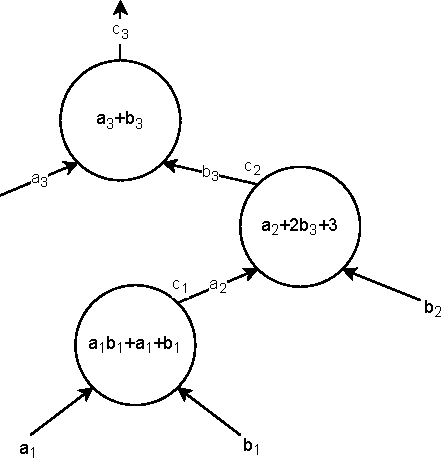
\includegraphics[width=0.4\textwidth]{../figures/plonk-circuit.drawio}
    \caption{Example of a \plonk-like circuit.}
    \label{figure:plonk-circuit-example}
\end{figure}

Observe all the values below depend only on the shape of the circuit itself, so if the circuit does not change, this polynomial should not be recomputed. Check that the \SA, \SB and \SC polynomials are constructed so that we can verify the copy-constraints $c_2 = b_3$ and $c_1 = a_2$ present in the circuit. Observe that equally painted cells have their values swapped, as explained before in the construction of the connection $S$ polynomials.  

\begin{figure}[H]
    \centering
    \begin{tabular}{|c|c|c|c|c|c|c|c|}
        \hline
        \QL	&\QR	&\QM	&\QO	&\QC	&\SA					&\SB						&\SC 							\\ \hline
        1			&1				&1				&-1				&0				&1								&$k_1$								&\cellcolor{pink} $g$				\\
        1			&2				&0				&-1				&3				&\cellcolor{pink}$k_2$			&$k_1 \cdot g$					&\cellcolor{cyan} $k_1 \cdot g^2$	\\
        1			&1				&0				&-1				&0				&$g^2$						&\cellcolor{cyan}$k_2 \cdot g$ &$k_2 \cdot g^2$					\\
        \hline
    \end{tabular}
    \label{table:plonk-circuit-example}
\end{figure}

Therefore, we can derive a PIL program that validates the previous circuit as shown below:
\begin{pil}
    include "config.pil";
    
    namespace Plonk(%N);
    pol constant QL, QR, QM, QO, QC;
    pol constant SA, SB, SC;
    pol constant L1;
    
    pol commit a, b, c;
    
    public pi = a(0);
    
    // Public values check 
    L1 * (a - :pi) = 0;
    
    // Plonk equation 
    pol ab = a*b;
    QL*a + QR*b + QM*ab + QO*c + QC = 0;
    
    // Copy-constraints check 
    {a, b, c} connect {SA, SB, SC};
\end{pil}




%%%%%%%%%%%%%%%%%%%%%%%%%%%%%%%%%%%%%%%%%%%%%%%%%%%%%%%%%%%%%%%%
\subsection{Filling Polynomials}

Until now we have only shown how to specify some kinds of constraints that several polynomials of a certain program described in PIL should satisfy to become \textit{correct}. All these constraints, together with the constant polynomials inherent to the computation itself, specify the transition function underlying the program definition. In other words, changing either any of the constraints or the description of the constant polynomials produces a change in the program we are working on. 

%TODO Check this paragraph
In this section, we are going to use Javascript and \pilcom to generate a specific execution trace for a given PIL. To do so, we are going to compute a valid execution trace for the example of Section \ref{sec:connecting-sm}. As a remark, we will also use the library \texttt{pil-stark} whose utility is to provide a framework to setup, generate and verify proofs, to use a \texttt{FGL} class which mimics a finite field and it is required by some functions that provide the \pilcom package. 

First of all, under the scope of an asynchronous function called \texttt{execute}, we parse the provided PIL (which is, in our case, \texttt{main.pil}) into a Javascript object using the \texttt{compile} function of \pilcom. In code we obtain:
\begin{js}
    const { FGL } = require("pil-stark");
    const { compile } = require("pilcom");
    const path = require("path");
    
    async function execute() {
        const pil = await compile(FGL, path.join(__dirname, "main.pil"));
    }
\end{js}

The \pilcom package also provides two functions that use the \texttt{pil} object to create two crucial objects from it for the construction of the execution trace: the constant polynomials object and the committed polynomials object (using \texttt{newConstPolsArray} and \texttt{newCommitPolsArray} functions, respectively).
\begin{js}
    const { newConstantPolsArray, newCommitPolsArray, compile } = require("pilcom");
    
    async function execute() {
        
        // ... Previous Code
        
        const constPols =  newConstantPolsArray(pil);
        const cmPols = newCommitPolsArray(pil);
    }
\end{js}

Both such objects contain useful information about the PIL itself, such as the provided length of the program $N$, the total number of constant polynomials and the total number of committed polynomials. However, accessing these objects will allow us to fill the entire execution trace for that PIL. We can access a specific position of the execution trace using the syntax:
\begin{js}
    pols.Namespace.Polynomial[i] 
\end{js}
being \texttt{pols} one of the previously introduced \texttt{constPols} and \texttt{cmPols} objects, \texttt{Namespace} being a specific namespace among the ones defined by the PIL files, \texttt{Polynomial} one of the polynomials defined under the scope of the previous namespace and $i$ an integer in the set $[0,N-1]$ representing the row of the current polynomial. Using this we can now start to fill our polynomials. 

In our example, we will use, as inputs for the trace, which are the ones introduced in the \texttt{Main.a} polynomial, an ascending chain of integers from $0$ to $15$ cyclically (because recall that we are only allowed to use $4$ bits integers). We propose here two functions that fill the constant and committed polynomials accordingly. 
\begin{figure}[H]
    \begin{js}
        async function buildConstantPolynomials(constPols, polDeg) {
            
            for (let i=0; i < polDeg; i++) {
                constPols.Global.BITS4[i] = BigInt(i & 0b1111);
                constPols.Global.L1[i] = i === 0 ? 1n : 0n;
                constPols.Negation.RESET[i] = (i % 4) == 3 ? 1n : 0n;
                constPols.Negation.FACTOR[i] = BigInt(1 << (i % 4));
                constPols.Negation.ISLAST[i] = i === polDeg-1 ? 1n : 0n;
            }
        }
    \end{js}
    \caption{Generation of the constant polynomials.}
\end{figure}

\begin{figure}[H]
    \begin{js}
        async function buildcommittedPolynomials(cmPols, polDeg) {
            
            cmPols.Negation.a[-1] = 0n;
            cmPols.Negation.neg_a[-1] = 1n;
            
            for (let i=0; i < polDeg; i++) {
                
                let fourBitsInt = i % 16;
                
                cmPols.Main.a[i] = BigInt(fourBitsInt);
                cmPols.Main.neg_a[i] = BigInt(fourBitsInt ^ 0b1111);
                cmPols.Main.op[i] = FGL.mul(cmPols.Main.a[i], cmPols.Main.neg_a[i]);
                
                cmPols.Multiplier.freeIn1[i] = cmPols.Main.a[i];
                cmPols.Multiplier.freeIn2[i] = cmPols.Main.neg_a[i];
                cmPols.Multiplier.out[i] = cmPols.Main.op[i];
                
                let associatedInt = Math.floor(i/4);
                let bit = (associatedInt >> (i%4) & 1) % 16;
                cmPols.Negation.bits[i] = BigInt(bit);
                cmPols.Negation.nbits[i] = BigInt(bit ^ 1);
                
                
                let factor = BigInt(1 << (i % 4));
                let reset = (i % 4) == 0 ? 1n : 0n;
                cmPols.Negation.a[i] = factor*cmPols.Negation.bits[i] 
                + (1n-reset)*cmPols.Negation.a[i-1];
                cmPols.Negation.neg_a[i] = factor*cmPols.Negation.nbits[i] 
                + (1n-reset)*cmPols.Negation.neg_a[i-1];
            }
        }
    \end{js}
    \caption{Generation of the committed polynomials.}
\end{figure}

Now that we have all the constant and committed polynomials filled in, we can check using a function called \texttt{verifyPil} that they indeed satisfy the constraints defined in the PIL file. We provide below the piece of code that construct the polynomials and check the constraints. If the verification procedure fails, we should not proceed to the proof generation because it will lead to false proof. 
\begin{js}
    const { newConstantPolsArray, newCommitPolsArray, compile, verifyPil } = require("pilcom");
    
    async function execute() {
        
        // ... Previous Code	
        
        const N = constPols.Global.BITS4.length;
        
        await buildConstantPolynomials(constPols, N);
        await buildcommittedPolynomials(cmPols, N);
        
        const res =  await verifyPil(FGL, pil, cmPols , constPols);
        if (res.length != 0) {
            console.log("The execution trace do not satisfy PIL restrictions. Aborting...");
            for (let i=0; i<res.length; i++) {
                console.log(res[i]);
                return;
            }
        }
    }
\end{js}







%TODO: Is this section necessary?
%%%%%%%%%%%%%%%%%%%%%%%%%%%%%%%%%%%%%%%%%%%%%%%%%%%%%%%%%%%%%%%%%
\subsection{Generating a Proof Using \texttt{pil-stark}}

Once the constant and the committed polynomials are filled, we can step to the proof generation stage. We can use the \texttt{pil-stark} Javascript package specially designed to work together with \pilcom to generate STARK proofs about PIL statements. We will use three functions \texttt{starkSetup}, \texttt{starkGen} and \texttt{starkVerify} from the package. The first one is aiming for setting up the STARK, which is independent of the values of committed polynomials. This includes the computation of the tree of the evaluations of the constant polynomials. For executing the setup generation we ought to have an object called \texttt{starkStruct} which is specifying several FRI-related parameters such as the size of the trace domain (which must coincide with $N$, defined in PIL), the size of the extended domain (which together with the previous parameter specifies the correspondent \textit{blowup factor}), the number of queries to be executed and the reduction factors for each of the FRI steps. We execute the setup using the code below:

\begin{js}
    const { FGL, starkSetup } = require("pil-stark");
    
    async function execute() {
        
        // ... Previous Code	
        
        const starkStruct = {
            "nBits": 10,
            "nBitsExt": 11,
            "nQueries": 128,
            "verificationHashType": "GL",
            "steps": [
            {"nBits": 11},
            {"nBits": 5},
            {"nBits": 3},
            {"nBits": 1}
            ]
        };
        
        const setup = await starkSetup(constPols, pil, starkStruct);
    }
\end{js}

Now that we have set up the STARK, we can generate the proof using the \texttt{starkGen} function. We can do this task using the code below. Observe that the \texttt{setup} object contains inside a \texttt{starkInfo} field which contains, aside from all the \texttt{starkStruct} parameters, lots of useful information about the shape of the PIL itself. 

\begin{js}
    const { FGL, starkSetup, starkGen } = require("pil-stark");
    
    async function execute() {
        
        // ... Previous Code	
        
        const resProof = await starkGen(cmPols, constPols, setup.constTree, setup.starkInfo);
    }
\end{js}

Now that a proof has been generated we can be involved in the verification procedure invoking the \texttt{starkVerify} function. This function needs, as arguments, some information provided by the outputs of both the \texttt{starkSetup} and \texttt{starkGen} functions. If the output of the \texttt{starkVerify} function is \texttt{true}, the proof is valid. Otherwise, the verifier should invalidate the proof sent by the prover. 

\begin{js}
    const { FGL, starkSetup, starkGen, starkVerify } = require("pil-stark");
    
    async function execute() {
        
        // ... Previous Code
        
        const resVerify = await starkVerify(
        resP.proof, resP.publics, setup.constRoot, setup.starkInfo
        );
        
        if (resVerify === true) {
            console.log("The proof is VALID!");
        } else {
            console.log("INVALID proof!");
        }
    }
\end{js}


%%%%%%%%%%%%%%%%%%%%%%%%%%%%%%%%%%%%%%%%%%%%%%%%%%%%%%%%%%%%%%% 
\section{zkASM instructions set} \label{sec:instructions}

\subsection{Memory Related Instructions}


We refer to the memory as a volatile read-write data storage that exists only during the execution of a zkASM program. The memory is divided into different contexts of \texttt{0x40000} words. Each word is 256 bits in length, so each context is 8 MB in size.

Each context is divided into the following three blocks:

\begin{itemize}
    
    \item \textbf{VARS:} With a relative offset of \texttt{0x00000} and a height of \texttt{0x10000} words (\texttt{2MB}), contains the local context variables pre-defined in the language. The list of all context variables can be found at \href[]{https://github.com/0xPolygonHermez/zkevm-rom/blob/main/main/vars.zkasm}{\texttt{vars.zkasm}}.
    
    \item \textbf{STACK:} With a relative offset of \texttt{0x10000} and a height of \texttt{0x10000}  words  \texttt{(2MB)}, contains the stack of the the EVM. \textbf{STACK} is defined once per context.
    
    \item \textbf{MEMORY:} With a relative offset of \texttt{0x20000} and a height of \texttt{0x20000} words \texttt{(4MB)}, contains the free memory that can be freely used. \textbf{MEMORY}, like \textbf{STACK}, is also defined once per context. 
\end{itemize}

Therefore, for a given slot in memory, its pointer is computed as:
\[
\texttt{memoryAddress} = \texttt{0x40000} \cdot \texttt{CTX} + \texttt{isStack} \cdot (\texttt{0x10000} + \texttt{SP}) + \texttt{isMem} \cdot (\texttt{0x20000} + \texttt{offset})
\]
where:

\begin{itemize}
    
    \item \texttt{CTX}: This integer variable refers to the memory context being accessed in the EVM's memory. 
    
    \item \texttt{isStack}:  this boolean value indicates whether the memory operation being performed is related to the EVM's stack. The EVM uses a stack-based architecture, meaning that operations are performed by pushing and popping values on and off the stack.
    
    \item \texttt{SP}: This variable refers to the current position of the stack pointer in the EVM's stack. The stack pointer is used to keep track of the current top of the stack. More information on \texttt{SP} will be added below.
    
    \item \texttt{isMem}: This boolean value indicates whether the memory operation being performed is related to the EVM's memory. Observe that \texttt{isStack} and \texttt{isMem} can not be $1$ at the same time. 
    
    \item \texttt{offset}:  This variable likely refers to the offset or location within the current memory context being accessed.
    
\end{itemize}

Observe that, following the above description of the memory, the former set of variables completely determine a memory slot. Figure ?? shows the structure of the memory during a zkASM execution.

\begin{figure}[H]
    \centering
    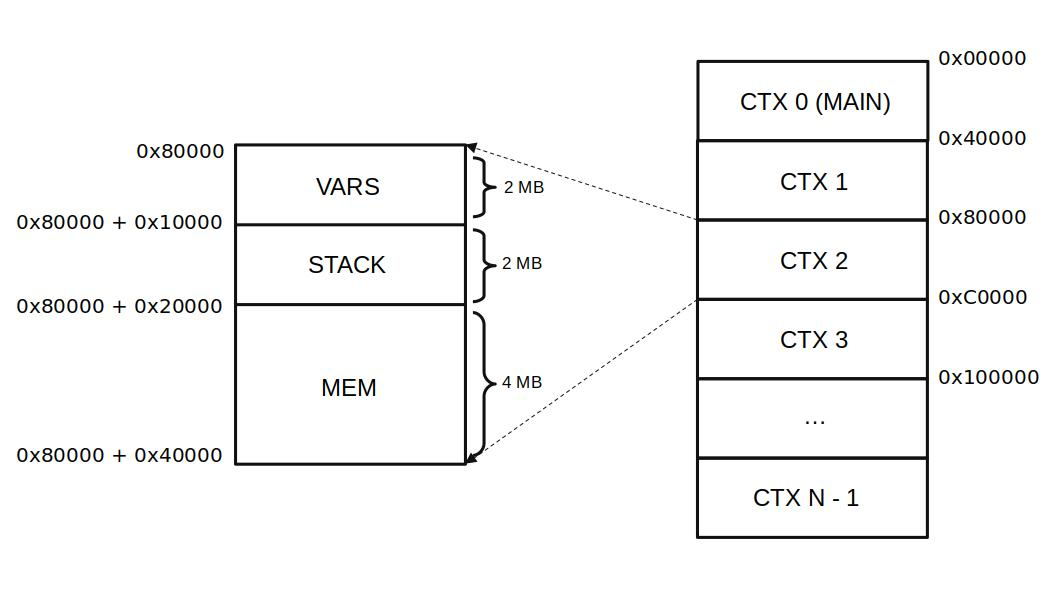
\includegraphics[width=0.6\columnwidth]{\assemblydir/figures/memory-regions}
    \caption{Schema of contexts and memory regions of the zkEVM.}
    \label{fig:memory-regions}
\end{figure}

In order to allow runtime interaction with memory, zkASM has a couple of instructions to read and write values to it.



Let us first define how can be access to a specific address of the memory. Memory acess will be parametrized by $2$ integer parameters: the address \addr and the relative address \relAddr. 

\begin{itemize}

\item \addr: Address would be able to define a memory access up to memory region level. That is, \addr will contain information of which context access the memory and if the access is directed to the system variables \textbf{VARS}, the \textbf{STACK} or the \textbf{MEMORY}.

\item \relAddr: However, \addr is not enough. Hence, \relAddr will point to a specific memory slot inside a concrete memory region of a context. We should take into account that \relAddr can never be negative. Moreover, \relAddr is also bounded from above: if we are accessing to the \textbf{MEMORY}, \relAddr should be strictly less than \texttt{0x40000} (because memory measures $\texttt{4MB}$) and if we are accessing to the \textbf{STACK} or to the system variables \textbf{VARS}, \relAddr should be strictly less than \texttt{0x10000} (because both memory regions measure $\texttt{2MB}$). Then, the wanted memory slot will be equal to $\addr + \relAddr$.

\end{itemize}

Let us know how to specify \addr and \relAddr in zkASM language. We can specify \addr with $3$ keywords: \texttt{SYS} (which corresponds to \textbf{VARS} memory region), \texttt{STACK} (which corresponds to \textbf{STACK} memory region) and \texttt{MEM} (which corresponds to \textbf{MEMORY} memory region). Invoking \texttt{STACK} will increase \addr by $\texttt{0x10000}$ and similarly, invoking \texttt{MEM} will increase \addr by \texttt{0x20000}. However, since \textbf{VARS} is the first memory region, it will not produce an increase in \addr. Moreover, \addr will also increase depending on the current context. More specifically, a total amount of \texttt{0x40000} will be increased per context, following our memory description above. 

To specify \relAddr we can use $2$ registers: \E and \RR. If \E is chosen, \relAddr will increase a total amount of $\E_0$ units. Similarly, if \RR is chosen, \relAddr will increase by \RR. Moreover, we can add a numeric offset to increase a fixed amount of units \addr + \relAddr. 

The syntax will be, in each case:

\begin{zkasm}
addr:relAddr 
; or
addr:relAddr+offset
; or 
addr:relAddr-offset
\end{zkasm}

Below, we specify concrete examples on how to specify addresses:

\begin{zkasm}
SYS:E
SYS:E+1
STACK:RR
MEM:E 
MEM:E-2
MEM:RR+1
\end{zkasm}

To end up, we can also access to addresses by means of global and local variables, defined elsewhere in the assembly code. This variables will have a unique identifier that we will use in order to access to it.


\subsubsection{\MLOAD}


\MLOAD is the zkASM instruction used to read a value from a specific address in memory. It takes the pointer address of the memory slot to be read as a parameter. We can store the value that is read in a register of our choosing by using the free input (\texttt{\$}) assignment. 

Suppose that we want to read the memory value stored in the address \texttt{someAddr} in a certain context. The address \texttt{someAddr} is defined by the global variable:
\begin{zkasm}
VAR GLOBAL someAddr
\end{zkasm}

The following zkASM code stores the corresponding value into the register \A:
\begin{zkasm}
$ => A          :MLOAD(someAddr)
\end{zkasm}





\subsubsection{\MSTORE}


\MSTORE is the zkASM instruction used to write a value to a specific address in memory. It takes the pointer address of the memory slot to be read as a parameter, the register that contains the value to be writed must be also specified.

The following example shows how to store in the memory the value of the current context. Note that as the \MSTORE parameter, it is specified the variable that contains the pointer to where current context is stored in the memory. The value stored will be taken from \texttt{CTX} register:
\begin{zkasm}
CTX       :MSTORE(currentCTX)      
\end{zkasm}



\subsubsection{Dealing with the STACK}

A stack machine is a machine in which temporary values for computations are moved to and from a push down stack. Operations over the stack are the typical: \texttt{PUSH}, \texttt{POP}, \texttt{DUP}, \texttt{SWAP}, etc. Since the EVM is a stack-based virtual machine, we reserve an address space to create a stack within the memory of the zkEVM. The classical pointer called \texttt{STACK POINTER} (\texttt{SP}) contains the address of the \textbf{next free position on the} \texttt{STACK}. A \texttt{POP} from the \texttt{STACK} can be implemented as:

\begin{zkasm}
SP -1 => SP
$ => A		:MLOAD(SP)
\end{zkasm}

where we decrement \texttt{SP} to reposition it on the last element of the stack and
then we load this element into registry \A. Similarly, a \texttt{PUSH} into the \texttt{STACK} can be implemented as:

\begin{zkasm}
0		:MSTORE (SP++)
\end{zkasm}

which saves a \texttt{0} at the top of the stack and increments \texttt{SP}. An important note about both the stack and the memory is that the stack pointer and the memory are per context.




\subsubsection{\MEMALIGNRD}

Although the memory word in zkASM is 256 bits long, in roder to mimic the regular Ethereum Virtual Machine (EVM) memory behavior, zkASM has a specific instructions for accessing memory at the byte level. The instruction \MEMALIGNRD enables reading 32 bytes starting from an offset of any byte in memory. In this way, two memory registers are read and a the following transformation is applied to virtually obtain a new 32-byte word as a result of the reading.
\begin{align*}
    \texttt{val} &= \Bigr[ \texttt{m}_0 \ll 8 \cdot \texttt{offset} \Bigr] \mathbin\Vert \Bigr[ \texttt{m}_1 \gg 256- 8 \cdot \texttt{offset} \Bigr] 
\end{align*}

Here, the symbol $\mathbin\Vert$ denotes string concatenation. The registers must be set as follows before call the \MEMALIGNRD instruction. We can store the value that is read in a register of our choosing by using the free input (\texttt{\$}) assignment.


\begin{figure}[h!]
    \renewcommand{\figurename}{Table}
    \[
    \begin{array}{|c|c|}
        \hline
        \mathbf{Register} &\mathtt{MEM\_ALIGN\_RD} \ \mathbf{parameters} \\ \hline
        \A & \texttt{Memory Slot of } \mathtt{m_0} \\
        \B & \texttt{Memory Slot of } \mathtt{m_1} \\
        \C & \texttt{offset} \\
        \hline
    \end{array}
    \]
    \caption{\MEMALIGNRD instruction parameters.}
    \label{tab:memory-first-example}
\end{figure}

The following example shows how to read 32 bytes that are stored occupying part of two consecutive zkASM memory words. The read value will be stored in register \A:

\begin{zkasm}
$ => A          :MLOAD(someAddr)
$ => B          :MLOAD(someAddr+1)
16 => C

$ => A          :MEM_ALIGN_RD
\end{zkasm}

Figure ?? shows how the 32-bytes value will be read for the \MEMALIGNRD given example.

\begin{figure}[H]
    \centering
    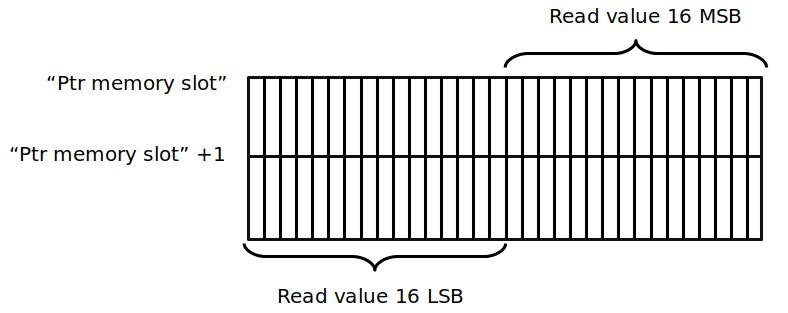
\includegraphics[width=0.8\columnwidth]{\assemblydir/figures/mem-align-wr}
    \caption{Example of how values are read from the memmory using \MEMALIGNRD with an offset of 16.}
    \label{fig:memory-regions}
\end{figure}

\subsubsection{\MEMALIGNWR}
\MEMALIGNWR is equivalent to \MEMALIGNRD but for writing a 32-byte value. In this case, we have to specify two memory slots that will be written after applying the following transformation to the value to be stored. The registers that contains the value to be stored must also be specified.
\begin{align*}
    \texttt{w}_0 &= \Bigr[ \texttt{m}_0 \ \texttt{\&} \ \left(2^{256} - 2^{256-8 \cdot \texttt{offset}} \right) \Bigr] \mathbin\Vert \Bigr[  \texttt{val} \ll 8 \cdot \texttt{offset} \Bigr]  \\
    \texttt{w}_1 &= \Bigr[ \texttt{m}_1 \ \texttt{\&} \ \left( \left( 2^{256} - 1\right)  \gg 8 \cdot \texttt{offset}\right) \Bigr] \mathbin\Vert \Bigr[ \texttt{val} \ll 8 \cdot \texttt{offset} \Bigr] 
\end{align*}

\begin{figure}[h!]
    \renewcommand{\figurename}{Table}
    \[
    \begin{array}{|c|c|}
        \hline
        \mathbf{Register} &\mathtt{MEM\_ALIGN\_WR} \ \mathbf{parameters} \\ \hline
        \A & \texttt{Memory Slot of } \mathtt{m_0}  \\
        \B & \texttt{Memory Slot of } \mathtt{m_1}  \\
        \C & \mathtt{offset} \\
        \D & \mathtt{w_0} \\
        \E & \mathtt{w_1} \\
        \op& \texttt{Value to be written} \\
        \hline
    \end{array}
    \]
    \caption{\MEMALIGNWR instruction parameters.}
    \label{tab:memory-first-example}
\end{figure}

The following example shows how to write 32 bytes that are stored occupying part of two consecutive zkASM memory words. The value to be stored will be taken from free input register:

\begin{zkasm}
$ => A          :MLOAD(MEM:E)
$ => B          :MLOAD(MEM:E+1)

${memAlignWR_W0(A,mem.bytesToStore,C)} => D                    ; no trust calculate W0
${memAlignWR_W1(B,mem.bytesToStore,C)} => E                    ; no trust calculate W1
$               :MEM_ALIGN_WR,MLOAD(bytesToStore)
\end{zkasm}

\subsubsection{\MEMALIGNWRE}

\MEMALIGNWRE allows writing only 8 bits of a specific memory slot. In this case, we have to specify the memory slot to be written, the register that contains the byte to be stored, and the offset value that situates the byte in a specific position of the 32-byte word. The value will be written after applying the following transformation:
\begin{align*}
    \texttt{w}_0 &= \Bigr[ \texttt{m}_0 \ \texttt{\&} \ \left( \texttt{maskByte} \gg 8 \cdot \texttt{offset} \right) \Bigr]  \mathbin\Vert \Bigr[ \left( \texttt{bits} \ \texttt{\&} \ \texttt{0xFF} \right)  \ll 8 \cdot \left( 31-\texttt{offset}\right) \Bigr] 
\end{align*}
where $\texttt{maskByte}$ equals $2^{256} - 1$. 

\begin{figure}[h!]
    \renewcommand{\figurename}{Table}
    \[
    \begin{array}{|c|c|}
        \hline
        \mathbf{Register} &\mathtt{MEM\_ALIGN\_WR8} \ \textbf{parameters} \\ \hline
        \A & \texttt{Memory Slot of } \mathtt{m_0} \\
        \C & \mathtt{offset} \\
        \D & \mathtt{w_0} \\
        \op& \texttt{Value to be written} \\
        \hline
    \end{array}
    \]
    \caption{\MEMALIGNWRE instruction parameters.}
    \label{tab:memory-first-example}
\end{figure}

The following example shows how to write $1$ bytes stored in the byte $4$ of a specific storage slot. The value to be stored will be taken from \B register:

\begin{zkasm}
4 => C
$ => A          :MLOAD(someAddr)
${memAlignWR8_W0(A,B,C)} => D  ; no trust calculate W0
B               :MEM_ALIGN_WR8 ; only use LSB of B, rest of bytes could be non zero
\end{zkasm}

\subsection{Storage Related Instructions}

Polygon zkEVM, like Ethereum L1, has a storage component for storing persistent on-chain data, which includes the balances of all accounts, their nonces, and the state of all deployed smart contracts along with their codes. The data that forms the state is represented as cryptographic trie, but while Ethereum L1 uses a modified Patricia tree with Keccak256 as the hash operation, Polygon zkEVM uses a binary sparse Merkle tree with Poseidon as the hash operation (refer to the technical documents regarding the zkEVM bridge annex A to learn more about sparse Merkle trees).

Poseidon is a hash function that's specifically designed for use in zero-knowledge applications, as it's meant to operate with values of a prime field and it has been proven to be much more performant than Keccak256 in zero-knowledge constructions like those used in Polygon zkEVM. Moreover Poseidon hash has an input named capacity, which can be used as an extra input value.

Barely, the Polygon zkEVM state tree is a key-value structure in which the integrity can be ensured by a 256-bit value known as the state root. Each entry in the tree is a leaf and directly stores a 256-bit value. Additionally, the index position of that leaf in the tree corresponds to the 256-bits of the key. As can be seen in Figure X, since the keys are 256-bits in length, the tree has 32 levels and a total capacity of $2^{256}$ leaves.


\begin{figure}[H]
    \centering
    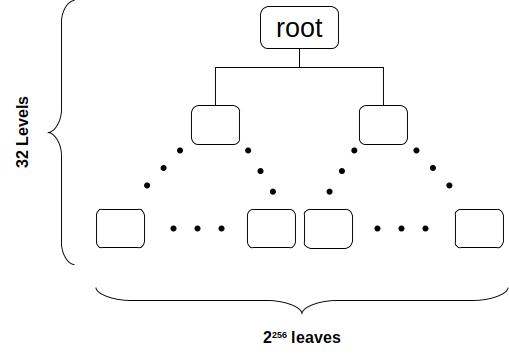
\includegraphics[width=0.6\columnwidth]{\assemblydir/figures/state-trie}
    \caption{Polygon zkEVM state trie.}
    \label{fig:hashk-add-bytes}
\end{figure}

Since five different types of values can be stored, a distinction must be made among the five types of leaves. Table X shows the relation between leaf type and the corresponding data types that they contain.

\begin{figure}[h!]
    \renewcommand{\figurename}{Table}
    \[
    \begin{array}{|c|c|}
        \hline
        \mathbf{Leaf~type} &\mathbf{Data~type} \\ \hline
        \mathtt{0} & \mathtt{Account~balance} \\
        \mathtt{1} & \mathtt{Account~nonce} \\
        \mathtt{2} & \mathtt{Contract~code~hash} \\
        \mathtt{3} & \mathtt{Contract~storage~slot~value} \\
        \mathtt{4} & \mathtt{Contract~code~length} \\
        \hline
    \end{array}
    \]
    \caption{Polygon zkEVM state tree leaf types.}
    \label{tab:memory-first-example}
\end{figure}


For each leaf entered in the tree its key is computed as follows:

$$\texttt{key} = \texttt{Poseidon}(\texttt{key\_seed})$$

where \texttt{key\_seed} is a $32$-bytes integer constructed as follows:
\[
\texttt{key\_seed} = (\texttt{account\_address} \mid\mid \texttt{0x00000000} \mid\mid \texttt{leaf\_type} \mid\mid \texttt{0x00000000})
\]
being $\texttt{account\_address} \in \{0, 1, \dots, 2^{160} - 1\}$ is a $20$-bytes integer and $\texttt{leaf\_type} \in \{0, 1, \dots, 2^{32} - 1\}$ a $4$-bytes integer.

The capacity of the Poseidon's instance used when computing keys is always zero except in the case where the leaf corresponds to a contract storage slot value (leaf type 3), in which case the capacity is directly set to the storage slot pointer. It's important to note that because the contract storage slot pointer is not encoded in the 32-byte input, if we do not use the capacity, all storage slots for the same contract would lead to the same state tree leaf.

Te value sored in the leaf has the following structure:
\[
(v_0, \dots, v_7)
\]
codifying a $256$-bits unsigned integer, where $v_i \in \FF_p$ are bounded to $32$-bits each. 

In order to allow runtime interaction with the Polygon zkEVM state tree zkASM has a couple of instructions to read and write values on it.

\subsubsection{\texttt{SLOAD}}

\texttt{SLOAD} is the zkASM instruction used to read a value from a leaf in the state tree. It takes Poseidon's ``Input" and ``Capacity" parameters, along with the leaf type, to compute the key of the leaf to be read. The registers must be set as follows before call the \texttt{SLOAD} instruction.

\begin{figure}[h!]
    \renewcommand{\figurename}{Table}
    \[
    \begin{array}{|c|c|}
        \hline
        \mathbf{Register} &\texttt{SLOAD } \textbf{parameters} \\ \hline
        \A & \mathtt{Account~address} \\
        \B & \mathtt{Leaf~type} \\
        \C & \mathtt{Contract~storage~slot~pointer~(capacity)} \\
        \hline
    \end{array}
    \]
    \caption{\texttt{SLOAD} instruction parameters.}
    \label{tab:memory-first-example}
\end{figure}

We can store the value that is read in a register of our choosing by using the free input (\texttt{\$}) assignment.

The following example shows how to read the balance of a specific account, the value that is read will be stored in the \E register:

\begin{zkasm}
someAccountAddr => A          
0 => B      
0 => C          
$ => E          :SLOAD
\end{zkasm}

The following example shows how to read a storage slot of a specific contract, the value that is read will be stored in the \E register:

\begin{zkasm}
someAccountAddr => A          
3 => B      
storageSlotPtr => C 
$ => E          :SLOAD
\end{zkasm}

\subsubsection{\texttt{SSTORE}}

\texttt{SSTORE} is the zkASM instruction used to store a value to a leaf in the state tree. It takes Poseidon's ``Input" and ``Capacity" parameters, along with the leaf type, to compute the key of the leaf to be writen, in addition takes the value to be written. The registers must be set as follows before call the \texttt{SSTORE} instruction.

\begin{figure}[h!]
    \renewcommand{\figurename}{Table}
    \[
    \begin{array}{|c|c|}
        \hline
        \mathbf{Register} &\texttt{SSTORE } \textbf{parameters} \\ \hline
        \A & \mathtt{Account~address} \\
        \B & \mathtt{Leaf~type} \\
        \C & \mathtt{Contract~storage~slot~pointer~(capacity)} \\
        \D & \mathtt{Value~to~write} \\
        \hline
    \end{array}
    \]
    \caption{\texttt{SSTORE} instruction parameters.}
    \label{tab:memory-first-example}
\end{figure}

The following example shows how to write a storage slot of a specific contract:

\begin{zkasm}
someAccountAddr => A          
3 => B      
storageSlotPtr => C          
value => D         
A               :SSTORE
\end{zkasm}




%%%%%%%%%%%%%%%%%%%%%%%%%%%%%%%%%%%%%%%%%%%%%%%%%%%%%%%%%%%%%%%

\subsection{Binary-Related Instructions}

The arithmetic operators are used to perform arithmetic mathematical operations on numeric data stored in registers.

\subsubsection{\ADD}

\ADD is used to sum the content of the registers \A and \B, the result will be treated as a free input. The following example shows how to use \ADD instruction.

\begin{zkasm}
val1 => A          
val2 => B          

$ => C             :ADD ; [ val1 + val2 => C]
\end{zkasm}

\subsubsection{\SUB}

\SUB is used to subtract de content fo register \B to \A, the result will be treated as a free input. The following example shows how to use \SUB instruction.

\begin{zkasm}
val1 => A          
val2 => B          

$ => C             :SUB ; [ val1 - val2 => C]
\end{zkasm}



\subsubsection{\LT}

\LT instruction is used to compare the values of the registers \A and \B as \textbf{unsigned integers}. The output of the operation will be $1$ if \A is actually lower than \B (that is, $\A < \B$) and $0$ otherwise (that is, $\A \geq \B$). The output of the instruction will be treated as a free input. The next lines of code show an example on how to use \LT instruction:

\begin{zkasm}
valA => A
valB => B

$ => C			:LT ; [1 if A < B, 0 if A <= B]
\end{zkasm}





\subsubsection{\SLT}

\SLT instruction is used to compare the values of the registers \A and \B as \textbf{signed integers}, explained in Section \ref{sec:binary-sm}. The output of the operation will be $1$ if \A is actually lower than \B (that is, $\A < \B$) and $0$ otherwise (that is, $\A \geq \B$). The output of the instruction will be treated as a free input. The next lines of code show an example on how to use \SLT instruction:

\begin{zkasm}
valA => A
valB => B

$ => C			:SLT ; [1 if A < B, 0 if A <= B]
\end{zkasm}


\subsubsection{\EQ}

\EQ instruction is used to compare the equality relationship between the values of the registers \A and \B. The output of the operation will be $1$ if \A is equal to \B (that is, $\A = \B$) and $0$ otherwise (that is, $\A \neq \B$). The output of the instruction will be treated as a free input. The next lines of code show an example on how to use \EQ instruction:

\begin{zkasm}
valA => A
valB => B

$ => C			:EQ ; [1 if A = B, 0 if A != B]
\end{zkasm}


\subsubsection{\AND}


\AND instruction is used to perform the bit-wise \AND operation between registers \A and \B, as explained in Section \ref{sec:binary-sm}. The output of the instruction will be treated as a free input. The next lines of code show an example on how to use \AND instruction:

\begin{zkasm}
valA => A
valB => B

$ => C			:AND
\end{zkasm}

For sake of completeness, let us propose a more concrete example, where we assign the value $\texttt{0xDBn}$ to \A and the value $\texttt{0x86n}$ to \B. The result of the bit-wise \AND operation is going to be \texttt{0x82n} because
\[
\A = \texttt{0b11011011}, \quad \B = \texttt{0b10000110} \Longrightarrow \C = \texttt{0b10000010}.
\]

\begin{zkasm}
0xDBn => A
0x86n => B

$ => C			:AND ; C = 0x82n
\end{zkasm}

\subsubsection{\OR}

\OR instruction is used to perform the bit-wise \OR operation between registers \A and \B, as explained in Section \ref{sec:binary-sm}. The output of the instruction will be treated as a free input. The next lines of code show an example on how to use \OR instruction:

\begin{zkasm}
valA => A
valB => B

$ => C			:OR
\end{zkasm}

For sake of completeness, let us propose a more concrete example, where we assign the value $\texttt{0xDBn}$ to \A and the value $\texttt{0x86n}$ to \B. The result of the bit-wise \OR operation is going to be \texttt{0xDFn} because
\[
\A = \texttt{0b11011011}, \quad \B = \texttt{0b10000110} \Longrightarrow \C = \texttt{0b11011111}.
\]

\begin{zkasm}
0xDBn => A
0x86n => B

$ => C			:OR ; C = 0xDFn
\end{zkasm}



\subsubsection{\XOR}

\XOR instruction is used to perform the bit-wise \XOR operation between registers \A and \B, as explained in Section \ref{sec:binary-sm}. The output of the instruction will be treated as a free input. The next lines of code show an example on how to use \XOR instruction:

\begin{zkasm}
valA => A
valB => B

$ => C			:XOR
\end{zkasm}

For sake of completeness, let us propose a more concrete example, where we assign the value $\texttt{0xDBn}$ to \A and the value $\texttt{0x86n}$ to \B. The result of the bit-wise \XOR operation is going to be \texttt{0x5Dn} because
\[
\A = \texttt{0b11011011}, \quad \B = \texttt{0b10000110} \Longrightarrow \C = \texttt{0b01011101}.
\]

\begin{zkasm}
0xDBn => A
0x86n => B

$ => C			:XOR ; C = 0x5Dn
\end{zkasm}





%%%%%%%%%%%%%%%%%%%%%%%%%%%%%%%%%%%%%%%%%%%%%%%%%%%%%%%%%%%%%%%
\subsection{Arithmetic-Related Instructions}

\subsubsection{\ARITH}

The \ARITH instruction allows to check field operations. More specifically, it checks a combination of an addition and a product, as explained in Section \ref{sec:arith-sm}. Before calling the \ARITH instruction, registers \A, \B, and \C must be set. The equation that follows will be evaluated using the values of these $3$ registers. It is necessary to specify where the result of the evaluation will be stored. If the evaluation results in an overflow of the output register, the overflow value will be stored in register \D. More specifically, the equation that checks the \ARITH instruction is the following one:

\[
\D \cdot 2^{256} + \op = \A \cdot \B + \C
\]

The following example shows how to use \ARITH instruction. The result of the evaluation will be stored in register \A, and if there is an overflow, it will be stored in register \D:
\begin{zkasm}
valA => A          
valB => B          
valC => C
A            :ARITH ; [ valA * valB + valC => [D,A]]
\end{zkasm}





\subsubsection{\ARITHADDDIFF}

The \ARITHADDDIFF instruction allows to perform additions $P + Q$ over the elliptic curve defined in Section \ref{sec:arith-sm}. This instruction can not perform doublings, since the input points to be added are supposed to be different. This is not explicitly check, but since the doubling formula differs a lot from the distinct point addition formula, the result will be wrong if $P = Q$. The input parameters of the instruction are specified in the table below:

\begin{figure}[h!]
    \renewcommand{\figurename}{Table}
    \[
    \begin{array}{|c|c|}
        \hline
        \mathbf{Register} &\texttt{ARITH\_ECADD\_DIFFERENT } \textbf{parameters} \\ \hline
        \A & x_1, \mathtt{~x~coordinate~of~}P \\
        \B & y_1, \mathtt{~y~coordinate~of~}P \\
        \C & x_2, \mathtt{~x~coordinate~of~}Q \\
        \D & y_2, \mathtt{~y~coordinate~of~}Q \\
        \E & x_3, \mathtt{~x~coordinate~of~}P+Q \\
        \op & y_3, \mathtt{~y~coordinate~of~}P+Q \\
        \hline
    \end{array}
    \]
    \caption{\ARITHADDDIFF instruction parameters.}
    \label{tab:memory-first-example}
\end{figure}

An example on how to use the \ARITHADDDIFF instruction can be seen in the code blow. Observe that we make use of the executor implemented functions \texttt{xAddPointEc(A,B,C,D)} and \texttt{yAddPointEc(A,B,C,D)} which compute the $x$ and the $y$ coordinate of $P + Q$ being $P = (A, B)$ and $Q = (C, D)$ whenever $P \neq Q$. After this is computed, the $x$ coordinate of $P + Q$ is is stored into the memory slot given by the address \texttt{addX} and, similarly, the $y$ coordinate of $P + Q$ is pushed into the memory slot given by the address \texttt{addY}. If we have used incorrect values for the coordinates of $P + Q$, an executor error will pop. This will also be captured when the proof of the batch is generated, since the instruction invocation fills the polynomials of the Arithmetic State Machine correctly. 

\begin{zkasm}
$ => A  						:MLOAD(Px)
$ => B  						:MLOAD(Py)
$ => C  						:MLOAD(Qx)
$ => D  						:MLOAD(Qy)
${xAddPointEc(A,B,C,D)} => E  	:MSTORE(addX)
${yAddPointEc(A,B,C,D)} 		:ARITH_ECADD_DIFFERENT, MSTORE(addY)
\end{zkasm}


\subsubsection{\ARITHADDSAME}

The \ARITHADDSAME instruction allows to perform point doublings $2P$ over the elliptic curve defined in Section \ref{sec:arith-sm}. The input parameters of the instruction are specified in the table below:

\begin{figure}[h!]
    \renewcommand{\figurename}{Table}
    \[
    \begin{array}{|c|c|}
        \hline
        \mathbf{Register} &\texttt{ARITH\_ECADD\_DIFFERENT } \textbf{parameters} \\ \hline
        \A & x_1, \mathtt{~x~coordinate~of~}P \\
        \B & y_1, \mathtt{~y~coordinate~of~}P \\
        \E & x_3, \mathtt{~x~coordinate~of~}2P \\
        \op & y_3, \mathtt{~y~coordinate~of~}2P \\
        \hline
    \end{array}
    \]
    \caption{\ARITHADDDIFF instruction parameters.}
    \label{tab:memory-first-example}
\end{figure}

An example on how to use the \ARITHADDSAME instruction can be seen in the code blow. Observe that we make use of the executor implemented functions \texttt{xDblPointEc(A,B)} and \texttt{yDblPointEc(A,B)} which compute the $x$ and the $y$ coordinate of $2P$ being $P = (A, B)$. After this is computed, the $x$ coordinate of $2P$ is is stored into the memory slot given by the address \texttt{doublePx} and, similarly, the $y$ coordinate of $2P$ is pushed into the memory slot given by the address \texttt{doublePy}. If we have used incorrect values for the coordinates of $2P$, an executor error will pop. This will also be captured when the proof of the batch is generated, since the instruction invocation fills the polynomials of the Arithmetic State Machine correctly. 

\begin{zkasm}
$ => A  					:MLOAD(Px)
$ => B  					:MLOAD(Py)

${xDblPointEc(A,B)} => E  	:MSTORE(doublePx)
${yDblPointEc(A,B)} 		:ARITH_ECADD_SAME, MSTORE(doublePy)
\end{zkasm}









%%%%%%%%%%%%%%%%%%%%%%%%%%%%%%%%%%%%%%%%%%%%%%%%%%%%%%%%%%%%%%%
\subsection{Execution Control Flow Related Instructions}

In order to allow to conditional branch execution of the zkASM programs, 4 different instruction has been included in zkASM instructios set.

\subsubsection{\JMP} % Jump
\JMP is an unconditional jump instruction that always causes a jump in the program's execution flow, regardless of any conditions. It takes an address of the ROM as a parameter to continue the execution flow. To avoid using numeric pointers for jumps, zkASM allows jump destinations to be aliased with custom names. The compiler resolves these aliases and substitutes them with pointers later on.

The following code shows the general usage of \JMP instruction:

\begin{zkasm}
    
; ...
; Executed Code
; ...

        :JMP(destinationLabel)

; ... 
; Non Executed Code
; ... 

destinationLabel:

; ...
; Executed Code
; ...
    
\end{zkasm}

Moreover, we can also parametrize the destination of a jump-like instruction using either the first limb of the register $\E_0$ or the register \RR, using the syntax below:

\begin{zkasm}
        :JMP(RR)
        :JMP(E)
\end{zkasm}

For example, the code below will produce a jump of $5$ units in the execution flow:

\begin{zkasm}
5 => E
            :JMP(E)          
\end{zkasm}

The former syntax will be also available for all the other kind of jumps specified in below sections, including the ones having an else clause.

\subsubsection{\JMPN} % Jump if Negative

\JMPN is a conditional jump instruction that causes a jump in the program's execution flow if a specified register contains a negative number. It takes the address of the ROM as a parameter to continue the execution flow. The register that contains the value to be evaluated must also be specified.

In the following example, the execution flow will be redirected to \texttt{stackUnderflow} in the case that the evaluation of $\SP - 2$ leads to a negative number.

\begin{zkasm}
; check stack underflow
SP - 2          :JMPN(stackUnderflow)
\end{zkasm}

Conditional jumps can also receive an else-clause label. The synatx is very similar:

\begin{zkasm}
A					:JMPN(ifClauseLabel, elseClauseLabel)


ifClauseLabel:
        ; do something
        
        
elseClauseLabel:
        ; do something different
\end{zkasm}

If the value stored in the \A register is negative, then the execution of the program will continue under the \texttt{ifClauseLabel} label. However, if the value of \A is bigger or equal than $0$, then the execution will continue from the label \texttt{elseClauseLabel}. 




\subsubsection{\JMPC} % Conditional jump, if a condition is fullfiled

\JMPC is a conditional jump instruction that causes a jump in the program's execution flow if a specified condition is evaluated  as true. It is used along with the following comparative instructions.
\begin{itemize}
    \item \EQ: Evaluates if register \A value is equal to register \B value.
    \item \LT: Evaluates if register \A value is less than register \B value.
    \item \SLT: Evaluates if register \A value is less than register \B value also comparing negative values.
\end{itemize}

In the following example, the execution flow will be redirected to \texttt{absIsNeg} in the case that the value contained in register \A (namely \val) is a negative number.

\begin{zkasm}
val => A
0 => B
$          :SLT, JMPC(absIsNeg)
\end{zkasm}





\subsubsection{\JMPZ} % Jump if Zero

\JMPZ is a conditional jump instruction that causes a jump in the program's exectuion flow if a specified register contains a 0. In the following example, the execution flow will be redirected to \texttt{readCode} in the case that the value contained in register \A (namely \val) is $0$.

\begin{zkasm}
val => A
A                   :JMPZ(readCode)
\end{zkasm}






\subsubsection{\JMPNC and \JMPNZ}

In addition to all the previously defined execution jumps, there are two more jumps: \JMPNC and \JMPNZ. This kind of jumps works the other way around \JMPC and \JMPZ does. More concretely, in the code below, the execution will jump to the label \texttt{someLabel} if and only if the value stored in the register \A \textbf{is not} zero. Otherwise, if the condition is satisfied, the execution will proceed normally.
\begin{zkasm}

A			:JMPNZ(someLabel)


someLabel:
    ; do something
\end{zkasm}

Hence, the first argument appearing in the instruction denotes now the else-clause. In fact, we can also adopt an if-else structure in this kind of negated instructions:

\begin{zkasm}

A			:JMPNZ(elseLabel, ifLabel)

elseLabel:
    ; do something
    
ifLabel:
    ; do something
\end{zkasm}

In the above piece of code, if the value of \A is not zero, then the execution will jump to the label \texttt{elseLabel} and, otherwise, it will jump to \texttt{ifLabel}. 



\subsubsection{\ASSERT}
\ASSERT is used to ensure that a given register has the same value as register \A. A failing assertion, meaning that the values are unequal, will stop execution and throw error during runtime. Additionally, an execution that contains a failing assertion cannot generate a valid CI proof.

The following code will compare $\val_1$ with $\val_2$, and if they are not equal the execution will be immediately stopped:

\begin{zkasm}
val1 => A
val2 => B
B    		:ASSERT
\end{zkasm}


\subsubsection{Subroutines (\CALL and \RETURN)}


Subroutines allow breaking down the code into smaller sections that can be called by using only a \CALL instruction. A subroutine is designed to be reusable and can be called by other parts of the program. The code of a subroutine always ends with a \RETURN instruction. When a subroutine is called, control is transferred from the main program to the subroutine. The subroutine then executes its code and, when it's finished, control is returned to the point in the main program immediately following the point where the subroutine was called.

An example of subroutine can be the \texttt{ecrecover\_tx} subrutine used in the zkEVM ROM, it is used to recover the signer of a specific ethereum transaction. zkASM code of \texttt{ecrecover\_tx } subrutine can be found \href[]{https://github.com/0xPolygonHermez/zkevm-rom/blob/b27579b89a95a344d09656490a50df5fc67c8417/main/ecrecover/ecrecover.zkasm}{here}.

The following zkASM code shows how to use the \texttt{ecrecover\_tx} subroutine. Once the subroutine is executed, the code will continue on the following line and the recovered address will be in register \A:
\begin{zkasm}
0xd9eba16ed0ecae432b71fe008c98cc872bb4cc214d3220a36f365326cf807d68n => A ; Tx hash
0xddd0a7290af9526056b4e35a077b9a11b513aa0028ec6c9880948544508f3c63n => B ; r
0x265e99e47ad31bb2cab9646c504576b3abc6939a1710afc08cbf3034d73214b8n => C ; s
0x1cn => D ; v
                        :CALL(ecrecover_tx)
\end{zkasm}




\subsubsection{References}

The jump-like instructions we presented earlier provide programmers with the ability to modify the execution flow by jumping to various parts of the code. Similarly, subroutines enable the invocation of other code segments located in different files, allowing for a return to the point of invocation to continue with the original flow. However, what if a programmer wants to jump to a label in a different \texttt{.zkasm} file without returning to the original code? This is where \textbf{References} come in handy.

\textbf{References} allow programmers to combine jump-like instructions with subroutines, which in turn allows for the jumping to a label in another \texttt{.zkasm} file without the need to return to the original code. This results in greater flexibility and modularity in code organization and execution.

To use references, the syntax is as follows:

\begin{zkasm}
:JMP(@someLabel + RR)
\end{zkasm}

Here, \texttt{someLabel} refers to a label located in another \texttt{.zkasm} file. The instruction above jumps to the line of code that corresponds to the value stored in the register \RR under the \texttt{someLabel} label. Additionally, it is possible to parameterize the specific line of code to jump to by adding the value of the first limb of the register $\E_0$ to the reference, as shown below:

\begin{zkasm}
    :JMP(@someLabel + E)
\end{zkasm}

References can also be used for other types of jumps, including conditional jumps with an else condition. For example:

\begin{zkasm}
    :JMPN(@someLabel + RR)
    :JMPZ(@someLabel + E)
    :JMPC(@someLabel + RR, elseLabel)
    ; ...
\end{zkasm}

Moreover, \textbf{References} are also useful even if the tag we are pointing is actually inside the same \texttt{.zkasm} file. This is because, as we have seen before, we can parametrize how many lines we ought to jump \textbf{after} some label using the registers \E and \RR, which we can not using only tag identifiers. 

\subsubsection{\REPEAT}

Although jumps are enough in order to build program loops, a \REPEAT instruction has been introduced in order to easily repeat a certain line of code. The \REPEAT instruction makes use of the \RCX register in order to parametrize the number of times the code should be repeated. To illustrate how to use the \REPEAT instruction, we are going to propose an example:

\begin{zkasm}
10 => A
14 => RCX
A + 2 => A  :REPEAT(RCX)

40  		:ASSERT 
\end{zkasm}

The previous code assigns $10$ to the \A register and $14$ to the repeat counter \RCX. After that, invokes an addition by two units of the \A register, together with the \REPEAT instruction with parameter \RCX. This will make the line of code 

\begin{zkasm}
A + 2 => A
\end{zkasm}

to repeat a total amount of $15$ times, the first one written explicitly in the code and the other $14$ times produced by the \REPEAT instruction. This is something the user should take into account. After that, the \A register will contain the value
\[
10 + 15 \cdot 2 = 40.
\]
Hence, an \ASSERT can be invoked against the value $40$, since \A should be $\op = 40$.  




%%%%%%%%%%%%%%%%%%%%%%%%%%%%%%%%%%%%%%%%%%%%%%%%%%%%%%%%%%%%%%%
\subsection{Hash Related Instructions}

Both implementations in the zkEVM of each of the hashes is exactly the same, henceforth what we explain in this section for the \texttt{KECCAK-256} hash can be applied also for the \texttt{Poseidon} hash. There are $4$ instructions referent to \texttt{KECCAK-256} hashes in the zkEVM assembly language: \HASHK, \HASHKONE, \HASHKLEN and \HASHKDIGEST. Each of them has a different purpose:

\begin{itemize}
    
    \item \HASHK: This instruction is in charge of consecutively keep introducing bytes into the input of the hash. Via this instruction we can introduce a maximum amount of $32$ bytes at the same time. 
    
    \item \HASHKONE: This instruction is does actually the same that the previous instruction but only can introduce $1$ byte at the time. 
    
    \item \HASHKLEN: This instruction is the one that actually performs the hash but actually do not retrieve its digest. 
    
    \item \HASHKDIGEST: This instruction retrieves the previous hash digest performed using the \HASHKLEN instruction. 
    
\end{itemize}

Similarly, there are $4$ instructions referent to \texttt{Poseidon} hashes in the zkEVM assembly language: \HASHP, \HASHPONE, \HASHPLEN and \HASHPDIGEST. Each of them mirrors the same instruction explained in the \texttt{KECCAK-256} case. 



\subsubsection{\HASHK}

Since hash functions can hash an arbitrarily large amount of data but our registers are limited to $32$ bytes, we need a procedure to sequentially keep introducing bytes in order to be hashed together. This is what this instruction is providing: it allows to append from $1$ to $32$ bytes to the current input of the hash. The following registers will be relevant in this instruction: $\mathtt{D_0}$ and \texttt{HASHPOS}. The former will contain the desired bytes we want to append and the later will contain the index of the next position of the bytes array of the input of the hash that we will start to fill. That is, this register will contain the total input bytes that we have previously introduced up to this precise moment. 

\begin{figure}[H]
    \centering
    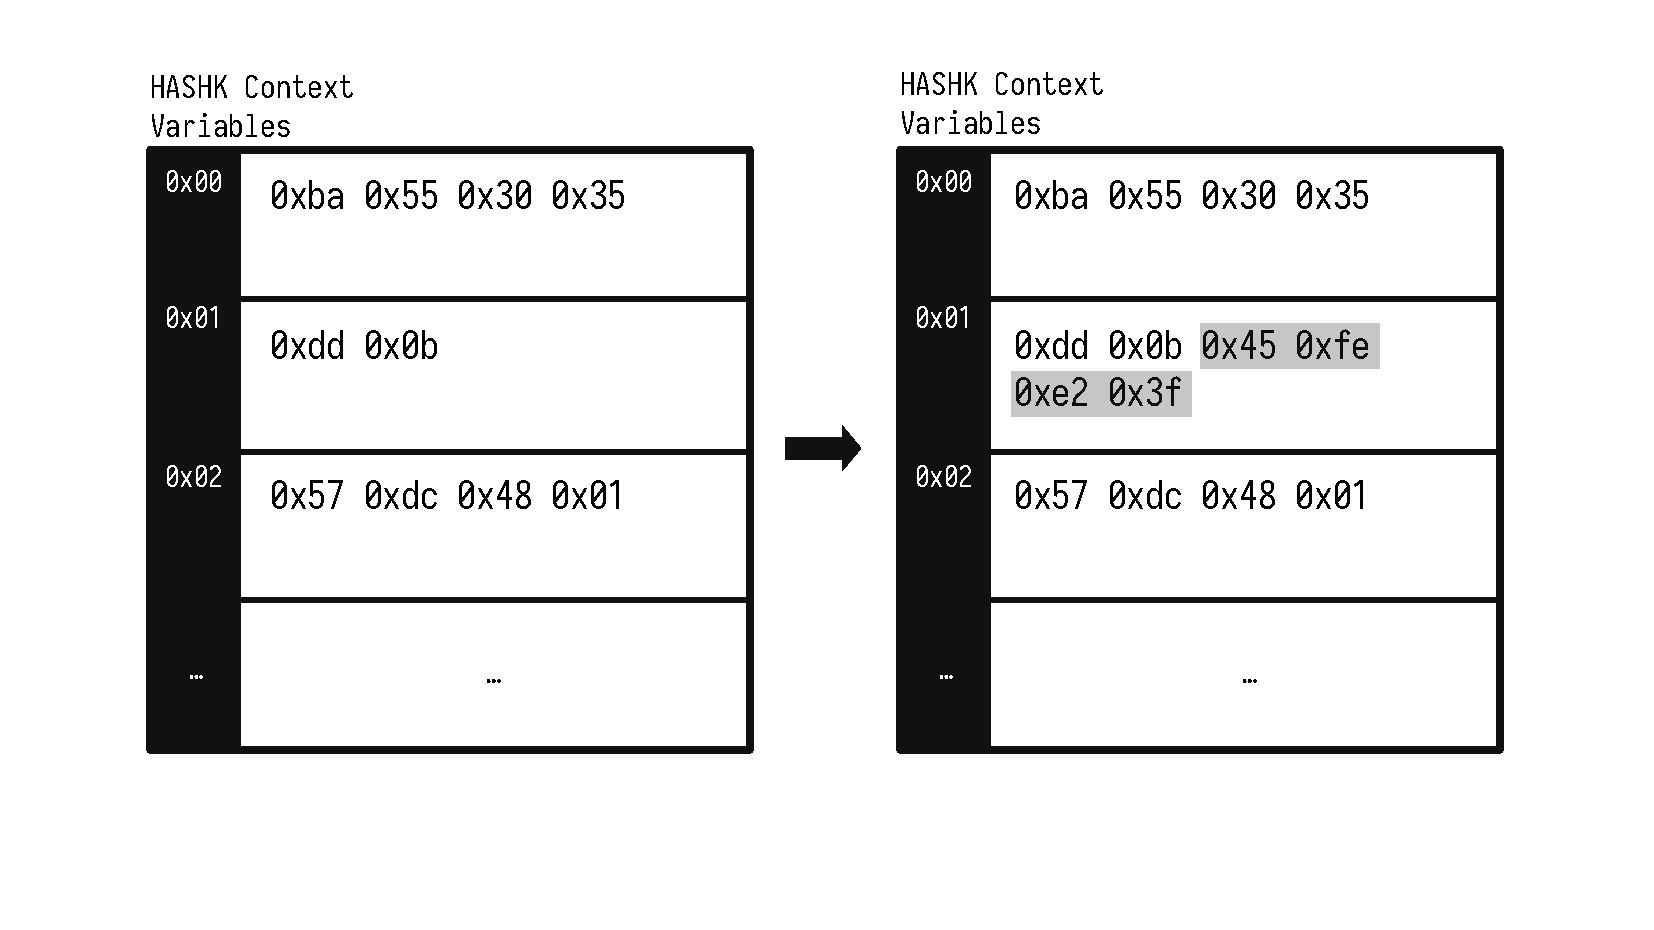
\includegraphics[width=0.6\columnwidth]{\assemblydir/figures/hashk-add-bytes}
    \caption{Schema of the \HASHK instruction.}
    \label{fig:hashk-add-bytes}
\end{figure}

The typical use of the \HASHK instruction in the zkASM language is the following one:

\begin{zkasm}
    op	:HASHK(addr)
\end{zkasm}

The \op placeholder will usually be a register or a register operation like the following one: 

\begin{zkasm}
    A + 1	:HASHK(addr)
\end{zkasm}

We can perform several hashes at the same time, each of them being stored in its corresponding address. Then, we can keep filling each of the addresses' bytes without perturbing the other ones. We can specify the address using the register \E, which is the one used to store addresses $256$-bits, or using a hard coded number. The value $0$ is usually used as an address, which is reserved for storing specific hashes. %TODO: what hashes?

\begin{zkasm}
    A + 1	:HASHK(E)
\end{zkasm}

The former instruction will append the bytes of the current value of \A + 1 into the input of the hash function we want to perform within the bytes attached to the address \E. 

To formalise what the \HASHK instruction does, let $(\op_0, \op_1, \dots, \op_{31})$ be the byte decomposition of the \op variable. We will denote $\mathtt{trunc_{D_0}}(\op)$ by the byte decomposition of \op truncated at the $\mathtt{D_0}$ position. More precisely, 
\[
\mathtt{trunc_{D_0}(\op)} = (\op_0, \op_1, \dots, \op_{\D_0-1}).
\]

Let $\mathtt{hashk}[\texttt{addr}] = (h_0, \dots, h_{\texttt{HASHPOS}})$ be the current array of bytes that we are willing to hash at a certain address \texttt{addr}. The \HASHK instruction will append the $\mathtt{trunc_{D_0}}(\op)$ array into the $\mathtt{hashk}$ one, so that the next state of the (temporal) input of the hash will become 
\[
\mathtt{hashk}[\texttt{addr}] \nextStep = (h_0, \dots, h_{\texttt{HASHPOS}}, \op_0, \op_1, \dots, \op_{\D_0-1})
\]

At the end of this operation, we increase the value of the \texttt{HASHPOS} register in $\mathtt{D_0}$:
\[
\mathtt{HASHPOS} \nextStep = \mathtt{HASHPOS} + \mathtt{D_0}.
\]

Let us propose the following simple example: suppose that we want to hash a single byte concatenated with the first $31$ bytes of a $32$-bytes integer, each of them contained in the registers $\A$ and $\B$ respectively. To that we will use the address \texttt{0x03} stored in the register \E. First of all, we should ensure that our current hash position is $0$, because we are actually starting a new hash.

\begin{zkasm}
    0x03 => E
    0 => HASHPOS
\end{zkasm}

At this moment
\[
\texttt{hashk}[\texttt{0x03}] = \emptyset.
\]

Later on, we will start adding the single byte of \A into the hash input. Observe that we should assign the length $1$ into the register \D because we need to specify the length value in bytes when using the \HASHK instruction. 

\begin{zkasm}
    1 => D
    A				:HASHK(E)
\end{zkasm}

Now, we update the array
\[
\texttt{hashk}[\texttt{0x03}] = (a)
\]
where $a$ denotes the current value of the register \A. Moreover, \texttt{HASHPOS} increased in $1$:
\[
\texttt{HASHPOS} \nextStep = \texttt{HASHPOS} + 1.
\]

Now, we do the same with the register \B

\begin{zkasm}
    31 => D
    B				:HASHK(E)
\end{zkasm}

Finally, the corresponding hash array is the following
\[
\texttt{hashk}[\texttt{0x03}] = (a, b_0, b_1, \dots, b_{30})
\]
where $(b_0, \dots, b_{30}) = \mathtt{trunc}_{31}(\B)$ are the first $31$ bytes of the register \B, which is actually the string we want to hash. Moreover, \texttt{HASHPOS} increased in $31$:
\[
\texttt{HASHPOS} \nextStep = \texttt{HASHPOS} + 31.
\]


\subsubsection{\HASHKONE}

The instruction \HASHKONE performs in the same way that \HASHK but the register $\D_0$ is not relevant here, because the size of the input string is always of $1$ byte. 


\subsubsection{\HASHKLEN}

As commented before, this instruction is actually the one that computes the hash digest and stores it internally, to later on be acquired via the \HASHKDIGEST instruction. This instruction also uses the first $32$ bytes of the \op intermediate value in order to specify the length within all the bytes stored in the specified address that will be hashed. Therefore, the total amount of bytes we can hash is $2^{32}$. 

\begin{figure}[H]
    \centering
    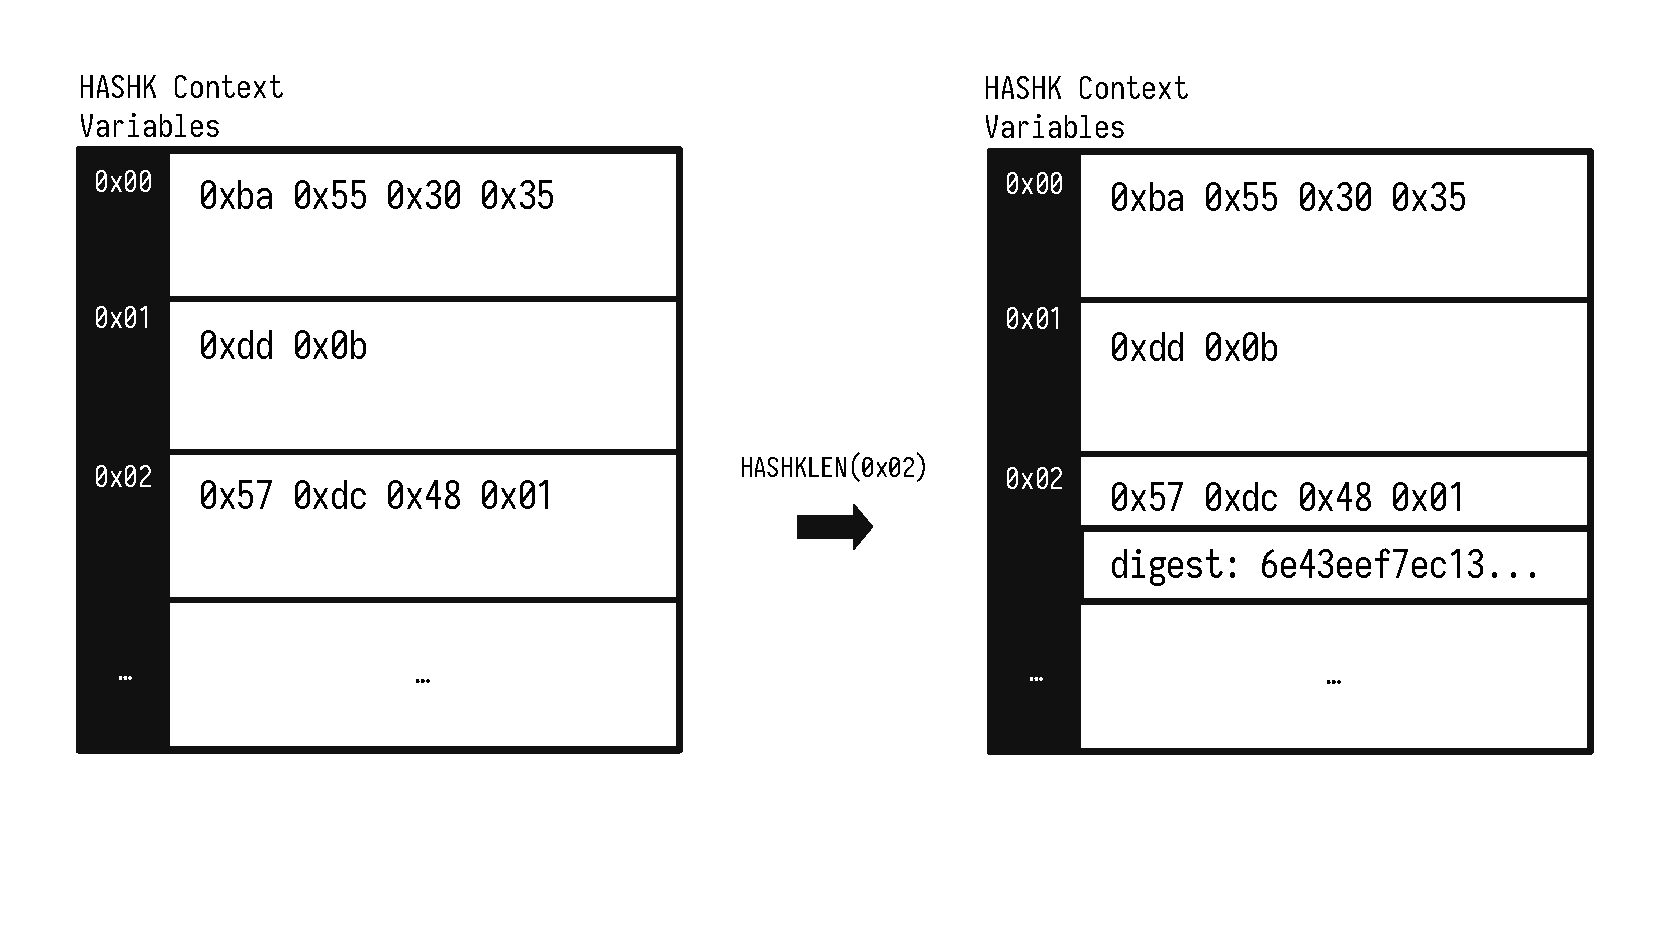
\includegraphics[width=0.6\columnwidth]{\assemblydir/figures/hashklen}
    \caption{Schema of the \HASHKLEN instruction.}
    \label{fig:hashklen}
\end{figure}


Following the previous example, the line of zkASM that we need to execute in this step is the following one:

\begin{zkasm}
    HASHPOS	:HASHKLEN(E)
\end{zkasm}

Recall that \texttt{HASHPOS} value at the current state is $32$ because we want to hash a total amount of $32$ bytes. 


More specifically, if $(h_1, \dots, h_k)$ is the input array attached to a specific address $\texttt{addr}$ (that is, $\mathtt{hashk}[\texttt{addr}] = (h_1, \dots, h_k)$ with the previous notation), the instruction

\begin{zkasm}
    len		:HASHKLEN(addr)
\end{zkasm}

internally stores the digest
\[
d = \texttt{KECCAK-256}(h_1, \dots, h_k).
\]

Observe that we should have that $k = \texttt{len}$. Otherwise, the \HASHKLEN instruction will get an error. % TODO: This checks are checking the integrity of the memory?




\subsubsection{\HASHKDIGEST}

This usual way we are invoking this instruction is the following 

\begin{zkasm}
    $ => REG	:HASHKDIGEST(E)
\end{zkasm}

Meaning that we are storing the digest of the hash attached to the address $\E$ into the register \texttt{REG}. The hash digest is introduced as a free input using the \texttt{\$ =>} operator. In our example, if we want to assign the digest of the hash to the register \D, we would use the following line

\begin{zkasm}
    $ => D		:HASHKDIGEST(E)
\end{zkasm}


%TODO: Counters needs to be incremented.





\newpage
\bibliographystyle{alpha}
\bibliography{../bib/bibliography}


\end{document}


%%%%%%%%%%%%%%%%%%%%%%%%%%%%%%%%%%%%%%%%%%%%%%%%%%%%%%%%%%%%%%%
\section{The Language}


%%%%%%%%%%%%%%%%%%%%%%%%%%%%%%%%%%%%%%%%%%%%%%%%%%%%%%%%%%%%%%%
\subsection{Introduction}

Polynomial Identity Language (PIL) is a novel domain-specific language useful for defining eAIR constraints. The aim of creating PIL is to provide developers with a holistic framework for both constructing programs through an easy-to-use interface and abstracting the complexity of the proving mechanisms.

One of the main peculiarities of PIL is its modularity, which allows programmers to define parametrizable programs, called \texttt{namespaces}, which can be instantiated from larger programs. Building programs in a modular manner makes it easier to test, review, audit and formally verify even large and complex programs. In this regard, by using PIL, developers can create their own custom namespaces or instantiate namespaces from some public library.

Many other domain-specific languages (DSL) or tool stacks, such as Circom or Halo2, focus on the abstraction of a particular computational model, such as an arithmetic circuit. However, recent proof systems such as STARKs have shown that arithmetic circuits might not be the best computational models in all use cases. Given a complete programming language, computing a valid proof for a circuit satisfiability problem, may result in long proving times due to the overhead of re-used logic. Opting for the deployment of programs, with their low-level programming, shorter proving times are attainable, especially with the advent of proof/verification-aiding languages such as PIL.









%%%%%%%%%%%%%%%%%%%%%%%%%%%%%%%%%%%%%%%%%%%%%%%%%%%%%%%%%%%%%%%
\subsection{Creating a Simple Program}\label{sec:simple-program}

To describe the fundamentals of the language itself, let us create a simple PIL program that models the computation of the product of two integers. Consider a program that, at each step, takes two input numbers and multiplies them. Naturally, this program will be referred to as the \Multiplier program. 
% It is important to recall that multiplication is defined over some (large) finite field. 
This program can be modeled using $3$ polynomials: $2$ referring to the inputs that are going to be multiplied $\freeIn_1, \freeIn_2$, and $1$ referring to the output of the computation itself $\out$. As it can be observed, the output column will exhibit a correct behavior if and only if the following identity is satisfied:
\[
\out = \freeIn_1 \cdot \freeIn_2.
\] 

A concrete example of a correct execution trace of the \Multiplier program can be seen in Figure \ref{table:multiplier-ex}. The relation above is satisfied in each of the rows of the execution trace, which means that the output column is filled with correct values. 
\begin{figure}[H]
    \centering
    \begin{tabular}{|c|}
        \hline
        \row\\ \hline
        1			\\
        2			\\
        3			\\
        4			\\
        5			\\
        6			\\
        \vdots			\\
        \hline
    \end{tabular}
    \begin{tabular}{|c|c|c|}
        \hline
        $\freeIn_1$	& $\freeIn_2$		& \out 	\\
        \hline
        4			&2				&8 		\\
        3			&1				&3 		\\
        0			&9				&0  	\\
        7			&3				&21 	\\
        4			&4				&16		\\
        5			&6				&30		\\ 
        \vdots & \vdots & \vdots \\\hline
    \end{tabular}
    \caption{An example of a valid execution trace for the \Multiplier program.}
    \label{table:multiplier-ex}
\end{figure}

%TODO: I think the following is not correct
As it can be seen, there exists a noticeable difference between the behavior of the input columns and the output column which suggests the following classification,
\begin{itemize}
    \item \textbf{Free Input Polynomials:} These are columns that are in charge of introducing the various inputs to the computation. They are referred to as ``free" because at every clocking of the computation, their values do not strictly depend on any previous iteration. These are analogous to independent variables of the entire computation.
    
    \item \textbf{State Variables:} These are the columns that compose the state of the program. Here state refers to the set of values that represent the output of the program at each step and, if we are in the last step, the output of the entire computation.
\end{itemize}




We can now write the corresponding PIL program for the \Multiplier program:
\begin{pil}
    namespace Multiplier(2**10);
    
    // Polynomials
    pol commit freeIn1;
    pol commit freeIn2;
    pol commit out;
    
    // Constraints
    out = freeIn1*freeIn2;
\end{pil}

The reserved keyword \texttt{namespace} is used to frame the scope of the program definition. Inside it, one should define the polynomials used by its program and the constraints among the defined polynomials. A namespace has to be instantiated with a unique name (\Multiplier) together with an argument representing the length of the program, that is, the number of rows (in this case, $2^{10}$) of any execution trace of that program. Besides, the \texttt{commit} keyword allows the compiler to identify the corresponding polynomial as \textbf{committed}. Committed polynomials are opposed to \textbf{constant} polynomials, which are polynomials that are not allowed to change among any execution of the same program. That is, constant polynomials are inherent to the computation itself. This is important from the proving perspective since constant polynomials are publicly known by all parties. However, this is not the case for committed polynomials, which are, in most cases, only known by a party. More on constant polynomials will be added below. 

One should observe that, of course, the former design of the \Multiplier program is not unique. This design is highly not scalable to more complex operations since the number of committed polynomials grows linearly with the number of operations we want to perform. For example, designing a program that computes the result of performing $2^{10}$ operations following the previous design would require $2^{10}$ committed polynomials, which is far from being practical.

However, following another design strategy can easily reduce the $2^{10}$ committed polynomials to a single one by the introduction of another polynomial that flags the starting row of each operation. Together with a third polynomial holding the result of the operation, only a total amount of $3$ columns will be needed. Returning to the initial \Multiplier program, the idea is to introduce a \textbf{constant} polynomial called \RESET that will evaluate to $1$ in odd rows and $0$ otherwise (see Figure \ref{table:multiplier-ex-with-flag}). Nonetheless, this design will also decrease the number of multiplications that can be checked given the same number of rows as the initial design. More concretely, using the initial design we can check one multiplication per row, meanwhile adopting this new strategy will half the number of possible multiplication. 

\begin{figure}[H]
    \centering
    \begin{tabular}{|c|}
        \hline
        \row\\ \hline
        1			\\
        2			\\
        3			\\
        4			\\
        5			\\
        6			\\
        7			\\
        \vdots			\\
        \hline
    \end{tabular}
    \begin{tabular}{|c|c|c|}
        \hline
        \freeIn	&\RESET		&\out 	\\
        \hline
        \textcolor{red}{4}			&1				&0 		\\
        \textcolor{red}{2}			&0				&4 		\\
        \textcolor{orange}{3}			&1				&\textcolor{red}{8}  	\\
        \textcolor{orange}{1}			&0				&3 		\\
        \textcolor{blue}{9}			&1				&\textcolor{orange}{3}		\\
        \textcolor{blue}{0}			&0				&0		\\
        0			&1				&\textcolor{blue}{0}		\\
        \vdots	&\vdots		&\vdots \\ \hline
    \end{tabular}
    \caption{An example of a valid execution trace for the new design of the \texttt{Multiplier} program.}
    \label{table:multiplier-ex-with-flag}
\end{figure}

Observe that, whenever \RESET equals $1$, the value of the \texttt{out} polynomial equals the result of multiplying the previous two values of the \texttt{freeIn} polynomial. In the intermediate steps (that is, when \RESET is equal to $0$), the \texttt{out} polynomial stores the first input of the multiplication. 

Of course, we need to adapt the \Multiplier constraint to reflect the correctness of the \texttt{out} polynomial to the new design. One can observe the following constraint:
\[
\nextStep{\out} = \RESET \cdot \freeIn + (1 - \RESET) \cdot (\out \cdot \freeIn)
\]
completely describes the new design. In PIL, a tick \nextStep{} (which is read ``prime'') over a polynomial is used to denote the value in the next row of such polynomial. In the case of polynomials defined over a multiplicative subgroup $G$ of a prime field $\FF$ with generator $g$, the prime notation is equivalent to the polynomial $\nextStep{\out}(X):= \out(Xg)$.

To see that the previous constraint completely describes our new \Multiplier design, let us distinguish between two cases: 
\begin{itemize}
    \item When \RESET is equal to $1$, the above constraint becomes:
    \[
    \nextStep{\out} = \freeIn.
    \]
    Hence, we are setting the \freeIn polynomial's value in the current row into the \out polynomial's value of the next row.
    
    \item When \RESET is equal to $0$, the above constraint becomes:
    \[
    \nextStep{\out} = \out \cdot \freeIn.
    \]
    Hence, this constraint is stating that the \out polynomial's value in the next row will become the product of the value of \freeIn in the last two rows, the more distance contained in the \out polynomial (as in PIL we are not allowed to access to more than one previous row's values). 
\end{itemize}

The optimized design of the \Multiplier program can be written in PIL as follows:
\begin{pil}
    namespace Multiplier(2**10);
    
    // Constant Polynomials
    pol constant RESET;
    
    // Committed Polynomials
    pol commit freeIn;
    pol commit out;
    
    // Constraints
    out' = RESET*freeIn + (1-RESET)*(out*freeIn);
\end{pil}
Observe that now, the polynomial \RESET is defined with the reserved keyword \texttt{constant}, because it does not change among several executions of the same program. Finally, note that the same design can be extended for a much larger amount of multiplications without needing to modify the PIL itself. Instead, we simply would extend the \RESET polynomial as follows:
\[
\RESET = 
\begin{cases}
    1, & \text{if } i \equiv 0 \pmod{n} \\
    0, & \text{otherwise}
\end{cases}
\]
where $i$ represents the row number (starting from $0$) and $n$ refers to the number of operations.




%%%%%%%%%%%%%%%%%%%%%%%%%%%%%%%%%%%%%%%%%%%%%%%%%%%%%%%%%%%%%%%
\subsection{Compilation}

The previous PIL program is almost ready to be compiled into a JSON file using the \pilcom package \cite{pilcom}. This file is a basic JSON representation of the PIL program (with some extra metadata) that will be consumed later on by the \texttt{pil-stark} package \cite{pilstark} to generate a STARK proof. However, there is a strong restriction when dealing with PIL's constraints. Let $S$ be the set of all polynomials defined over a field $\FF$ appearing in the PIL program. Formally, a constraint is a polynomial identity $f = 0$ where $f \in \FF[S, \nextStep{S}]$ where $\nextStep{S}$ is the set of all the shifted polynomials $p(g X)$ with $p \in S$. The restriction in PIL is the following: \textbf{the degree of $f$ must be less or equal to $2$}.

For example, recall the previous PIL program for the optimized \Multiplier program. The constraint 
\[
\nextStep{\out} = \RESET \cdot \freeIn + (1 - \RESET) \cdot (\out \cdot \freeIn).
\]
can be viewed as the polynomial identity $f = 0$ where $f$ equals to
\[
\nextStep{\out} - \RESET \cdot \freeIn + (1 - \RESET) \cdot (\out \cdot \freeIn)
\]
which belongs to $\FF[\out, \nextStep{\out}, \RESET, \freeIn]$ but \textbf{does not have degree less or equal than $2$}, because it contains the monomial
\[
\RESET \cdot \out \cdot \freeIn.
\]

The idea that PIL has introduced to solve this limitation is to create a new polynomial, conveniently named \texttt{carry}, that will store the product $\out \cdot \freeIn$, that is,
\[
\carry = \out \cdot \freeIn.
\]

This kind of polynomial will be called \textbf{intermediate}. Observe that the prover does not need to provide intermediate polynomials since they can be derived directly from the committed and constant polynomials. Only the way of computing it is strictly necessary. 

Now, the former PIL program can be modified to introduce this newly intermediate \texttt{carry} polynomial:
\begin{pil}
    namespace Multiplier(2**10);
    
    // Constant Polynomials
    pol constant RESET;
    
    // Committed Polynomials
    pol commit freeIn;
    pol commit out;
    
    // Intermediate Polynomials
    pol carry = out*freeIn;
    
    // Constraints
    out' = RESET*freeIn + (1-RESET)*carry;
\end{pil}

At this point, given a (valid) PIL file (ending with the \texttt{.pil} extension) the \pilcom compiler will return a JSON file. %TODO: Add the JSON in the appendix
For example, the \Multiplier program's PIL located in \texttt{multiplier.pil} can be compiled by invoking the following command:

\begin{lstlisting}
    pilcom$ node src/pil.js multiplier.pil -o multiplier.json
\end{lstlisting}

Apart from the JSON file, the compiler will throw a debugging message into the console:

\begin{lstlisting}
    Input Pol Commitments: 2
    Q Pol Commitmets: 1
    Constant Pols: 1
    Im Pols: 1
    plookupIdentities: 0
    permutationIdentities: 0
    connectionIdentities: 0
    polIdentities: 1
\end{lstlisting}

In the previous message, it can be checked that the number of committed polynomials (\texttt{Input Pol Commitments}), the number of constant polynomials (\texttt{Constant Pols}), the number of intermediate polynomials (\texttt{Im Pols}) and the total number of identity constraints (\texttt{polIdentities}) agrees with the corresponding PIL code. 



%TODO: I think we should move this to the connection programs section
Since one of the key features of PIL is that it allows modularity, a dependency inclusion feature among different \texttt{.pil} files have been developed. To briefly show this feature, a configuration \texttt{.pil} file containing the degree bound for polynomials will be created and be used along several PIL programs to remove magic numbers like $2^{10}$. More generically, \texttt{config.pil} will typically include some configuration-related components, shared among various programs. To declare a constant, it can do it using the \texttt{constant} keyword. The compiler distinguishes between constants identifiers and other identifiers (like polynomial identifiers) via the percent \texttt{\%} symbol. Henceforth, constant identifiers should be preceded by the percent symbol. 

\begin{pil}
    // Filename: config.pil
    
    constant %N = 2**10;
\end{pil}

In order to relate both files, the \texttt{include} reserved keyword must be invoked.

\begin{pil}
    // Filename: multiplier.pil
    
    include "config.pil";
    
    namespace Multiplier(%N);
    
    // Constant Polynomials
    pol constant RESET;
    
    // Committed Polynomials
    pol commit freeIn;
    pol commit out;
    
    // Intermediate Polynomials
    pol carry = out*freeIn;
    
    // Constraints
    out' = RESET*freeIn + (1-RESET)*carry;
\end{pil}








%TODO: I think that we can remove this section
%%%%%%%%%%%%%%%%%%%%%%%%%%%%%%%%%%%%%%%%%%%%%%%%%%%%%%%%%%%%%%%
%\subsection{Compiling a Machine (degree 3)}
%
%Suppose now that we are willing to modify the previous program in order not to compute simple multiplications $x \cdot y$ for $x, y \in \FF$ but squared multiplications $x^2 \cdot y^2$. We will call this program \textit{SquareAndMultiply} program. We can model this computation in the same way as before, but modifying the PIL accordingly:
%
%\begin{figure}[H]
%\centering
%\[
%\begin{array}{|c|c|c|}
%\hline
%\freeIn	&\RESET		&\out 	\\
%\hline
%4			&1				&0 		\\
%2			&0				&16		\\
%3			&1				&64  	\\
%1			&0				&9 		\\
%9			&1				&9		\\
%0			&0				&81		\\
%\dots		&\dots			&\dots \\ \hline
%\end{array}
%\]
%\caption{Concrete example of a correct execution of the \texttt{SquareAndMultiply} program.}
%\label{table:multiplier-ex-with-flag2}
%\end{figure}
%
%\begin{pil}
%namespace Multiplier(2**10);
%
%    // Constant Polynomials
%    pol constant RESET;
%
%    // Input Polynomials
%    pol commit freeIn;
%
%    // State Variables
%    pol commit out;
%
%    // Constraints
%    out' = RESET*freeIn*freeIn + (1 - RESET)*(out*freeIn*freeIn);
%\end{pil}
%
%The previous PIL program is almost ready to be compiled into a \texttt{.json} that can be interpreted by the \pilcom package %TODO: Link package
%in order to generate a valid set of polynomials and constraints, which will be used later on by the \texttt{pil-stark} package to generate a valid proof. However, there is a strong restriction when dealing with PIL's constraints. Let $S$ be the set of all polynomials (or equivalently, columns) defined over a field $\FF$ appearing in the PIL program. Formally, a constraint is a polynomial identity $f = 0$ where $f \in \FF[S, \nextStep{S}]$ where $\nextStep{S}$ is the set of all the shifted polynomials $p(g X)$ with $p \in S$. The restriction in PIL is the following: \textbf{the degree of $f$ must be less or equal than $3$}.
%
%For example, recall the previous PIL program for the optimized \Multiplier program. The constraint 
%\[
%    \nextStep{\out} = \RESET \cdot \freeIn \cdot \freeIn + (1 - \RESET) \cdot (\out \cdot \freeIn \cdot \freeIn).
%\]
%can be viewed as the polynomial identity $f = 0$ where $f$ equals to
%\[
%    \nextStep{\out} - \RESET \cdot \freeIn \cdot \freeIn + (1 - \RESET) \cdot (\out \cdot \freeIn \cdot \freeIn)
%\]
%which belongs to $\FF[\out, \nextStep{\out}, \RESET, \freeIn]$ but \textbf{does not have degree less or equal than $3$}, because it contains the monomial
%\[
%\RESET \cdot \out \cdot \freeIn \cdot \freeIn.
%\]
%
%The idea that PIL has introduced to solve this limitation is to create a new polynomial, conveniently named \texttt{square}, that will store the product $\freeIn \cdot \freeIn$, that is,
%\[
%\texttt{square} = \freeIn \cdot \freeIn.
%\]
%
%This kind of polynomials will be called \textbf{intermediate}. Observe that the prover does not need to provide intermediate polynomials since they can be derived directly from the committed and constant polynomials. Only the way of computing is strictly necessary. 
%
%Now, the former PIL program can be modified in order to introduce this newly intermediate \texttt{square} polynomial:
%
%\begin{pil}
%namespace Multiplier(2**10);
%
%    // Constant Polynomials
%    pol constant RESET;
%
%    // Input Polynomials
%    pol commit freeIn;
%
%    // State Variables
%    pol commit out;
%
%    // intermediate Polynomials
%    pol square = freeIn*freeIn;
%
%    // Constraints
%    out' = RESET*square + (1 - RESET)*out*square;
%\end{pil}
%
%At this point, given a (valid) PIL file (ending with the \texttt{.pil} extension) the \pilcom compiler will return a \texttt{.json} file. For example, the Multiplier program's PIL located in \texttt{multiplier.pil} can be compiled by invoking the following command:
%
%\begin{lstlisting}
%pilcom$ node src/pil.js multiplier.pil -o <output.pil.json>
%\end{lstlisting}
%
%Apart from the \texttt{.json} file, the compiler will throw a debugging message into the console:
%
%\begin{lstlisting}
%Input Pol Commitments: 2
%Q Pol Commitmets: 1
%Constant Pols: 1
%Im Pols: 1
%plookupIdentities: 0
%permutationIdentities: 0
%connectionIdentities: 0
%polIdentities: 1
%\end{lstlisting}
%
%In the previous message it can be checked the number of committed polynomials (\texttt{Input Pol Commitments}), the number of constant polynomials (\texttt{Constant Pols}), the number of intermediate polynomials (\texttt{Im Pols}) and the total number of polynomial constraints (\texttt{polIdentities}) used in the compiled PIL code. 
%
%Since one of the key features of PIL is that is allows modularity, a dependency inclusion feature among different \texttt{.pil} files has been developed. In order to briefly show this feature, a configuration \texttt{.pil} file containing the degree bound for polynomials will be created and be used along several PIL programs to remove magic numbers like $2^{10}$. More generically, \texttt{config.pil} will typically include some configuration-related components, shared among various programs. To declare a constant, it can be do it using the \texttt{constant} keyword. The compiler distinguish between constants identifiers and other identifiers (like polynomial identifiers) via the percent \texttt{\%} symbol. Henceforth, constant identifiers should be preceded by the percent symbol. 
%
%\begin{pil}
%// Filename: config.pil
%
%constant %N = 2**10;
%\end{pil}
%
%In order to relate both files, the \texttt{include} reserved keyword must be invoked.
%
%\begin{pil}
%// Filename: multiplier.pil
%
%include "config.pil";
%
%namespace Multiplier(%N);
%
%    pol constant RESET;
%    pol commit freeIn;
%    pol commit out;
%    pol square = freeIn*freeIn;
%    
%    out' = RESET*square + (1 - RESET)*out*square;
%\end{pil}







%%%%%%%%%%%%%%%%%%%%%%%%%%%%%%%%%%%%%%%%%%%%%%%%%%%%%%%%%%%%%%%
\subsection{Cyclic Constraints}

Since execution traces have finite length $N$, there is one implicit complexity in the design of programs with PIL: constraints should be satisfied over every element of a subgroup $G = \Angle{g}$ of $\FF^*$ of size $N$. This means that the description (in terms of constraints) of a program is not correct if the appropriate constraints are not satisfied in every row transition. This is because the polynomials defined from the columns of the execution trace are constructed by interpolation at $G$. In particular, constraints containing polynomials using the prime notation should remain true in the transition from the last row to the first row because $g \cdot g^{N} = g \cdot 1 = g$ (by Lagrange's theorem) and therefore:
\[
\nextStep{p}(g^{N}) = p(g \cdot g^N) = p(g),
\]
which is the first value of the column defined by the polynomial $p$. 

This is an important aspect that has to be taken care of when designing the set of constraints of a program with PIL. If there is some constraint that is not satisfied in the last transition, one normally overcomes this problem by the inclusion of additional polynomials that solve this issue. For example, consider the following PIL code:
\begin{pil}
    namespace CyclicExample(4);
    pol commit a, b;
    
    (a+1)*a*(a-1) = 0;
    b' = b+a;
\end{pil}
and the following valid execution trace:
\begin{figure}[H]
    \centering
    \begin{tabular}{|c|}
        \hline
        \row\\ \hline
        1			\\
        2			\\
        3			\\
        4			\\
        \hline
    \end{tabular}
    \begin{tabular}{|c|c|}
        \hline
        \att	&\btt \\ \hline
        1			&1			\\
        0			&2			\\
        -1			&2			\\
        1			&1			\\
        \hline
    \end{tabular}
\end{figure}

Observe that the polynomial \att only takes the values $0, 1$ or $-1$ (equivalently, $p-1$) and this is precisely captured by the constraint: 
\[
(\att+1) \cdot \att \cdot (\att-1) = 0,
\]
which is satisfied for each row $i \in [4]$.

On the other side, the second constraint $\nextStep{\btt} = \btt + \att$ is satisfied for every row except for the last, because: 
\begin{equation}\label{eq:cyclic}
    \nextStep{\btt}(g^4) = \btt(1) = 1 \neq 2 = 1 + 1 = \btt(g^4) + \att(g^4),
\end{equation}
where $g$ is the generator of the group $G$ of size $4$.

The idea to overcome this problem is to add a constant column \SEL that is $1$ in every row except for the last one and introduce it to the previous constraint as follows:
\[
\btt' = \SEL \cdot (\btt+\att) + (1-\SEL).
\]
Notice that now the right-hand side of Eq. \eqref{eq:cyclic} is equal to $\SEL(g^4) \cdot (\btt(g^4) + \att(g^4)) + (1-\SEL(g^4)) = 1$.

The valid PIL is the following:
\begin{pil}
    namespace CyclicExample(4);
    
    pol commit a, b;
    pol constant SEL;
    pol carry = (a+1)*a;
    
    carry*(a-1) = 0;
    b' = SEL*(b+a) + (1-SEL);
\end{pil}








%%%%%%%%%%%%%%%%%%%%%%%%%%%%%%%%%%%%%%%%%%%%%%%%%%%%%%%%%%%%%%%
\subsection{Inclusion Arguments}

There is a subtlety in the \Multiplier example of Section \ref{sec:simple-program} that is worth commenting on at this point. It is assumed that columns can contain field elements but, it may be the case where one needs to restrict the size of the columns' values to a certain number of bits. Henceforth, it is important to develop a strategy to control both underflows and overflows. In this section, we will design a program (and its corresponding PIL) to verify the addition of two integers of a size fitting in exactly $2$ bytes. That is, any input to the addition will be considered invalid if it is not an integer in the range $[0,65535]$.

Of course, there is plenty of ways to arithmetize this program. However, in this section, we are going to use a method based on inclusion arguments. The overall idea is to reduce $2$-byte additions to $1$-byte additions. Specifically, the program will consist of two input polynomials \att and \btt where each one will, at each row, introduce a single byte (equivalently, an integer in the range $[0,255]$) for each operand of the sum, starting with the less significant byte. Hence, every two rows, a new addition will be checked.
\begin{figure}[H]
    \centering
    \begin{tabular}{|c|}
        \hline
        \row\\ \hline
        1			\\
        2			\\
        3			\\
        4			\\
        \hline
    \end{tabular}
    \begin{tabular}{|c|c|c|}
        \hline
        \att		&\btt		& \texttt{operation} \\
        \hline
        \texttt{0x11}	&\texttt{0x22}	&\textit{undefined}\\
        \texttt{0x30}	&\texttt{0x40}	&\texttt{0x3011} + \texttt{0x4022}\\
        \texttt{0xff}	&\texttt{0xee}	&\textit{undefined}\\
        \texttt{0x00}	&\texttt{0xff}	&\texttt{0x00ff} + \texttt{0xffee}\\
        \hline
    \end{tabular}
    \label{table:2-bytes-sum-sm}
\end{figure}

The output of the addition between words of $1$-byte can not be stored in a single column that only accepts words of $1$-byte, since an overflow may appear. Hence, the result of the addition will be split into two columns \texttt{carry} and \add, accepting words of exactly $1$-byte, to completely store the result so that a correct addition between bytes can be defined as:
\begin{equation}
    \label{byte-sum-carry}
    \att + \btt = \carry \cdot 2^8 + \add.
\end{equation}

Table \ref{table:2-bytes-sum-carry-add} shows an example of a valid execution trace for this program. Note that the result of operating each of the $2$-bytes words can be obtained by simply grabbing the value in the last \texttt{carry} value and each of the last two \add's values in decreasing order. For example, $\mathtt{0x3011} + \mathtt{0x4022} = \mathtt{0x007033}$, which can be recovered from the blue cells below. The same applies for $\mathtt{0x00ff} + \mathtt{0xffee} = \mathtt{0x0100ed}$, which can be recovered similarly from the pink cells. 

\begin{table}[H]
    \centering
    \begin{tabular}{|c|}
        \hline
        \row\\ \hline
        1			\\
        2			\\
        3			\\
        4			\\
        \hline
    \end{tabular}
    \begin{tabular}{|c|c|c|c|}
        \hline
        \att		&\btt		&\carry		&\add 	\\
        \hline
        \texttt{0x11}	&\texttt{0x22}	&\texttt{0x00}		&\cellcolor{cyan} \texttt{0x33} 	\\
        \texttt{0x30}	&\texttt{0x40}	&\cellcolor{cyan} \texttt{0x00}		&\cellcolor{cyan} \texttt{0x70}	\\ \hline
        \texttt{0xff}	&\texttt{0xee}	&\texttt{0x01}		&\cellcolor{pink} \texttt{0xed}  \\
        \texttt{0x00}	&\texttt{0xff}	&\cellcolor{pink} \texttt{0x01}		&\cellcolor{pink} \texttt{0x00}	\\
        \hline
    \end{tabular}
    \caption{TBD}
    \label{table:2-bytes-sum-carry-add}
\end{table}

One can notice that constraint \eqref{byte-sum-carry} is not satisfied at row $4$, because the \carry's value that is raised in the third row must be introduced into the $1$-byte addition at row $4$. In this way, we can link the two-byte sums that compose $2$-byte additions. There is no direct way to introduce the previous row of a column in PIL (in contrast with the next row, which we can invoke with the single quote operator \nextStep{}). The idea then is to introduce another committed polynomial called \texttt{prevCarry} which will contain a shifted version of the value in the  \texttt{carry} polynomial. More specifically, we add the following constraint to ensure that \texttt{prevCarry} is correctly defined:
\begin{equation}\label{eq:carries}
    \mathtt{prevCarry}' = \carry
\end{equation}

\begin{figure}[H]
    \centering
    \begin{tabular}{|c|}
        \hline
        \row\\ \hline
        1			\\
        2			\\
        3			\\
        4			\\
        \hline
    \end{tabular}
    \begin{tabular}{|c|c|c|c|c|}
        \hline
        \att		&\btt		&\texttt{prevCarry}		&\carry	&\add 	\\
        \hline
        \texttt{0x11}	&\texttt{0x22}	&\texttt{0x01}		&\texttt{0x00}		&\texttt{0x33} 	\\
        \texttt{0x30}	&\texttt{0x40}	&\texttt{0x00}		&\texttt{0x00}		&\texttt{0x70}	\\ \hline
        \texttt{0xff}	&\texttt{0xee}	&\texttt{0x00}		&\texttt{0x01}		&\texttt{0xed}  \\
        \texttt{0x00}	&\texttt{0xff}	&\texttt{0x01}		&\texttt{0x01}		&\texttt{0x00}	\\
        \hline
    \end{tabular}
    \label{table:2-bytes-sum-prev-carry}
\end{figure}

Now we face another problem: the previous carry must not affect two different 2-byte additions as per constraint \eqref{eq:carries}. That is, non-related operations should not be linked via carries. Henceforth, a constant polynomial called \RESET will be introduced to break the present connection between different additions. The \RESET polynomial will be a binary-ranged polynomial which will be $1$ at the beginning of every $2$ byte addition. Elsewhere, \RESET will evaluate to $0$. 

\begin{figure}[H]
    \centering
    \begin{tabular}{|c|}
        \hline
        \row\\ \hline
        1			\\
        2			\\
        3			\\
        4			\\
        \hline
    \end{tabular}
    \begin{tabular}{|c|c|c|c|c|c|c}
        \hline
        \att		&\btt		&\texttt{prevCarry}	&\carry		&\add		&\RESET 	\\
        \hline
        \texttt{0x11}	&\texttt{0x22}	&\texttt{0x01}		&\texttt{0x00}		&\texttt{0x33}		&1 					\\
        \texttt{0x30}	&\texttt{0x40}	&\texttt{0x00}		&\texttt{0x00}		&\texttt{0x70}		&0					\\ \hline
        \texttt{0xff}	&\texttt{0xee}	&\texttt{0x00}		&\texttt{0x01}		&\texttt{0xed}		&1  				\\
        \texttt{0x00}	&\texttt{0xff}	&\texttt{0x01}		&\texttt{0x01}		&\texttt{0x00}		&0					\\
        \hline
    \end{tabular}
    \label{table:2-bytes-sum-reset}
\end{figure}

Following this logic, we can now derive the final (and accurate) constraint: 
\begin{equation}
    \label{byte-sum-pil}
    \att + \btt + (1 - \RESET) \cdot \mathtt{prevCarry} = \carry \cdot 2^8 + \add.
\end{equation}

The PIL program of the previous example can be written as follows:
\begin{pil}
    include "config.pil";
    
    namespace TwoByteAdd(%N);
    
    pol constant RESET;
    pol commit a, b;
    pol commit carry, prevCarry, add;
    
    prevCarry' = carry;
    a + b + (1-RESET)*prevCarry = carry*2**8 + add;
\end{pil}

% Observe that the constraint $(1 - \RESET)\cdot\RESET = 0$ has been added in order to enforce \RESET to be binary. 
Similarly to the \Multiplier example of Section \ref{sec:simple-program}, it is worth mentioning that only by changing the \RESET polynomial (but not the PIL itself), it is possible to arithmetize a program being able to verify generic $n$-bytes additions. In such case, \RESET will be $1$ for every $n$ row and $0$ otherwise. 

Up to this point, one can think that Constraint \eqref{byte-sum-pil} restricts a sound representation of the program. However, since we are working over a finite field, it is not. For example, the following execution trace is valid, as it satisfies all the constraints, but does not correspond to a valid computation:
\begin{figure}[H]
    \centering
    \begin{tabular}{|c|}
        \hline
        \row\\ \hline
        1			\\
        2			\\
        3			\\
        4			\\
        \hline
    \end{tabular}
    \begin{tabular}{|c|c|c|c|c|c|c}
        \hline
        \att		&\btt		&\texttt{prevCarry}					&\carry		&\add								&\RESET 	\\
        \hline
        \texttt{0x11}	&\texttt{0x22}	&\texttt{0x01}						&$p \cdot 2^{-8}$					&\texttt{0x33}					&1 					\\
        \texttt{0x30}	&\texttt{0x40}	&$p \cdot 2^{-8}$						&\texttt{0x00}					&$\texttt{0x70} + p \cdot 2^{-8}$	&0					\\ \hline
        \texttt{0xff}	&\texttt{0xee}	&\texttt{0x00}						&$\texttt{0x01} + p \cdot 2^{-8}$	&\texttt{0xed}					&1  				\\
        \texttt{0x00}	&\texttt{0xff}	&$\texttt{0x01} + p \cdot 2^{-8}$		&\texttt{0x01}					&$\texttt{0x00}+ p \cdot 2^{-8}$	&0					\\
        \hline
    \end{tabular}
    \caption{Concrete example showing how to cheat the current program restrictions. }
    \label{table:2-bytes-sum-wrong}
\end{figure}

Moreover, nothing is preventing the introduction of more bytes in either column \a or \b, which breaks the intention of this program, specially designed to deal only with byte-sized columns. Enforcing that all the evaluations of committed polynomials are correct is strictly necessary. As explained at the beginning of this section, an inclusion argument will be used.  

\begin{definition}[Inclusion Argument]
    Given two vectors $a = (a_1, \dots, a_n) \in \FF_p^n$ and $b = (b_1, \dots, b_m) \in \FF_p^m$, we say that \textit{$a$ is contained in $b$} if for all $i \in [n]$, there exists a $j \in [m]$ such that $a_i = b_j$. In words, if we see $a$ and $b$ as multisets and then we reduce them to sets (by removing the multiplicity), then $a$ is contained in $b$ if $a$ is a subset of $b$.
    
    Moreover, we say that a protocol $(\P,\V)$ is an \textit{inclusion argument} if the protocol can be used by $\P$ to prove to $\V$ that one vector is contained in another vector.
\end{definition}

% An inclusion argument is a constraint defined in PIL that is used to check whether $\att \subset \btt$ where \att and \btt are two columns. Since polynomials can be described as vectors via the usual Fourier transform procedure, the following definition can be naturally extended to columns. It is important to observe that $n$ can be less, equal or bigger than $m$ and the former definition still makes sense. Later on, a more restrictive constraint will be introduced.

In the PIL context, the implemented inclusion argument is the inclusion argument provided here \cite{EPRINT:GabWil20}, with the ``alternating method''  provided in \cite{EPRINT:PFMBM22} and can be invoked via the \textsf{in} keyword. Specifically, given two columns \att, \btt, we can declare an inclusion argument between them using the syntax $\{\att\} \textsf{ in } \{\btt\}$, where \att, \btt does not necessarily need to be defined in different programs. See for example:
\begin{pil}
    include "config.pil";
    
    namespace A(%N);
    pol commit a, b;
    
    {a} in {b};
    
    namespace B(%N);
    pol commit a, b;
    
    {a} in {Example1.b};
\end{pil}
A valid execution trace (with $N=4$) for the previous example is shown in Table \ref{table:is-example-1}.
\begin{table}[H]
    \centering
    \begin{tabular}{|c|c|}
        \hline
        \multicolumn{2}{|c|}{\textbf{Program A}} \\
        \hline
        \att	&\btt	\\ \hline
        3	&1	\\
        4	&2 \\
        2	&3\\
        3	&4 \\
        \hline
    \end{tabular}
    \begin{tabular}{|c|c|}
        \hline
        \multicolumn{2}{|c|}{\textbf{Program B}} \\
        \hline
        \att	&\btt	\\ \hline
        1	&6 \\
        1	&7 \\
        1	&8 \\
        4	&9 \\
        \hline
    \end{tabular}
    \caption{Execution traces for programs \textsf{A} and \textsf{B}. }
    \label{table:is-example-1}
\end{table}

In PIL we can also write inclusion arguments not only over single columns but over multiple columns. That is, given two subsets of committed columns $\att_1,\dots,\att_m$ and $\btt_1,\dots,\btt_m$ of some program(s) we can write $\{\att_1,\dots,\att_m\} \texttt{ in } \{\btt_m,\dots,\btt_m\}$ to denote that the rows generated by columns $\btt_m,\dots,\btt_m$ are included (as sets) into the rows generated by columns $\{\att_1,\dots,\att_m\}$. A natural application for this generalization is showing that a set of columns in a program repeatedly computes, probably with the same pair of inputs/outputs, an operation such as $\AND$, where the correct $\AND$ operation is carried on a distinct program (see the following example).
\begin{pil}
    include "config.pil";
    
    namespace Main(%N);
    pol commit a, b, c;
    
    {a,b,c} in {in1,in2,xor};
    
    namespace AND(%N);
    pol constant in1, in2, and;
\end{pil}

%TODO: We should mention that we can add selectors

Following with the previous example, the idea will be to construct $4$ new constant polynomials $\mathtt{BYTE\_A}$, $\mathtt{BYTE\_B}$, $\mathtt{BYTE\_CARRY}$ and $\mathtt{BYTE\_ADD}$ which contain all possible byte additions. The execution trace of these polynomials can be constructed as follows:
\begin{figure}[H]
    \centering
    \begin{tabular}{|c|}
        \hline
        \row\\ \hline
        1			\\
        2			\\
        3			\\
        \vdots			\\
        256			\\
        257			\\
        258			\\
        \vdots			\\
        65535		\\
        65536			\\
        \hline
    \end{tabular}
    \begin{tabular}{|c|c|c|c|}
        \hline
        \texttt{BYTE\_A}	&\texttt{BYTE\_B}	&\texttt{BYTE\_{CARRY}}	&\texttt{BYTE\_{ADD}} \\
        \hline
        \texttt{0x00}		&\texttt{0x00}		&\texttt{0x00}			&\texttt{0x00}		  \\
        \texttt{0x00}		&\texttt{0x01}		&\texttt{0x00}			&\texttt{0x01}		  \\
        \texttt{0x00}		&\texttt{0x02}		&\texttt{0x00}			&\texttt{0x02}		  \\
        \vdots				&\vdots				&\vdots					&\vdots		         \\	
        \texttt{0x00}		&\texttt{0xff}		&\texttt{0x00}			&\texttt{0xff}		  \\
        \texttt{0x01}		&\texttt{0x00}		&\texttt{0x00}			&\texttt{0x01}		  \\
        \texttt{0x01}		&\texttt{0x01}		&\texttt{0x00}			&\texttt{0x02}		  \\
        \vdots				&\vdots				&\vdots					&\vdots				  \\
        \texttt{0xff}		&\texttt{0xfe}		&\texttt{0x01}			&\texttt{0xfd}		  \\
        \texttt{0xff}		&\texttt{0xff}		&\texttt{0x01}			&\texttt{0xfe}		  \\
        \hline
    \end{tabular}
    \caption{Summary of the values for the constant polynomials in the \textsf{TwoByteAdd} program.}
    \label{table:2-bytes-sum-const}
\end{figure}
Recall that enforcing constraints between these polynomials will not be needed since they are constant and therefore, publicly known. 

%TODO: Why doing 4 inclusions is not enough? discuss it
Ensuring that the tuple $(\att, \btt, \carry, \add)$ is contained in the previous table via an inclusion argument will ensure a sound description of the program. The inclusion constraint is not only ensuring that all the values are single bytes, but also checking that the addition is correctly computed. Consequently, none of the rows of Table \ref{table:2-bytes-sum-wrong} is contained in the previous table, marking them as non-valid rows. Of course, this will introduce some redundancy into the PIL, because the byte operation is being checked twice (one with the polynomial constraint and the other with the inclusion argument). However, we can not simply drop the polynomial constraint because it is necessary for linking rows belonging to the same addition. 

The following line of code completes the PIL for the \textsf{TwoByteAdd} program:
\begin{pil}
    {a, b, carry, add} in {BYTE_A, BYTE_B, BYTE_CARRY, BYTE_ADD};
\end{pil}

%TODO: This is not necessary
% We have to take into account that every time an inclusion check is performed in PIL, by requirements of the STARK proof generated by the \texttt{pil-stark} package, a new polynomial $L_1$ (which stands for the first Lagrange polynomial) should be added under the \texttt{Global} namespace. This polynomial is $1$ at the first row and $0$ otherwise. 

% \begin{pil}
    % // Filename: global.pil
    
    % namespace Global(%N);
    %     pol constant L1;
    % \end{pil}

To sum up, the following PIL program correctly describes the \textsf{TwoByteAdd} program:
\begin{pil}
    include "config.pil";
    
    namespace TwoByteAdd(%N);
    
    pol constant BYTE_A, BYTE_B, BYTE_CARRY, BYTE_ADD;
    pol constant RESET;
    pol commit a, b;
    pol commit carry, prevCarry, add;
    
    prevCarry' = carry;
    a + b + (1 - RESET)*prevCarry = carry*2**8 + add;
    
    {a, b, carry, add} in {BYTE_A, BYTE_B, BYTE_CARRY, BYTE_ADD};
\end{pil}

Compiling this $\mathtt{.pil}$ file, we get the following debugging message:
\begin{lstlisting}
    Input Pol Commitmets: 5
    Q Pol Commitmets: 0
    Constant Pols: 5
    Im Pols: 0
    plookupIdentities: 1
    permutationIdentities: 0
    connectionIdentities: 0
    polIdentities: 3
\end{lstlisting}

Observe that $\mathtt{plookupIdentities}$ counts the number of inclusion arguments used in the PIL program (one in our example). 

%%%%%%%%%%%%%%%%%%%%%%%%%%%%%%%%%%%%%%%%%%%%%%%%%%%%%%%%%%%%%%%%%%%5
\subsubsection{Avoiding Redundancy}

Further modifications can be added to avoid redundancy in the PIL. This can be achieved by introducing another constant polynomial $\mathtt{BYTE\_PREVCARRY}$. In this case, the constant polynomials table formed by the polynomials $\mathtt{BYTE\_A}, \mathtt{BYTE\_B}, \mathtt{BYTE\_PREVCARRY}, \mathtt{BYTE\_CARRY}$ and $\mathtt{BYTE\_ADD}$ should be generated by iterating among all the possible combinations of the tuple $(\mathtt{BYTE\_A}, \mathtt{BYTE\_B}, \mathtt{BYTE\_PREVCARRY})$ and computing $\mathtt{BYTE\_CARRY}$ and $\mathtt{BYTE\_ADD}$ accordingly in each of the combinations. The table only becomes twice bigger because \texttt{BYTE\_PREVCARRY} is binary. A summary of how the table looks like with the new changes can be found in Figure \ref{table:2-bytes-sum-const-prevcarry}. 

\begin{figure}[h!]
    \centering
    \begin{tabular}{|c|}
        \hline
        \row\\ \hline
        1			\\
        2			\\
        3			\\
        \vdots			\\
        256			\\
        257			\\
        258			\\
        \vdots			\\
        65535			\\
        65536			\\
        65537			\\
        65538			\\
        65539			\\
        \vdots			\\
        65792		\\
        65793	\\
        65794	\\
        \vdots      \\
        131071		\\
        131072			\\
        \hline
    \end{tabular}
    \begin{tabular}{|c|c|c|c|c|}
        \hline
        \texttt{BYTE\_A}	&\texttt{BYTE\_B}	&\texttt{BYTE\_PREVCARRY}	&\texttt{BYTE\_{CARRY}}	&\texttt{BYTE\_{ADD}} \\
        \hline
        \texttt{0x00}		&\texttt{0x00}		&\texttt{0x00}				&\texttt{0x00}			&\texttt{0x00}		  \\
        \texttt{0x00}		&\texttt{0x01}		&\texttt{0x00}				&\texttt{0x00}			&\texttt{0x01}		  \\
        \texttt{0x00}		&\texttt{0x02}		&\texttt{0x00}				&\texttt{0x00}			&\texttt{0x02}		  \\
        \vdots				&\vdots				&\vdots						&\vdots					&\vdots		         \\	
        \texttt{0x00}		&\texttt{0xff}		&\texttt{0x00}				&\texttt{0x00}			&\texttt{0xff}		  \\
        \texttt{0x01}		&\texttt{0x00}		&\texttt{0x00}				&\texttt{0x00}			&\texttt{0x01}		  \\
        \texttt{0x01}		&\texttt{0x01}		&\texttt{0x00}				&\texttt{0x00}			&\texttt{0x02}		  \\
        \vdots				&\vdots				&\vdots						&\vdots					&\vdots				  \\
        \texttt{0xff}		&\texttt{0xfe}		&\texttt{0x00}				&\texttt{0x01}			&\texttt{0xfd}		  \\
        \texttt{0xff}		&\texttt{0xff}		&\texttt{0x00}				&\texttt{0x01}			&\texttt{0xfe}		  \\
        \texttt{0x00}		&\texttt{0x00}		&\texttt{0x01}				&\texttt{0x00}			&\texttt{0x00}		  \\
        \texttt{0x00}		&\texttt{0x01}		&\texttt{0x01}				&\texttt{0x00}			&\texttt{0x02}		  \\
        \texttt{0x00}		&\texttt{0x02}		&\texttt{0x01}				&\texttt{0x00}			&\texttt{0x03}		  \\
        \vdots				&\vdots				&\vdots						&\vdots					&\vdots		         \\	
        \texttt{0x00}		&\texttt{0xff}		&\texttt{0x01}				&\texttt{0x01}			&\texttt{0x00}		  \\
        \texttt{0x01}		&\texttt{0x00}		&\texttt{0x01}				&\texttt{0x00}			&\texttt{0x02}		  \\
        \texttt{0x01}		&\texttt{0x01}		&\texttt{0x01}				&\texttt{0x00}			&\texttt{0x03}		  \\
        \vdots				&\vdots				&\vdots						&\vdots					&\vdots				  \\
        \texttt{0xff}		&\texttt{0xfe}		&\texttt{0x01}				&\texttt{0x01}			&\texttt{0xfe}		  \\
        \texttt{0xff}		&\texttt{0xff}		&\texttt{0x01}				&\texttt{0x01}			&\texttt{0xff}		  \\
        \hline
    \end{tabular}
    \caption{Summary of the values for the constant polynomials adding \texttt{BYTE\_PREVCARRY}.}
    \label{table:2-bytes-sum-const-prevcarry}
\end{figure}


In addition, recall that we only have to take into account \texttt{prevCarry} whenever \RESET is $0$. PIL is flexible enough to consider this kind of situation involving Plookups. To introduce this requirement, the inclusion check can be modified as follows:
\begin{pil}
    {a, b, (1 - RESET)*prevCarry, carry, add} in {BYTE_A, BYTE_B, BYTE_PREVCARRY, BYTE_CARRY, BYTE_ADD};
\end{pil}

With this modification, the PIL program becomes:
\begin{pil}
    include "config.pil";
    
    namespace TwoByteAdd(%N);
    
    pol constant BYTE_A, BYTE_B, BYTE_PREVCARRY, BYTE_CARRY, BYTE_ADD;
    pol constant RESET;
    pol commit a, b;
    pol commit carry, prevCarry, add;
    
    prevCarry' = carry;
    
    {a, b, (1 - RESET)*prevCarry, carry, add} in {BYTE_A, BYTE_B, BYTE_PREVCARRY, BYTE_CARRY, BYTE_ADD};
\end{pil}


%TODO: Which of the solutions is better?




%TODO: This whole example needs to be changed
%%%%%%%%%%%%%%%%%%%%%%%%%%%%%%%%%%%%%%%%%%%%%%%%%%%%%%%%%%%%%%%
\subsection{Connecting Programs} \label{sec:connecting-sm}

One of the core features of PIL is that it allows a \textit{modular design} of its programs. By modular we mean the ability to split the design of a program $M$ in multiple small programs such that the (proper) combination of the small programs lead to $M$. 
% Modularity provides us with a framework to connect several programs that prevent them to overgrow. 
Without this feature, one would need to combine the logic of multiple pieces in a single design and, as a consequence, a lot of redundant polynomials would be included in the design. Moreover, the resulting big design would be difficult to validate and test. 

Through this section, the modularity feature will be shown using the following example. Suppose that we want to design a program to verify the operation $a \cdot \overline{a}$, where $a$ is a $4$-bits integer and $\overline{a}$ is defined as the integer obtained by negating each of the bits of $a$ (i.e., $\overline{a}$ is the bitwise negation of $a$). The difficulty here is that bitwise operations are difficult to describe when working directly with chunks of $4$-bits. Then, the idea will be to split them into bits in another program, allowing us to check the operations in a trivial way. 

The main program will consist in $3$ columns: \att, \texttt{neg\_a} and \texttt{op}. The column \att will contain at each row the integer $a$ of the computation $a \cdot \overline{a}$. The columns \texttt{neg\_a} and \texttt{op} will contain $\overline{a}$ and $a \cdot \overline{a}$, respectively. Table \ref{table:connecting-sm-main} represents a valid execution trace of the program.
\begin{table}[H]
    \centering
    \begin{tabular}{|c|}
        \hline
        \row\\ \hline
        1			\\
        2			\\
        3			\\
        4           \\
        \hline
    \end{tabular}
    \begin{tabular}{|c|c|c|}
        \hline
        \att	&\texttt{neg\_a}	&\texttt{op} 	\\ \hline
        1101		&0010				&00011010		\\
        0100		&1011				&00101100		\\
        1111		&0000				&00000000		\\
        1000		&0111				&00111000		\\
        \hline
    \end{tabular}
    \caption{Concrete example of the program that validates negated strings of bits. }
    \label{table:connecting-sm-main}
\end{table}

First, there is the need to enforce that each of the inputs is effectively a $4$-bits integer (that is, an integer in the range $[0,15]$). This can be enforced via an inclusion argument. Specifically, this argument enforces that all the values of a vector belong to a certain (publicly known) range. For this reason, this family of inclusion arguments is often referred to as \textit{range checks}. The PIL code for the range check for column \att is as follows:
\begin{pil}
    include "config.pil";
    
    namespace Global(%N);
    pol constant BITS4;
    
    namespace Main(%N);
    pol commit a, neg_a, op;
    
    a in Global.BITS4;
\end{pil}

There are two important remarks about the former PIL code. First, \texttt{BITS4} is a polynomial containing each one of the possible $4$-bits integers. Any order can be chosen to construct it because inclusion checks do not care about the ordering. Second, observe that \texttt{BITS4} is called from a different namespace where it is defined. The syntax \texttt{Namespace.polynomial} can be used to access other's namespaces polynomials. The idiomatic way of proceeding is to put different namespaces in separated files and then use the \texttt{include} keyword to ``connect'' them:
\begin{pil}
    // Filename: global.pil
    
    include "config.pil";
    
    namespace Global(%N);
    pol constant L1;
    pol constant BITS4;
\end{pil}

\begin{pil}
    // Filename: main.pil
    
    include "config.pil";
    include "global.pil"
    
    namespace Main(%N);
    pol commit a, neg_a, op;
    
    a in Global.BITS4;
\end{pil}

As mentioned before, working with $4$ bits directly would be difficult. Hence, another program that works bitwise will be designed. This program will contain a column \bits that will store the single bits that shape each of the integers present in $a$ in expressed as little-endian. Similarly, a column \nbits will contain the negation of each one of the previous bits. For a concrete example of the execution trace, see Table \ref{table:connecting-sm-bits}. 

\begin{figure}[h!]
    \centering
    \begin{tabular}{|c|}
        \hline
        \row\\ \hline
        1			\\
        2			\\
        3			\\
        4           \\
        5			\\
        6			\\
        7			\\
        8           \\
        \vdots      \\
        \hline
    \end{tabular}
    \begin{tabular}{|c|c|c|}
        \hline
        \bits	&\nbits &\FACTOR	\\  \hline
        1				&0				&1				\\
        0				&1				&2				\\
        1				&0				&$2^2$				\\
        1				&0				&$2^3$				\\ \hline
        0				&1				&1				\\
        0				&1				&2				\\
        1				&0				&$2^2$				\\
        0				&1				&$2^3$				\\ \hline
        \vdots			&\vdots			&\vdots			\\ 
        \hline
    \end{tabular}
    
    \caption{Relationship between \bits and \nbits columns.}
    \label{table:connecting-sm-bits}
\end{figure}

Therefore, since $\overline{\bits} = \nbits$ and $\bits,\nbits \in \{0,1\}$, we can express the relation between the columns \bits and \nbits as: 
\[
\bits + \nbits = 1.
\]

The idea to connect the \Main program with the \Negation program will be to construct $a$ and $\overline{a}$ from the given bits for each freely input integer $a$. Therefore, the inclusion argument that verifies that the tuple $(a, \overline{a})$ from the \Main program is included in the \Negation program will prove the fact that $\overline{a}$ is correctly constructed. To do that we will need a constant polynomial called \FACTOR (see Table \ref{table:connecting-sm-bits}) that will allocate the bits in their correct position. 


At the same time, a constant polynomial \RESET is necessary to allow us to reset the generation of the columns \att and \texttt{neg\_a} from the bits of \bits and \nbits respectively every $4$ row. Observe that cyclic behavior is ensured in this situation since $4$ divide $N = 2^{10}$ (more generally, since $N$ should be a power of $2$, this requirement will also be satisfied). The constraints that should be added to PIL to describe this generation are the following ones:
\begin{align*}
    &\nextStep{\att} = \nextStep{\FACTOR} \cdot \nextStep{\bits} + (1 - \RESET) \cdot a \\
    &\nextStep{\mathtt{neg\_a}} = \nextStep{\FACTOR} \cdot \nextStep{\nbits} + (1 - \RESET) \cdot \mathtt{neg\_a};
\end{align*}

Figure \ref{table:connecting-sm-negation} shows a complete example of what the execution trace of the \Negation program looks like. Observe that at each row the previous constraints are being satisfied thanks to the introduction of the \RESET polynomial. 

\begin{figure}[h!]
    \centering
    \begin{tabular}{|c|}
        \hline
        \row\\ \hline
        1			\\
        2			\\
        3			\\
        4           \\
        5			\\
        6			\\
        7			\\
        8           \\
        \vdots      \\
        \hline
    \end{tabular}
    \begin{tabular}{|c|c|c|c|c|c|}
        \hline
        \bits	&\nbits		&\FACTOR	&\att		&\texttt{neg\_a}	&\RESET	\\  \hline
        1				&0					&1					&1				&0					&0				\\
        0				&1					&2					&01				&10					&0				\\
        1				&0					&$2^2$				&101			&010				&0				\\
        1				&0					&$2^3$				&1101			&0010				&1				\\	\hline
        0				&1					&1					&0				&1					&0				\\
        0				&1					&2					&00				&11					&0				\\
        1				&0					&$2^2$				&100			&011				&0				\\
        0				&1					&$2^3$				&0100			&1011				&1				\\	\hline
        \vdots			&\vdots				&\vdots				&\vdots			&\vdots				&\vdots			\\
        \hline
    \end{tabular}
    \caption{Complete example of the \Negation program. }
    \label{table:connecting-sm-negation}
\end{figure}

Now we can write the PIL file that describes a correct execution of the \Negation program as follows:

\begin{pil}
    // Filename: negation.pil
    
    namespace Negation(%N);
    pol commit bits, nbits;
    pol commit a, neg_a;
    pol constant FACTOR, RESET;
    
    bits*(1-bits) = 0;
    nbits*(1-nbits) = 0;
    
    bits + nbits - 2*bits*nbits = 1;
    
    a' = FACTOR'*bits' + (1 - RESET)*a;
    neg_a' = FACTOR'*nbits' + (1 - RESET)*neg_a;
\end{pil}

Observe that binary checks for the columns \bits and \nbits have been added because we need to ensure that both of them are, in fact, bits. Now, we will connect the \Main and the \Negation program via an inclusion check, adding the following line into the \texttt{Main} PIL's namespace:

\begin{pil}
    {a, neg_a} in {Negation.a, Negation.neg_a};
\end{pil}

Although this is not highly important in this example, PIL also allows the user to add selectors in the inclusion checks. This feature gives huge malleability as it allows the user to check inclusions between smaller subsets of rows of the execution trace. For example

\begin{pil}
    {a, neg_a} in Negation.RESET {Negation.a, Negation.neg_a}
\end{pil}

will enforce checking that a tuple $(a, \overline{a})$ is contained in the columns \att, \texttt{neg\_a} in a row having specifically the \RESET value equal to $1$. However, as being said, this introduces redundancy in the PIL because of the design of the program itself. The same is possible from the other side, adding a selector \SEL present in the \Main program:

\begin{pil}
    sel {a, neg_a} in {Negation.a, Negation.neg_a}
\end{pil}

The former is crucial in PIL because it will be mainly used in a situation where inclusions must only satisfied in a subset of rows and therefore, including the inclusion check in PIL without any selector will cause the it not to be satisfied in the complementary rows subset. Moreover, we will see later on that this is of huge importance to improve proving performance. This is possible because adding correct selectors will make the correspondence between rows bijective, allowing us to substitute the inclusion argument with a permutation argument (see Section \ref{sec:permutation-arguments}), which is far more efficient.  We can also use a combination of selectors, one for each side:

\begin{pil}
    sel {a, neg_a} in Negation.RESET {Negation.a, Negation.neg_a}
\end{pil}


Up to this point we have created program (called \Main) that uses another program (called \Negation) to validate that the negation of a specific column \att is well constructed. However, we still need to validate the product of the columns \att and \texttt{neg\_a}. We can simply introduce the constraint 
\[
\att \cdot \mathtt{neg\_a} = \mathtt{op}
\]
into the PIL of the \Main program. Nonetheless, since we are exemplifying how connections among several programs work, we can also use the previously constructed first version of the \Multiplier program to do that. Adding the following line of code does the job.

\begin{pil}
    {a, neg_a, op} in {Multiplier.freeIn1, Multiplier.freeIn2, Multiplier.out};
\end{pil}

To sum up, the PIL code of all the newly developed programs can be found below:

\begin{pil}
    // Filename: "global.pil"
    
    include "config.pil";
    
    namespace Global(%N);
    pol constant BITS4;
\end{pil}

\begin{pil}
    // Filename: "main.pil"
    
    include "global.pil";
    include "multiplier.pil";
    include "negation.pil";
    include "config.pil";
    
    namespace Main(%N);
    pol commit a, neg_a, op;
    
    a in Global.BITS4;
    
    {a, neg_a} in {Negation.a, Negation.neg_a};
    {a, neg_a, op} in {Multiplier.freeIn1, Multiplier.freeIn2, Multiplier.out};
\end{pil}

\begin{pil}
    // Filename: "negation.pil"
    
    include "config.pil";
    
    namespace Negation(%N);
    pol commit bits, nbits;
    pol commit a, neg_a;
    pol constant FACTOR, RESET;
    
    bits*(1-bits) = 0;
    nbits*(1-nbits) = 0;
    
    bits + nbits - 2*bits*nbits = 1;
    
    a' = FACTOR'*bits' + (1 - RESET)*a;
    neg_a' = FACTOR'*nbits' + (1 - RESET)*neg_a;
\end{pil}

Having all the \texttt{.pil} files in the same directory we can compile \texttt{main.pil} in order to obtain the following message 

\begin{lstlisting}
    Input Pol Commitments: 10
    Q Pol Commitments: 0
    Constant Pols: 3
    Im Pols: 0
    plookupIdentities: 3
    permutationIdentities: 0
    connectionIdentities: 0
    polIdentities: 6
\end{lstlisting}




%%%%%%%%%%%%%%%%%%%%%%%%%%%%%%%%%%%%%%%%%%%%%%%%%%%%%%%%%%%%%%%
\subsection{Public Values}

Public values are defined to be values of committed polynomials that are known to both the prover and the verifier as part of the arithmetization process. For example, if the prover is claiming to know the output of a certain computation, then its arithmetization would lead to the inclusion of a public value to some of the polynomials representing such computation. In this section, we will build a PIL program that arithmetizates a Fibonacci sequence making use of public values.

\paragraph{Modular Fibonacci Sequence} Imagine one wants to prove knowledge of the first two terms $F_1$ and $F_2$ of a Fibonacci sequence $(F_n)_{n\in\NN}$ whose $1024$-th therm $F_{1024}$ is:
\[
F_{1024} = 180312667050811804,
\]
modulo the prime $p = 2^{64} - 2^{32} + 1$. The witness (that is, the input kept private by the prover) is $F_1 = 2$ and $F_2 = 1$. 

We can arithmetizate the modular Fibonacci sequence with $3$ columns:
\begin{itemize}
    \item Two committed polynomials \att and \btt will keep track of the sequence elements. We naturally obtain the following constraints between \att and \btt:
    \begin{align*}
        &\nextStep{\att} = \btt \\
        &\nextStep{\btt} = \att + \btt
    \end{align*}
    
    \item The constant polynomial \ISLAST will be used to ensure the previous constraints are valid even in the last row, i.e., $\ISLAST(g^i) = 0$ if $i\in[N-1]$ and $1$ at $g^N$. Note that this last row is precisely the point at which it is ensured whether the claimed $ 1024$-th term is correct or not. With the introduction of \ISLAST the previous constraints become:
    \begin{align*}
        &(1 - \ISLAST) \cdot (\nextStep{\att} - \btt) = 0\\
        &(1 - \ISLAST) \cdot (\nextStep{\btt} - \att - \btt) = 0
    \end{align*}
    % Observe that, whenever \ISLAST is $1$, the next step of the columns \att and \btt is unconstrained. 
\end{itemize}

Based on the previous description, the PIL for the Fibonacci sequence is as follows:
\begin{pil}
    // Filename: "fib.pil"
    
    namespace Fibonacci(2**10);
    pol constant ISLAST;   
    pol commit a, b;
    
    (1-ISLAST) * (a' - b) = 0;
    (1-ISLAST) * (b' - a - b) = 0;
    ISLAST * (a - 180312667050811804) = 0; 
\end{pil}
Notice that we have hardcoded the $1024$-th Fibonacci term $180312667050811804$ in the PIL description so that if we would like to use the same PIL for any other witness $F_1,F_2$ or any other Fibonacci term as the output of the original claim, then we would need to modify the PIL to cover the new parameters. To avoid this issue, we will introduce \textit{public values}. With public values, the prover will be able to change the witness $F_1,F_2$ or the Fibonacci output without making any changes in the PIL program.

We introduce the last term of \att as a public value in PIL using the following syntax, where the integer inside the parenthesis corresponds to the row's number where the term is located:
\begin{pil}
    public result = a(%N-1);
\end{pil}
Then, the compiler distinguishes between public values identifier and other identifiers via the colon \texttt{:}. So that to refer to \texttt{result} we will write \texttt{:result}. The updated PIL file is as follows:
\begin{pil}
    // Filename: "fib.pil"
    
    include "config.pil";
    
    namespace Fibonacci(%N);
    pol constant ISLAST;   
    pol commit a, b;
    
    public result = a(%N-1);
    
    (1-ISLAST) * (a' - b) = 0;
    (1-ISLAST) * (b' - a - b) = 0;
    ISLAST * (a - :result) = 0; 
\end{pil}


%%%%%%%%%%%%%%%%%%%%%%%%%%%%%%%%%%%%%%%%%%%%%%%%%%%%%%%%%%%%%%%
\subsection{Permutation Arguments} \label{sec:permutation-arguments}

In this section, a new kind of constraint that can be used in PIL is introduced: \textit{permutation arguments}.

\begin{definition}[Permutation Argument]
    Given two vectors $a = (a_1, \dots, a_n)$ and $b = (b_1, \dots, b_n)$ in $\FF^n$, we say that \textit{$a$ and $b$ are a permutation of each other} if there exists a permutation $\sigma \colon [n] \to [n]$ such that $a = \sigma(b)$, where $\sigma(b)$ is defined by:
    \[
    \sigma(b) := (b_{\sigma(1)}, \dots, b_{\sigma(n)}).
    \]
    
    Moreover, we say that a protocol $(\P,\V)$ is a \textit{permutation argument} if the protocol can be used by \P to prove to \V that two vectors in $\FF^n$ are a permutation of each other.
\end{definition}
Observe that, unlike inclusion arguments, the two vectors subject to a permutation argument must have the same length.
% To see some specific examples, observe that
% \begin{align*}
    % &(3, 2) \subset (1, 2, 3, 4) \\
    % &(1, 5, 5, 5, 8, 1, 1, 2) \subset (1, 2, 4, 5, 8) \\
    % &(3, 2, 3, 1) \text{ is a permutation of } (1, 2, 3, 3) \\
    % &(5, 5, 6, 9, 0) \text{ is a permutation of } (6, 5, 9, 0, 5)
    % \end{align*}
In the PIL context, the Plookup permutation argument between two columns $\att,\btt$ can be declared using the keyword $\texttt{is}$ using the syntax $\{\att\} \texttt{ is } \{\btt\}$, where $\att,\btt$ does not necessarily need to be defined in different programs. 
\begin{pil}
    include "config.pil";
    
    namespace A(%N);
    pol commit a, b;
    
    {a} is {b};
    
    namespace B(%N);
    pol commit a, b;
    
    {a} is {Example1.b};
\end{pil}
A valid execution trace (with a number of rows $N=4$) for the previous example is shown in Table \ref{table:is-example-1}.
\begin{table}[H]
    \centering
    \begin{tabular}{|c|c|}
        \hline
        \multicolumn{2}{|c|}{\textbf{Program A}} \\
        \hline
        \att	&\btt	\\ \hline
        8	&2	\\
        1	&3 \\
        2	&8\\
        3	&1 \\
        \hline
    \end{tabular}
    \begin{tabular}{|c|c|}
        \hline
        \multicolumn{2}{|c|}{\textbf{Program B}} \\
        \hline
        \att	&\btt	\\ \hline
        3	&6 \\
        8	&7 \\
        1	&8 \\
        2	&9 \\
        \hline
    \end{tabular}
    \caption{Execution traces for programs \textsf{A} and \textsf{B}. }
    \label{table:is-example-1}
\end{table}

In PIL we can also write permutation arguments not only over single columns but over multiple columns. That is, given two subsets of committed columns $\att_1,\dots,\att_m$ and $\btt_1,\dots,\btt_m$ of some program(s) we can write $\{\att_1,\dots,\att_m\} \texttt{ is } \{\btt_m,\dots,\btt_m\}$ to denote that the rows generated by columns $\btt_m,\dots,\btt_m$ are a permutation of the rows generated by columns $\{\att_1,\dots,\att_m\}$. A natural application for this generalization is showing that a set of columns in a program is precisely a commonly known operation such as $\XOR$, where the correct $\XOR$ operation is carried on a distinct program (see the following example).
\begin{pil}
    include "config.pil";
    
    namespace Main(%N);
    pol commit a, b, c;
    
    {a,b,c} is {in1,in2,xor};
    
    namespace XOR(%N);
    pol constant in1, in2, xor;
\end{pil}

However, the functionality is further extended by the introduction of selectors in the sense that one can still write a permutation argument even tho it is not satisfied over the entire trace of a set of columns but over a subset of it. Suppose that we are given the following execution traces:
\begin{table}[H]
    \centering
    \begin{tabular}{|c|c|c|c|c|c|c|}
        \hline
        \multicolumn{7}{|c|}{\textbf{Program A}} \\
        \hline
        \textbf{\dots} &$\SEL$	&$\att$	&$\btt$	&\textbf{\dots}	&$\ctt$	&\textbf{\dots}	\\ \hline
        \dots	&0	&8	&5	&\dots	&1	&\dots \\
        \dots	&\textcolor{orange}{1}	&\textcolor{orange}{1}	&\textcolor{orange}{2}	&\dots	&\textcolor{orange}{7}	&\dots \\
        \dots	&0	&2	&9	&\dots	&6	&\dots \\
        \dots	&\textcolor{orange}{1}	&\textcolor{orange}{3}	&\textcolor{orange}{5}	&\dots	&\textcolor{orange}{2}	&\dots \\
        \hline
    \end{tabular}
    \begin{tabular}{|c|c|c|c|c|c|c|}
        \hline
        \multicolumn{7}{|c|}{\textbf{Program B}} \\
        \hline
        \textbf{\dots} &$\sel$	&$\mathtt{d}$	&$\mathtt{e}$	&\textbf{\dots}	&$\mathtt{f}$	&\textbf{\dots}	\\ \hline
        \dots	&0	&3	&3	&\dots	&4	&\dots \\
        \dots	&0	&7	&9	&\dots	&3	&\dots \\
        \dots	&\textcolor{orange}{1}	&\textcolor{orange}{5}	&\textcolor{orange}{3}	&\dots	&\textcolor{orange}{2}	&\dots \\
        \dots	&0	&2	&9	&\dots	&6	&\dots \\
        \dots	&\textcolor{orange}{1}	&\textcolor{orange}{2}	&\textcolor{orange}{1}	&\dots	&\textcolor{orange}{7}	&\dots \\
        \dots	&0	&9	&6	&\dots	&6	&\dots \\
        \hline
    \end{tabular}
    \caption{Execution traces for programs \textsf{A} and \textsf{B}. }
    \label{table:permutation-args-B}
\end{table}
Notice that columns $\{\att,\btt,\ctt\}$ of the program \textsf{A} and columns $\{\ett,\dtt,\ftt\}$ of the program \textsf{B} are a permutation of each other only over a subset of the trace. To still achieve a valid permutation argument over such columns, we have introduced a committed column $\sel$ set to $1$ in rows where we want to enforce the permutation argument. Therefore, the permutation argument will only be valid if (a) \sel is correctly computed and (b) the subset of rows chosen by \sel in both programs shows a permutation. The corresponding PIL of the previous programs can be written as follows:
\begin{pil}
    namespace A(4);
    pol commit a, b, c;
    pol commit sel;
    
    sel {a, b, c} is B.sel {B.e, B.d, B.f};
    
    namespace B(6);
    pol commit d, e, f;
    pol commit sel;
\end{pil}

As a final and important remark, the \sel column should be turned on the same amount of times in both programs. Otherwise, a permutation can not exist between any of the columns since the resulting vectors would be of different lengths. This allows us to use this kind of argument even if both execution traces do not contain the same amount of rows.
% Another way of saying it, is permutation arguments check bijective maps from rows to rows, which also prohibits many-to-one or one-to-many assignments which can be treated with inclusion arguments. 
% On the other hand, if in the design of the connection between both programs, we expect one-to-one correspondence among them, we can simply drop both \sel columns, similar to what we have done previously with the inclusion arguments. To sum up, with an explicit example, observe that the following two execution traces can not be related with a permutation argument but an inclusion one:

% \vspace{.5cm}
% \begin{tabular}{ c c c }
    
    % \begin{tabular}{|c|c|c|c|c|c|c|}
        % \hline
        % \multicolumn{7}{|c|}{\textbf{Program A}} \\
        % \hline
        % \textbf{\dots} &$\sel$	&$\att$	&$\btt$	&\textbf{\dots}	&$\ctt$	&\textbf{\dots}	\\ \hline
        % \dots	&1	&1	&2	&\dots	&7	&\dots \\
        % \dots	&1	&3	&5	&\dots	&2	&\dots \\
        % \hline
        % \end{tabular}
    
    % \quad 
    
    % \begin{tabular}{|c|c|c|c|c|c|c|}
        % \hline
        % \multicolumn{7}{|c|}{\textbf{Program B}} \\
        % \hline
        % \textbf{\dots} &$\sel$	&$\mathtt{d}$	&$\mathtt{e}$	&\textbf{\dots}	&$\mathtt{f}$	&\textbf{\dots}	\\ \hline
        % \dots	&0	&9	&6	&\dots	&6	&\dots \\
        % \dots	&1	&2	&1	&\dots	&7	&\dots \\
        % \dots	&1	&5	&3	&\dots	&2	&\dots \\
        % \dots	&0	&3	&3	&\dots	&3	&\dots \\
        % \dots	&1	&2	&1	&\dots	&7	&\dots \\
        % \hline
        % \end{tabular}
    % \end{tabular}
% \vspace{.5cm}



%TODO: We should rethink this section
%%%%%%%%%%%%%%%%%%%%%%%%%%%%%%%%%%%%%%%%%%%%%%%%%%%%%%%%%%%%%%%
\subsection{Connection Arguments}

In this section, a new kind of constraint that can be used in PIL is introduced: \textit{connection arguments}. Suppose that we are given a vector $a = (a_1, \dots, a_n)$ and a partition $S$ of $[n]$.
% Recall that a partition $S$ of a set $X$ is a set of non-empty subsets of $X$ such that every element $x$ in $X$ is in exactly one of these subsets. 

\begin{definition}[Connection Argument]
    Given a vector $a = (a_1, \dots, a_n) \in \FF^n$ and a partition $\S = \{S_1,\dots,S_t\}$ of $[n]$, we say that \textit{$a$ copy-satisfy $\S$} if for each $S_k \in \S$ we have that $a_i = a_j$ whenever $i, j \in S_k$, with $i,j \in [n]$ and $k \in [t]$.
    
    Moreover, we say that a protocol $(\P,\V)$ is a \textit{connection argument}\footnote{We refer to it as ``connection'' instead of ``copy-satisfaction'' since we use this argument in PIL in a more general way that the way it is used in the paper where it was originally defined \cite{EPRINT:GabWilCio19}.} if the protocol can be used by \P to prove to \V that a vector copy-satisfies a partition of $[n]$.
\end{definition}

Let us show a specific example. Let $\S = \{ \{2\}, \{1, 3, 5\}, \{4, 6\}\}$ be the specified partition of $[6]$. Observe the two columns depicted below:
\begin{figure}[H]
    \centering
    \begin{tabular}{|c|}
        \hline
        \att \\ \hline
        \cellcolor{cyan} 3 \\
        9 \\
        \cellcolor{cyan} 3 \\
        1 \\
        \cellcolor{cyan} 3 \\
        1 \\
        \hline
    \end{tabular}
    \begin{tabular}{|c|}
        \hline
        \btt \\ \hline
        \cellcolor{cyan} 3 \\
        9 \\
        \cellcolor{red} 7 \\
        1 \\
        \cellcolor{cyan} 3 \\
        1 \\
        \hline
    \end{tabular}
    \caption{Two columns: one that copy-satisfies \S and other that does not. }
    \label{table:connection-arg-example}
\end{figure}

The vector \att copy-satisfies \S because $\att_1 = \att_3 = \att_5 = 3$ and $\att_4 = \att_6 = 1$. Observe that, since $\{2\}$ is a singleton in $\S$, $\att_2$ is not related to any other element in \att. 
% This is a general fact, if we want not to restrict the value of the position $i$ of a vector, we should include $\{i\}$ as a singleton in the partition $S$. 
However, the vector \btt does not copy-satisfies \S because $\btt_1 = \btt_5 = 3 \neq 7 = \btt_3$.

In the programs' context, connection arguments can be easily written in PIL by introducing a column associated with the chosen partition as in \cite{EPRINT:GabWilCio19}. Recall that column values are evaluations of a polynomial at $G = \Angle{g}$, where $N$ is the length of the execution trace. Suppose we are given a polynomial $a$ and partition $\S$ and we want to write in PIL a constraint attesting to the copy-satisfiability of $a$ concerning $\S$. We first construct a permutation $\sigma \colon [n] \to [n]$ such that for each set $S_i \in \S$, $\sigma(\S)$ contains a cycle going over all elements of $S_i$. In the previous example, we would have $\sigma = (5,2,1,6,3,4)$. Then, we construct a polynomial $S_a$ that encodes $\sigma$ in the exponent of $g$, that is:
\[
S_a(g^i) = g^{\sigma(i)},
\]
for $i \in [n]$.

In the PIL context, the previous connection argument between a column $\att$ and a column $\textsf{SA}$ encoding the values of $S_a$ can be declared using the keyword $\texttt{connect}$ using the syntax $\{\att\} \texttt{ connect } \{\textsf{SA}\}$. 
\begin{pil}
    include "config.pil";
    
    namespace Connection(%N);
    pol commit a;
    pol constant SA;
    
    {a} connect {SA};
\end{pil}
A valid execution trace for this example was shown in Figure \ref{table:connection-arg-example}.

\begin{remark}
    The column \textsf{SA} does not necessarily need to be declared as a constant polynomial. The connection argument will still hold if it is declared as committed.
\end{remark}

% Let us visualize how to construct the new polynomial in our previous example. 
% \begin{figure}[H]
    % \centering
    % \begin{tabular}{|c|c|c|}
        % \hline
        % \texttt{root}	&\att	&\SA	\\ \hline
        % 1				&3			&$g^4$		\\
        % $g$		&9			&$g$		\\
        % $g^2$		&3			&1				\\
        % $g^3$		&1			&$g^5$		\\
        % $g^4$		&3			&$g^2$		\\
        % $g^5$		&1			&$g^3$		\\
        % \hline
        % \end{tabular}
    % \caption{Construction of the \SA polynomial. } 
    % \label{table:connection-arg-SA}
    % \end{figure}
% Observe that we are simply rotating one position forward cyclically the roots that belong to the same set of the partition $S$. 

Connection arguments can be extended to several columns by encoding each column with a ``part'' of the permutation. Informally, the permutation is now able to span across the values of each of the involved polynomials in a way that the cycles formed in the permutation must contain the same value.
\begin{definition}[Multi-Column Copy-Satisfiability]
    Given vectors $a_1,\dots,a_k$ in $\FF^n$ and a partition $\S = \{S_1,\dots,S_t\}$ of $[kn]$, we say that \textit{$a_1,\dots,a_k$ copy-satisfy $\S$} if for each $S_m \in \S$ we have that $a_{\ell_1,i} = a_{\ell_2,j}$ whenever $i, j \in S_m$, with $i,j \in [n]$, $\ell_1,\ell_2 \in [k]$ and $m \in [t]$.
\end{definition}

% For example, we can write the following PIL file, which verifies $4$ connection arguments but uses the same partition on both \att and \dtt columns. 
% \begin{pil}
    % include "config.pil";
    
    % namespace Connection(%N);
    %     pol constant SA, SB, SC;
    
    %     pol commit a, b, c, d;
    
    %     {a, b, c, d} connect {SA, SB, SC, SA};
    % \end{pil}

% For example, the following execution trace will satisfy the PIL above:
% \begin{figure}[H]
    % \centering
    % \begin{tabular}{|c|c|c|c|c|c|c|}
        % \hline
        % \att	&\btt	&\ctt	&\dtt	&\SA	&\SB	&\SC \\ \hline
        % 1	&1	&0 &5 &$g^3$		&$g^3$ 	&$g^3$ 	\\
        % 2	&1	&1 &3 &$g$ 		&1 				&$g^2$		\\
        % 1	&1	&1 &5 &1 				&$g$ 		&$g$		\\
        % 1	&1	&0 &5 &$g^2$ 		&$g^2$ 	&1				\\
        % \hline
        % \end{tabular}
    % \label{table:connection-arg-multi-example}
    % \end{figure}

For example, say that we have $\S = \{ \{1\}, \{2,3,4,9\}, \{5\}, \{6\}, \{7,10\}, \{8,11\}, \{12\}\}$. Then, Table \ref{table:connection-arg-complex-example} depicts the execution trace of three columns $\att,\btt,\ctt$ that copy-satisfies $\S$.
\begin{table}[H]
    \centering
    \begin{tabular}{|c|c|c|}
        \hline
        \att	&\btt	&\ctt	\\ \hline
        1	&2							&\cellcolor{cyan}3 						\\
        \cellcolor{cyan} 3	&4							&\cellcolor{pink} 5 	\\
        \cellcolor{cyan} 3	&\cellcolor{pink} 5			&\cellcolor{brown} 6 	\\
        \cellcolor{cyan} 3	&\cellcolor{brown}6			&7 						\\
        \hline
    \end{tabular}
    \caption{An execution trace subject to a connection argument. }
    \label{table:connection-arg-complex-example}
\end{table}
We reduce this problem to the problem with one column in the sense that we think of the permutation $\sigma$ as applied to the concatenation of column $\att$, then $\btt$ and finally $\ctt$. So, the permutation $\sigma$ that makes $\att,\btt,\ctt$ copy-satisfy $\S$ is $(1,9,2,3,5,6,10,11,4,7,8,12)$. In this case we construct polynomials $S_a, S_b,S_c$ such that:
\[
S_a(g^i) = g^{\sigma(i)}, \quad S_b(g^i) = k_1 \cdot g^{\sigma(n+i)}, \quad S_c(g^i) = k_2 \cdot g^{\sigma(2n+i)}
\]
where we have introduced $k_1,k_2 \in \FF$ as a way of obtaining more elements (in a group $G$ of size $n$) to be able to correctly encode the $[3n] \to [3n]$ permutation $\sigma$. For more details on this encoding see \cite{EPRINT:GabWilCio19}.


% We are now gluing together different polynomial' values so we need to consider partitions of a set that encodes not only the index of the row where the value is located but also the corresponding polynomial. To encode that, we can not use the Cartesian product since there are elements of this set that do not encode anything, for example, $(1, 1, \dots, 1)$ (in fact, only vectors with all but one coordinate equal to $0$ can be used to represent a unique position). Henceforth, we make use of the disjoint union instead. Suppose we are given a set of polynomials $\{p_1, \dots, p_r\}$ described by vectors as usual $p_i = (p_{i, 1}, \dots, p_{i, N})$. A connection check will be associated with a partition $S$ of the disjoint union
% \[
% \bigsqcup_{\{1, \dots, r\}} [n]
% \] 
% which are pairs $(i, m)$ where the first index will encode the row and the second one the polynomial. 


% In the former example, the partition that is being used is the following one:
% \begin{align*}
    % \{ 
    % &\{(2, 1), (3, 1), (4, 1), (1, 3) \}, \\
    % &\{ (3, 2), (2, 3) \}, \{ (4, 2), (3, 3)\}, \\
    % &\{ (1, 1)\} , \{(1, 2)\}, \{(2, 2)\}, \{(4, 3)\}.
    % \}
    % \end{align*}

% We describe now how to construct the $r$ polynomials needed to perform the check that verifies that
% \[
% p_{i, m} = p_{j, n}
% \]
% whenever $(i, m)$ and $(j, n)$ lie both in the same set $s = \{\dots, (i, m), \dots, (j, n), \dots\} \in S$ of the partition. To do so we will need a set of $r$ different non-zero field elements $\{k_1, \dots, k_r\} \subset \FF_p$. We can conveniently choose $k_1$ equal to $1$ to allow reducing the $1$-polynomial case when $r=1$ to the one explained before. As before, for a given $s \in S$, we will construct the permutation $\sigma_s$ similarly as before, rotating the elements of $s$ ordered by the first index by one position. That is, if $s = \{(i_1, m_1), \dots, (i_l, m_l)\} \in S$, then $\sigma_s$ is the rotation
% \[
% \sigma_s = ((i_k, m_k), (i_1, m_1), \dots, (i_{l-1}, m_{l-1})).
% \]

% %TODO:  What conditions we should ensure to k_i values?
% We will construct $r$ polynomials $\{S_1, \dots, S_r\}$ defined as follows:
% \[
% S_m(g^i) = k_{\pi_2(\sigma_s(i, m))} \cdot g^{\pi_1(\sigma_s(i, m)) - 1}
% \]
% where $\pi_1$ and $\pi_2$ are the projections into the first and second coordinates respectively. That is,
% \begin{align*}
    % &\pi_1(i, m) = i, \\
    % &\pi_2(i, m) = m. 
    % \end{align*}


The table below shows how to compute the polynomials $\textsf{SA}, \textsf{SB}$ and $\textsf{SC}$ encoding the permutation of the previous example:
\begin{figure}[H]
    \centering
    \begin{tabular}{|c|c|c|c|c|c|}
        \hline
        \att	&\btt	&\ctt	     				        &\texttt{SA}	&\texttt{SB}			&\texttt{SC}			\\ \hline
        1					&2					&\cellcolor{cyan}3						&1				&$k_1$					&\cellcolor{cyan}$g^3$				\\
        \cellcolor{cyan} 3	&4					&\cellcolor{pink} 5 	&\cellcolor{cyan}$k_2$			&$k_1 \cdot g$		&\cellcolor{pink} $k_1 \cdot g^2$	\\
        \cellcolor{cyan} 3	&\cellcolor{pink} 5	&\cellcolor{brown} 6 	&\cellcolor{cyan}$g$		&\cellcolor{pink}$k_2 \cdot g$		&\cellcolor{brown} $k_1 \cdot g^3$	\\
        \cellcolor{cyan} 3	&\cellcolor{brown}6	&7 						&\cellcolor{cyan}$g^2$		&\cellcolor{brown}$k_2 \cdot g^2$	&$k_2 \cdot g^3$	\\
        \hline
    \end{tabular}
    \caption{Multi-column connection argument's valid execution trace. }
    \label{table:connection-arg-complex-example-permutation-poly}
\end{figure}

The PIL of this example can be easily written as follows:
\begin{pil}
    include "config.pil";
    
    namespace Connection(%N);
    pol commit a, b, c;
    pol constant SA, SB, SC;
    
    { a, b, c } connect { SA, SB, SC };
\end{pil}


%%%%%%%%%%%%%%%%%%%%%%%%%%%%%%%%%%%%%%%%%%%%%%%%%%%%%%%%%%%%%%%%%%%5
\subsubsection{\plonk in PIL}

As a use case example, we can implement \plonk verification using connection arguments. Suppose that we are given a \plonk-like circuit $C$. The definition of the circuit defines a set of preprocessed polynomials $\QL, \QR, \QM, \QO$ and $\QC$ describing all the \plonk gates (that is, interpolating the values of the \plonk selectors at each of the gates in a selected order), as well as a triple of connection polynomials $\SA, \SB$ and $\SC$ specifying the copy-constraints that are needed to be satisfied. The polynomials $\SA, \SB$ and $\SC$ are constructed as before. We provide a concrete but small example of what this circuit-to-trace translation looks like. The following \plonk circuit shown in Figure \ref{figure:plonk-circuit-example} raises the execution trace depicted blow.

\begin{figure}[H]
    \centering
    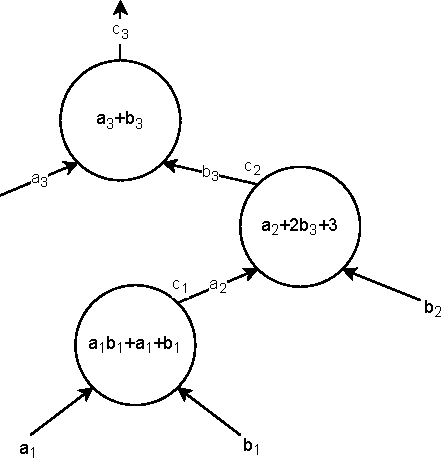
\includegraphics[width=0.4\textwidth]{../figures/plonk-circuit.drawio}
    \caption{Example of a \plonk-like circuit.}
    \label{figure:plonk-circuit-example}
\end{figure}

Observe all the values below depend only on the shape of the circuit itself, so if the circuit does not change, this polynomial should not be recomputed. Check that the \SA, \SB and \SC polynomials are constructed so that we can verify the copy-constraints $c_2 = b_3$ and $c_1 = a_2$ present in the circuit. Observe that equally painted cells have their values swapped, as explained before in the construction of the connection $S$ polynomials.  

\begin{figure}[H]
    \centering
    \begin{tabular}{|c|c|c|c|c|c|c|c|}
        \hline
        \QL	&\QR	&\QM	&\QO	&\QC	&\SA					&\SB						&\SC 							\\ \hline
        1			&1				&1				&-1				&0				&1								&$k_1$								&\cellcolor{pink} $g$				\\
        1			&2				&0				&-1				&3				&\cellcolor{pink}$k_2$			&$k_1 \cdot g$					&\cellcolor{cyan} $k_1 \cdot g^2$	\\
        1			&1				&0				&-1				&0				&$g^2$						&\cellcolor{cyan}$k_2 \cdot g$ &$k_2 \cdot g^2$					\\
        \hline
    \end{tabular}
    \label{table:plonk-circuit-example}
\end{figure}

Therefore, we can derive a PIL program that validates the previous circuit as shown below:
\begin{pil}
    include "config.pil";
    
    namespace Plonk(%N);
    pol constant QL, QR, QM, QO, QC;
    pol constant SA, SB, SC;
    pol constant L1;
    
    pol commit a, b, c;
    
    public pi = a(0);
    
    // Public values check 
    L1 * (a - :pi) = 0;
    
    // Plonk equation 
    pol ab = a*b;
    QL*a + QR*b + QM*ab + QO*c + QC = 0;
    
    // Copy-constraints check 
    {a, b, c} connect {SA, SB, SC};
\end{pil}




%%%%%%%%%%%%%%%%%%%%%%%%%%%%%%%%%%%%%%%%%%%%%%%%%%%%%%%%%%%%%%%%
\subsection{Filling Polynomials}

Until now we have only shown how to specify some kinds of constraints that several polynomials of a certain program described in PIL should satisfy to become \textit{correct}. All these constraints, together with the constant polynomials inherent to the computation itself, specify the transition function underlying the program definition. In other words, changing either any of the constraints or the description of the constant polynomials produces a change in the program we are working on. 

%TODO Check this paragraph
In this section, we are going to use Javascript and \pilcom to generate a specific execution trace for a given PIL. To do so, we are going to compute a valid execution trace for the example of Section \ref{sec:connecting-sm}. As a remark, we will also use the library \texttt{pil-stark} whose utility is to provide a framework to setup, generate and verify proofs, to use a \texttt{FGL} class which mimics a finite field and it is required by some functions that provide the \pilcom package. 

First of all, under the scope of an asynchronous function called \texttt{execute}, we parse the provided PIL (which is, in our case, \texttt{main.pil}) into a Javascript object using the \texttt{compile} function of \pilcom. In code we obtain:
\begin{js}
    const { FGL } = require("pil-stark");
    const { compile } = require("pilcom");
    const path = require("path");
    
    async function execute() {
        const pil = await compile(FGL, path.join(__dirname, "main.pil"));
    }
\end{js}

The \pilcom package also provides two functions that use the \texttt{pil} object to create two crucial objects from it for the construction of the execution trace: the constant polynomials object and the committed polynomials object (using \texttt{newConstPolsArray} and \texttt{newCommitPolsArray} functions, respectively).
\begin{js}
    const { newConstantPolsArray, newCommitPolsArray, compile } = require("pilcom");
    
    async function execute() {
        
        // ... Previous Code
        
        const constPols =  newConstantPolsArray(pil);
        const cmPols = newCommitPolsArray(pil);
    }
\end{js}

Both such objects contain useful information about the PIL itself, such as the provided length of the program $N$, the total number of constant polynomials and the total number of committed polynomials. However, accessing these objects will allow us to fill the entire execution trace for that PIL. We can access a specific position of the execution trace using the syntax:
\begin{js}
    pols.Namespace.Polynomial[i] 
\end{js}
being \texttt{pols} one of the previously introduced \texttt{constPols} and \texttt{cmPols} objects, \texttt{Namespace} being a specific namespace among the ones defined by the PIL files, \texttt{Polynomial} one of the polynomials defined under the scope of the previous namespace and $i$ an integer in the set $[0,N-1]$ representing the row of the current polynomial. Using this we can now start to fill our polynomials. 

In our example, we will use, as inputs for the trace, which are the ones introduced in the \texttt{Main.a} polynomial, an ascending chain of integers from $0$ to $15$ cyclically (because recall that we are only allowed to use $4$ bits integers). We propose here two functions that fill the constant and committed polynomials accordingly. 
\begin{figure}[H]
    \begin{js}
        async function buildConstantPolynomials(constPols, polDeg) {
            
            for (let i=0; i < polDeg; i++) {
                constPols.Global.BITS4[i] = BigInt(i & 0b1111);
                constPols.Global.L1[i] = i === 0 ? 1n : 0n;
                constPols.Negation.RESET[i] = (i % 4) == 3 ? 1n : 0n;
                constPols.Negation.FACTOR[i] = BigInt(1 << (i % 4));
                constPols.Negation.ISLAST[i] = i === polDeg-1 ? 1n : 0n;
            }
        }
    \end{js}
    \caption{Generation of the constant polynomials.}
\end{figure}

\begin{figure}[H]
    \begin{js}
        async function buildcommittedPolynomials(cmPols, polDeg) {
            
            cmPols.Negation.a[-1] = 0n;
            cmPols.Negation.neg_a[-1] = 1n;
            
            for (let i=0; i < polDeg; i++) {
                
                let fourBitsInt = i % 16;
                
                cmPols.Main.a[i] = BigInt(fourBitsInt);
                cmPols.Main.neg_a[i] = BigInt(fourBitsInt ^ 0b1111);
                cmPols.Main.op[i] = FGL.mul(cmPols.Main.a[i], cmPols.Main.neg_a[i]);
                
                cmPols.Multiplier.freeIn1[i] = cmPols.Main.a[i];
                cmPols.Multiplier.freeIn2[i] = cmPols.Main.neg_a[i];
                cmPols.Multiplier.out[i] = cmPols.Main.op[i];
                
                let associatedInt = Math.floor(i/4);
                let bit = (associatedInt >> (i%4) & 1) % 16;
                cmPols.Negation.bits[i] = BigInt(bit);
                cmPols.Negation.nbits[i] = BigInt(bit ^ 1);
                
                
                let factor = BigInt(1 << (i % 4));
                let reset = (i % 4) == 0 ? 1n : 0n;
                cmPols.Negation.a[i] = factor*cmPols.Negation.bits[i] 
                + (1n-reset)*cmPols.Negation.a[i-1];
                cmPols.Negation.neg_a[i] = factor*cmPols.Negation.nbits[i] 
                + (1n-reset)*cmPols.Negation.neg_a[i-1];
            }
        }
    \end{js}
    \caption{Generation of the committed polynomials.}
\end{figure}

Now that we have all the constant and committed polynomials filled in, we can check using a function called \texttt{verifyPil} that they indeed satisfy the constraints defined in the PIL file. We provide below the piece of code that construct the polynomials and check the constraints. If the verification procedure fails, we should not proceed to the proof generation because it will lead to false proof. 
\begin{js}
    const { newConstantPolsArray, newCommitPolsArray, compile, verifyPil } = require("pilcom");
    
    async function execute() {
        
        // ... Previous Code	
        
        const N = constPols.Global.BITS4.length;
        
        await buildConstantPolynomials(constPols, N);
        await buildcommittedPolynomials(cmPols, N);
        
        const res =  await verifyPil(FGL, pil, cmPols , constPols);
        if (res.length != 0) {
            console.log("The execution trace do not satisfy PIL restrictions. Aborting...");
            for (let i=0; i<res.length; i++) {
                console.log(res[i]);
                return;
            }
        }
    }
\end{js}







%TODO: Is this section necessary?
%%%%%%%%%%%%%%%%%%%%%%%%%%%%%%%%%%%%%%%%%%%%%%%%%%%%%%%%%%%%%%%%%
\subsection{Generating a Proof Using \texttt{pil-stark}}

Once the constant and the committed polynomials are filled, we can step to the proof generation stage. We can use the \texttt{pil-stark} Javascript package specially designed to work together with \pilcom to generate STARK proofs about PIL statements. We will use three functions \texttt{starkSetup}, \texttt{starkGen} and \texttt{starkVerify} from the package. The first one is aiming for setting up the STARK, which is independent of the values of committed polynomials. This includes the computation of the tree of the evaluations of the constant polynomials. For executing the setup generation we ought to have an object called \texttt{starkStruct} which is specifying several FRI-related parameters such as the size of the trace domain (which must coincide with $N$, defined in PIL), the size of the extended domain (which together with the previous parameter specifies the correspondent \textit{blowup factor}), the number of queries to be executed and the reduction factors for each of the FRI steps. We execute the setup using the code below:

\begin{js}
    const { FGL, starkSetup } = require("pil-stark");
    
    async function execute() {
        
        // ... Previous Code	
        
        const starkStruct = {
            "nBits": 10,
            "nBitsExt": 11,
            "nQueries": 128,
            "verificationHashType": "GL",
            "steps": [
            {"nBits": 11},
            {"nBits": 5},
            {"nBits": 3},
            {"nBits": 1}
            ]
        };
        
        const setup = await starkSetup(constPols, pil, starkStruct);
    }
\end{js}

Now that we have set up the STARK, we can generate the proof using the \texttt{starkGen} function. We can do this task using the code below. Observe that the \texttt{setup} object contains inside a \texttt{starkInfo} field which contains, aside from all the \texttt{starkStruct} parameters, lots of useful information about the shape of the PIL itself. 

\begin{js}
    const { FGL, starkSetup, starkGen } = require("pil-stark");
    
    async function execute() {
        
        // ... Previous Code	
        
        const resProof = await starkGen(cmPols, constPols, setup.constTree, setup.starkInfo);
    }
\end{js}

Now that a proof has been generated we can be involved in the verification procedure invoking the \texttt{starkVerify} function. This function needs, as arguments, some information provided by the outputs of both the \texttt{starkSetup} and \texttt{starkGen} functions. If the output of the \texttt{starkVerify} function is \texttt{true}, the proof is valid. Otherwise, the verifier should invalidate the proof sent by the prover. 

\begin{js}
    const { FGL, starkSetup, starkGen, starkVerify } = require("pil-stark");
    
    async function execute() {
        
        // ... Previous Code
        
        const resVerify = await starkVerify(
        resP.proof, resP.publics, setup.constRoot, setup.starkInfo
        );
        
        if (resVerify === true) {
            console.log("The proof is VALID!");
        } else {
            console.log("INVALID proof!");
        }
    }
\end{js}


%%%%%%%%%%%%%%%%%%%%%%%%%%%%%%%%%%%%%%%%%%%%%%%%%%%%%%%%%%%%%%% 
\section{zkASM instructions set} \label{sec:instructions}

\subsection{Memory Related Instructions}


We refer to the memory as a volatile read-write data storage that exists only during the execution of a zkASM program. The memory is divided into different contexts of \texttt{0x40000} words. Each word is 256 bits in length, so each context is 8 MB in size.

Each context is divided into the following three blocks:

\begin{itemize}
    
    \item \textbf{VARS:} With a relative offset of \texttt{0x00000} and a height of \texttt{0x10000} words (\texttt{2MB}), contains the local context variables pre-defined in the language. The list of all context variables can be found at \href[]{https://github.com/0xPolygonHermez/zkevm-rom/blob/main/main/vars.zkasm}{\texttt{vars.zkasm}}.
    
    \item \textbf{STACK:} With a relative offset of \texttt{0x10000} and a height of \texttt{0x10000}  words  \texttt{(2MB)}, contains the stack of the the EVM. \textbf{STACK} is defined once per context.
    
    \item \textbf{MEMORY:} With a relative offset of \texttt{0x20000} and a height of \texttt{0x20000} words \texttt{(4MB)}, contains the free memory that can be freely used. \textbf{MEMORY}, like \textbf{STACK}, is also defined once per context. 
\end{itemize}

Therefore, for a given slot in memory, its pointer is computed as:
\[
\texttt{memoryAddress} = \texttt{0x40000} \cdot \texttt{CTX} + \texttt{isStack} \cdot (\texttt{0x10000} + \texttt{SP}) + \texttt{isMem} \cdot (\texttt{0x20000} + \texttt{offset})
\]
where:

\begin{itemize}
    
    \item \texttt{CTX}: This integer variable refers to the memory context being accessed in the EVM's memory. 
    
    \item \texttt{isStack}:  this boolean value indicates whether the memory operation being performed is related to the EVM's stack. The EVM uses a stack-based architecture, meaning that operations are performed by pushing and popping values on and off the stack.
    
    \item \texttt{SP}: This variable refers to the current position of the stack pointer in the EVM's stack. The stack pointer is used to keep track of the current top of the stack. More information on \texttt{SP} will be added below.
    
    \item \texttt{isMem}: This boolean value indicates whether the memory operation being performed is related to the EVM's memory. Observe that \texttt{isStack} and \texttt{isMem} can not be $1$ at the same time. 
    
    \item \texttt{offset}:  This variable likely refers to the offset or location within the current memory context being accessed.
    
\end{itemize}

Observe that, following the above description of the memory, the former set of variables completely determine a memory slot. Figure ?? shows the structure of the memory during a zkASM execution.

\begin{figure}[H]
    \centering
    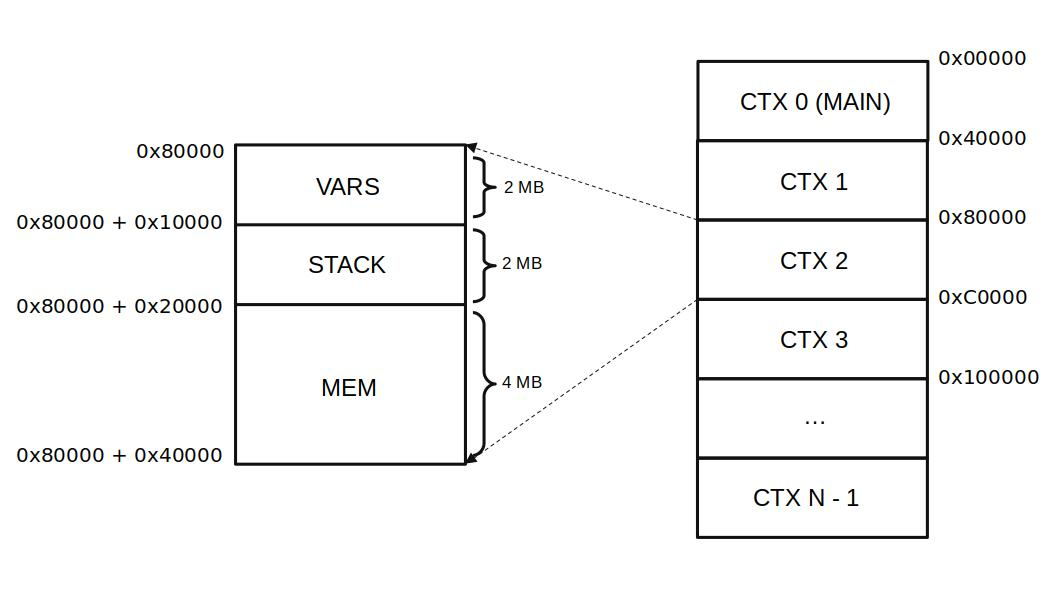
\includegraphics[width=0.6\columnwidth]{\assemblydir/figures/memory-regions}
    \caption{Schema of contexts and memory regions of the zkEVM.}
    \label{fig:memory-regions}
\end{figure}

In order to allow runtime interaction with memory, zkASM has a couple of instructions to read and write values to it.



Let us first define how can be access to a specific address of the memory. Memory acess will be parametrized by $2$ integer parameters: the address \addr and the relative address \relAddr. 

\begin{itemize}

\item \addr: Address would be able to define a memory access up to memory region level. That is, \addr will contain information of which context access the memory and if the access is directed to the system variables \textbf{VARS}, the \textbf{STACK} or the \textbf{MEMORY}.

\item \relAddr: However, \addr is not enough. Hence, \relAddr will point to a specific memory slot inside a concrete memory region of a context. We should take into account that \relAddr can never be negative. Moreover, \relAddr is also bounded from above: if we are accessing to the \textbf{MEMORY}, \relAddr should be strictly less than \texttt{0x40000} (because memory measures $\texttt{4MB}$) and if we are accessing to the \textbf{STACK} or to the system variables \textbf{VARS}, \relAddr should be strictly less than \texttt{0x10000} (because both memory regions measure $\texttt{2MB}$). Then, the wanted memory slot will be equal to $\addr + \relAddr$.

\end{itemize}

Let us know how to specify \addr and \relAddr in zkASM language. We can specify \addr with $3$ keywords: \texttt{SYS} (which corresponds to \textbf{VARS} memory region), \texttt{STACK} (which corresponds to \textbf{STACK} memory region) and \texttt{MEM} (which corresponds to \textbf{MEMORY} memory region). Invoking \texttt{STACK} will increase \addr by $\texttt{0x10000}$ and similarly, invoking \texttt{MEM} will increase \addr by \texttt{0x20000}. However, since \textbf{VARS} is the first memory region, it will not produce an increase in \addr. Moreover, \addr will also increase depending on the current context. More specifically, a total amount of \texttt{0x40000} will be increased per context, following our memory description above. 

To specify \relAddr we can use $2$ registers: \E and \RR. If \E is chosen, \relAddr will increase a total amount of $\E_0$ units. Similarly, if \RR is chosen, \relAddr will increase by \RR. Moreover, we can add a numeric offset to increase a fixed amount of units \addr + \relAddr. 

The syntax will be, in each case:

\begin{zkasm}
addr:relAddr 
; or
addr:relAddr+offset
; or 
addr:relAddr-offset
\end{zkasm}

Below, we specify concrete examples on how to specify addresses:

\begin{zkasm}
SYS:E
SYS:E+1
STACK:RR
MEM:E 
MEM:E-2
MEM:RR+1
\end{zkasm}

To end up, we can also access to addresses by means of global and local variables, defined elsewhere in the assembly code. This variables will have a unique identifier that we will use in order to access to it.


\subsubsection{\MLOAD}


\MLOAD is the zkASM instruction used to read a value from a specific address in memory. It takes the pointer address of the memory slot to be read as a parameter. We can store the value that is read in a register of our choosing by using the free input (\texttt{\$}) assignment. 

Suppose that we want to read the memory value stored in the address \texttt{someAddr} in a certain context. The address \texttt{someAddr} is defined by the global variable:
\begin{zkasm}
VAR GLOBAL someAddr
\end{zkasm}

The following zkASM code stores the corresponding value into the register \A:
\begin{zkasm}
$ => A          :MLOAD(someAddr)
\end{zkasm}





\subsubsection{\MSTORE}


\MSTORE is the zkASM instruction used to write a value to a specific address in memory. It takes the pointer address of the memory slot to be read as a parameter, the register that contains the value to be writed must be also specified.

The following example shows how to store in the memory the value of the current context. Note that as the \MSTORE parameter, it is specified the variable that contains the pointer to where current context is stored in the memory. The value stored will be taken from \texttt{CTX} register:
\begin{zkasm}
CTX       :MSTORE(currentCTX)      
\end{zkasm}



\subsubsection{Dealing with the STACK}

A stack machine is a machine in which temporary values for computations are moved to and from a push down stack. Operations over the stack are the typical: \texttt{PUSH}, \texttt{POP}, \texttt{DUP}, \texttt{SWAP}, etc. Since the EVM is a stack-based virtual machine, we reserve an address space to create a stack within the memory of the zkEVM. The classical pointer called \texttt{STACK POINTER} (\texttt{SP}) contains the address of the \textbf{next free position on the} \texttt{STACK}. A \texttt{POP} from the \texttt{STACK} can be implemented as:

\begin{zkasm}
SP -1 => SP
$ => A		:MLOAD(SP)
\end{zkasm}

where we decrement \texttt{SP} to reposition it on the last element of the stack and
then we load this element into registry \A. Similarly, a \texttt{PUSH} into the \texttt{STACK} can be implemented as:

\begin{zkasm}
0		:MSTORE (SP++)
\end{zkasm}

which saves a \texttt{0} at the top of the stack and increments \texttt{SP}. An important note about both the stack and the memory is that the stack pointer and the memory are per context.




\subsubsection{\MEMALIGNRD}

Although the memory word in zkASM is 256 bits long, in roder to mimic the regular Ethereum Virtual Machine (EVM) memory behavior, zkASM has a specific instructions for accessing memory at the byte level. The instruction \MEMALIGNRD enables reading 32 bytes starting from an offset of any byte in memory. In this way, two memory registers are read and a the following transformation is applied to virtually obtain a new 32-byte word as a result of the reading.
\begin{align*}
    \texttt{val} &= \Bigr[ \texttt{m}_0 \ll 8 \cdot \texttt{offset} \Bigr] \mathbin\Vert \Bigr[ \texttt{m}_1 \gg 256- 8 \cdot \texttt{offset} \Bigr] 
\end{align*}

Here, the symbol $\mathbin\Vert$ denotes string concatenation. The registers must be set as follows before call the \MEMALIGNRD instruction. We can store the value that is read in a register of our choosing by using the free input (\texttt{\$}) assignment.


\begin{figure}[h!]
    \renewcommand{\figurename}{Table}
    \[
    \begin{array}{|c|c|}
        \hline
        \mathbf{Register} &\mathtt{MEM\_ALIGN\_RD} \ \mathbf{parameters} \\ \hline
        \A & \texttt{Memory Slot of } \mathtt{m_0} \\
        \B & \texttt{Memory Slot of } \mathtt{m_1} \\
        \C & \texttt{offset} \\
        \hline
    \end{array}
    \]
    \caption{\MEMALIGNRD instruction parameters.}
    \label{tab:memory-first-example}
\end{figure}

The following example shows how to read 32 bytes that are stored occupying part of two consecutive zkASM memory words. The read value will be stored in register \A:

\begin{zkasm}
$ => A          :MLOAD(someAddr)
$ => B          :MLOAD(someAddr+1)
16 => C

$ => A          :MEM_ALIGN_RD
\end{zkasm}

Figure ?? shows how the 32-bytes value will be read for the \MEMALIGNRD given example.

\begin{figure}[H]
    \centering
    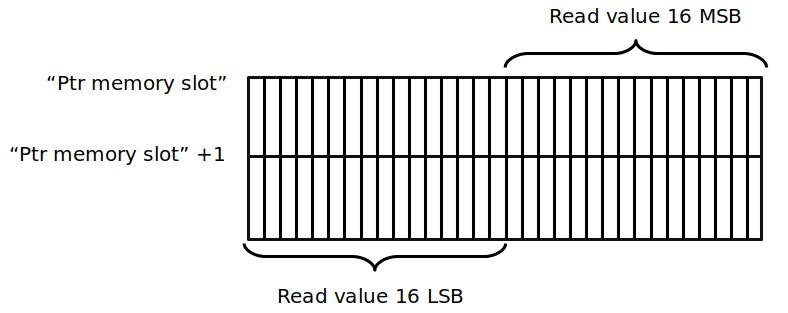
\includegraphics[width=0.8\columnwidth]{\assemblydir/figures/mem-align-wr}
    \caption{Example of how values are read from the memmory using \MEMALIGNRD with an offset of 16.}
    \label{fig:memory-regions}
\end{figure}

\subsubsection{\MEMALIGNWR}
\MEMALIGNWR is equivalent to \MEMALIGNRD but for writing a 32-byte value. In this case, we have to specify two memory slots that will be written after applying the following transformation to the value to be stored. The registers that contains the value to be stored must also be specified.
\begin{align*}
    \texttt{w}_0 &= \Bigr[ \texttt{m}_0 \ \texttt{\&} \ \left(2^{256} - 2^{256-8 \cdot \texttt{offset}} \right) \Bigr] \mathbin\Vert \Bigr[  \texttt{val} \ll 8 \cdot \texttt{offset} \Bigr]  \\
    \texttt{w}_1 &= \Bigr[ \texttt{m}_1 \ \texttt{\&} \ \left( \left( 2^{256} - 1\right)  \gg 8 \cdot \texttt{offset}\right) \Bigr] \mathbin\Vert \Bigr[ \texttt{val} \ll 8 \cdot \texttt{offset} \Bigr] 
\end{align*}

\begin{figure}[h!]
    \renewcommand{\figurename}{Table}
    \[
    \begin{array}{|c|c|}
        \hline
        \mathbf{Register} &\mathtt{MEM\_ALIGN\_WR} \ \mathbf{parameters} \\ \hline
        \A & \texttt{Memory Slot of } \mathtt{m_0}  \\
        \B & \texttt{Memory Slot of } \mathtt{m_1}  \\
        \C & \mathtt{offset} \\
        \D & \mathtt{w_0} \\
        \E & \mathtt{w_1} \\
        \op& \texttt{Value to be written} \\
        \hline
    \end{array}
    \]
    \caption{\MEMALIGNWR instruction parameters.}
    \label{tab:memory-first-example}
\end{figure}

The following example shows how to write 32 bytes that are stored occupying part of two consecutive zkASM memory words. The value to be stored will be taken from free input register:

\begin{zkasm}
$ => A          :MLOAD(MEM:E)
$ => B          :MLOAD(MEM:E+1)

${memAlignWR_W0(A,mem.bytesToStore,C)} => D                    ; no trust calculate W0
${memAlignWR_W1(B,mem.bytesToStore,C)} => E                    ; no trust calculate W1
$               :MEM_ALIGN_WR,MLOAD(bytesToStore)
\end{zkasm}

\subsubsection{\MEMALIGNWRE}

\MEMALIGNWRE allows writing only 8 bits of a specific memory slot. In this case, we have to specify the memory slot to be written, the register that contains the byte to be stored, and the offset value that situates the byte in a specific position of the 32-byte word. The value will be written after applying the following transformation:
\begin{align*}
    \texttt{w}_0 &= \Bigr[ \texttt{m}_0 \ \texttt{\&} \ \left( \texttt{maskByte} \gg 8 \cdot \texttt{offset} \right) \Bigr]  \mathbin\Vert \Bigr[ \left( \texttt{bits} \ \texttt{\&} \ \texttt{0xFF} \right)  \ll 8 \cdot \left( 31-\texttt{offset}\right) \Bigr] 
\end{align*}
where $\texttt{maskByte}$ equals $2^{256} - 1$. 

\begin{figure}[h!]
    \renewcommand{\figurename}{Table}
    \[
    \begin{array}{|c|c|}
        \hline
        \mathbf{Register} &\mathtt{MEM\_ALIGN\_WR8} \ \textbf{parameters} \\ \hline
        \A & \texttt{Memory Slot of } \mathtt{m_0} \\
        \C & \mathtt{offset} \\
        \D & \mathtt{w_0} \\
        \op& \texttt{Value to be written} \\
        \hline
    \end{array}
    \]
    \caption{\MEMALIGNWRE instruction parameters.}
    \label{tab:memory-first-example}
\end{figure}

The following example shows how to write $1$ bytes stored in the byte $4$ of a specific storage slot. The value to be stored will be taken from \B register:

\begin{zkasm}
4 => C
$ => A          :MLOAD(someAddr)
${memAlignWR8_W0(A,B,C)} => D  ; no trust calculate W0
B               :MEM_ALIGN_WR8 ; only use LSB of B, rest of bytes could be non zero
\end{zkasm}

\subsection{Storage Related Instructions}

Polygon zkEVM, like Ethereum L1, has a storage component for storing persistent on-chain data, which includes the balances of all accounts, their nonces, and the state of all deployed smart contracts along with their codes. The data that forms the state is represented as cryptographic trie, but while Ethereum L1 uses a modified Patricia tree with Keccak256 as the hash operation, Polygon zkEVM uses a binary sparse Merkle tree with Poseidon as the hash operation (refer to the technical documents regarding the zkEVM bridge annex A to learn more about sparse Merkle trees).

Poseidon is a hash function that's specifically designed for use in zero-knowledge applications, as it's meant to operate with values of a prime field and it has been proven to be much more performant than Keccak256 in zero-knowledge constructions like those used in Polygon zkEVM. Moreover Poseidon hash has an input named capacity, which can be used as an extra input value.

Barely, the Polygon zkEVM state tree is a key-value structure in which the integrity can be ensured by a 256-bit value known as the state root. Each entry in the tree is a leaf and directly stores a 256-bit value. Additionally, the index position of that leaf in the tree corresponds to the 256-bits of the key. As can be seen in Figure X, since the keys are 256-bits in length, the tree has 32 levels and a total capacity of $2^{256}$ leaves.


\begin{figure}[H]
    \centering
    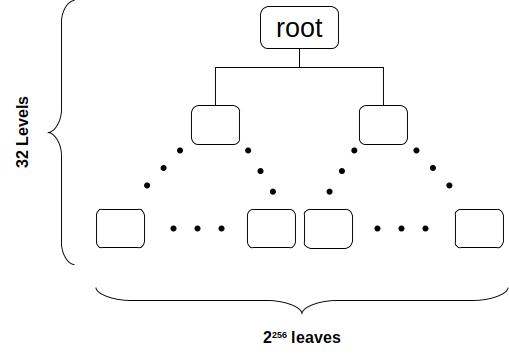
\includegraphics[width=0.6\columnwidth]{\assemblydir/figures/state-trie}
    \caption{Polygon zkEVM state trie.}
    \label{fig:hashk-add-bytes}
\end{figure}

Since five different types of values can be stored, a distinction must be made among the five types of leaves. Table X shows the relation between leaf type and the corresponding data types that they contain.

\begin{figure}[h!]
    \renewcommand{\figurename}{Table}
    \[
    \begin{array}{|c|c|}
        \hline
        \mathbf{Leaf~type} &\mathbf{Data~type} \\ \hline
        \mathtt{0} & \mathtt{Account~balance} \\
        \mathtt{1} & \mathtt{Account~nonce} \\
        \mathtt{2} & \mathtt{Contract~code~hash} \\
        \mathtt{3} & \mathtt{Contract~storage~slot~value} \\
        \mathtt{4} & \mathtt{Contract~code~length} \\
        \hline
    \end{array}
    \]
    \caption{Polygon zkEVM state tree leaf types.}
    \label{tab:memory-first-example}
\end{figure}


For each leaf entered in the tree its key is computed as follows:

$$\texttt{key} = \texttt{Poseidon}(\texttt{key\_seed})$$

where \texttt{key\_seed} is a $32$-bytes integer constructed as follows:
\[
\texttt{key\_seed} = (\texttt{account\_address} \mid\mid \texttt{0x00000000} \mid\mid \texttt{leaf\_type} \mid\mid \texttt{0x00000000})
\]
being $\texttt{account\_address} \in \{0, 1, \dots, 2^{160} - 1\}$ is a $20$-bytes integer and $\texttt{leaf\_type} \in \{0, 1, \dots, 2^{32} - 1\}$ a $4$-bytes integer.

The capacity of the Poseidon's instance used when computing keys is always zero except in the case where the leaf corresponds to a contract storage slot value (leaf type 3), in which case the capacity is directly set to the storage slot pointer. It's important to note that because the contract storage slot pointer is not encoded in the 32-byte input, if we do not use the capacity, all storage slots for the same contract would lead to the same state tree leaf.

Te value sored in the leaf has the following structure:
\[
(v_0, \dots, v_7)
\]
codifying a $256$-bits unsigned integer, where $v_i \in \FF_p$ are bounded to $32$-bits each. 

In order to allow runtime interaction with the Polygon zkEVM state tree zkASM has a couple of instructions to read and write values on it.

\subsubsection{\texttt{SLOAD}}

\texttt{SLOAD} is the zkASM instruction used to read a value from a leaf in the state tree. It takes Poseidon's ``Input" and ``Capacity" parameters, along with the leaf type, to compute the key of the leaf to be read. The registers must be set as follows before call the \texttt{SLOAD} instruction.

\begin{figure}[h!]
    \renewcommand{\figurename}{Table}
    \[
    \begin{array}{|c|c|}
        \hline
        \mathbf{Register} &\texttt{SLOAD } \textbf{parameters} \\ \hline
        \A & \mathtt{Account~address} \\
        \B & \mathtt{Leaf~type} \\
        \C & \mathtt{Contract~storage~slot~pointer~(capacity)} \\
        \hline
    \end{array}
    \]
    \caption{\texttt{SLOAD} instruction parameters.}
    \label{tab:memory-first-example}
\end{figure}

We can store the value that is read in a register of our choosing by using the free input (\texttt{\$}) assignment.

The following example shows how to read the balance of a specific account, the value that is read will be stored in the \E register:

\begin{zkasm}
someAccountAddr => A          
0 => B      
0 => C          
$ => E          :SLOAD
\end{zkasm}

The following example shows how to read a storage slot of a specific contract, the value that is read will be stored in the \E register:

\begin{zkasm}
someAccountAddr => A          
3 => B      
storageSlotPtr => C 
$ => E          :SLOAD
\end{zkasm}

\subsubsection{\texttt{SSTORE}}

\texttt{SSTORE} is the zkASM instruction used to store a value to a leaf in the state tree. It takes Poseidon's ``Input" and ``Capacity" parameters, along with the leaf type, to compute the key of the leaf to be writen, in addition takes the value to be written. The registers must be set as follows before call the \texttt{SSTORE} instruction.

\begin{figure}[h!]
    \renewcommand{\figurename}{Table}
    \[
    \begin{array}{|c|c|}
        \hline
        \mathbf{Register} &\texttt{SSTORE } \textbf{parameters} \\ \hline
        \A & \mathtt{Account~address} \\
        \B & \mathtt{Leaf~type} \\
        \C & \mathtt{Contract~storage~slot~pointer~(capacity)} \\
        \D & \mathtt{Value~to~write} \\
        \hline
    \end{array}
    \]
    \caption{\texttt{SSTORE} instruction parameters.}
    \label{tab:memory-first-example}
\end{figure}

The following example shows how to write a storage slot of a specific contract:

\begin{zkasm}
someAccountAddr => A          
3 => B      
storageSlotPtr => C          
value => D         
A               :SSTORE
\end{zkasm}




%%%%%%%%%%%%%%%%%%%%%%%%%%%%%%%%%%%%%%%%%%%%%%%%%%%%%%%%%%%%%%%

\subsection{Binary-Related Instructions}

The arithmetic operators are used to perform arithmetic mathematical operations on numeric data stored in registers.

\subsubsection{\ADD}

\ADD is used to sum the content of the registers \A and \B, the result will be treated as a free input. The following example shows how to use \ADD instruction.

\begin{zkasm}
val1 => A          
val2 => B          

$ => C             :ADD ; [ val1 + val2 => C]
\end{zkasm}

\subsubsection{\SUB}

\SUB is used to subtract de content fo register \B to \A, the result will be treated as a free input. The following example shows how to use \SUB instruction.

\begin{zkasm}
val1 => A          
val2 => B          

$ => C             :SUB ; [ val1 - val2 => C]
\end{zkasm}



\subsubsection{\LT}

\LT instruction is used to compare the values of the registers \A and \B as \textbf{unsigned integers}. The output of the operation will be $1$ if \A is actually lower than \B (that is, $\A < \B$) and $0$ otherwise (that is, $\A \geq \B$). The output of the instruction will be treated as a free input. The next lines of code show an example on how to use \LT instruction:

\begin{zkasm}
valA => A
valB => B

$ => C			:LT ; [1 if A < B, 0 if A <= B]
\end{zkasm}





\subsubsection{\SLT}

\SLT instruction is used to compare the values of the registers \A and \B as \textbf{signed integers}, explained in Section \ref{sec:binary-sm}. The output of the operation will be $1$ if \A is actually lower than \B (that is, $\A < \B$) and $0$ otherwise (that is, $\A \geq \B$). The output of the instruction will be treated as a free input. The next lines of code show an example on how to use \SLT instruction:

\begin{zkasm}
valA => A
valB => B

$ => C			:SLT ; [1 if A < B, 0 if A <= B]
\end{zkasm}


\subsubsection{\EQ}

\EQ instruction is used to compare the equality relationship between the values of the registers \A and \B. The output of the operation will be $1$ if \A is equal to \B (that is, $\A = \B$) and $0$ otherwise (that is, $\A \neq \B$). The output of the instruction will be treated as a free input. The next lines of code show an example on how to use \EQ instruction:

\begin{zkasm}
valA => A
valB => B

$ => C			:EQ ; [1 if A = B, 0 if A != B]
\end{zkasm}


\subsubsection{\AND}


\AND instruction is used to perform the bit-wise \AND operation between registers \A and \B, as explained in Section \ref{sec:binary-sm}. The output of the instruction will be treated as a free input. The next lines of code show an example on how to use \AND instruction:

\begin{zkasm}
valA => A
valB => B

$ => C			:AND
\end{zkasm}

For sake of completeness, let us propose a more concrete example, where we assign the value $\texttt{0xDBn}$ to \A and the value $\texttt{0x86n}$ to \B. The result of the bit-wise \AND operation is going to be \texttt{0x82n} because
\[
\A = \texttt{0b11011011}, \quad \B = \texttt{0b10000110} \Longrightarrow \C = \texttt{0b10000010}.
\]

\begin{zkasm}
0xDBn => A
0x86n => B

$ => C			:AND ; C = 0x82n
\end{zkasm}

\subsubsection{\OR}

\OR instruction is used to perform the bit-wise \OR operation between registers \A and \B, as explained in Section \ref{sec:binary-sm}. The output of the instruction will be treated as a free input. The next lines of code show an example on how to use \OR instruction:

\begin{zkasm}
valA => A
valB => B

$ => C			:OR
\end{zkasm}

For sake of completeness, let us propose a more concrete example, where we assign the value $\texttt{0xDBn}$ to \A and the value $\texttt{0x86n}$ to \B. The result of the bit-wise \OR operation is going to be \texttt{0xDFn} because
\[
\A = \texttt{0b11011011}, \quad \B = \texttt{0b10000110} \Longrightarrow \C = \texttt{0b11011111}.
\]

\begin{zkasm}
0xDBn => A
0x86n => B

$ => C			:OR ; C = 0xDFn
\end{zkasm}



\subsubsection{\XOR}

\XOR instruction is used to perform the bit-wise \XOR operation between registers \A and \B, as explained in Section \ref{sec:binary-sm}. The output of the instruction will be treated as a free input. The next lines of code show an example on how to use \XOR instruction:

\begin{zkasm}
valA => A
valB => B

$ => C			:XOR
\end{zkasm}

For sake of completeness, let us propose a more concrete example, where we assign the value $\texttt{0xDBn}$ to \A and the value $\texttt{0x86n}$ to \B. The result of the bit-wise \XOR operation is going to be \texttt{0x5Dn} because
\[
\A = \texttt{0b11011011}, \quad \B = \texttt{0b10000110} \Longrightarrow \C = \texttt{0b01011101}.
\]

\begin{zkasm}
0xDBn => A
0x86n => B

$ => C			:XOR ; C = 0x5Dn
\end{zkasm}





%%%%%%%%%%%%%%%%%%%%%%%%%%%%%%%%%%%%%%%%%%%%%%%%%%%%%%%%%%%%%%%
\subsection{Arithmetic-Related Instructions}

\subsubsection{\ARITH}

The \ARITH instruction allows to check field operations. More specifically, it checks a combination of an addition and a product, as explained in Section \ref{sec:arith-sm}. Before calling the \ARITH instruction, registers \A, \B, and \C must be set. The equation that follows will be evaluated using the values of these $3$ registers. It is necessary to specify where the result of the evaluation will be stored. If the evaluation results in an overflow of the output register, the overflow value will be stored in register \D. More specifically, the equation that checks the \ARITH instruction is the following one:

\[
\D \cdot 2^{256} + \op = \A \cdot \B + \C
\]

The following example shows how to use \ARITH instruction. The result of the evaluation will be stored in register \A, and if there is an overflow, it will be stored in register \D:
\begin{zkasm}
valA => A          
valB => B          
valC => C
A            :ARITH ; [ valA * valB + valC => [D,A]]
\end{zkasm}





\subsubsection{\ARITHADDDIFF}

The \ARITHADDDIFF instruction allows to perform additions $P + Q$ over the elliptic curve defined in Section \ref{sec:arith-sm}. This instruction can not perform doublings, since the input points to be added are supposed to be different. This is not explicitly check, but since the doubling formula differs a lot from the distinct point addition formula, the result will be wrong if $P = Q$. The input parameters of the instruction are specified in the table below:

\begin{figure}[h!]
    \renewcommand{\figurename}{Table}
    \[
    \begin{array}{|c|c|}
        \hline
        \mathbf{Register} &\texttt{ARITH\_ECADD\_DIFFERENT } \textbf{parameters} \\ \hline
        \A & x_1, \mathtt{~x~coordinate~of~}P \\
        \B & y_1, \mathtt{~y~coordinate~of~}P \\
        \C & x_2, \mathtt{~x~coordinate~of~}Q \\
        \D & y_2, \mathtt{~y~coordinate~of~}Q \\
        \E & x_3, \mathtt{~x~coordinate~of~}P+Q \\
        \op & y_3, \mathtt{~y~coordinate~of~}P+Q \\
        \hline
    \end{array}
    \]
    \caption{\ARITHADDDIFF instruction parameters.}
    \label{tab:memory-first-example}
\end{figure}

An example on how to use the \ARITHADDDIFF instruction can be seen in the code blow. Observe that we make use of the executor implemented functions \texttt{xAddPointEc(A,B,C,D)} and \texttt{yAddPointEc(A,B,C,D)} which compute the $x$ and the $y$ coordinate of $P + Q$ being $P = (A, B)$ and $Q = (C, D)$ whenever $P \neq Q$. After this is computed, the $x$ coordinate of $P + Q$ is is stored into the memory slot given by the address \texttt{addX} and, similarly, the $y$ coordinate of $P + Q$ is pushed into the memory slot given by the address \texttt{addY}. If we have used incorrect values for the coordinates of $P + Q$, an executor error will pop. This will also be captured when the proof of the batch is generated, since the instruction invocation fills the polynomials of the Arithmetic State Machine correctly. 

\begin{zkasm}
$ => A  						:MLOAD(Px)
$ => B  						:MLOAD(Py)
$ => C  						:MLOAD(Qx)
$ => D  						:MLOAD(Qy)
${xAddPointEc(A,B,C,D)} => E  	:MSTORE(addX)
${yAddPointEc(A,B,C,D)} 		:ARITH_ECADD_DIFFERENT, MSTORE(addY)
\end{zkasm}


\subsubsection{\ARITHADDSAME}

The \ARITHADDSAME instruction allows to perform point doublings $2P$ over the elliptic curve defined in Section \ref{sec:arith-sm}. The input parameters of the instruction are specified in the table below:

\begin{figure}[h!]
    \renewcommand{\figurename}{Table}
    \[
    \begin{array}{|c|c|}
        \hline
        \mathbf{Register} &\texttt{ARITH\_ECADD\_DIFFERENT } \textbf{parameters} \\ \hline
        \A & x_1, \mathtt{~x~coordinate~of~}P \\
        \B & y_1, \mathtt{~y~coordinate~of~}P \\
        \E & x_3, \mathtt{~x~coordinate~of~}2P \\
        \op & y_3, \mathtt{~y~coordinate~of~}2P \\
        \hline
    \end{array}
    \]
    \caption{\ARITHADDDIFF instruction parameters.}
    \label{tab:memory-first-example}
\end{figure}

An example on how to use the \ARITHADDSAME instruction can be seen in the code blow. Observe that we make use of the executor implemented functions \texttt{xDblPointEc(A,B)} and \texttt{yDblPointEc(A,B)} which compute the $x$ and the $y$ coordinate of $2P$ being $P = (A, B)$. After this is computed, the $x$ coordinate of $2P$ is is stored into the memory slot given by the address \texttt{doublePx} and, similarly, the $y$ coordinate of $2P$ is pushed into the memory slot given by the address \texttt{doublePy}. If we have used incorrect values for the coordinates of $2P$, an executor error will pop. This will also be captured when the proof of the batch is generated, since the instruction invocation fills the polynomials of the Arithmetic State Machine correctly. 

\begin{zkasm}
$ => A  					:MLOAD(Px)
$ => B  					:MLOAD(Py)

${xDblPointEc(A,B)} => E  	:MSTORE(doublePx)
${yDblPointEc(A,B)} 		:ARITH_ECADD_SAME, MSTORE(doublePy)
\end{zkasm}









%%%%%%%%%%%%%%%%%%%%%%%%%%%%%%%%%%%%%%%%%%%%%%%%%%%%%%%%%%%%%%%
\subsection{Execution Control Flow Related Instructions}

In order to allow to conditional branch execution of the zkASM programs, 4 different instruction has been included in zkASM instructios set.

\subsubsection{\JMP} % Jump
\JMP is an unconditional jump instruction that always causes a jump in the program's execution flow, regardless of any conditions. It takes an address of the ROM as a parameter to continue the execution flow. To avoid using numeric pointers for jumps, zkASM allows jump destinations to be aliased with custom names. The compiler resolves these aliases and substitutes them with pointers later on.

The following code shows the general usage of \JMP instruction:

\begin{zkasm}
    
; ...
; Executed Code
; ...

        :JMP(destinationLabel)

; ... 
; Non Executed Code
; ... 

destinationLabel:

; ...
; Executed Code
; ...
    
\end{zkasm}

Moreover, we can also parametrize the destination of a jump-like instruction using either the first limb of the register $\E_0$ or the register \RR, using the syntax below:

\begin{zkasm}
        :JMP(RR)
        :JMP(E)
\end{zkasm}

For example, the code below will produce a jump of $5$ units in the execution flow:

\begin{zkasm}
5 => E
            :JMP(E)          
\end{zkasm}

The former syntax will be also available for all the other kind of jumps specified in below sections, including the ones having an else clause.

\subsubsection{\JMPN} % Jump if Negative

\JMPN is a conditional jump instruction that causes a jump in the program's execution flow if a specified register contains a negative number. It takes the address of the ROM as a parameter to continue the execution flow. The register that contains the value to be evaluated must also be specified.

In the following example, the execution flow will be redirected to \texttt{stackUnderflow} in the case that the evaluation of $\SP - 2$ leads to a negative number.

\begin{zkasm}
; check stack underflow
SP - 2          :JMPN(stackUnderflow)
\end{zkasm}

Conditional jumps can also receive an else-clause label. The synatx is very similar:

\begin{zkasm}
A					:JMPN(ifClauseLabel, elseClauseLabel)


ifClauseLabel:
        ; do something
        
        
elseClauseLabel:
        ; do something different
\end{zkasm}

If the value stored in the \A register is negative, then the execution of the program will continue under the \texttt{ifClauseLabel} label. However, if the value of \A is bigger or equal than $0$, then the execution will continue from the label \texttt{elseClauseLabel}. 




\subsubsection{\JMPC} % Conditional jump, if a condition is fullfiled

\JMPC is a conditional jump instruction that causes a jump in the program's execution flow if a specified condition is evaluated  as true. It is used along with the following comparative instructions.
\begin{itemize}
    \item \EQ: Evaluates if register \A value is equal to register \B value.
    \item \LT: Evaluates if register \A value is less than register \B value.
    \item \SLT: Evaluates if register \A value is less than register \B value also comparing negative values.
\end{itemize}

In the following example, the execution flow will be redirected to \texttt{absIsNeg} in the case that the value contained in register \A (namely \val) is a negative number.

\begin{zkasm}
val => A
0 => B
$          :SLT, JMPC(absIsNeg)
\end{zkasm}





\subsubsection{\JMPZ} % Jump if Zero

\JMPZ is a conditional jump instruction that causes a jump in the program's exectuion flow if a specified register contains a 0. In the following example, the execution flow will be redirected to \texttt{readCode} in the case that the value contained in register \A (namely \val) is $0$.

\begin{zkasm}
val => A
A                   :JMPZ(readCode)
\end{zkasm}






\subsubsection{\JMPNC and \JMPNZ}

In addition to all the previously defined execution jumps, there are two more jumps: \JMPNC and \JMPNZ. This kind of jumps works the other way around \JMPC and \JMPZ does. More concretely, in the code below, the execution will jump to the label \texttt{someLabel} if and only if the value stored in the register \A \textbf{is not} zero. Otherwise, if the condition is satisfied, the execution will proceed normally.
\begin{zkasm}

A			:JMPNZ(someLabel)


someLabel:
    ; do something
\end{zkasm}

Hence, the first argument appearing in the instruction denotes now the else-clause. In fact, we can also adopt an if-else structure in this kind of negated instructions:

\begin{zkasm}

A			:JMPNZ(elseLabel, ifLabel)

elseLabel:
    ; do something
    
ifLabel:
    ; do something
\end{zkasm}

In the above piece of code, if the value of \A is not zero, then the execution will jump to the label \texttt{elseLabel} and, otherwise, it will jump to \texttt{ifLabel}. 



\subsubsection{\ASSERT}
\ASSERT is used to ensure that a given register has the same value as register \A. A failing assertion, meaning that the values are unequal, will stop execution and throw error during runtime. Additionally, an execution that contains a failing assertion cannot generate a valid CI proof.

The following code will compare $\val_1$ with $\val_2$, and if they are not equal the execution will be immediately stopped:

\begin{zkasm}
val1 => A
val2 => B
B    		:ASSERT
\end{zkasm}


\subsubsection{Subroutines (\CALL and \RETURN)}


Subroutines allow breaking down the code into smaller sections that can be called by using only a \CALL instruction. A subroutine is designed to be reusable and can be called by other parts of the program. The code of a subroutine always ends with a \RETURN instruction. When a subroutine is called, control is transferred from the main program to the subroutine. The subroutine then executes its code and, when it's finished, control is returned to the point in the main program immediately following the point where the subroutine was called.

An example of subroutine can be the \texttt{ecrecover\_tx} subrutine used in the zkEVM ROM, it is used to recover the signer of a specific ethereum transaction. zkASM code of \texttt{ecrecover\_tx } subrutine can be found \href[]{https://github.com/0xPolygonHermez/zkevm-rom/blob/b27579b89a95a344d09656490a50df5fc67c8417/main/ecrecover/ecrecover.zkasm}{here}.

The following zkASM code shows how to use the \texttt{ecrecover\_tx} subroutine. Once the subroutine is executed, the code will continue on the following line and the recovered address will be in register \A:
\begin{zkasm}
0xd9eba16ed0ecae432b71fe008c98cc872bb4cc214d3220a36f365326cf807d68n => A ; Tx hash
0xddd0a7290af9526056b4e35a077b9a11b513aa0028ec6c9880948544508f3c63n => B ; r
0x265e99e47ad31bb2cab9646c504576b3abc6939a1710afc08cbf3034d73214b8n => C ; s
0x1cn => D ; v
                        :CALL(ecrecover_tx)
\end{zkasm}




\subsubsection{References}

The jump-like instructions we presented earlier provide programmers with the ability to modify the execution flow by jumping to various parts of the code. Similarly, subroutines enable the invocation of other code segments located in different files, allowing for a return to the point of invocation to continue with the original flow. However, what if a programmer wants to jump to a label in a different \texttt{.zkasm} file without returning to the original code? This is where \textbf{References} come in handy.

\textbf{References} allow programmers to combine jump-like instructions with subroutines, which in turn allows for the jumping to a label in another \texttt{.zkasm} file without the need to return to the original code. This results in greater flexibility and modularity in code organization and execution.

To use references, the syntax is as follows:

\begin{zkasm}
:JMP(@someLabel + RR)
\end{zkasm}

Here, \texttt{someLabel} refers to a label located in another \texttt{.zkasm} file. The instruction above jumps to the line of code that corresponds to the value stored in the register \RR under the \texttt{someLabel} label. Additionally, it is possible to parameterize the specific line of code to jump to by adding the value of the first limb of the register $\E_0$ to the reference, as shown below:

\begin{zkasm}
    :JMP(@someLabel + E)
\end{zkasm}

References can also be used for other types of jumps, including conditional jumps with an else condition. For example:

\begin{zkasm}
    :JMPN(@someLabel + RR)
    :JMPZ(@someLabel + E)
    :JMPC(@someLabel + RR, elseLabel)
    ; ...
\end{zkasm}

Moreover, \textbf{References} are also useful even if the tag we are pointing is actually inside the same \texttt{.zkasm} file. This is because, as we have seen before, we can parametrize how many lines we ought to jump \textbf{after} some label using the registers \E and \RR, which we can not using only tag identifiers. 

\subsubsection{\REPEAT}

Although jumps are enough in order to build program loops, a \REPEAT instruction has been introduced in order to easily repeat a certain line of code. The \REPEAT instruction makes use of the \RCX register in order to parametrize the number of times the code should be repeated. To illustrate how to use the \REPEAT instruction, we are going to propose an example:

\begin{zkasm}
10 => A
14 => RCX
A + 2 => A  :REPEAT(RCX)

40  		:ASSERT 
\end{zkasm}

The previous code assigns $10$ to the \A register and $14$ to the repeat counter \RCX. After that, invokes an addition by two units of the \A register, together with the \REPEAT instruction with parameter \RCX. This will make the line of code 

\begin{zkasm}
A + 2 => A
\end{zkasm}

to repeat a total amount of $15$ times, the first one written explicitly in the code and the other $14$ times produced by the \REPEAT instruction. This is something the user should take into account. After that, the \A register will contain the value
\[
10 + 15 \cdot 2 = 40.
\]
Hence, an \ASSERT can be invoked against the value $40$, since \A should be $\op = 40$.  




%%%%%%%%%%%%%%%%%%%%%%%%%%%%%%%%%%%%%%%%%%%%%%%%%%%%%%%%%%%%%%%
\subsection{Hash Related Instructions}

Both implementations in the zkEVM of each of the hashes is exactly the same, henceforth what we explain in this section for the \texttt{KECCAK-256} hash can be applied also for the \texttt{Poseidon} hash. There are $4$ instructions referent to \texttt{KECCAK-256} hashes in the zkEVM assembly language: \HASHK, \HASHKONE, \HASHKLEN and \HASHKDIGEST. Each of them has a different purpose:

\begin{itemize}
    
    \item \HASHK: This instruction is in charge of consecutively keep introducing bytes into the input of the hash. Via this instruction we can introduce a maximum amount of $32$ bytes at the same time. 
    
    \item \HASHKONE: This instruction is does actually the same that the previous instruction but only can introduce $1$ byte at the time. 
    
    \item \HASHKLEN: This instruction is the one that actually performs the hash but actually do not retrieve its digest. 
    
    \item \HASHKDIGEST: This instruction retrieves the previous hash digest performed using the \HASHKLEN instruction. 
    
\end{itemize}

Similarly, there are $4$ instructions referent to \texttt{Poseidon} hashes in the zkEVM assembly language: \HASHP, \HASHPONE, \HASHPLEN and \HASHPDIGEST. Each of them mirrors the same instruction explained in the \texttt{KECCAK-256} case. 



\subsubsection{\HASHK}

Since hash functions can hash an arbitrarily large amount of data but our registers are limited to $32$ bytes, we need a procedure to sequentially keep introducing bytes in order to be hashed together. This is what this instruction is providing: it allows to append from $1$ to $32$ bytes to the current input of the hash. The following registers will be relevant in this instruction: $\mathtt{D_0}$ and \texttt{HASHPOS}. The former will contain the desired bytes we want to append and the later will contain the index of the next position of the bytes array of the input of the hash that we will start to fill. That is, this register will contain the total input bytes that we have previously introduced up to this precise moment. 

\begin{figure}[H]
    \centering
    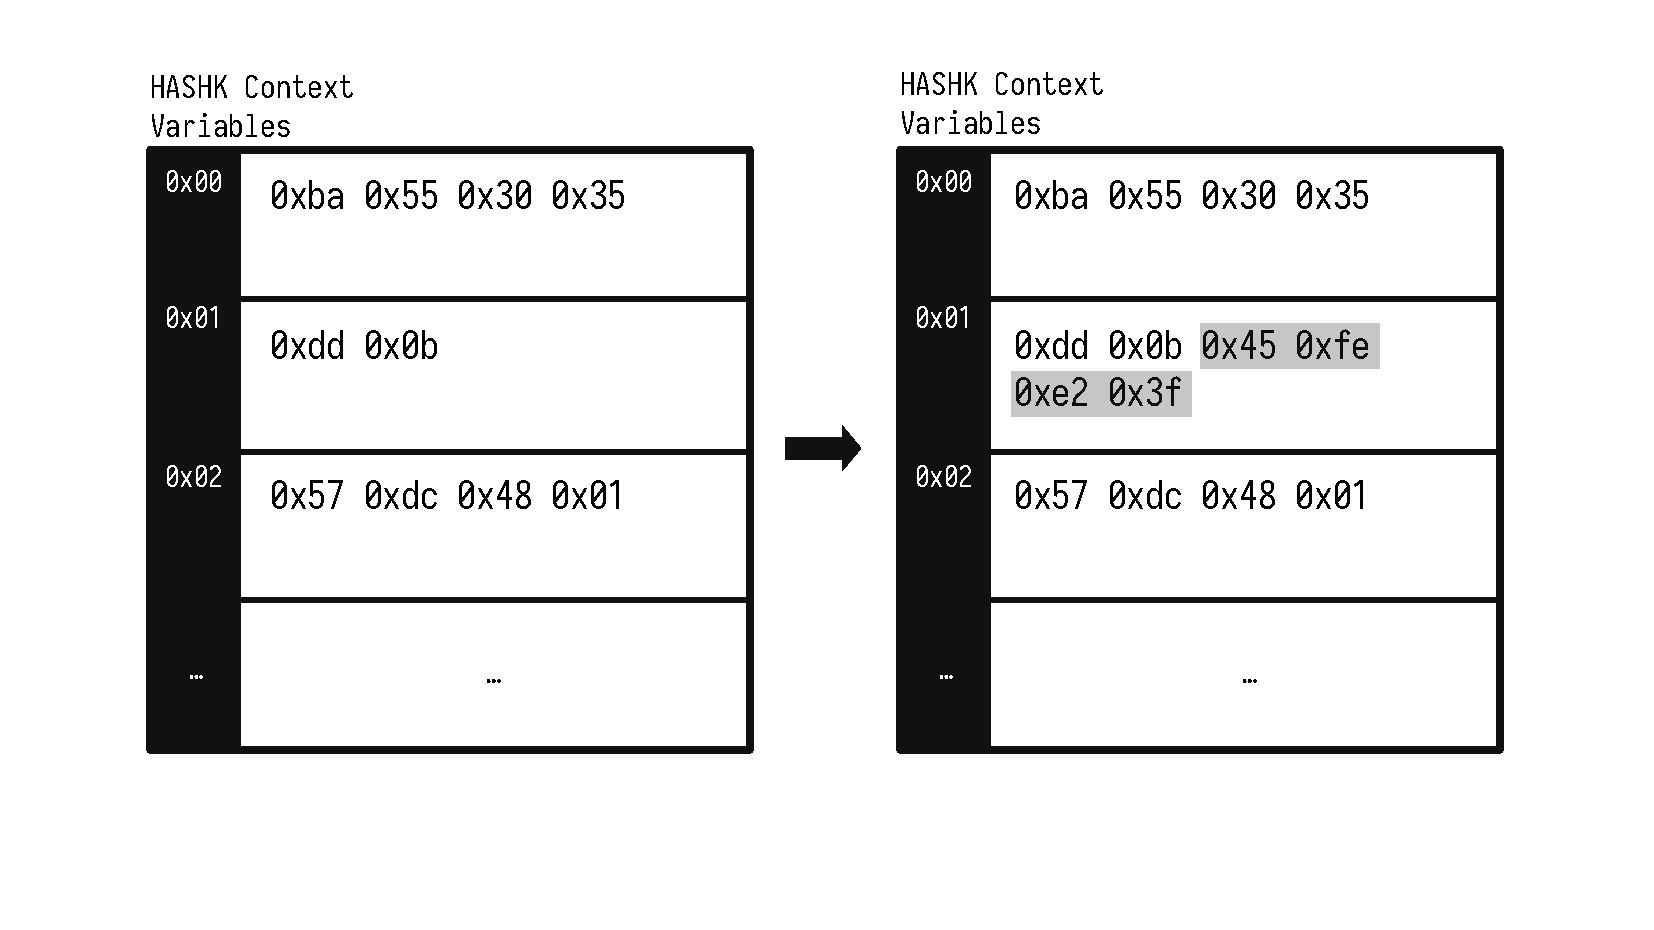
\includegraphics[width=0.6\columnwidth]{\assemblydir/figures/hashk-add-bytes}
    \caption{Schema of the \HASHK instruction.}
    \label{fig:hashk-add-bytes}
\end{figure}

The typical use of the \HASHK instruction in the zkASM language is the following one:

\begin{zkasm}
    op	:HASHK(addr)
\end{zkasm}

The \op placeholder will usually be a register or a register operation like the following one: 

\begin{zkasm}
    A + 1	:HASHK(addr)
\end{zkasm}

We can perform several hashes at the same time, each of them being stored in its corresponding address. Then, we can keep filling each of the addresses' bytes without perturbing the other ones. We can specify the address using the register \E, which is the one used to store addresses $256$-bits, or using a hard coded number. The value $0$ is usually used as an address, which is reserved for storing specific hashes. %TODO: what hashes?

\begin{zkasm}
    A + 1	:HASHK(E)
\end{zkasm}

The former instruction will append the bytes of the current value of \A + 1 into the input of the hash function we want to perform within the bytes attached to the address \E. 

To formalise what the \HASHK instruction does, let $(\op_0, \op_1, \dots, \op_{31})$ be the byte decomposition of the \op variable. We will denote $\mathtt{trunc_{D_0}}(\op)$ by the byte decomposition of \op truncated at the $\mathtt{D_0}$ position. More precisely, 
\[
\mathtt{trunc_{D_0}(\op)} = (\op_0, \op_1, \dots, \op_{\D_0-1}).
\]

Let $\mathtt{hashk}[\texttt{addr}] = (h_0, \dots, h_{\texttt{HASHPOS}})$ be the current array of bytes that we are willing to hash at a certain address \texttt{addr}. The \HASHK instruction will append the $\mathtt{trunc_{D_0}}(\op)$ array into the $\mathtt{hashk}$ one, so that the next state of the (temporal) input of the hash will become 
\[
\mathtt{hashk}[\texttt{addr}] \nextStep = (h_0, \dots, h_{\texttt{HASHPOS}}, \op_0, \op_1, \dots, \op_{\D_0-1})
\]

At the end of this operation, we increase the value of the \texttt{HASHPOS} register in $\mathtt{D_0}$:
\[
\mathtt{HASHPOS} \nextStep = \mathtt{HASHPOS} + \mathtt{D_0}.
\]

Let us propose the following simple example: suppose that we want to hash a single byte concatenated with the first $31$ bytes of a $32$-bytes integer, each of them contained in the registers $\A$ and $\B$ respectively. To that we will use the address \texttt{0x03} stored in the register \E. First of all, we should ensure that our current hash position is $0$, because we are actually starting a new hash.

\begin{zkasm}
    0x03 => E
    0 => HASHPOS
\end{zkasm}

At this moment
\[
\texttt{hashk}[\texttt{0x03}] = \emptyset.
\]

Later on, we will start adding the single byte of \A into the hash input. Observe that we should assign the length $1$ into the register \D because we need to specify the length value in bytes when using the \HASHK instruction. 

\begin{zkasm}
    1 => D
    A				:HASHK(E)
\end{zkasm}

Now, we update the array
\[
\texttt{hashk}[\texttt{0x03}] = (a)
\]
where $a$ denotes the current value of the register \A. Moreover, \texttt{HASHPOS} increased in $1$:
\[
\texttt{HASHPOS} \nextStep = \texttt{HASHPOS} + 1.
\]

Now, we do the same with the register \B

\begin{zkasm}
    31 => D
    B				:HASHK(E)
\end{zkasm}

Finally, the corresponding hash array is the following
\[
\texttt{hashk}[\texttt{0x03}] = (a, b_0, b_1, \dots, b_{30})
\]
where $(b_0, \dots, b_{30}) = \mathtt{trunc}_{31}(\B)$ are the first $31$ bytes of the register \B, which is actually the string we want to hash. Moreover, \texttt{HASHPOS} increased in $31$:
\[
\texttt{HASHPOS} \nextStep = \texttt{HASHPOS} + 31.
\]


\subsubsection{\HASHKONE}

The instruction \HASHKONE performs in the same way that \HASHK but the register $\D_0$ is not relevant here, because the size of the input string is always of $1$ byte. 


\subsubsection{\HASHKLEN}

As commented before, this instruction is actually the one that computes the hash digest and stores it internally, to later on be acquired via the \HASHKDIGEST instruction. This instruction also uses the first $32$ bytes of the \op intermediate value in order to specify the length within all the bytes stored in the specified address that will be hashed. Therefore, the total amount of bytes we can hash is $2^{32}$. 

\begin{figure}[H]
    \centering
    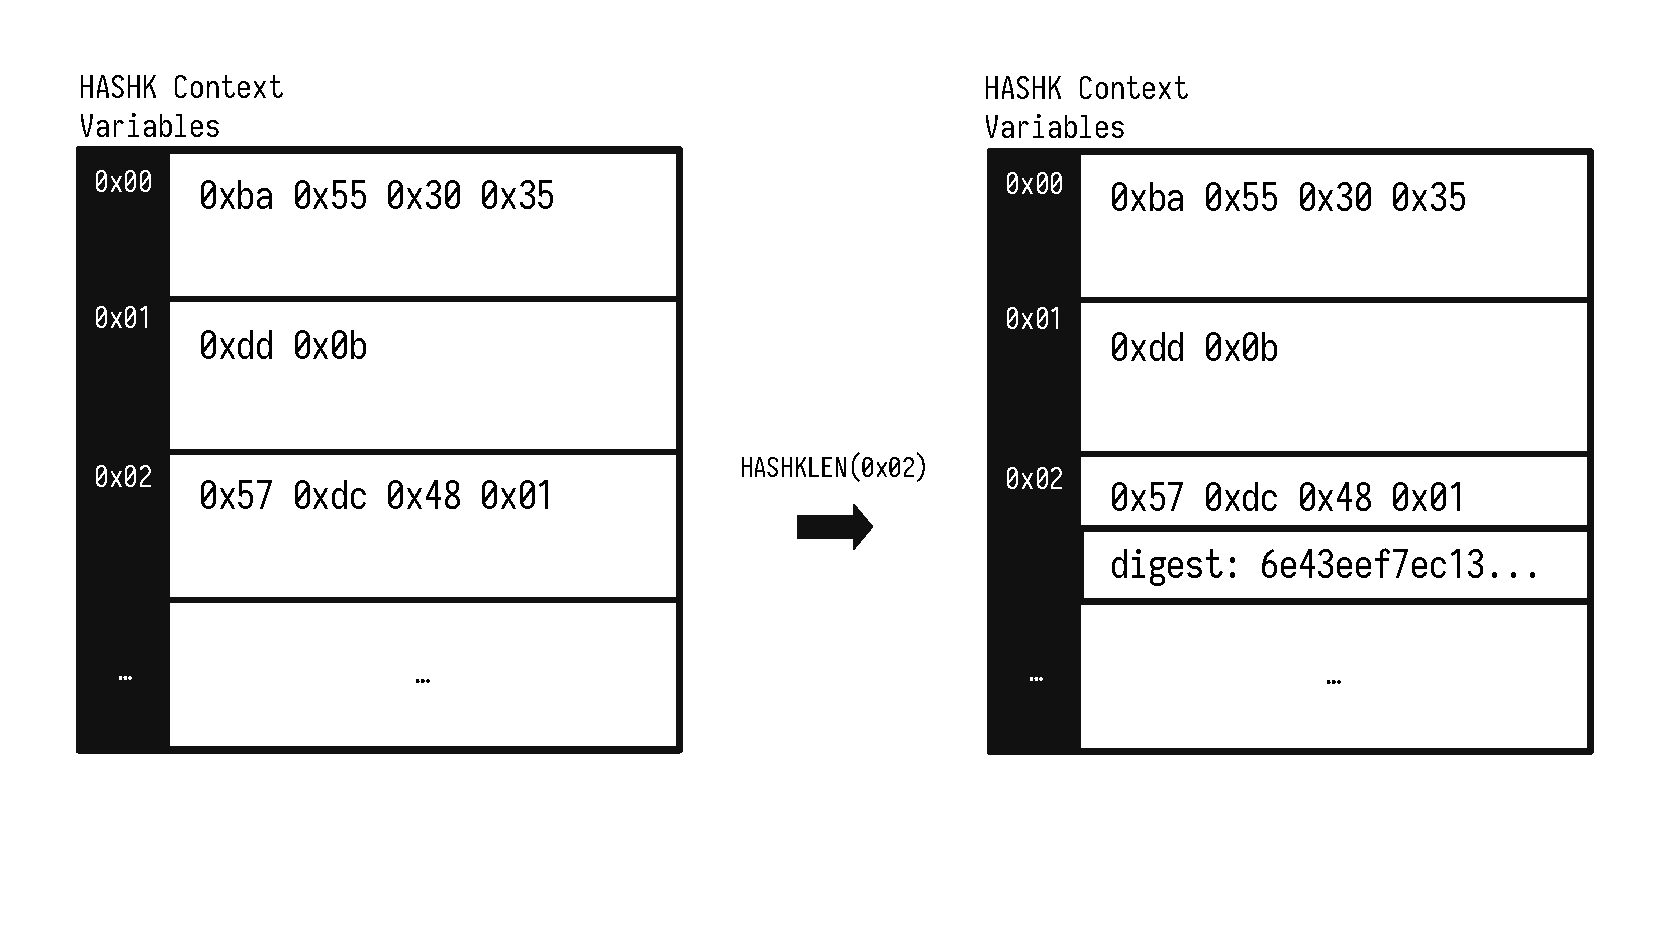
\includegraphics[width=0.6\columnwidth]{\assemblydir/figures/hashklen}
    \caption{Schema of the \HASHKLEN instruction.}
    \label{fig:hashklen}
\end{figure}


Following the previous example, the line of zkASM that we need to execute in this step is the following one:

\begin{zkasm}
    HASHPOS	:HASHKLEN(E)
\end{zkasm}

Recall that \texttt{HASHPOS} value at the current state is $32$ because we want to hash a total amount of $32$ bytes. 


More specifically, if $(h_1, \dots, h_k)$ is the input array attached to a specific address $\texttt{addr}$ (that is, $\mathtt{hashk}[\texttt{addr}] = (h_1, \dots, h_k)$ with the previous notation), the instruction

\begin{zkasm}
    len		:HASHKLEN(addr)
\end{zkasm}

internally stores the digest
\[
d = \texttt{KECCAK-256}(h_1, \dots, h_k).
\]

Observe that we should have that $k = \texttt{len}$. Otherwise, the \HASHKLEN instruction will get an error. % TODO: This checks are checking the integrity of the memory?




\subsubsection{\HASHKDIGEST}

This usual way we are invoking this instruction is the following 

\begin{zkasm}
    $ => REG	:HASHKDIGEST(E)
\end{zkasm}

Meaning that we are storing the digest of the hash attached to the address $\E$ into the register \texttt{REG}. The hash digest is introduced as a free input using the \texttt{\$ =>} operator. In our example, if we want to assign the digest of the hash to the register \D, we would use the following line

\begin{zkasm}
    $ => D		:HASHKDIGEST(E)
\end{zkasm}


%TODO: Counters needs to be incremented.





\newpage
\bibliographystyle{alpha}
\bibliography{../bib/bibliography}


\end{document}


%%%%%%%%%%%%%%%%%%%%%%%%%%%%%%%%%%%%%%%%%%%%%%%%%%%%%%%%%%%%%%%
\section{The Language}


%%%%%%%%%%%%%%%%%%%%%%%%%%%%%%%%%%%%%%%%%%%%%%%%%%%%%%%%%%%%%%%
\subsection{Introduction}

Polynomial Identity Language (PIL) is a novel domain-specific language useful for defining eAIR constraints. The aim of creating PIL is to provide developers with a holistic framework for both constructing programs through an easy-to-use interface and abstracting the complexity of the proving mechanisms.

One of the main peculiarities of PIL is its modularity, which allows programmers to define parametrizable programs, called \texttt{namespaces}, which can be instantiated from larger programs. Building programs in a modular manner makes it easier to test, review, audit and formally verify even large and complex programs. In this regard, by using PIL, developers can create their own custom namespaces or instantiate namespaces from some public library.

Many other domain-specific languages (DSL) or tool stacks, such as Circom or Halo2, focus on the abstraction of a particular computational model, such as an arithmetic circuit. However, recent proof systems such as STARKs have shown that arithmetic circuits might not be the best computational models in all use cases. Given a complete programming language, computing a valid proof for a circuit satisfiability problem, may result in long proving times due to the overhead of re-used logic. Opting for the deployment of programs, with their low-level programming, shorter proving times are attainable, especially with the advent of proof/verification-aiding languages such as PIL.









%%%%%%%%%%%%%%%%%%%%%%%%%%%%%%%%%%%%%%%%%%%%%%%%%%%%%%%%%%%%%%%
\subsection{Creating a Simple Program}\label{sec:simple-program}

To describe the fundamentals of the language itself, let us create a simple PIL program that models the computation of the product of two integers. Consider a program that, at each step, takes two input numbers and multiplies them. Naturally, this program will be referred to as the \Multiplier program. 
% It is important to recall that multiplication is defined over some (large) finite field. 
This program can be modeled using $3$ polynomials: $2$ referring to the inputs that are going to be multiplied $\freeIn_1, \freeIn_2$, and $1$ referring to the output of the computation itself $\out$. As it can be observed, the output column will exhibit a correct behavior if and only if the following identity is satisfied:
\[
\out = \freeIn_1 \cdot \freeIn_2.
\] 

A concrete example of a correct execution trace of the \Multiplier program can be seen in Figure \ref{table:multiplier-ex}. The relation above is satisfied in each of the rows of the execution trace, which means that the output column is filled with correct values. 
\begin{figure}[H]
    \centering
    \begin{tabular}{|c|}
        \hline
        \row\\ \hline
        1			\\
        2			\\
        3			\\
        4			\\
        5			\\
        6			\\
        \vdots			\\
        \hline
    \end{tabular}
    \begin{tabular}{|c|c|c|}
        \hline
        $\freeIn_1$	& $\freeIn_2$		& \out 	\\
        \hline
        4			&2				&8 		\\
        3			&1				&3 		\\
        0			&9				&0  	\\
        7			&3				&21 	\\
        4			&4				&16		\\
        5			&6				&30		\\ 
        \vdots & \vdots & \vdots \\\hline
    \end{tabular}
    \caption{An example of a valid execution trace for the \Multiplier program.}
    \label{table:multiplier-ex}
\end{figure}

%TODO: I think the following is not correct
As it can be seen, there exists a noticeable difference between the behavior of the input columns and the output column which suggests the following classification,
\begin{itemize}
    \item \textbf{Free Input Polynomials:} These are columns that are in charge of introducing the various inputs to the computation. They are referred to as ``free" because at every clocking of the computation, their values do not strictly depend on any previous iteration. These are analogous to independent variables of the entire computation.
    
    \item \textbf{State Variables:} These are the columns that compose the state of the program. Here state refers to the set of values that represent the output of the program at each step and, if we are in the last step, the output of the entire computation.
\end{itemize}




We can now write the corresponding PIL program for the \Multiplier program:
\begin{pil}
    namespace Multiplier(2**10);
    
    // Polynomials
    pol commit freeIn1;
    pol commit freeIn2;
    pol commit out;
    
    // Constraints
    out = freeIn1*freeIn2;
\end{pil}

The reserved keyword \texttt{namespace} is used to frame the scope of the program definition. Inside it, one should define the polynomials used by its program and the constraints among the defined polynomials. A namespace has to be instantiated with a unique name (\Multiplier) together with an argument representing the length of the program, that is, the number of rows (in this case, $2^{10}$) of any execution trace of that program. Besides, the \texttt{commit} keyword allows the compiler to identify the corresponding polynomial as \textbf{committed}. Committed polynomials are opposed to \textbf{constant} polynomials, which are polynomials that are not allowed to change among any execution of the same program. That is, constant polynomials are inherent to the computation itself. This is important from the proving perspective since constant polynomials are publicly known by all parties. However, this is not the case for committed polynomials, which are, in most cases, only known by a party. More on constant polynomials will be added below. 

One should observe that, of course, the former design of the \Multiplier program is not unique. This design is highly not scalable to more complex operations since the number of committed polynomials grows linearly with the number of operations we want to perform. For example, designing a program that computes the result of performing $2^{10}$ operations following the previous design would require $2^{10}$ committed polynomials, which is far from being practical.

However, following another design strategy can easily reduce the $2^{10}$ committed polynomials to a single one by the introduction of another polynomial that flags the starting row of each operation. Together with a third polynomial holding the result of the operation, only a total amount of $3$ columns will be needed. Returning to the initial \Multiplier program, the idea is to introduce a \textbf{constant} polynomial called \RESET that will evaluate to $1$ in odd rows and $0$ otherwise (see Figure \ref{table:multiplier-ex-with-flag}). Nonetheless, this design will also decrease the number of multiplications that can be checked given the same number of rows as the initial design. More concretely, using the initial design we can check one multiplication per row, meanwhile adopting this new strategy will half the number of possible multiplication. 

\begin{figure}[H]
    \centering
    \begin{tabular}{|c|}
        \hline
        \row\\ \hline
        1			\\
        2			\\
        3			\\
        4			\\
        5			\\
        6			\\
        7			\\
        \vdots			\\
        \hline
    \end{tabular}
    \begin{tabular}{|c|c|c|}
        \hline
        \freeIn	&\RESET		&\out 	\\
        \hline
        \textcolor{red}{4}			&1				&0 		\\
        \textcolor{red}{2}			&0				&4 		\\
        \textcolor{orange}{3}			&1				&\textcolor{red}{8}  	\\
        \textcolor{orange}{1}			&0				&3 		\\
        \textcolor{blue}{9}			&1				&\textcolor{orange}{3}		\\
        \textcolor{blue}{0}			&0				&0		\\
        0			&1				&\textcolor{blue}{0}		\\
        \vdots	&\vdots		&\vdots \\ \hline
    \end{tabular}
    \caption{An example of a valid execution trace for the new design of the \texttt{Multiplier} program.}
    \label{table:multiplier-ex-with-flag}
\end{figure}

Observe that, whenever \RESET equals $1$, the value of the \texttt{out} polynomial equals the result of multiplying the previous two values of the \texttt{freeIn} polynomial. In the intermediate steps (that is, when \RESET is equal to $0$), the \texttt{out} polynomial stores the first input of the multiplication. 

Of course, we need to adapt the \Multiplier constraint to reflect the correctness of the \texttt{out} polynomial to the new design. One can observe the following constraint:
\[
\nextStep{\out} = \RESET \cdot \freeIn + (1 - \RESET) \cdot (\out \cdot \freeIn)
\]
completely describes the new design. In PIL, a tick \nextStep{} (which is read ``prime'') over a polynomial is used to denote the value in the next row of such polynomial. In the case of polynomials defined over a multiplicative subgroup $G$ of a prime field $\FF$ with generator $g$, the prime notation is equivalent to the polynomial $\nextStep{\out}(X):= \out(Xg)$.

To see that the previous constraint completely describes our new \Multiplier design, let us distinguish between two cases: 
\begin{itemize}
    \item When \RESET is equal to $1$, the above constraint becomes:
    \[
    \nextStep{\out} = \freeIn.
    \]
    Hence, we are setting the \freeIn polynomial's value in the current row into the \out polynomial's value of the next row.
    
    \item When \RESET is equal to $0$, the above constraint becomes:
    \[
    \nextStep{\out} = \out \cdot \freeIn.
    \]
    Hence, this constraint is stating that the \out polynomial's value in the next row will become the product of the value of \freeIn in the last two rows, the more distance contained in the \out polynomial (as in PIL we are not allowed to access to more than one previous row's values). 
\end{itemize}

The optimized design of the \Multiplier program can be written in PIL as follows:
\begin{pil}
    namespace Multiplier(2**10);
    
    // Constant Polynomials
    pol constant RESET;
    
    // Committed Polynomials
    pol commit freeIn;
    pol commit out;
    
    // Constraints
    out' = RESET*freeIn + (1-RESET)*(out*freeIn);
\end{pil}
Observe that now, the polynomial \RESET is defined with the reserved keyword \texttt{constant}, because it does not change among several executions of the same program. Finally, note that the same design can be extended for a much larger amount of multiplications without needing to modify the PIL itself. Instead, we simply would extend the \RESET polynomial as follows:
\[
\RESET = 
\begin{cases}
    1, & \text{if } i \equiv 0 \pmod{n} \\
    0, & \text{otherwise}
\end{cases}
\]
where $i$ represents the row number (starting from $0$) and $n$ refers to the number of operations.




%%%%%%%%%%%%%%%%%%%%%%%%%%%%%%%%%%%%%%%%%%%%%%%%%%%%%%%%%%%%%%%
\subsection{Compilation}

The previous PIL program is almost ready to be compiled into a JSON file using the \pilcom package \cite{pilcom}. This file is a basic JSON representation of the PIL program (with some extra metadata) that will be consumed later on by the \texttt{pil-stark} package \cite{pilstark} to generate a STARK proof. However, there is a strong restriction when dealing with PIL's constraints. Let $S$ be the set of all polynomials defined over a field $\FF$ appearing in the PIL program. Formally, a constraint is a polynomial identity $f = 0$ where $f \in \FF[S, \nextStep{S}]$ where $\nextStep{S}$ is the set of all the shifted polynomials $p(g X)$ with $p \in S$. The restriction in PIL is the following: \textbf{the degree of $f$ must be less or equal to $2$}.

For example, recall the previous PIL program for the optimized \Multiplier program. The constraint 
\[
\nextStep{\out} = \RESET \cdot \freeIn + (1 - \RESET) \cdot (\out \cdot \freeIn).
\]
can be viewed as the polynomial identity $f = 0$ where $f$ equals to
\[
\nextStep{\out} - \RESET \cdot \freeIn + (1 - \RESET) \cdot (\out \cdot \freeIn)
\]
which belongs to $\FF[\out, \nextStep{\out}, \RESET, \freeIn]$ but \textbf{does not have degree less or equal than $2$}, because it contains the monomial
\[
\RESET \cdot \out \cdot \freeIn.
\]

The idea that PIL has introduced to solve this limitation is to create a new polynomial, conveniently named \texttt{carry}, that will store the product $\out \cdot \freeIn$, that is,
\[
\carry = \out \cdot \freeIn.
\]

This kind of polynomial will be called \textbf{intermediate}. Observe that the prover does not need to provide intermediate polynomials since they can be derived directly from the committed and constant polynomials. Only the way of computing it is strictly necessary. 

Now, the former PIL program can be modified to introduce this newly intermediate \texttt{carry} polynomial:
\begin{pil}
    namespace Multiplier(2**10);
    
    // Constant Polynomials
    pol constant RESET;
    
    // Committed Polynomials
    pol commit freeIn;
    pol commit out;
    
    // Intermediate Polynomials
    pol carry = out*freeIn;
    
    // Constraints
    out' = RESET*freeIn + (1-RESET)*carry;
\end{pil}

At this point, given a (valid) PIL file (ending with the \texttt{.pil} extension) the \pilcom compiler will return a JSON file. %TODO: Add the JSON in the appendix
For example, the \Multiplier program's PIL located in \texttt{multiplier.pil} can be compiled by invoking the following command:

\begin{lstlisting}
    pilcom$ node src/pil.js multiplier.pil -o multiplier.json
\end{lstlisting}

Apart from the JSON file, the compiler will throw a debugging message into the console:

\begin{lstlisting}
    Input Pol Commitments: 2
    Q Pol Commitmets: 1
    Constant Pols: 1
    Im Pols: 1
    plookupIdentities: 0
    permutationIdentities: 0
    connectionIdentities: 0
    polIdentities: 1
\end{lstlisting}

In the previous message, it can be checked that the number of committed polynomials (\texttt{Input Pol Commitments}), the number of constant polynomials (\texttt{Constant Pols}), the number of intermediate polynomials (\texttt{Im Pols}) and the total number of identity constraints (\texttt{polIdentities}) agrees with the corresponding PIL code. 



%TODO: I think we should move this to the connection programs section
Since one of the key features of PIL is that it allows modularity, a dependency inclusion feature among different \texttt{.pil} files have been developed. To briefly show this feature, a configuration \texttt{.pil} file containing the degree bound for polynomials will be created and be used along several PIL programs to remove magic numbers like $2^{10}$. More generically, \texttt{config.pil} will typically include some configuration-related components, shared among various programs. To declare a constant, it can do it using the \texttt{constant} keyword. The compiler distinguishes between constants identifiers and other identifiers (like polynomial identifiers) via the percent \texttt{\%} symbol. Henceforth, constant identifiers should be preceded by the percent symbol. 

\begin{pil}
    // Filename: config.pil
    
    constant %N = 2**10;
\end{pil}

In order to relate both files, the \texttt{include} reserved keyword must be invoked.

\begin{pil}
    // Filename: multiplier.pil
    
    include "config.pil";
    
    namespace Multiplier(%N);
    
    // Constant Polynomials
    pol constant RESET;
    
    // Committed Polynomials
    pol commit freeIn;
    pol commit out;
    
    // Intermediate Polynomials
    pol carry = out*freeIn;
    
    // Constraints
    out' = RESET*freeIn + (1-RESET)*carry;
\end{pil}








%TODO: I think that we can remove this section
%%%%%%%%%%%%%%%%%%%%%%%%%%%%%%%%%%%%%%%%%%%%%%%%%%%%%%%%%%%%%%%
%\subsection{Compiling a Machine (degree 3)}
%
%Suppose now that we are willing to modify the previous program in order not to compute simple multiplications $x \cdot y$ for $x, y \in \FF$ but squared multiplications $x^2 \cdot y^2$. We will call this program \textit{SquareAndMultiply} program. We can model this computation in the same way as before, but modifying the PIL accordingly:
%
%\begin{figure}[H]
%\centering
%\[
%\begin{array}{|c|c|c|}
%\hline
%\freeIn	&\RESET		&\out 	\\
%\hline
%4			&1				&0 		\\
%2			&0				&16		\\
%3			&1				&64  	\\
%1			&0				&9 		\\
%9			&1				&9		\\
%0			&0				&81		\\
%\dots		&\dots			&\dots \\ \hline
%\end{array}
%\]
%\caption{Concrete example of a correct execution of the \texttt{SquareAndMultiply} program.}
%\label{table:multiplier-ex-with-flag2}
%\end{figure}
%
%\begin{pil}
%namespace Multiplier(2**10);
%
%    // Constant Polynomials
%    pol constant RESET;
%
%    // Input Polynomials
%    pol commit freeIn;
%
%    // State Variables
%    pol commit out;
%
%    // Constraints
%    out' = RESET*freeIn*freeIn + (1 - RESET)*(out*freeIn*freeIn);
%\end{pil}
%
%The previous PIL program is almost ready to be compiled into a \texttt{.json} that can be interpreted by the \pilcom package %TODO: Link package
%in order to generate a valid set of polynomials and constraints, which will be used later on by the \texttt{pil-stark} package to generate a valid proof. However, there is a strong restriction when dealing with PIL's constraints. Let $S$ be the set of all polynomials (or equivalently, columns) defined over a field $\FF$ appearing in the PIL program. Formally, a constraint is a polynomial identity $f = 0$ where $f \in \FF[S, \nextStep{S}]$ where $\nextStep{S}$ is the set of all the shifted polynomials $p(g X)$ with $p \in S$. The restriction in PIL is the following: \textbf{the degree of $f$ must be less or equal than $3$}.
%
%For example, recall the previous PIL program for the optimized \Multiplier program. The constraint 
%\[
%    \nextStep{\out} = \RESET \cdot \freeIn \cdot \freeIn + (1 - \RESET) \cdot (\out \cdot \freeIn \cdot \freeIn).
%\]
%can be viewed as the polynomial identity $f = 0$ where $f$ equals to
%\[
%    \nextStep{\out} - \RESET \cdot \freeIn \cdot \freeIn + (1 - \RESET) \cdot (\out \cdot \freeIn \cdot \freeIn)
%\]
%which belongs to $\FF[\out, \nextStep{\out}, \RESET, \freeIn]$ but \textbf{does not have degree less or equal than $3$}, because it contains the monomial
%\[
%\RESET \cdot \out \cdot \freeIn \cdot \freeIn.
%\]
%
%The idea that PIL has introduced to solve this limitation is to create a new polynomial, conveniently named \texttt{square}, that will store the product $\freeIn \cdot \freeIn$, that is,
%\[
%\texttt{square} = \freeIn \cdot \freeIn.
%\]
%
%This kind of polynomials will be called \textbf{intermediate}. Observe that the prover does not need to provide intermediate polynomials since they can be derived directly from the committed and constant polynomials. Only the way of computing is strictly necessary. 
%
%Now, the former PIL program can be modified in order to introduce this newly intermediate \texttt{square} polynomial:
%
%\begin{pil}
%namespace Multiplier(2**10);
%
%    // Constant Polynomials
%    pol constant RESET;
%
%    // Input Polynomials
%    pol commit freeIn;
%
%    // State Variables
%    pol commit out;
%
%    // intermediate Polynomials
%    pol square = freeIn*freeIn;
%
%    // Constraints
%    out' = RESET*square + (1 - RESET)*out*square;
%\end{pil}
%
%At this point, given a (valid) PIL file (ending with the \texttt{.pil} extension) the \pilcom compiler will return a \texttt{.json} file. For example, the Multiplier program's PIL located in \texttt{multiplier.pil} can be compiled by invoking the following command:
%
%\begin{lstlisting}
%pilcom$ node src/pil.js multiplier.pil -o <output.pil.json>
%\end{lstlisting}
%
%Apart from the \texttt{.json} file, the compiler will throw a debugging message into the console:
%
%\begin{lstlisting}
%Input Pol Commitments: 2
%Q Pol Commitmets: 1
%Constant Pols: 1
%Im Pols: 1
%plookupIdentities: 0
%permutationIdentities: 0
%connectionIdentities: 0
%polIdentities: 1
%\end{lstlisting}
%
%In the previous message it can be checked the number of committed polynomials (\texttt{Input Pol Commitments}), the number of constant polynomials (\texttt{Constant Pols}), the number of intermediate polynomials (\texttt{Im Pols}) and the total number of polynomial constraints (\texttt{polIdentities}) used in the compiled PIL code. 
%
%Since one of the key features of PIL is that is allows modularity, a dependency inclusion feature among different \texttt{.pil} files has been developed. In order to briefly show this feature, a configuration \texttt{.pil} file containing the degree bound for polynomials will be created and be used along several PIL programs to remove magic numbers like $2^{10}$. More generically, \texttt{config.pil} will typically include some configuration-related components, shared among various programs. To declare a constant, it can be do it using the \texttt{constant} keyword. The compiler distinguish between constants identifiers and other identifiers (like polynomial identifiers) via the percent \texttt{\%} symbol. Henceforth, constant identifiers should be preceded by the percent symbol. 
%
%\begin{pil}
%// Filename: config.pil
%
%constant %N = 2**10;
%\end{pil}
%
%In order to relate both files, the \texttt{include} reserved keyword must be invoked.
%
%\begin{pil}
%// Filename: multiplier.pil
%
%include "config.pil";
%
%namespace Multiplier(%N);
%
%    pol constant RESET;
%    pol commit freeIn;
%    pol commit out;
%    pol square = freeIn*freeIn;
%    
%    out' = RESET*square + (1 - RESET)*out*square;
%\end{pil}







%%%%%%%%%%%%%%%%%%%%%%%%%%%%%%%%%%%%%%%%%%%%%%%%%%%%%%%%%%%%%%%
\subsection{Cyclic Constraints}

Since execution traces have finite length $N$, there is one implicit complexity in the design of programs with PIL: constraints should be satisfied over every element of a subgroup $G = \Angle{g}$ of $\FF^*$ of size $N$. This means that the description (in terms of constraints) of a program is not correct if the appropriate constraints are not satisfied in every row transition. This is because the polynomials defined from the columns of the execution trace are constructed by interpolation at $G$. In particular, constraints containing polynomials using the prime notation should remain true in the transition from the last row to the first row because $g \cdot g^{N} = g \cdot 1 = g$ (by Lagrange's theorem) and therefore:
\[
\nextStep{p}(g^{N}) = p(g \cdot g^N) = p(g),
\]
which is the first value of the column defined by the polynomial $p$. 

This is an important aspect that has to be taken care of when designing the set of constraints of a program with PIL. If there is some constraint that is not satisfied in the last transition, one normally overcomes this problem by the inclusion of additional polynomials that solve this issue. For example, consider the following PIL code:
\begin{pil}
    namespace CyclicExample(4);
    pol commit a, b;
    
    (a+1)*a*(a-1) = 0;
    b' = b+a;
\end{pil}
and the following valid execution trace:
\begin{figure}[H]
    \centering
    \begin{tabular}{|c|}
        \hline
        \row\\ \hline
        1			\\
        2			\\
        3			\\
        4			\\
        \hline
    \end{tabular}
    \begin{tabular}{|c|c|}
        \hline
        \att	&\btt \\ \hline
        1			&1			\\
        0			&2			\\
        -1			&2			\\
        1			&1			\\
        \hline
    \end{tabular}
\end{figure}

Observe that the polynomial \att only takes the values $0, 1$ or $-1$ (equivalently, $p-1$) and this is precisely captured by the constraint: 
\[
(\att+1) \cdot \att \cdot (\att-1) = 0,
\]
which is satisfied for each row $i \in [4]$.

On the other side, the second constraint $\nextStep{\btt} = \btt + \att$ is satisfied for every row except for the last, because: 
\begin{equation}\label{eq:cyclic}
    \nextStep{\btt}(g^4) = \btt(1) = 1 \neq 2 = 1 + 1 = \btt(g^4) + \att(g^4),
\end{equation}
where $g$ is the generator of the group $G$ of size $4$.

The idea to overcome this problem is to add a constant column \SEL that is $1$ in every row except for the last one and introduce it to the previous constraint as follows:
\[
\btt' = \SEL \cdot (\btt+\att) + (1-\SEL).
\]
Notice that now the right-hand side of Eq. \eqref{eq:cyclic} is equal to $\SEL(g^4) \cdot (\btt(g^4) + \att(g^4)) + (1-\SEL(g^4)) = 1$.

The valid PIL is the following:
\begin{pil}
    namespace CyclicExample(4);
    
    pol commit a, b;
    pol constant SEL;
    pol carry = (a+1)*a;
    
    carry*(a-1) = 0;
    b' = SEL*(b+a) + (1-SEL);
\end{pil}








%%%%%%%%%%%%%%%%%%%%%%%%%%%%%%%%%%%%%%%%%%%%%%%%%%%%%%%%%%%%%%%
\subsection{Inclusion Arguments}

There is a subtlety in the \Multiplier example of Section \ref{sec:simple-program} that is worth commenting on at this point. It is assumed that columns can contain field elements but, it may be the case where one needs to restrict the size of the columns' values to a certain number of bits. Henceforth, it is important to develop a strategy to control both underflows and overflows. In this section, we will design a program (and its corresponding PIL) to verify the addition of two integers of a size fitting in exactly $2$ bytes. That is, any input to the addition will be considered invalid if it is not an integer in the range $[0,65535]$.

Of course, there is plenty of ways to arithmetize this program. However, in this section, we are going to use a method based on inclusion arguments. The overall idea is to reduce $2$-byte additions to $1$-byte additions. Specifically, the program will consist of two input polynomials \att and \btt where each one will, at each row, introduce a single byte (equivalently, an integer in the range $[0,255]$) for each operand of the sum, starting with the less significant byte. Hence, every two rows, a new addition will be checked.
\begin{figure}[H]
    \centering
    \begin{tabular}{|c|}
        \hline
        \row\\ \hline
        1			\\
        2			\\
        3			\\
        4			\\
        \hline
    \end{tabular}
    \begin{tabular}{|c|c|c|}
        \hline
        \att		&\btt		& \texttt{operation} \\
        \hline
        \texttt{0x11}	&\texttt{0x22}	&\textit{undefined}\\
        \texttt{0x30}	&\texttt{0x40}	&\texttt{0x3011} + \texttt{0x4022}\\
        \texttt{0xff}	&\texttt{0xee}	&\textit{undefined}\\
        \texttt{0x00}	&\texttt{0xff}	&\texttt{0x00ff} + \texttt{0xffee}\\
        \hline
    \end{tabular}
    \label{table:2-bytes-sum-sm}
\end{figure}

The output of the addition between words of $1$-byte can not be stored in a single column that only accepts words of $1$-byte, since an overflow may appear. Hence, the result of the addition will be split into two columns \texttt{carry} and \add, accepting words of exactly $1$-byte, to completely store the result so that a correct addition between bytes can be defined as:
\begin{equation}
    \label{byte-sum-carry}
    \att + \btt = \carry \cdot 2^8 + \add.
\end{equation}

Table \ref{table:2-bytes-sum-carry-add} shows an example of a valid execution trace for this program. Note that the result of operating each of the $2$-bytes words can be obtained by simply grabbing the value in the last \texttt{carry} value and each of the last two \add's values in decreasing order. For example, $\mathtt{0x3011} + \mathtt{0x4022} = \mathtt{0x007033}$, which can be recovered from the blue cells below. The same applies for $\mathtt{0x00ff} + \mathtt{0xffee} = \mathtt{0x0100ed}$, which can be recovered similarly from the pink cells. 

\begin{table}[H]
    \centering
    \begin{tabular}{|c|}
        \hline
        \row\\ \hline
        1			\\
        2			\\
        3			\\
        4			\\
        \hline
    \end{tabular}
    \begin{tabular}{|c|c|c|c|}
        \hline
        \att		&\btt		&\carry		&\add 	\\
        \hline
        \texttt{0x11}	&\texttt{0x22}	&\texttt{0x00}		&\cellcolor{cyan} \texttt{0x33} 	\\
        \texttt{0x30}	&\texttt{0x40}	&\cellcolor{cyan} \texttt{0x00}		&\cellcolor{cyan} \texttt{0x70}	\\ \hline
        \texttt{0xff}	&\texttt{0xee}	&\texttt{0x01}		&\cellcolor{pink} \texttt{0xed}  \\
        \texttt{0x00}	&\texttt{0xff}	&\cellcolor{pink} \texttt{0x01}		&\cellcolor{pink} \texttt{0x00}	\\
        \hline
    \end{tabular}
    \caption{TBD}
    \label{table:2-bytes-sum-carry-add}
\end{table}

One can notice that constraint \eqref{byte-sum-carry} is not satisfied at row $4$, because the \carry's value that is raised in the third row must be introduced into the $1$-byte addition at row $4$. In this way, we can link the two-byte sums that compose $2$-byte additions. There is no direct way to introduce the previous row of a column in PIL (in contrast with the next row, which we can invoke with the single quote operator \nextStep{}). The idea then is to introduce another committed polynomial called \texttt{prevCarry} which will contain a shifted version of the value in the  \texttt{carry} polynomial. More specifically, we add the following constraint to ensure that \texttt{prevCarry} is correctly defined:
\begin{equation}\label{eq:carries}
    \mathtt{prevCarry}' = \carry
\end{equation}

\begin{figure}[H]
    \centering
    \begin{tabular}{|c|}
        \hline
        \row\\ \hline
        1			\\
        2			\\
        3			\\
        4			\\
        \hline
    \end{tabular}
    \begin{tabular}{|c|c|c|c|c|}
        \hline
        \att		&\btt		&\texttt{prevCarry}		&\carry	&\add 	\\
        \hline
        \texttt{0x11}	&\texttt{0x22}	&\texttt{0x01}		&\texttt{0x00}		&\texttt{0x33} 	\\
        \texttt{0x30}	&\texttt{0x40}	&\texttt{0x00}		&\texttt{0x00}		&\texttt{0x70}	\\ \hline
        \texttt{0xff}	&\texttt{0xee}	&\texttt{0x00}		&\texttt{0x01}		&\texttt{0xed}  \\
        \texttt{0x00}	&\texttt{0xff}	&\texttt{0x01}		&\texttt{0x01}		&\texttt{0x00}	\\
        \hline
    \end{tabular}
    \label{table:2-bytes-sum-prev-carry}
\end{figure}

Now we face another problem: the previous carry must not affect two different 2-byte additions as per constraint \eqref{eq:carries}. That is, non-related operations should not be linked via carries. Henceforth, a constant polynomial called \RESET will be introduced to break the present connection between different additions. The \RESET polynomial will be a binary-ranged polynomial which will be $1$ at the beginning of every $2$ byte addition. Elsewhere, \RESET will evaluate to $0$. 

\begin{figure}[H]
    \centering
    \begin{tabular}{|c|}
        \hline
        \row\\ \hline
        1			\\
        2			\\
        3			\\
        4			\\
        \hline
    \end{tabular}
    \begin{tabular}{|c|c|c|c|c|c|c}
        \hline
        \att		&\btt		&\texttt{prevCarry}	&\carry		&\add		&\RESET 	\\
        \hline
        \texttt{0x11}	&\texttt{0x22}	&\texttt{0x01}		&\texttt{0x00}		&\texttt{0x33}		&1 					\\
        \texttt{0x30}	&\texttt{0x40}	&\texttt{0x00}		&\texttt{0x00}		&\texttt{0x70}		&0					\\ \hline
        \texttt{0xff}	&\texttt{0xee}	&\texttt{0x00}		&\texttt{0x01}		&\texttt{0xed}		&1  				\\
        \texttt{0x00}	&\texttt{0xff}	&\texttt{0x01}		&\texttt{0x01}		&\texttt{0x00}		&0					\\
        \hline
    \end{tabular}
    \label{table:2-bytes-sum-reset}
\end{figure}

Following this logic, we can now derive the final (and accurate) constraint: 
\begin{equation}
    \label{byte-sum-pil}
    \att + \btt + (1 - \RESET) \cdot \mathtt{prevCarry} = \carry \cdot 2^8 + \add.
\end{equation}

The PIL program of the previous example can be written as follows:
\begin{pil}
    include "config.pil";
    
    namespace TwoByteAdd(%N);
    
    pol constant RESET;
    pol commit a, b;
    pol commit carry, prevCarry, add;
    
    prevCarry' = carry;
    a + b + (1-RESET)*prevCarry = carry*2**8 + add;
\end{pil}

% Observe that the constraint $(1 - \RESET)\cdot\RESET = 0$ has been added in order to enforce \RESET to be binary. 
Similarly to the \Multiplier example of Section \ref{sec:simple-program}, it is worth mentioning that only by changing the \RESET polynomial (but not the PIL itself), it is possible to arithmetize a program being able to verify generic $n$-bytes additions. In such case, \RESET will be $1$ for every $n$ row and $0$ otherwise. 

Up to this point, one can think that Constraint \eqref{byte-sum-pil} restricts a sound representation of the program. However, since we are working over a finite field, it is not. For example, the following execution trace is valid, as it satisfies all the constraints, but does not correspond to a valid computation:
\begin{figure}[H]
    \centering
    \begin{tabular}{|c|}
        \hline
        \row\\ \hline
        1			\\
        2			\\
        3			\\
        4			\\
        \hline
    \end{tabular}
    \begin{tabular}{|c|c|c|c|c|c|c}
        \hline
        \att		&\btt		&\texttt{prevCarry}					&\carry		&\add								&\RESET 	\\
        \hline
        \texttt{0x11}	&\texttt{0x22}	&\texttt{0x01}						&$p \cdot 2^{-8}$					&\texttt{0x33}					&1 					\\
        \texttt{0x30}	&\texttt{0x40}	&$p \cdot 2^{-8}$						&\texttt{0x00}					&$\texttt{0x70} + p \cdot 2^{-8}$	&0					\\ \hline
        \texttt{0xff}	&\texttt{0xee}	&\texttt{0x00}						&$\texttt{0x01} + p \cdot 2^{-8}$	&\texttt{0xed}					&1  				\\
        \texttt{0x00}	&\texttt{0xff}	&$\texttt{0x01} + p \cdot 2^{-8}$		&\texttt{0x01}					&$\texttt{0x00}+ p \cdot 2^{-8}$	&0					\\
        \hline
    \end{tabular}
    \caption{Concrete example showing how to cheat the current program restrictions. }
    \label{table:2-bytes-sum-wrong}
\end{figure}

Moreover, nothing is preventing the introduction of more bytes in either column \a or \b, which breaks the intention of this program, specially designed to deal only with byte-sized columns. Enforcing that all the evaluations of committed polynomials are correct is strictly necessary. As explained at the beginning of this section, an inclusion argument will be used.  

\begin{definition}[Inclusion Argument]
    Given two vectors $a = (a_1, \dots, a_n) \in \FF_p^n$ and $b = (b_1, \dots, b_m) \in \FF_p^m$, we say that \textit{$a$ is contained in $b$} if for all $i \in [n]$, there exists a $j \in [m]$ such that $a_i = b_j$. In words, if we see $a$ and $b$ as multisets and then we reduce them to sets (by removing the multiplicity), then $a$ is contained in $b$ if $a$ is a subset of $b$.
    
    Moreover, we say that a protocol $(\P,\V)$ is an \textit{inclusion argument} if the protocol can be used by $\P$ to prove to $\V$ that one vector is contained in another vector.
\end{definition}

% An inclusion argument is a constraint defined in PIL that is used to check whether $\att \subset \btt$ where \att and \btt are two columns. Since polynomials can be described as vectors via the usual Fourier transform procedure, the following definition can be naturally extended to columns. It is important to observe that $n$ can be less, equal or bigger than $m$ and the former definition still makes sense. Later on, a more restrictive constraint will be introduced.

In the PIL context, the implemented inclusion argument is the inclusion argument provided here \cite{EPRINT:GabWil20}, with the ``alternating method''  provided in \cite{EPRINT:PFMBM22} and can be invoked via the \textsf{in} keyword. Specifically, given two columns \att, \btt, we can declare an inclusion argument between them using the syntax $\{\att\} \textsf{ in } \{\btt\}$, where \att, \btt does not necessarily need to be defined in different programs. See for example:
\begin{pil}
    include "config.pil";
    
    namespace A(%N);
    pol commit a, b;
    
    {a} in {b};
    
    namespace B(%N);
    pol commit a, b;
    
    {a} in {Example1.b};
\end{pil}
A valid execution trace (with $N=4$) for the previous example is shown in Table \ref{table:is-example-1}.
\begin{table}[H]
    \centering
    \begin{tabular}{|c|c|}
        \hline
        \multicolumn{2}{|c|}{\textbf{Program A}} \\
        \hline
        \att	&\btt	\\ \hline
        3	&1	\\
        4	&2 \\
        2	&3\\
        3	&4 \\
        \hline
    \end{tabular}
    \begin{tabular}{|c|c|}
        \hline
        \multicolumn{2}{|c|}{\textbf{Program B}} \\
        \hline
        \att	&\btt	\\ \hline
        1	&6 \\
        1	&7 \\
        1	&8 \\
        4	&9 \\
        \hline
    \end{tabular}
    \caption{Execution traces for programs \textsf{A} and \textsf{B}. }
    \label{table:is-example-1}
\end{table}

In PIL we can also write inclusion arguments not only over single columns but over multiple columns. That is, given two subsets of committed columns $\att_1,\dots,\att_m$ and $\btt_1,\dots,\btt_m$ of some program(s) we can write $\{\att_1,\dots,\att_m\} \texttt{ in } \{\btt_m,\dots,\btt_m\}$ to denote that the rows generated by columns $\btt_m,\dots,\btt_m$ are included (as sets) into the rows generated by columns $\{\att_1,\dots,\att_m\}$. A natural application for this generalization is showing that a set of columns in a program repeatedly computes, probably with the same pair of inputs/outputs, an operation such as $\AND$, where the correct $\AND$ operation is carried on a distinct program (see the following example).
\begin{pil}
    include "config.pil";
    
    namespace Main(%N);
    pol commit a, b, c;
    
    {a,b,c} in {in1,in2,xor};
    
    namespace AND(%N);
    pol constant in1, in2, and;
\end{pil}

%TODO: We should mention that we can add selectors

Following with the previous example, the idea will be to construct $4$ new constant polynomials $\mathtt{BYTE\_A}$, $\mathtt{BYTE\_B}$, $\mathtt{BYTE\_CARRY}$ and $\mathtt{BYTE\_ADD}$ which contain all possible byte additions. The execution trace of these polynomials can be constructed as follows:
\begin{figure}[H]
    \centering
    \begin{tabular}{|c|}
        \hline
        \row\\ \hline
        1			\\
        2			\\
        3			\\
        \vdots			\\
        256			\\
        257			\\
        258			\\
        \vdots			\\
        65535		\\
        65536			\\
        \hline
    \end{tabular}
    \begin{tabular}{|c|c|c|c|}
        \hline
        \texttt{BYTE\_A}	&\texttt{BYTE\_B}	&\texttt{BYTE\_{CARRY}}	&\texttt{BYTE\_{ADD}} \\
        \hline
        \texttt{0x00}		&\texttt{0x00}		&\texttt{0x00}			&\texttt{0x00}		  \\
        \texttt{0x00}		&\texttt{0x01}		&\texttt{0x00}			&\texttt{0x01}		  \\
        \texttt{0x00}		&\texttt{0x02}		&\texttt{0x00}			&\texttt{0x02}		  \\
        \vdots				&\vdots				&\vdots					&\vdots		         \\	
        \texttt{0x00}		&\texttt{0xff}		&\texttt{0x00}			&\texttt{0xff}		  \\
        \texttt{0x01}		&\texttt{0x00}		&\texttt{0x00}			&\texttt{0x01}		  \\
        \texttt{0x01}		&\texttt{0x01}		&\texttt{0x00}			&\texttt{0x02}		  \\
        \vdots				&\vdots				&\vdots					&\vdots				  \\
        \texttt{0xff}		&\texttt{0xfe}		&\texttt{0x01}			&\texttt{0xfd}		  \\
        \texttt{0xff}		&\texttt{0xff}		&\texttt{0x01}			&\texttt{0xfe}		  \\
        \hline
    \end{tabular}
    \caption{Summary of the values for the constant polynomials in the \textsf{TwoByteAdd} program.}
    \label{table:2-bytes-sum-const}
\end{figure}
Recall that enforcing constraints between these polynomials will not be needed since they are constant and therefore, publicly known. 

%TODO: Why doing 4 inclusions is not enough? discuss it
Ensuring that the tuple $(\att, \btt, \carry, \add)$ is contained in the previous table via an inclusion argument will ensure a sound description of the program. The inclusion constraint is not only ensuring that all the values are single bytes, but also checking that the addition is correctly computed. Consequently, none of the rows of Table \ref{table:2-bytes-sum-wrong} is contained in the previous table, marking them as non-valid rows. Of course, this will introduce some redundancy into the PIL, because the byte operation is being checked twice (one with the polynomial constraint and the other with the inclusion argument). However, we can not simply drop the polynomial constraint because it is necessary for linking rows belonging to the same addition. 

The following line of code completes the PIL for the \textsf{TwoByteAdd} program:
\begin{pil}
    {a, b, carry, add} in {BYTE_A, BYTE_B, BYTE_CARRY, BYTE_ADD};
\end{pil}

%TODO: This is not necessary
% We have to take into account that every time an inclusion check is performed in PIL, by requirements of the STARK proof generated by the \texttt{pil-stark} package, a new polynomial $L_1$ (which stands for the first Lagrange polynomial) should be added under the \texttt{Global} namespace. This polynomial is $1$ at the first row and $0$ otherwise. 

% \begin{pil}
    % // Filename: global.pil
    
    % namespace Global(%N);
    %     pol constant L1;
    % \end{pil}

To sum up, the following PIL program correctly describes the \textsf{TwoByteAdd} program:
\begin{pil}
    include "config.pil";
    
    namespace TwoByteAdd(%N);
    
    pol constant BYTE_A, BYTE_B, BYTE_CARRY, BYTE_ADD;
    pol constant RESET;
    pol commit a, b;
    pol commit carry, prevCarry, add;
    
    prevCarry' = carry;
    a + b + (1 - RESET)*prevCarry = carry*2**8 + add;
    
    {a, b, carry, add} in {BYTE_A, BYTE_B, BYTE_CARRY, BYTE_ADD};
\end{pil}

Compiling this $\mathtt{.pil}$ file, we get the following debugging message:
\begin{lstlisting}
    Input Pol Commitmets: 5
    Q Pol Commitmets: 0
    Constant Pols: 5
    Im Pols: 0
    plookupIdentities: 1
    permutationIdentities: 0
    connectionIdentities: 0
    polIdentities: 3
\end{lstlisting}

Observe that $\mathtt{plookupIdentities}$ counts the number of inclusion arguments used in the PIL program (one in our example). 

%%%%%%%%%%%%%%%%%%%%%%%%%%%%%%%%%%%%%%%%%%%%%%%%%%%%%%%%%%%%%%%%%%%5
\subsubsection{Avoiding Redundancy}

Further modifications can be added to avoid redundancy in the PIL. This can be achieved by introducing another constant polynomial $\mathtt{BYTE\_PREVCARRY}$. In this case, the constant polynomials table formed by the polynomials $\mathtt{BYTE\_A}, \mathtt{BYTE\_B}, \mathtt{BYTE\_PREVCARRY}, \mathtt{BYTE\_CARRY}$ and $\mathtt{BYTE\_ADD}$ should be generated by iterating among all the possible combinations of the tuple $(\mathtt{BYTE\_A}, \mathtt{BYTE\_B}, \mathtt{BYTE\_PREVCARRY})$ and computing $\mathtt{BYTE\_CARRY}$ and $\mathtt{BYTE\_ADD}$ accordingly in each of the combinations. The table only becomes twice bigger because \texttt{BYTE\_PREVCARRY} is binary. A summary of how the table looks like with the new changes can be found in Figure \ref{table:2-bytes-sum-const-prevcarry}. 

\begin{figure}[h!]
    \centering
    \begin{tabular}{|c|}
        \hline
        \row\\ \hline
        1			\\
        2			\\
        3			\\
        \vdots			\\
        256			\\
        257			\\
        258			\\
        \vdots			\\
        65535			\\
        65536			\\
        65537			\\
        65538			\\
        65539			\\
        \vdots			\\
        65792		\\
        65793	\\
        65794	\\
        \vdots      \\
        131071		\\
        131072			\\
        \hline
    \end{tabular}
    \begin{tabular}{|c|c|c|c|c|}
        \hline
        \texttt{BYTE\_A}	&\texttt{BYTE\_B}	&\texttt{BYTE\_PREVCARRY}	&\texttt{BYTE\_{CARRY}}	&\texttt{BYTE\_{ADD}} \\
        \hline
        \texttt{0x00}		&\texttt{0x00}		&\texttt{0x00}				&\texttt{0x00}			&\texttt{0x00}		  \\
        \texttt{0x00}		&\texttt{0x01}		&\texttt{0x00}				&\texttt{0x00}			&\texttt{0x01}		  \\
        \texttt{0x00}		&\texttt{0x02}		&\texttt{0x00}				&\texttt{0x00}			&\texttt{0x02}		  \\
        \vdots				&\vdots				&\vdots						&\vdots					&\vdots		         \\	
        \texttt{0x00}		&\texttt{0xff}		&\texttt{0x00}				&\texttt{0x00}			&\texttt{0xff}		  \\
        \texttt{0x01}		&\texttt{0x00}		&\texttt{0x00}				&\texttt{0x00}			&\texttt{0x01}		  \\
        \texttt{0x01}		&\texttt{0x01}		&\texttt{0x00}				&\texttt{0x00}			&\texttt{0x02}		  \\
        \vdots				&\vdots				&\vdots						&\vdots					&\vdots				  \\
        \texttt{0xff}		&\texttt{0xfe}		&\texttt{0x00}				&\texttt{0x01}			&\texttt{0xfd}		  \\
        \texttt{0xff}		&\texttt{0xff}		&\texttt{0x00}				&\texttt{0x01}			&\texttt{0xfe}		  \\
        \texttt{0x00}		&\texttt{0x00}		&\texttt{0x01}				&\texttt{0x00}			&\texttt{0x00}		  \\
        \texttt{0x00}		&\texttt{0x01}		&\texttt{0x01}				&\texttt{0x00}			&\texttt{0x02}		  \\
        \texttt{0x00}		&\texttt{0x02}		&\texttt{0x01}				&\texttt{0x00}			&\texttt{0x03}		  \\
        \vdots				&\vdots				&\vdots						&\vdots					&\vdots		         \\	
        \texttt{0x00}		&\texttt{0xff}		&\texttt{0x01}				&\texttt{0x01}			&\texttt{0x00}		  \\
        \texttt{0x01}		&\texttt{0x00}		&\texttt{0x01}				&\texttt{0x00}			&\texttt{0x02}		  \\
        \texttt{0x01}		&\texttt{0x01}		&\texttt{0x01}				&\texttt{0x00}			&\texttt{0x03}		  \\
        \vdots				&\vdots				&\vdots						&\vdots					&\vdots				  \\
        \texttt{0xff}		&\texttt{0xfe}		&\texttt{0x01}				&\texttt{0x01}			&\texttt{0xfe}		  \\
        \texttt{0xff}		&\texttt{0xff}		&\texttt{0x01}				&\texttt{0x01}			&\texttt{0xff}		  \\
        \hline
    \end{tabular}
    \caption{Summary of the values for the constant polynomials adding \texttt{BYTE\_PREVCARRY}.}
    \label{table:2-bytes-sum-const-prevcarry}
\end{figure}


In addition, recall that we only have to take into account \texttt{prevCarry} whenever \RESET is $0$. PIL is flexible enough to consider this kind of situation involving Plookups. To introduce this requirement, the inclusion check can be modified as follows:
\begin{pil}
    {a, b, (1 - RESET)*prevCarry, carry, add} in {BYTE_A, BYTE_B, BYTE_PREVCARRY, BYTE_CARRY, BYTE_ADD};
\end{pil}

With this modification, the PIL program becomes:
\begin{pil}
    include "config.pil";
    
    namespace TwoByteAdd(%N);
    
    pol constant BYTE_A, BYTE_B, BYTE_PREVCARRY, BYTE_CARRY, BYTE_ADD;
    pol constant RESET;
    pol commit a, b;
    pol commit carry, prevCarry, add;
    
    prevCarry' = carry;
    
    {a, b, (1 - RESET)*prevCarry, carry, add} in {BYTE_A, BYTE_B, BYTE_PREVCARRY, BYTE_CARRY, BYTE_ADD};
\end{pil}


%TODO: Which of the solutions is better?




%TODO: This whole example needs to be changed
%%%%%%%%%%%%%%%%%%%%%%%%%%%%%%%%%%%%%%%%%%%%%%%%%%%%%%%%%%%%%%%
\subsection{Connecting Programs} \label{sec:connecting-sm}

One of the core features of PIL is that it allows a \textit{modular design} of its programs. By modular we mean the ability to split the design of a program $M$ in multiple small programs such that the (proper) combination of the small programs lead to $M$. 
% Modularity provides us with a framework to connect several programs that prevent them to overgrow. 
Without this feature, one would need to combine the logic of multiple pieces in a single design and, as a consequence, a lot of redundant polynomials would be included in the design. Moreover, the resulting big design would be difficult to validate and test. 

Through this section, the modularity feature will be shown using the following example. Suppose that we want to design a program to verify the operation $a \cdot \overline{a}$, where $a$ is a $4$-bits integer and $\overline{a}$ is defined as the integer obtained by negating each of the bits of $a$ (i.e., $\overline{a}$ is the bitwise negation of $a$). The difficulty here is that bitwise operations are difficult to describe when working directly with chunks of $4$-bits. Then, the idea will be to split them into bits in another program, allowing us to check the operations in a trivial way. 

The main program will consist in $3$ columns: \att, \texttt{neg\_a} and \texttt{op}. The column \att will contain at each row the integer $a$ of the computation $a \cdot \overline{a}$. The columns \texttt{neg\_a} and \texttt{op} will contain $\overline{a}$ and $a \cdot \overline{a}$, respectively. Table \ref{table:connecting-sm-main} represents a valid execution trace of the program.
\begin{table}[H]
    \centering
    \begin{tabular}{|c|}
        \hline
        \row\\ \hline
        1			\\
        2			\\
        3			\\
        4           \\
        \hline
    \end{tabular}
    \begin{tabular}{|c|c|c|}
        \hline
        \att	&\texttt{neg\_a}	&\texttt{op} 	\\ \hline
        1101		&0010				&00011010		\\
        0100		&1011				&00101100		\\
        1111		&0000				&00000000		\\
        1000		&0111				&00111000		\\
        \hline
    \end{tabular}
    \caption{Concrete example of the program that validates negated strings of bits. }
    \label{table:connecting-sm-main}
\end{table}

First, there is the need to enforce that each of the inputs is effectively a $4$-bits integer (that is, an integer in the range $[0,15]$). This can be enforced via an inclusion argument. Specifically, this argument enforces that all the values of a vector belong to a certain (publicly known) range. For this reason, this family of inclusion arguments is often referred to as \textit{range checks}. The PIL code for the range check for column \att is as follows:
\begin{pil}
    include "config.pil";
    
    namespace Global(%N);
    pol constant BITS4;
    
    namespace Main(%N);
    pol commit a, neg_a, op;
    
    a in Global.BITS4;
\end{pil}

There are two important remarks about the former PIL code. First, \texttt{BITS4} is a polynomial containing each one of the possible $4$-bits integers. Any order can be chosen to construct it because inclusion checks do not care about the ordering. Second, observe that \texttt{BITS4} is called from a different namespace where it is defined. The syntax \texttt{Namespace.polynomial} can be used to access other's namespaces polynomials. The idiomatic way of proceeding is to put different namespaces in separated files and then use the \texttt{include} keyword to ``connect'' them:
\begin{pil}
    // Filename: global.pil
    
    include "config.pil";
    
    namespace Global(%N);
    pol constant L1;
    pol constant BITS4;
\end{pil}

\begin{pil}
    // Filename: main.pil
    
    include "config.pil";
    include "global.pil"
    
    namespace Main(%N);
    pol commit a, neg_a, op;
    
    a in Global.BITS4;
\end{pil}

As mentioned before, working with $4$ bits directly would be difficult. Hence, another program that works bitwise will be designed. This program will contain a column \bits that will store the single bits that shape each of the integers present in $a$ in expressed as little-endian. Similarly, a column \nbits will contain the negation of each one of the previous bits. For a concrete example of the execution trace, see Table \ref{table:connecting-sm-bits}. 

\begin{figure}[h!]
    \centering
    \begin{tabular}{|c|}
        \hline
        \row\\ \hline
        1			\\
        2			\\
        3			\\
        4           \\
        5			\\
        6			\\
        7			\\
        8           \\
        \vdots      \\
        \hline
    \end{tabular}
    \begin{tabular}{|c|c|c|}
        \hline
        \bits	&\nbits &\FACTOR	\\  \hline
        1				&0				&1				\\
        0				&1				&2				\\
        1				&0				&$2^2$				\\
        1				&0				&$2^3$				\\ \hline
        0				&1				&1				\\
        0				&1				&2				\\
        1				&0				&$2^2$				\\
        0				&1				&$2^3$				\\ \hline
        \vdots			&\vdots			&\vdots			\\ 
        \hline
    \end{tabular}
    
    \caption{Relationship between \bits and \nbits columns.}
    \label{table:connecting-sm-bits}
\end{figure}

Therefore, since $\overline{\bits} = \nbits$ and $\bits,\nbits \in \{0,1\}$, we can express the relation between the columns \bits and \nbits as: 
\[
\bits + \nbits = 1.
\]

The idea to connect the \Main program with the \Negation program will be to construct $a$ and $\overline{a}$ from the given bits for each freely input integer $a$. Therefore, the inclusion argument that verifies that the tuple $(a, \overline{a})$ from the \Main program is included in the \Negation program will prove the fact that $\overline{a}$ is correctly constructed. To do that we will need a constant polynomial called \FACTOR (see Table \ref{table:connecting-sm-bits}) that will allocate the bits in their correct position. 


At the same time, a constant polynomial \RESET is necessary to allow us to reset the generation of the columns \att and \texttt{neg\_a} from the bits of \bits and \nbits respectively every $4$ row. Observe that cyclic behavior is ensured in this situation since $4$ divide $N = 2^{10}$ (more generally, since $N$ should be a power of $2$, this requirement will also be satisfied). The constraints that should be added to PIL to describe this generation are the following ones:
\begin{align*}
    &\nextStep{\att} = \nextStep{\FACTOR} \cdot \nextStep{\bits} + (1 - \RESET) \cdot a \\
    &\nextStep{\mathtt{neg\_a}} = \nextStep{\FACTOR} \cdot \nextStep{\nbits} + (1 - \RESET) \cdot \mathtt{neg\_a};
\end{align*}

Figure \ref{table:connecting-sm-negation} shows a complete example of what the execution trace of the \Negation program looks like. Observe that at each row the previous constraints are being satisfied thanks to the introduction of the \RESET polynomial. 

\begin{figure}[h!]
    \centering
    \begin{tabular}{|c|}
        \hline
        \row\\ \hline
        1			\\
        2			\\
        3			\\
        4           \\
        5			\\
        6			\\
        7			\\
        8           \\
        \vdots      \\
        \hline
    \end{tabular}
    \begin{tabular}{|c|c|c|c|c|c|}
        \hline
        \bits	&\nbits		&\FACTOR	&\att		&\texttt{neg\_a}	&\RESET	\\  \hline
        1				&0					&1					&1				&0					&0				\\
        0				&1					&2					&01				&10					&0				\\
        1				&0					&$2^2$				&101			&010				&0				\\
        1				&0					&$2^3$				&1101			&0010				&1				\\	\hline
        0				&1					&1					&0				&1					&0				\\
        0				&1					&2					&00				&11					&0				\\
        1				&0					&$2^2$				&100			&011				&0				\\
        0				&1					&$2^3$				&0100			&1011				&1				\\	\hline
        \vdots			&\vdots				&\vdots				&\vdots			&\vdots				&\vdots			\\
        \hline
    \end{tabular}
    \caption{Complete example of the \Negation program. }
    \label{table:connecting-sm-negation}
\end{figure}

Now we can write the PIL file that describes a correct execution of the \Negation program as follows:

\begin{pil}
    // Filename: negation.pil
    
    namespace Negation(%N);
    pol commit bits, nbits;
    pol commit a, neg_a;
    pol constant FACTOR, RESET;
    
    bits*(1-bits) = 0;
    nbits*(1-nbits) = 0;
    
    bits + nbits - 2*bits*nbits = 1;
    
    a' = FACTOR'*bits' + (1 - RESET)*a;
    neg_a' = FACTOR'*nbits' + (1 - RESET)*neg_a;
\end{pil}

Observe that binary checks for the columns \bits and \nbits have been added because we need to ensure that both of them are, in fact, bits. Now, we will connect the \Main and the \Negation program via an inclusion check, adding the following line into the \texttt{Main} PIL's namespace:

\begin{pil}
    {a, neg_a} in {Negation.a, Negation.neg_a};
\end{pil}

Although this is not highly important in this example, PIL also allows the user to add selectors in the inclusion checks. This feature gives huge malleability as it allows the user to check inclusions between smaller subsets of rows of the execution trace. For example

\begin{pil}
    {a, neg_a} in Negation.RESET {Negation.a, Negation.neg_a}
\end{pil}

will enforce checking that a tuple $(a, \overline{a})$ is contained in the columns \att, \texttt{neg\_a} in a row having specifically the \RESET value equal to $1$. However, as being said, this introduces redundancy in the PIL because of the design of the program itself. The same is possible from the other side, adding a selector \SEL present in the \Main program:

\begin{pil}
    sel {a, neg_a} in {Negation.a, Negation.neg_a}
\end{pil}

The former is crucial in PIL because it will be mainly used in a situation where inclusions must only satisfied in a subset of rows and therefore, including the inclusion check in PIL without any selector will cause the it not to be satisfied in the complementary rows subset. Moreover, we will see later on that this is of huge importance to improve proving performance. This is possible because adding correct selectors will make the correspondence between rows bijective, allowing us to substitute the inclusion argument with a permutation argument (see Section \ref{sec:permutation-arguments}), which is far more efficient.  We can also use a combination of selectors, one for each side:

\begin{pil}
    sel {a, neg_a} in Negation.RESET {Negation.a, Negation.neg_a}
\end{pil}


Up to this point we have created program (called \Main) that uses another program (called \Negation) to validate that the negation of a specific column \att is well constructed. However, we still need to validate the product of the columns \att and \texttt{neg\_a}. We can simply introduce the constraint 
\[
\att \cdot \mathtt{neg\_a} = \mathtt{op}
\]
into the PIL of the \Main program. Nonetheless, since we are exemplifying how connections among several programs work, we can also use the previously constructed first version of the \Multiplier program to do that. Adding the following line of code does the job.

\begin{pil}
    {a, neg_a, op} in {Multiplier.freeIn1, Multiplier.freeIn2, Multiplier.out};
\end{pil}

To sum up, the PIL code of all the newly developed programs can be found below:

\begin{pil}
    // Filename: "global.pil"
    
    include "config.pil";
    
    namespace Global(%N);
    pol constant BITS4;
\end{pil}

\begin{pil}
    // Filename: "main.pil"
    
    include "global.pil";
    include "multiplier.pil";
    include "negation.pil";
    include "config.pil";
    
    namespace Main(%N);
    pol commit a, neg_a, op;
    
    a in Global.BITS4;
    
    {a, neg_a} in {Negation.a, Negation.neg_a};
    {a, neg_a, op} in {Multiplier.freeIn1, Multiplier.freeIn2, Multiplier.out};
\end{pil}

\begin{pil}
    // Filename: "negation.pil"
    
    include "config.pil";
    
    namespace Negation(%N);
    pol commit bits, nbits;
    pol commit a, neg_a;
    pol constant FACTOR, RESET;
    
    bits*(1-bits) = 0;
    nbits*(1-nbits) = 0;
    
    bits + nbits - 2*bits*nbits = 1;
    
    a' = FACTOR'*bits' + (1 - RESET)*a;
    neg_a' = FACTOR'*nbits' + (1 - RESET)*neg_a;
\end{pil}

Having all the \texttt{.pil} files in the same directory we can compile \texttt{main.pil} in order to obtain the following message 

\begin{lstlisting}
    Input Pol Commitments: 10
    Q Pol Commitments: 0
    Constant Pols: 3
    Im Pols: 0
    plookupIdentities: 3
    permutationIdentities: 0
    connectionIdentities: 0
    polIdentities: 6
\end{lstlisting}




%%%%%%%%%%%%%%%%%%%%%%%%%%%%%%%%%%%%%%%%%%%%%%%%%%%%%%%%%%%%%%%
\subsection{Public Values}

Public values are defined to be values of committed polynomials that are known to both the prover and the verifier as part of the arithmetization process. For example, if the prover is claiming to know the output of a certain computation, then its arithmetization would lead to the inclusion of a public value to some of the polynomials representing such computation. In this section, we will build a PIL program that arithmetizates a Fibonacci sequence making use of public values.

\paragraph{Modular Fibonacci Sequence} Imagine one wants to prove knowledge of the first two terms $F_1$ and $F_2$ of a Fibonacci sequence $(F_n)_{n\in\NN}$ whose $1024$-th therm $F_{1024}$ is:
\[
F_{1024} = 180312667050811804,
\]
modulo the prime $p = 2^{64} - 2^{32} + 1$. The witness (that is, the input kept private by the prover) is $F_1 = 2$ and $F_2 = 1$. 

We can arithmetizate the modular Fibonacci sequence with $3$ columns:
\begin{itemize}
    \item Two committed polynomials \att and \btt will keep track of the sequence elements. We naturally obtain the following constraints between \att and \btt:
    \begin{align*}
        &\nextStep{\att} = \btt \\
        &\nextStep{\btt} = \att + \btt
    \end{align*}
    
    \item The constant polynomial \ISLAST will be used to ensure the previous constraints are valid even in the last row, i.e., $\ISLAST(g^i) = 0$ if $i\in[N-1]$ and $1$ at $g^N$. Note that this last row is precisely the point at which it is ensured whether the claimed $ 1024$-th term is correct or not. With the introduction of \ISLAST the previous constraints become:
    \begin{align*}
        &(1 - \ISLAST) \cdot (\nextStep{\att} - \btt) = 0\\
        &(1 - \ISLAST) \cdot (\nextStep{\btt} - \att - \btt) = 0
    \end{align*}
    % Observe that, whenever \ISLAST is $1$, the next step of the columns \att and \btt is unconstrained. 
\end{itemize}

Based on the previous description, the PIL for the Fibonacci sequence is as follows:
\begin{pil}
    // Filename: "fib.pil"
    
    namespace Fibonacci(2**10);
    pol constant ISLAST;   
    pol commit a, b;
    
    (1-ISLAST) * (a' - b) = 0;
    (1-ISLAST) * (b' - a - b) = 0;
    ISLAST * (a - 180312667050811804) = 0; 
\end{pil}
Notice that we have hardcoded the $1024$-th Fibonacci term $180312667050811804$ in the PIL description so that if we would like to use the same PIL for any other witness $F_1,F_2$ or any other Fibonacci term as the output of the original claim, then we would need to modify the PIL to cover the new parameters. To avoid this issue, we will introduce \textit{public values}. With public values, the prover will be able to change the witness $F_1,F_2$ or the Fibonacci output without making any changes in the PIL program.

We introduce the last term of \att as a public value in PIL using the following syntax, where the integer inside the parenthesis corresponds to the row's number where the term is located:
\begin{pil}
    public result = a(%N-1);
\end{pil}
Then, the compiler distinguishes between public values identifier and other identifiers via the colon \texttt{:}. So that to refer to \texttt{result} we will write \texttt{:result}. The updated PIL file is as follows:
\begin{pil}
    // Filename: "fib.pil"
    
    include "config.pil";
    
    namespace Fibonacci(%N);
    pol constant ISLAST;   
    pol commit a, b;
    
    public result = a(%N-1);
    
    (1-ISLAST) * (a' - b) = 0;
    (1-ISLAST) * (b' - a - b) = 0;
    ISLAST * (a - :result) = 0; 
\end{pil}


%%%%%%%%%%%%%%%%%%%%%%%%%%%%%%%%%%%%%%%%%%%%%%%%%%%%%%%%%%%%%%%
\subsection{Permutation Arguments} \label{sec:permutation-arguments}

In this section, a new kind of constraint that can be used in PIL is introduced: \textit{permutation arguments}.

\begin{definition}[Permutation Argument]
    Given two vectors $a = (a_1, \dots, a_n)$ and $b = (b_1, \dots, b_n)$ in $\FF^n$, we say that \textit{$a$ and $b$ are a permutation of each other} if there exists a permutation $\sigma \colon [n] \to [n]$ such that $a = \sigma(b)$, where $\sigma(b)$ is defined by:
    \[
    \sigma(b) := (b_{\sigma(1)}, \dots, b_{\sigma(n)}).
    \]
    
    Moreover, we say that a protocol $(\P,\V)$ is a \textit{permutation argument} if the protocol can be used by \P to prove to \V that two vectors in $\FF^n$ are a permutation of each other.
\end{definition}
Observe that, unlike inclusion arguments, the two vectors subject to a permutation argument must have the same length.
% To see some specific examples, observe that
% \begin{align*}
    % &(3, 2) \subset (1, 2, 3, 4) \\
    % &(1, 5, 5, 5, 8, 1, 1, 2) \subset (1, 2, 4, 5, 8) \\
    % &(3, 2, 3, 1) \text{ is a permutation of } (1, 2, 3, 3) \\
    % &(5, 5, 6, 9, 0) \text{ is a permutation of } (6, 5, 9, 0, 5)
    % \end{align*}
In the PIL context, the Plookup permutation argument between two columns $\att,\btt$ can be declared using the keyword $\texttt{is}$ using the syntax $\{\att\} \texttt{ is } \{\btt\}$, where $\att,\btt$ does not necessarily need to be defined in different programs. 
\begin{pil}
    include "config.pil";
    
    namespace A(%N);
    pol commit a, b;
    
    {a} is {b};
    
    namespace B(%N);
    pol commit a, b;
    
    {a} is {Example1.b};
\end{pil}
A valid execution trace (with a number of rows $N=4$) for the previous example is shown in Table \ref{table:is-example-1}.
\begin{table}[H]
    \centering
    \begin{tabular}{|c|c|}
        \hline
        \multicolumn{2}{|c|}{\textbf{Program A}} \\
        \hline
        \att	&\btt	\\ \hline
        8	&2	\\
        1	&3 \\
        2	&8\\
        3	&1 \\
        \hline
    \end{tabular}
    \begin{tabular}{|c|c|}
        \hline
        \multicolumn{2}{|c|}{\textbf{Program B}} \\
        \hline
        \att	&\btt	\\ \hline
        3	&6 \\
        8	&7 \\
        1	&8 \\
        2	&9 \\
        \hline
    \end{tabular}
    \caption{Execution traces for programs \textsf{A} and \textsf{B}. }
    \label{table:is-example-1}
\end{table}

In PIL we can also write permutation arguments not only over single columns but over multiple columns. That is, given two subsets of committed columns $\att_1,\dots,\att_m$ and $\btt_1,\dots,\btt_m$ of some program(s) we can write $\{\att_1,\dots,\att_m\} \texttt{ is } \{\btt_m,\dots,\btt_m\}$ to denote that the rows generated by columns $\btt_m,\dots,\btt_m$ are a permutation of the rows generated by columns $\{\att_1,\dots,\att_m\}$. A natural application for this generalization is showing that a set of columns in a program is precisely a commonly known operation such as $\XOR$, where the correct $\XOR$ operation is carried on a distinct program (see the following example).
\begin{pil}
    include "config.pil";
    
    namespace Main(%N);
    pol commit a, b, c;
    
    {a,b,c} is {in1,in2,xor};
    
    namespace XOR(%N);
    pol constant in1, in2, xor;
\end{pil}

However, the functionality is further extended by the introduction of selectors in the sense that one can still write a permutation argument even tho it is not satisfied over the entire trace of a set of columns but over a subset of it. Suppose that we are given the following execution traces:
\begin{table}[H]
    \centering
    \begin{tabular}{|c|c|c|c|c|c|c|}
        \hline
        \multicolumn{7}{|c|}{\textbf{Program A}} \\
        \hline
        \textbf{\dots} &$\SEL$	&$\att$	&$\btt$	&\textbf{\dots}	&$\ctt$	&\textbf{\dots}	\\ \hline
        \dots	&0	&8	&5	&\dots	&1	&\dots \\
        \dots	&\textcolor{orange}{1}	&\textcolor{orange}{1}	&\textcolor{orange}{2}	&\dots	&\textcolor{orange}{7}	&\dots \\
        \dots	&0	&2	&9	&\dots	&6	&\dots \\
        \dots	&\textcolor{orange}{1}	&\textcolor{orange}{3}	&\textcolor{orange}{5}	&\dots	&\textcolor{orange}{2}	&\dots \\
        \hline
    \end{tabular}
    \begin{tabular}{|c|c|c|c|c|c|c|}
        \hline
        \multicolumn{7}{|c|}{\textbf{Program B}} \\
        \hline
        \textbf{\dots} &$\sel$	&$\mathtt{d}$	&$\mathtt{e}$	&\textbf{\dots}	&$\mathtt{f}$	&\textbf{\dots}	\\ \hline
        \dots	&0	&3	&3	&\dots	&4	&\dots \\
        \dots	&0	&7	&9	&\dots	&3	&\dots \\
        \dots	&\textcolor{orange}{1}	&\textcolor{orange}{5}	&\textcolor{orange}{3}	&\dots	&\textcolor{orange}{2}	&\dots \\
        \dots	&0	&2	&9	&\dots	&6	&\dots \\
        \dots	&\textcolor{orange}{1}	&\textcolor{orange}{2}	&\textcolor{orange}{1}	&\dots	&\textcolor{orange}{7}	&\dots \\
        \dots	&0	&9	&6	&\dots	&6	&\dots \\
        \hline
    \end{tabular}
    \caption{Execution traces for programs \textsf{A} and \textsf{B}. }
    \label{table:permutation-args-B}
\end{table}
Notice that columns $\{\att,\btt,\ctt\}$ of the program \textsf{A} and columns $\{\ett,\dtt,\ftt\}$ of the program \textsf{B} are a permutation of each other only over a subset of the trace. To still achieve a valid permutation argument over such columns, we have introduced a committed column $\sel$ set to $1$ in rows where we want to enforce the permutation argument. Therefore, the permutation argument will only be valid if (a) \sel is correctly computed and (b) the subset of rows chosen by \sel in both programs shows a permutation. The corresponding PIL of the previous programs can be written as follows:
\begin{pil}
    namespace A(4);
    pol commit a, b, c;
    pol commit sel;
    
    sel {a, b, c} is B.sel {B.e, B.d, B.f};
    
    namespace B(6);
    pol commit d, e, f;
    pol commit sel;
\end{pil}

As a final and important remark, the \sel column should be turned on the same amount of times in both programs. Otherwise, a permutation can not exist between any of the columns since the resulting vectors would be of different lengths. This allows us to use this kind of argument even if both execution traces do not contain the same amount of rows.
% Another way of saying it, is permutation arguments check bijective maps from rows to rows, which also prohibits many-to-one or one-to-many assignments which can be treated with inclusion arguments. 
% On the other hand, if in the design of the connection between both programs, we expect one-to-one correspondence among them, we can simply drop both \sel columns, similar to what we have done previously with the inclusion arguments. To sum up, with an explicit example, observe that the following two execution traces can not be related with a permutation argument but an inclusion one:

% \vspace{.5cm}
% \begin{tabular}{ c c c }
    
    % \begin{tabular}{|c|c|c|c|c|c|c|}
        % \hline
        % \multicolumn{7}{|c|}{\textbf{Program A}} \\
        % \hline
        % \textbf{\dots} &$\sel$	&$\att$	&$\btt$	&\textbf{\dots}	&$\ctt$	&\textbf{\dots}	\\ \hline
        % \dots	&1	&1	&2	&\dots	&7	&\dots \\
        % \dots	&1	&3	&5	&\dots	&2	&\dots \\
        % \hline
        % \end{tabular}
    
    % \quad 
    
    % \begin{tabular}{|c|c|c|c|c|c|c|}
        % \hline
        % \multicolumn{7}{|c|}{\textbf{Program B}} \\
        % \hline
        % \textbf{\dots} &$\sel$	&$\mathtt{d}$	&$\mathtt{e}$	&\textbf{\dots}	&$\mathtt{f}$	&\textbf{\dots}	\\ \hline
        % \dots	&0	&9	&6	&\dots	&6	&\dots \\
        % \dots	&1	&2	&1	&\dots	&7	&\dots \\
        % \dots	&1	&5	&3	&\dots	&2	&\dots \\
        % \dots	&0	&3	&3	&\dots	&3	&\dots \\
        % \dots	&1	&2	&1	&\dots	&7	&\dots \\
        % \hline
        % \end{tabular}
    % \end{tabular}
% \vspace{.5cm}



%TODO: We should rethink this section
%%%%%%%%%%%%%%%%%%%%%%%%%%%%%%%%%%%%%%%%%%%%%%%%%%%%%%%%%%%%%%%
\subsection{Connection Arguments}

In this section, a new kind of constraint that can be used in PIL is introduced: \textit{connection arguments}. Suppose that we are given a vector $a = (a_1, \dots, a_n)$ and a partition $S$ of $[n]$.
% Recall that a partition $S$ of a set $X$ is a set of non-empty subsets of $X$ such that every element $x$ in $X$ is in exactly one of these subsets. 

\begin{definition}[Connection Argument]
    Given a vector $a = (a_1, \dots, a_n) \in \FF^n$ and a partition $\S = \{S_1,\dots,S_t\}$ of $[n]$, we say that \textit{$a$ copy-satisfy $\S$} if for each $S_k \in \S$ we have that $a_i = a_j$ whenever $i, j \in S_k$, with $i,j \in [n]$ and $k \in [t]$.
    
    Moreover, we say that a protocol $(\P,\V)$ is a \textit{connection argument}\footnote{We refer to it as ``connection'' instead of ``copy-satisfaction'' since we use this argument in PIL in a more general way that the way it is used in the paper where it was originally defined \cite{EPRINT:GabWilCio19}.} if the protocol can be used by \P to prove to \V that a vector copy-satisfies a partition of $[n]$.
\end{definition}

Let us show a specific example. Let $\S = \{ \{2\}, \{1, 3, 5\}, \{4, 6\}\}$ be the specified partition of $[6]$. Observe the two columns depicted below:
\begin{figure}[H]
    \centering
    \begin{tabular}{|c|}
        \hline
        \att \\ \hline
        \cellcolor{cyan} 3 \\
        9 \\
        \cellcolor{cyan} 3 \\
        1 \\
        \cellcolor{cyan} 3 \\
        1 \\
        \hline
    \end{tabular}
    \begin{tabular}{|c|}
        \hline
        \btt \\ \hline
        \cellcolor{cyan} 3 \\
        9 \\
        \cellcolor{red} 7 \\
        1 \\
        \cellcolor{cyan} 3 \\
        1 \\
        \hline
    \end{tabular}
    \caption{Two columns: one that copy-satisfies \S and other that does not. }
    \label{table:connection-arg-example}
\end{figure}

The vector \att copy-satisfies \S because $\att_1 = \att_3 = \att_5 = 3$ and $\att_4 = \att_6 = 1$. Observe that, since $\{2\}$ is a singleton in $\S$, $\att_2$ is not related to any other element in \att. 
% This is a general fact, if we want not to restrict the value of the position $i$ of a vector, we should include $\{i\}$ as a singleton in the partition $S$. 
However, the vector \btt does not copy-satisfies \S because $\btt_1 = \btt_5 = 3 \neq 7 = \btt_3$.

In the programs' context, connection arguments can be easily written in PIL by introducing a column associated with the chosen partition as in \cite{EPRINT:GabWilCio19}. Recall that column values are evaluations of a polynomial at $G = \Angle{g}$, where $N$ is the length of the execution trace. Suppose we are given a polynomial $a$ and partition $\S$ and we want to write in PIL a constraint attesting to the copy-satisfiability of $a$ concerning $\S$. We first construct a permutation $\sigma \colon [n] \to [n]$ such that for each set $S_i \in \S$, $\sigma(\S)$ contains a cycle going over all elements of $S_i$. In the previous example, we would have $\sigma = (5,2,1,6,3,4)$. Then, we construct a polynomial $S_a$ that encodes $\sigma$ in the exponent of $g$, that is:
\[
S_a(g^i) = g^{\sigma(i)},
\]
for $i \in [n]$.

In the PIL context, the previous connection argument between a column $\att$ and a column $\textsf{SA}$ encoding the values of $S_a$ can be declared using the keyword $\texttt{connect}$ using the syntax $\{\att\} \texttt{ connect } \{\textsf{SA}\}$. 
\begin{pil}
    include "config.pil";
    
    namespace Connection(%N);
    pol commit a;
    pol constant SA;
    
    {a} connect {SA};
\end{pil}
A valid execution trace for this example was shown in Figure \ref{table:connection-arg-example}.

\begin{remark}
    The column \textsf{SA} does not necessarily need to be declared as a constant polynomial. The connection argument will still hold if it is declared as committed.
\end{remark}

% Let us visualize how to construct the new polynomial in our previous example. 
% \begin{figure}[H]
    % \centering
    % \begin{tabular}{|c|c|c|}
        % \hline
        % \texttt{root}	&\att	&\SA	\\ \hline
        % 1				&3			&$g^4$		\\
        % $g$		&9			&$g$		\\
        % $g^2$		&3			&1				\\
        % $g^3$		&1			&$g^5$		\\
        % $g^4$		&3			&$g^2$		\\
        % $g^5$		&1			&$g^3$		\\
        % \hline
        % \end{tabular}
    % \caption{Construction of the \SA polynomial. } 
    % \label{table:connection-arg-SA}
    % \end{figure}
% Observe that we are simply rotating one position forward cyclically the roots that belong to the same set of the partition $S$. 

Connection arguments can be extended to several columns by encoding each column with a ``part'' of the permutation. Informally, the permutation is now able to span across the values of each of the involved polynomials in a way that the cycles formed in the permutation must contain the same value.
\begin{definition}[Multi-Column Copy-Satisfiability]
    Given vectors $a_1,\dots,a_k$ in $\FF^n$ and a partition $\S = \{S_1,\dots,S_t\}$ of $[kn]$, we say that \textit{$a_1,\dots,a_k$ copy-satisfy $\S$} if for each $S_m \in \S$ we have that $a_{\ell_1,i} = a_{\ell_2,j}$ whenever $i, j \in S_m$, with $i,j \in [n]$, $\ell_1,\ell_2 \in [k]$ and $m \in [t]$.
\end{definition}

% For example, we can write the following PIL file, which verifies $4$ connection arguments but uses the same partition on both \att and \dtt columns. 
% \begin{pil}
    % include "config.pil";
    
    % namespace Connection(%N);
    %     pol constant SA, SB, SC;
    
    %     pol commit a, b, c, d;
    
    %     {a, b, c, d} connect {SA, SB, SC, SA};
    % \end{pil}

% For example, the following execution trace will satisfy the PIL above:
% \begin{figure}[H]
    % \centering
    % \begin{tabular}{|c|c|c|c|c|c|c|}
        % \hline
        % \att	&\btt	&\ctt	&\dtt	&\SA	&\SB	&\SC \\ \hline
        % 1	&1	&0 &5 &$g^3$		&$g^3$ 	&$g^3$ 	\\
        % 2	&1	&1 &3 &$g$ 		&1 				&$g^2$		\\
        % 1	&1	&1 &5 &1 				&$g$ 		&$g$		\\
        % 1	&1	&0 &5 &$g^2$ 		&$g^2$ 	&1				\\
        % \hline
        % \end{tabular}
    % \label{table:connection-arg-multi-example}
    % \end{figure}

For example, say that we have $\S = \{ \{1\}, \{2,3,4,9\}, \{5\}, \{6\}, \{7,10\}, \{8,11\}, \{12\}\}$. Then, Table \ref{table:connection-arg-complex-example} depicts the execution trace of three columns $\att,\btt,\ctt$ that copy-satisfies $\S$.
\begin{table}[H]
    \centering
    \begin{tabular}{|c|c|c|}
        \hline
        \att	&\btt	&\ctt	\\ \hline
        1	&2							&\cellcolor{cyan}3 						\\
        \cellcolor{cyan} 3	&4							&\cellcolor{pink} 5 	\\
        \cellcolor{cyan} 3	&\cellcolor{pink} 5			&\cellcolor{brown} 6 	\\
        \cellcolor{cyan} 3	&\cellcolor{brown}6			&7 						\\
        \hline
    \end{tabular}
    \caption{An execution trace subject to a connection argument. }
    \label{table:connection-arg-complex-example}
\end{table}
We reduce this problem to the problem with one column in the sense that we think of the permutation $\sigma$ as applied to the concatenation of column $\att$, then $\btt$ and finally $\ctt$. So, the permutation $\sigma$ that makes $\att,\btt,\ctt$ copy-satisfy $\S$ is $(1,9,2,3,5,6,10,11,4,7,8,12)$. In this case we construct polynomials $S_a, S_b,S_c$ such that:
\[
S_a(g^i) = g^{\sigma(i)}, \quad S_b(g^i) = k_1 \cdot g^{\sigma(n+i)}, \quad S_c(g^i) = k_2 \cdot g^{\sigma(2n+i)}
\]
where we have introduced $k_1,k_2 \in \FF$ as a way of obtaining more elements (in a group $G$ of size $n$) to be able to correctly encode the $[3n] \to [3n]$ permutation $\sigma$. For more details on this encoding see \cite{EPRINT:GabWilCio19}.


% We are now gluing together different polynomial' values so we need to consider partitions of a set that encodes not only the index of the row where the value is located but also the corresponding polynomial. To encode that, we can not use the Cartesian product since there are elements of this set that do not encode anything, for example, $(1, 1, \dots, 1)$ (in fact, only vectors with all but one coordinate equal to $0$ can be used to represent a unique position). Henceforth, we make use of the disjoint union instead. Suppose we are given a set of polynomials $\{p_1, \dots, p_r\}$ described by vectors as usual $p_i = (p_{i, 1}, \dots, p_{i, N})$. A connection check will be associated with a partition $S$ of the disjoint union
% \[
% \bigsqcup_{\{1, \dots, r\}} [n]
% \] 
% which are pairs $(i, m)$ where the first index will encode the row and the second one the polynomial. 


% In the former example, the partition that is being used is the following one:
% \begin{align*}
    % \{ 
    % &\{(2, 1), (3, 1), (4, 1), (1, 3) \}, \\
    % &\{ (3, 2), (2, 3) \}, \{ (4, 2), (3, 3)\}, \\
    % &\{ (1, 1)\} , \{(1, 2)\}, \{(2, 2)\}, \{(4, 3)\}.
    % \}
    % \end{align*}

% We describe now how to construct the $r$ polynomials needed to perform the check that verifies that
% \[
% p_{i, m} = p_{j, n}
% \]
% whenever $(i, m)$ and $(j, n)$ lie both in the same set $s = \{\dots, (i, m), \dots, (j, n), \dots\} \in S$ of the partition. To do so we will need a set of $r$ different non-zero field elements $\{k_1, \dots, k_r\} \subset \FF_p$. We can conveniently choose $k_1$ equal to $1$ to allow reducing the $1$-polynomial case when $r=1$ to the one explained before. As before, for a given $s \in S$, we will construct the permutation $\sigma_s$ similarly as before, rotating the elements of $s$ ordered by the first index by one position. That is, if $s = \{(i_1, m_1), \dots, (i_l, m_l)\} \in S$, then $\sigma_s$ is the rotation
% \[
% \sigma_s = ((i_k, m_k), (i_1, m_1), \dots, (i_{l-1}, m_{l-1})).
% \]

% %TODO:  What conditions we should ensure to k_i values?
% We will construct $r$ polynomials $\{S_1, \dots, S_r\}$ defined as follows:
% \[
% S_m(g^i) = k_{\pi_2(\sigma_s(i, m))} \cdot g^{\pi_1(\sigma_s(i, m)) - 1}
% \]
% where $\pi_1$ and $\pi_2$ are the projections into the first and second coordinates respectively. That is,
% \begin{align*}
    % &\pi_1(i, m) = i, \\
    % &\pi_2(i, m) = m. 
    % \end{align*}


The table below shows how to compute the polynomials $\textsf{SA}, \textsf{SB}$ and $\textsf{SC}$ encoding the permutation of the previous example:
\begin{figure}[H]
    \centering
    \begin{tabular}{|c|c|c|c|c|c|}
        \hline
        \att	&\btt	&\ctt	     				        &\texttt{SA}	&\texttt{SB}			&\texttt{SC}			\\ \hline
        1					&2					&\cellcolor{cyan}3						&1				&$k_1$					&\cellcolor{cyan}$g^3$				\\
        \cellcolor{cyan} 3	&4					&\cellcolor{pink} 5 	&\cellcolor{cyan}$k_2$			&$k_1 \cdot g$		&\cellcolor{pink} $k_1 \cdot g^2$	\\
        \cellcolor{cyan} 3	&\cellcolor{pink} 5	&\cellcolor{brown} 6 	&\cellcolor{cyan}$g$		&\cellcolor{pink}$k_2 \cdot g$		&\cellcolor{brown} $k_1 \cdot g^3$	\\
        \cellcolor{cyan} 3	&\cellcolor{brown}6	&7 						&\cellcolor{cyan}$g^2$		&\cellcolor{brown}$k_2 \cdot g^2$	&$k_2 \cdot g^3$	\\
        \hline
    \end{tabular}
    \caption{Multi-column connection argument's valid execution trace. }
    \label{table:connection-arg-complex-example-permutation-poly}
\end{figure}

The PIL of this example can be easily written as follows:
\begin{pil}
    include "config.pil";
    
    namespace Connection(%N);
    pol commit a, b, c;
    pol constant SA, SB, SC;
    
    { a, b, c } connect { SA, SB, SC };
\end{pil}


%%%%%%%%%%%%%%%%%%%%%%%%%%%%%%%%%%%%%%%%%%%%%%%%%%%%%%%%%%%%%%%%%%%5
\subsubsection{\plonk in PIL}

As a use case example, we can implement \plonk verification using connection arguments. Suppose that we are given a \plonk-like circuit $C$. The definition of the circuit defines a set of preprocessed polynomials $\QL, \QR, \QM, \QO$ and $\QC$ describing all the \plonk gates (that is, interpolating the values of the \plonk selectors at each of the gates in a selected order), as well as a triple of connection polynomials $\SA, \SB$ and $\SC$ specifying the copy-constraints that are needed to be satisfied. The polynomials $\SA, \SB$ and $\SC$ are constructed as before. We provide a concrete but small example of what this circuit-to-trace translation looks like. The following \plonk circuit shown in Figure \ref{figure:plonk-circuit-example} raises the execution trace depicted blow.

\begin{figure}[H]
    \centering
    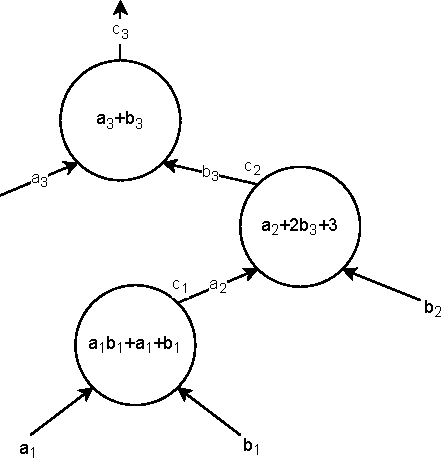
\includegraphics[width=0.4\textwidth]{../figures/plonk-circuit.drawio}
    \caption{Example of a \plonk-like circuit.}
    \label{figure:plonk-circuit-example}
\end{figure}

Observe all the values below depend only on the shape of the circuit itself, so if the circuit does not change, this polynomial should not be recomputed. Check that the \SA, \SB and \SC polynomials are constructed so that we can verify the copy-constraints $c_2 = b_3$ and $c_1 = a_2$ present in the circuit. Observe that equally painted cells have their values swapped, as explained before in the construction of the connection $S$ polynomials.  

\begin{figure}[H]
    \centering
    \begin{tabular}{|c|c|c|c|c|c|c|c|}
        \hline
        \QL	&\QR	&\QM	&\QO	&\QC	&\SA					&\SB						&\SC 							\\ \hline
        1			&1				&1				&-1				&0				&1								&$k_1$								&\cellcolor{pink} $g$				\\
        1			&2				&0				&-1				&3				&\cellcolor{pink}$k_2$			&$k_1 \cdot g$					&\cellcolor{cyan} $k_1 \cdot g^2$	\\
        1			&1				&0				&-1				&0				&$g^2$						&\cellcolor{cyan}$k_2 \cdot g$ &$k_2 \cdot g^2$					\\
        \hline
    \end{tabular}
    \label{table:plonk-circuit-example}
\end{figure}

Therefore, we can derive a PIL program that validates the previous circuit as shown below:
\begin{pil}
    include "config.pil";
    
    namespace Plonk(%N);
    pol constant QL, QR, QM, QO, QC;
    pol constant SA, SB, SC;
    pol constant L1;
    
    pol commit a, b, c;
    
    public pi = a(0);
    
    // Public values check 
    L1 * (a - :pi) = 0;
    
    // Plonk equation 
    pol ab = a*b;
    QL*a + QR*b + QM*ab + QO*c + QC = 0;
    
    // Copy-constraints check 
    {a, b, c} connect {SA, SB, SC};
\end{pil}




%%%%%%%%%%%%%%%%%%%%%%%%%%%%%%%%%%%%%%%%%%%%%%%%%%%%%%%%%%%%%%%%
\subsection{Filling Polynomials}

Until now we have only shown how to specify some kinds of constraints that several polynomials of a certain program described in PIL should satisfy to become \textit{correct}. All these constraints, together with the constant polynomials inherent to the computation itself, specify the transition function underlying the program definition. In other words, changing either any of the constraints or the description of the constant polynomials produces a change in the program we are working on. 

%TODO Check this paragraph
In this section, we are going to use Javascript and \pilcom to generate a specific execution trace for a given PIL. To do so, we are going to compute a valid execution trace for the example of Section \ref{sec:connecting-sm}. As a remark, we will also use the library \texttt{pil-stark} whose utility is to provide a framework to setup, generate and verify proofs, to use a \texttt{FGL} class which mimics a finite field and it is required by some functions that provide the \pilcom package. 

First of all, under the scope of an asynchronous function called \texttt{execute}, we parse the provided PIL (which is, in our case, \texttt{main.pil}) into a Javascript object using the \texttt{compile} function of \pilcom. In code we obtain:
\begin{js}
    const { FGL } = require("pil-stark");
    const { compile } = require("pilcom");
    const path = require("path");
    
    async function execute() {
        const pil = await compile(FGL, path.join(__dirname, "main.pil"));
    }
\end{js}

The \pilcom package also provides two functions that use the \texttt{pil} object to create two crucial objects from it for the construction of the execution trace: the constant polynomials object and the committed polynomials object (using \texttt{newConstPolsArray} and \texttt{newCommitPolsArray} functions, respectively).
\begin{js}
    const { newConstantPolsArray, newCommitPolsArray, compile } = require("pilcom");
    
    async function execute() {
        
        // ... Previous Code
        
        const constPols =  newConstantPolsArray(pil);
        const cmPols = newCommitPolsArray(pil);
    }
\end{js}

Both such objects contain useful information about the PIL itself, such as the provided length of the program $N$, the total number of constant polynomials and the total number of committed polynomials. However, accessing these objects will allow us to fill the entire execution trace for that PIL. We can access a specific position of the execution trace using the syntax:
\begin{js}
    pols.Namespace.Polynomial[i] 
\end{js}
being \texttt{pols} one of the previously introduced \texttt{constPols} and \texttt{cmPols} objects, \texttt{Namespace} being a specific namespace among the ones defined by the PIL files, \texttt{Polynomial} one of the polynomials defined under the scope of the previous namespace and $i$ an integer in the set $[0,N-1]$ representing the row of the current polynomial. Using this we can now start to fill our polynomials. 

In our example, we will use, as inputs for the trace, which are the ones introduced in the \texttt{Main.a} polynomial, an ascending chain of integers from $0$ to $15$ cyclically (because recall that we are only allowed to use $4$ bits integers). We propose here two functions that fill the constant and committed polynomials accordingly. 
\begin{figure}[H]
    \begin{js}
        async function buildConstantPolynomials(constPols, polDeg) {
            
            for (let i=0; i < polDeg; i++) {
                constPols.Global.BITS4[i] = BigInt(i & 0b1111);
                constPols.Global.L1[i] = i === 0 ? 1n : 0n;
                constPols.Negation.RESET[i] = (i % 4) == 3 ? 1n : 0n;
                constPols.Negation.FACTOR[i] = BigInt(1 << (i % 4));
                constPols.Negation.ISLAST[i] = i === polDeg-1 ? 1n : 0n;
            }
        }
    \end{js}
    \caption{Generation of the constant polynomials.}
\end{figure}

\begin{figure}[H]
    \begin{js}
        async function buildcommittedPolynomials(cmPols, polDeg) {
            
            cmPols.Negation.a[-1] = 0n;
            cmPols.Negation.neg_a[-1] = 1n;
            
            for (let i=0; i < polDeg; i++) {
                
                let fourBitsInt = i % 16;
                
                cmPols.Main.a[i] = BigInt(fourBitsInt);
                cmPols.Main.neg_a[i] = BigInt(fourBitsInt ^ 0b1111);
                cmPols.Main.op[i] = FGL.mul(cmPols.Main.a[i], cmPols.Main.neg_a[i]);
                
                cmPols.Multiplier.freeIn1[i] = cmPols.Main.a[i];
                cmPols.Multiplier.freeIn2[i] = cmPols.Main.neg_a[i];
                cmPols.Multiplier.out[i] = cmPols.Main.op[i];
                
                let associatedInt = Math.floor(i/4);
                let bit = (associatedInt >> (i%4) & 1) % 16;
                cmPols.Negation.bits[i] = BigInt(bit);
                cmPols.Negation.nbits[i] = BigInt(bit ^ 1);
                
                
                let factor = BigInt(1 << (i % 4));
                let reset = (i % 4) == 0 ? 1n : 0n;
                cmPols.Negation.a[i] = factor*cmPols.Negation.bits[i] 
                + (1n-reset)*cmPols.Negation.a[i-1];
                cmPols.Negation.neg_a[i] = factor*cmPols.Negation.nbits[i] 
                + (1n-reset)*cmPols.Negation.neg_a[i-1];
            }
        }
    \end{js}
    \caption{Generation of the committed polynomials.}
\end{figure}

Now that we have all the constant and committed polynomials filled in, we can check using a function called \texttt{verifyPil} that they indeed satisfy the constraints defined in the PIL file. We provide below the piece of code that construct the polynomials and check the constraints. If the verification procedure fails, we should not proceed to the proof generation because it will lead to false proof. 
\begin{js}
    const { newConstantPolsArray, newCommitPolsArray, compile, verifyPil } = require("pilcom");
    
    async function execute() {
        
        // ... Previous Code	
        
        const N = constPols.Global.BITS4.length;
        
        await buildConstantPolynomials(constPols, N);
        await buildcommittedPolynomials(cmPols, N);
        
        const res =  await verifyPil(FGL, pil, cmPols , constPols);
        if (res.length != 0) {
            console.log("The execution trace do not satisfy PIL restrictions. Aborting...");
            for (let i=0; i<res.length; i++) {
                console.log(res[i]);
                return;
            }
        }
    }
\end{js}







%TODO: Is this section necessary?
%%%%%%%%%%%%%%%%%%%%%%%%%%%%%%%%%%%%%%%%%%%%%%%%%%%%%%%%%%%%%%%%%
\subsection{Generating a Proof Using \texttt{pil-stark}}

Once the constant and the committed polynomials are filled, we can step to the proof generation stage. We can use the \texttt{pil-stark} Javascript package specially designed to work together with \pilcom to generate STARK proofs about PIL statements. We will use three functions \texttt{starkSetup}, \texttt{starkGen} and \texttt{starkVerify} from the package. The first one is aiming for setting up the STARK, which is independent of the values of committed polynomials. This includes the computation of the tree of the evaluations of the constant polynomials. For executing the setup generation we ought to have an object called \texttt{starkStruct} which is specifying several FRI-related parameters such as the size of the trace domain (which must coincide with $N$, defined in PIL), the size of the extended domain (which together with the previous parameter specifies the correspondent \textit{blowup factor}), the number of queries to be executed and the reduction factors for each of the FRI steps. We execute the setup using the code below:

\begin{js}
    const { FGL, starkSetup } = require("pil-stark");
    
    async function execute() {
        
        // ... Previous Code	
        
        const starkStruct = {
            "nBits": 10,
            "nBitsExt": 11,
            "nQueries": 128,
            "verificationHashType": "GL",
            "steps": [
            {"nBits": 11},
            {"nBits": 5},
            {"nBits": 3},
            {"nBits": 1}
            ]
        };
        
        const setup = await starkSetup(constPols, pil, starkStruct);
    }
\end{js}

Now that we have set up the STARK, we can generate the proof using the \texttt{starkGen} function. We can do this task using the code below. Observe that the \texttt{setup} object contains inside a \texttt{starkInfo} field which contains, aside from all the \texttt{starkStruct} parameters, lots of useful information about the shape of the PIL itself. 

\begin{js}
    const { FGL, starkSetup, starkGen } = require("pil-stark");
    
    async function execute() {
        
        // ... Previous Code	
        
        const resProof = await starkGen(cmPols, constPols, setup.constTree, setup.starkInfo);
    }
\end{js}

Now that a proof has been generated we can be involved in the verification procedure invoking the \texttt{starkVerify} function. This function needs, as arguments, some information provided by the outputs of both the \texttt{starkSetup} and \texttt{starkGen} functions. If the output of the \texttt{starkVerify} function is \texttt{true}, the proof is valid. Otherwise, the verifier should invalidate the proof sent by the prover. 

\begin{js}
    const { FGL, starkSetup, starkGen, starkVerify } = require("pil-stark");
    
    async function execute() {
        
        // ... Previous Code
        
        const resVerify = await starkVerify(
        resP.proof, resP.publics, setup.constRoot, setup.starkInfo
        );
        
        if (resVerify === true) {
            console.log("The proof is VALID!");
        } else {
            console.log("INVALID proof!");
        }
    }
\end{js}


%%%%%%%%%%%%%%%%%%%%%%%%%%%%%%%%%%%%%%%%%%%%%%%%%%%%%%%%%%%%%%% 
\section{zkASM instructions set} \label{sec:instructions}

\subsection{Memory Related Instructions}


We refer to the memory as a volatile read-write data storage that exists only during the execution of a zkASM program. The memory is divided into different contexts of \texttt{0x40000} words. Each word is 256 bits in length, so each context is 8 MB in size.

Each context is divided into the following three blocks:

\begin{itemize}
    
    \item \textbf{VARS:} With a relative offset of \texttt{0x00000} and a height of \texttt{0x10000} words (\texttt{2MB}), contains the local context variables pre-defined in the language. The list of all context variables can be found at \href[]{https://github.com/0xPolygonHermez/zkevm-rom/blob/main/main/vars.zkasm}{\texttt{vars.zkasm}}.
    
    \item \textbf{STACK:} With a relative offset of \texttt{0x10000} and a height of \texttt{0x10000}  words  \texttt{(2MB)}, contains the stack of the the EVM. \textbf{STACK} is defined once per context.
    
    \item \textbf{MEMORY:} With a relative offset of \texttt{0x20000} and a height of \texttt{0x20000} words \texttt{(4MB)}, contains the free memory that can be freely used. \textbf{MEMORY}, like \textbf{STACK}, is also defined once per context. 
\end{itemize}

Therefore, for a given slot in memory, its pointer is computed as:
\[
\texttt{memoryAddress} = \texttt{0x40000} \cdot \texttt{CTX} + \texttt{isStack} \cdot (\texttt{0x10000} + \texttt{SP}) + \texttt{isMem} \cdot (\texttt{0x20000} + \texttt{offset})
\]
where:

\begin{itemize}
    
    \item \texttt{CTX}: This integer variable refers to the memory context being accessed in the EVM's memory. 
    
    \item \texttt{isStack}:  this boolean value indicates whether the memory operation being performed is related to the EVM's stack. The EVM uses a stack-based architecture, meaning that operations are performed by pushing and popping values on and off the stack.
    
    \item \texttt{SP}: This variable refers to the current position of the stack pointer in the EVM's stack. The stack pointer is used to keep track of the current top of the stack. More information on \texttt{SP} will be added below.
    
    \item \texttt{isMem}: This boolean value indicates whether the memory operation being performed is related to the EVM's memory. Observe that \texttt{isStack} and \texttt{isMem} can not be $1$ at the same time. 
    
    \item \texttt{offset}:  This variable likely refers to the offset or location within the current memory context being accessed.
    
\end{itemize}

Observe that, following the above description of the memory, the former set of variables completely determine a memory slot. Figure ?? shows the structure of the memory during a zkASM execution.

\begin{figure}[H]
    \centering
    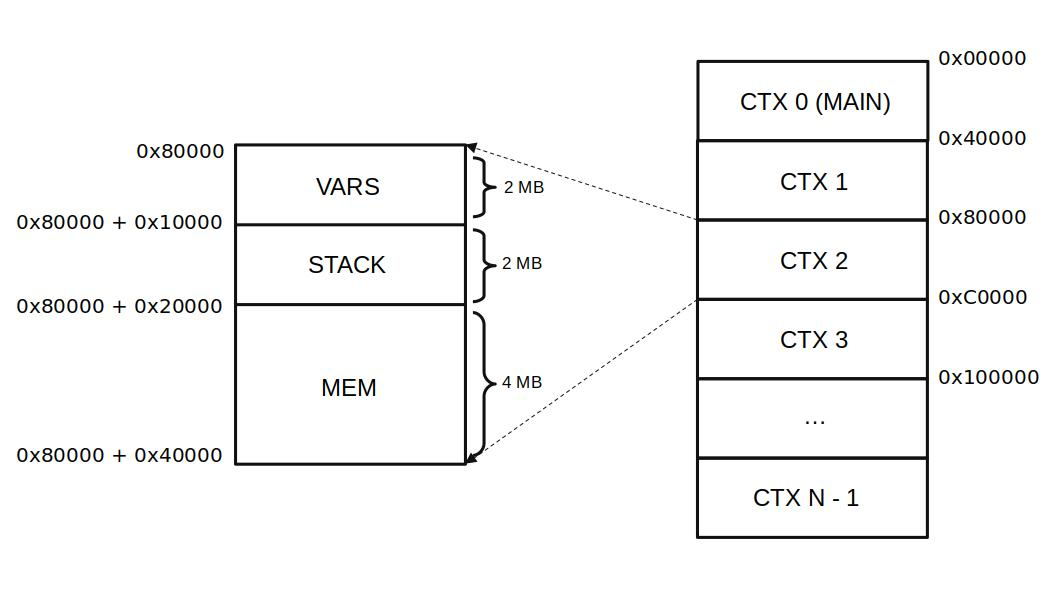
\includegraphics[width=0.6\columnwidth]{\assemblydir/figures/memory-regions}
    \caption{Schema of contexts and memory regions of the zkEVM.}
    \label{fig:memory-regions}
\end{figure}

In order to allow runtime interaction with memory, zkASM has a couple of instructions to read and write values to it.



Let us first define how can be access to a specific address of the memory. Memory acess will be parametrized by $2$ integer parameters: the address \addr and the relative address \relAddr. 

\begin{itemize}

\item \addr: Address would be able to define a memory access up to memory region level. That is, \addr will contain information of which context access the memory and if the access is directed to the system variables \textbf{VARS}, the \textbf{STACK} or the \textbf{MEMORY}.

\item \relAddr: However, \addr is not enough. Hence, \relAddr will point to a specific memory slot inside a concrete memory region of a context. We should take into account that \relAddr can never be negative. Moreover, \relAddr is also bounded from above: if we are accessing to the \textbf{MEMORY}, \relAddr should be strictly less than \texttt{0x40000} (because memory measures $\texttt{4MB}$) and if we are accessing to the \textbf{STACK} or to the system variables \textbf{VARS}, \relAddr should be strictly less than \texttt{0x10000} (because both memory regions measure $\texttt{2MB}$). Then, the wanted memory slot will be equal to $\addr + \relAddr$.

\end{itemize}

Let us know how to specify \addr and \relAddr in zkASM language. We can specify \addr with $3$ keywords: \texttt{SYS} (which corresponds to \textbf{VARS} memory region), \texttt{STACK} (which corresponds to \textbf{STACK} memory region) and \texttt{MEM} (which corresponds to \textbf{MEMORY} memory region). Invoking \texttt{STACK} will increase \addr by $\texttt{0x10000}$ and similarly, invoking \texttt{MEM} will increase \addr by \texttt{0x20000}. However, since \textbf{VARS} is the first memory region, it will not produce an increase in \addr. Moreover, \addr will also increase depending on the current context. More specifically, a total amount of \texttt{0x40000} will be increased per context, following our memory description above. 

To specify \relAddr we can use $2$ registers: \E and \RR. If \E is chosen, \relAddr will increase a total amount of $\E_0$ units. Similarly, if \RR is chosen, \relAddr will increase by \RR. Moreover, we can add a numeric offset to increase a fixed amount of units \addr + \relAddr. 

The syntax will be, in each case:

\begin{zkasm}
addr:relAddr 
; or
addr:relAddr+offset
; or 
addr:relAddr-offset
\end{zkasm}

Below, we specify concrete examples on how to specify addresses:

\begin{zkasm}
SYS:E
SYS:E+1
STACK:RR
MEM:E 
MEM:E-2
MEM:RR+1
\end{zkasm}

To end up, we can also access to addresses by means of global and local variables, defined elsewhere in the assembly code. This variables will have a unique identifier that we will use in order to access to it.


\subsubsection{\MLOAD}


\MLOAD is the zkASM instruction used to read a value from a specific address in memory. It takes the pointer address of the memory slot to be read as a parameter. We can store the value that is read in a register of our choosing by using the free input (\texttt{\$}) assignment. 

Suppose that we want to read the memory value stored in the address \texttt{someAddr} in a certain context. The address \texttt{someAddr} is defined by the global variable:
\begin{zkasm}
VAR GLOBAL someAddr
\end{zkasm}

The following zkASM code stores the corresponding value into the register \A:
\begin{zkasm}
$ => A          :MLOAD(someAddr)
\end{zkasm}





\subsubsection{\MSTORE}


\MSTORE is the zkASM instruction used to write a value to a specific address in memory. It takes the pointer address of the memory slot to be read as a parameter, the register that contains the value to be writed must be also specified.

The following example shows how to store in the memory the value of the current context. Note that as the \MSTORE parameter, it is specified the variable that contains the pointer to where current context is stored in the memory. The value stored will be taken from \texttt{CTX} register:
\begin{zkasm}
CTX       :MSTORE(currentCTX)      
\end{zkasm}



\subsubsection{Dealing with the STACK}

A stack machine is a machine in which temporary values for computations are moved to and from a push down stack. Operations over the stack are the typical: \texttt{PUSH}, \texttt{POP}, \texttt{DUP}, \texttt{SWAP}, etc. Since the EVM is a stack-based virtual machine, we reserve an address space to create a stack within the memory of the zkEVM. The classical pointer called \texttt{STACK POINTER} (\texttt{SP}) contains the address of the \textbf{next free position on the} \texttt{STACK}. A \texttt{POP} from the \texttt{STACK} can be implemented as:

\begin{zkasm}
SP -1 => SP
$ => A		:MLOAD(SP)
\end{zkasm}

where we decrement \texttt{SP} to reposition it on the last element of the stack and
then we load this element into registry \A. Similarly, a \texttt{PUSH} into the \texttt{STACK} can be implemented as:

\begin{zkasm}
0		:MSTORE (SP++)
\end{zkasm}

which saves a \texttt{0} at the top of the stack and increments \texttt{SP}. An important note about both the stack and the memory is that the stack pointer and the memory are per context.




\subsubsection{\MEMALIGNRD}

Although the memory word in zkASM is 256 bits long, in roder to mimic the regular Ethereum Virtual Machine (EVM) memory behavior, zkASM has a specific instructions for accessing memory at the byte level. The instruction \MEMALIGNRD enables reading 32 bytes starting from an offset of any byte in memory. In this way, two memory registers are read and a the following transformation is applied to virtually obtain a new 32-byte word as a result of the reading.
\begin{align*}
    \texttt{val} &= \Bigr[ \texttt{m}_0 \ll 8 \cdot \texttt{offset} \Bigr] \mathbin\Vert \Bigr[ \texttt{m}_1 \gg 256- 8 \cdot \texttt{offset} \Bigr] 
\end{align*}

Here, the symbol $\mathbin\Vert$ denotes string concatenation. The registers must be set as follows before call the \MEMALIGNRD instruction. We can store the value that is read in a register of our choosing by using the free input (\texttt{\$}) assignment.


\begin{figure}[h!]
    \renewcommand{\figurename}{Table}
    \[
    \begin{array}{|c|c|}
        \hline
        \mathbf{Register} &\mathtt{MEM\_ALIGN\_RD} \ \mathbf{parameters} \\ \hline
        \A & \texttt{Memory Slot of } \mathtt{m_0} \\
        \B & \texttt{Memory Slot of } \mathtt{m_1} \\
        \C & \texttt{offset} \\
        \hline
    \end{array}
    \]
    \caption{\MEMALIGNRD instruction parameters.}
    \label{tab:memory-first-example}
\end{figure}

The following example shows how to read 32 bytes that are stored occupying part of two consecutive zkASM memory words. The read value will be stored in register \A:

\begin{zkasm}
$ => A          :MLOAD(someAddr)
$ => B          :MLOAD(someAddr+1)
16 => C

$ => A          :MEM_ALIGN_RD
\end{zkasm}

Figure ?? shows how the 32-bytes value will be read for the \MEMALIGNRD given example.

\begin{figure}[H]
    \centering
    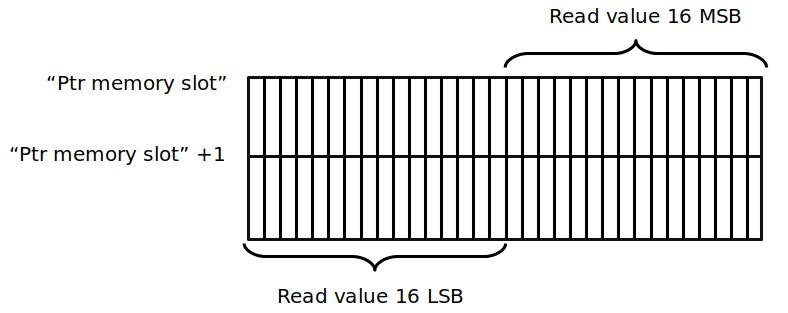
\includegraphics[width=0.8\columnwidth]{\assemblydir/figures/mem-align-wr}
    \caption{Example of how values are read from the memmory using \MEMALIGNRD with an offset of 16.}
    \label{fig:memory-regions}
\end{figure}

\subsubsection{\MEMALIGNWR}
\MEMALIGNWR is equivalent to \MEMALIGNRD but for writing a 32-byte value. In this case, we have to specify two memory slots that will be written after applying the following transformation to the value to be stored. The registers that contains the value to be stored must also be specified.
\begin{align*}
    \texttt{w}_0 &= \Bigr[ \texttt{m}_0 \ \texttt{\&} \ \left(2^{256} - 2^{256-8 \cdot \texttt{offset}} \right) \Bigr] \mathbin\Vert \Bigr[  \texttt{val} \ll 8 \cdot \texttt{offset} \Bigr]  \\
    \texttt{w}_1 &= \Bigr[ \texttt{m}_1 \ \texttt{\&} \ \left( \left( 2^{256} - 1\right)  \gg 8 \cdot \texttt{offset}\right) \Bigr] \mathbin\Vert \Bigr[ \texttt{val} \ll 8 \cdot \texttt{offset} \Bigr] 
\end{align*}

\begin{figure}[h!]
    \renewcommand{\figurename}{Table}
    \[
    \begin{array}{|c|c|}
        \hline
        \mathbf{Register} &\mathtt{MEM\_ALIGN\_WR} \ \mathbf{parameters} \\ \hline
        \A & \texttt{Memory Slot of } \mathtt{m_0}  \\
        \B & \texttt{Memory Slot of } \mathtt{m_1}  \\
        \C & \mathtt{offset} \\
        \D & \mathtt{w_0} \\
        \E & \mathtt{w_1} \\
        \op& \texttt{Value to be written} \\
        \hline
    \end{array}
    \]
    \caption{\MEMALIGNWR instruction parameters.}
    \label{tab:memory-first-example}
\end{figure}

The following example shows how to write 32 bytes that are stored occupying part of two consecutive zkASM memory words. The value to be stored will be taken from free input register:

\begin{zkasm}
$ => A          :MLOAD(MEM:E)
$ => B          :MLOAD(MEM:E+1)

${memAlignWR_W0(A,mem.bytesToStore,C)} => D                    ; no trust calculate W0
${memAlignWR_W1(B,mem.bytesToStore,C)} => E                    ; no trust calculate W1
$               :MEM_ALIGN_WR,MLOAD(bytesToStore)
\end{zkasm}

\subsubsection{\MEMALIGNWRE}

\MEMALIGNWRE allows writing only 8 bits of a specific memory slot. In this case, we have to specify the memory slot to be written, the register that contains the byte to be stored, and the offset value that situates the byte in a specific position of the 32-byte word. The value will be written after applying the following transformation:
\begin{align*}
    \texttt{w}_0 &= \Bigr[ \texttt{m}_0 \ \texttt{\&} \ \left( \texttt{maskByte} \gg 8 \cdot \texttt{offset} \right) \Bigr]  \mathbin\Vert \Bigr[ \left( \texttt{bits} \ \texttt{\&} \ \texttt{0xFF} \right)  \ll 8 \cdot \left( 31-\texttt{offset}\right) \Bigr] 
\end{align*}
where $\texttt{maskByte}$ equals $2^{256} - 1$. 

\begin{figure}[h!]
    \renewcommand{\figurename}{Table}
    \[
    \begin{array}{|c|c|}
        \hline
        \mathbf{Register} &\mathtt{MEM\_ALIGN\_WR8} \ \textbf{parameters} \\ \hline
        \A & \texttt{Memory Slot of } \mathtt{m_0} \\
        \C & \mathtt{offset} \\
        \D & \mathtt{w_0} \\
        \op& \texttt{Value to be written} \\
        \hline
    \end{array}
    \]
    \caption{\MEMALIGNWRE instruction parameters.}
    \label{tab:memory-first-example}
\end{figure}

The following example shows how to write $1$ bytes stored in the byte $4$ of a specific storage slot. The value to be stored will be taken from \B register:

\begin{zkasm}
4 => C
$ => A          :MLOAD(someAddr)
${memAlignWR8_W0(A,B,C)} => D  ; no trust calculate W0
B               :MEM_ALIGN_WR8 ; only use LSB of B, rest of bytes could be non zero
\end{zkasm}

\subsection{Storage Related Instructions}

Polygon zkEVM, like Ethereum L1, has a storage component for storing persistent on-chain data, which includes the balances of all accounts, their nonces, and the state of all deployed smart contracts along with their codes. The data that forms the state is represented as cryptographic trie, but while Ethereum L1 uses a modified Patricia tree with Keccak256 as the hash operation, Polygon zkEVM uses a binary sparse Merkle tree with Poseidon as the hash operation (refer to the technical documents regarding the zkEVM bridge annex A to learn more about sparse Merkle trees).

Poseidon is a hash function that's specifically designed for use in zero-knowledge applications, as it's meant to operate with values of a prime field and it has been proven to be much more performant than Keccak256 in zero-knowledge constructions like those used in Polygon zkEVM. Moreover Poseidon hash has an input named capacity, which can be used as an extra input value.

Barely, the Polygon zkEVM state tree is a key-value structure in which the integrity can be ensured by a 256-bit value known as the state root. Each entry in the tree is a leaf and directly stores a 256-bit value. Additionally, the index position of that leaf in the tree corresponds to the 256-bits of the key. As can be seen in Figure X, since the keys are 256-bits in length, the tree has 32 levels and a total capacity of $2^{256}$ leaves.


\begin{figure}[H]
    \centering
    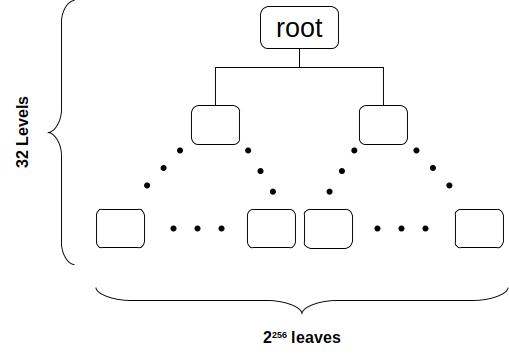
\includegraphics[width=0.6\columnwidth]{\assemblydir/figures/state-trie}
    \caption{Polygon zkEVM state trie.}
    \label{fig:hashk-add-bytes}
\end{figure}

Since five different types of values can be stored, a distinction must be made among the five types of leaves. Table X shows the relation between leaf type and the corresponding data types that they contain.

\begin{figure}[h!]
    \renewcommand{\figurename}{Table}
    \[
    \begin{array}{|c|c|}
        \hline
        \mathbf{Leaf~type} &\mathbf{Data~type} \\ \hline
        \mathtt{0} & \mathtt{Account~balance} \\
        \mathtt{1} & \mathtt{Account~nonce} \\
        \mathtt{2} & \mathtt{Contract~code~hash} \\
        \mathtt{3} & \mathtt{Contract~storage~slot~value} \\
        \mathtt{4} & \mathtt{Contract~code~length} \\
        \hline
    \end{array}
    \]
    \caption{Polygon zkEVM state tree leaf types.}
    \label{tab:memory-first-example}
\end{figure}


For each leaf entered in the tree its key is computed as follows:

$$\texttt{key} = \texttt{Poseidon}(\texttt{key\_seed})$$

where \texttt{key\_seed} is a $32$-bytes integer constructed as follows:
\[
\texttt{key\_seed} = (\texttt{account\_address} \mid\mid \texttt{0x00000000} \mid\mid \texttt{leaf\_type} \mid\mid \texttt{0x00000000})
\]
being $\texttt{account\_address} \in \{0, 1, \dots, 2^{160} - 1\}$ is a $20$-bytes integer and $\texttt{leaf\_type} \in \{0, 1, \dots, 2^{32} - 1\}$ a $4$-bytes integer.

The capacity of the Poseidon's instance used when computing keys is always zero except in the case where the leaf corresponds to a contract storage slot value (leaf type 3), in which case the capacity is directly set to the storage slot pointer. It's important to note that because the contract storage slot pointer is not encoded in the 32-byte input, if we do not use the capacity, all storage slots for the same contract would lead to the same state tree leaf.

Te value sored in the leaf has the following structure:
\[
(v_0, \dots, v_7)
\]
codifying a $256$-bits unsigned integer, where $v_i \in \FF_p$ are bounded to $32$-bits each. 

In order to allow runtime interaction with the Polygon zkEVM state tree zkASM has a couple of instructions to read and write values on it.

\subsubsection{\texttt{SLOAD}}

\texttt{SLOAD} is the zkASM instruction used to read a value from a leaf in the state tree. It takes Poseidon's ``Input" and ``Capacity" parameters, along with the leaf type, to compute the key of the leaf to be read. The registers must be set as follows before call the \texttt{SLOAD} instruction.

\begin{figure}[h!]
    \renewcommand{\figurename}{Table}
    \[
    \begin{array}{|c|c|}
        \hline
        \mathbf{Register} &\texttt{SLOAD } \textbf{parameters} \\ \hline
        \A & \mathtt{Account~address} \\
        \B & \mathtt{Leaf~type} \\
        \C & \mathtt{Contract~storage~slot~pointer~(capacity)} \\
        \hline
    \end{array}
    \]
    \caption{\texttt{SLOAD} instruction parameters.}
    \label{tab:memory-first-example}
\end{figure}

We can store the value that is read in a register of our choosing by using the free input (\texttt{\$}) assignment.

The following example shows how to read the balance of a specific account, the value that is read will be stored in the \E register:

\begin{zkasm}
someAccountAddr => A          
0 => B      
0 => C          
$ => E          :SLOAD
\end{zkasm}

The following example shows how to read a storage slot of a specific contract, the value that is read will be stored in the \E register:

\begin{zkasm}
someAccountAddr => A          
3 => B      
storageSlotPtr => C 
$ => E          :SLOAD
\end{zkasm}

\subsubsection{\texttt{SSTORE}}

\texttt{SSTORE} is the zkASM instruction used to store a value to a leaf in the state tree. It takes Poseidon's ``Input" and ``Capacity" parameters, along with the leaf type, to compute the key of the leaf to be writen, in addition takes the value to be written. The registers must be set as follows before call the \texttt{SSTORE} instruction.

\begin{figure}[h!]
    \renewcommand{\figurename}{Table}
    \[
    \begin{array}{|c|c|}
        \hline
        \mathbf{Register} &\texttt{SSTORE } \textbf{parameters} \\ \hline
        \A & \mathtt{Account~address} \\
        \B & \mathtt{Leaf~type} \\
        \C & \mathtt{Contract~storage~slot~pointer~(capacity)} \\
        \D & \mathtt{Value~to~write} \\
        \hline
    \end{array}
    \]
    \caption{\texttt{SSTORE} instruction parameters.}
    \label{tab:memory-first-example}
\end{figure}

The following example shows how to write a storage slot of a specific contract:

\begin{zkasm}
someAccountAddr => A          
3 => B      
storageSlotPtr => C          
value => D         
A               :SSTORE
\end{zkasm}




%%%%%%%%%%%%%%%%%%%%%%%%%%%%%%%%%%%%%%%%%%%%%%%%%%%%%%%%%%%%%%%

\subsection{Binary-Related Instructions}

The arithmetic operators are used to perform arithmetic mathematical operations on numeric data stored in registers.

\subsubsection{\ADD}

\ADD is used to sum the content of the registers \A and \B, the result will be treated as a free input. The following example shows how to use \ADD instruction.

\begin{zkasm}
val1 => A          
val2 => B          

$ => C             :ADD ; [ val1 + val2 => C]
\end{zkasm}

\subsubsection{\SUB}

\SUB is used to subtract de content fo register \B to \A, the result will be treated as a free input. The following example shows how to use \SUB instruction.

\begin{zkasm}
val1 => A          
val2 => B          

$ => C             :SUB ; [ val1 - val2 => C]
\end{zkasm}



\subsubsection{\LT}

\LT instruction is used to compare the values of the registers \A and \B as \textbf{unsigned integers}. The output of the operation will be $1$ if \A is actually lower than \B (that is, $\A < \B$) and $0$ otherwise (that is, $\A \geq \B$). The output of the instruction will be treated as a free input. The next lines of code show an example on how to use \LT instruction:

\begin{zkasm}
valA => A
valB => B

$ => C			:LT ; [1 if A < B, 0 if A <= B]
\end{zkasm}





\subsubsection{\SLT}

\SLT instruction is used to compare the values of the registers \A and \B as \textbf{signed integers}, explained in Section \ref{sec:binary-sm}. The output of the operation will be $1$ if \A is actually lower than \B (that is, $\A < \B$) and $0$ otherwise (that is, $\A \geq \B$). The output of the instruction will be treated as a free input. The next lines of code show an example on how to use \SLT instruction:

\begin{zkasm}
valA => A
valB => B

$ => C			:SLT ; [1 if A < B, 0 if A <= B]
\end{zkasm}


\subsubsection{\EQ}

\EQ instruction is used to compare the equality relationship between the values of the registers \A and \B. The output of the operation will be $1$ if \A is equal to \B (that is, $\A = \B$) and $0$ otherwise (that is, $\A \neq \B$). The output of the instruction will be treated as a free input. The next lines of code show an example on how to use \EQ instruction:

\begin{zkasm}
valA => A
valB => B

$ => C			:EQ ; [1 if A = B, 0 if A != B]
\end{zkasm}


\subsubsection{\AND}


\AND instruction is used to perform the bit-wise \AND operation between registers \A and \B, as explained in Section \ref{sec:binary-sm}. The output of the instruction will be treated as a free input. The next lines of code show an example on how to use \AND instruction:

\begin{zkasm}
valA => A
valB => B

$ => C			:AND
\end{zkasm}

For sake of completeness, let us propose a more concrete example, where we assign the value $\texttt{0xDBn}$ to \A and the value $\texttt{0x86n}$ to \B. The result of the bit-wise \AND operation is going to be \texttt{0x82n} because
\[
\A = \texttt{0b11011011}, \quad \B = \texttt{0b10000110} \Longrightarrow \C = \texttt{0b10000010}.
\]

\begin{zkasm}
0xDBn => A
0x86n => B

$ => C			:AND ; C = 0x82n
\end{zkasm}

\subsubsection{\OR}

\OR instruction is used to perform the bit-wise \OR operation between registers \A and \B, as explained in Section \ref{sec:binary-sm}. The output of the instruction will be treated as a free input. The next lines of code show an example on how to use \OR instruction:

\begin{zkasm}
valA => A
valB => B

$ => C			:OR
\end{zkasm}

For sake of completeness, let us propose a more concrete example, where we assign the value $\texttt{0xDBn}$ to \A and the value $\texttt{0x86n}$ to \B. The result of the bit-wise \OR operation is going to be \texttt{0xDFn} because
\[
\A = \texttt{0b11011011}, \quad \B = \texttt{0b10000110} \Longrightarrow \C = \texttt{0b11011111}.
\]

\begin{zkasm}
0xDBn => A
0x86n => B

$ => C			:OR ; C = 0xDFn
\end{zkasm}



\subsubsection{\XOR}

\XOR instruction is used to perform the bit-wise \XOR operation between registers \A and \B, as explained in Section \ref{sec:binary-sm}. The output of the instruction will be treated as a free input. The next lines of code show an example on how to use \XOR instruction:

\begin{zkasm}
valA => A
valB => B

$ => C			:XOR
\end{zkasm}

For sake of completeness, let us propose a more concrete example, where we assign the value $\texttt{0xDBn}$ to \A and the value $\texttt{0x86n}$ to \B. The result of the bit-wise \XOR operation is going to be \texttt{0x5Dn} because
\[
\A = \texttt{0b11011011}, \quad \B = \texttt{0b10000110} \Longrightarrow \C = \texttt{0b01011101}.
\]

\begin{zkasm}
0xDBn => A
0x86n => B

$ => C			:XOR ; C = 0x5Dn
\end{zkasm}





%%%%%%%%%%%%%%%%%%%%%%%%%%%%%%%%%%%%%%%%%%%%%%%%%%%%%%%%%%%%%%%
\subsection{Arithmetic-Related Instructions}

\subsubsection{\ARITH}

The \ARITH instruction allows to check field operations. More specifically, it checks a combination of an addition and a product, as explained in Section \ref{sec:arith-sm}. Before calling the \ARITH instruction, registers \A, \B, and \C must be set. The equation that follows will be evaluated using the values of these $3$ registers. It is necessary to specify where the result of the evaluation will be stored. If the evaluation results in an overflow of the output register, the overflow value will be stored in register \D. More specifically, the equation that checks the \ARITH instruction is the following one:

\[
\D \cdot 2^{256} + \op = \A \cdot \B + \C
\]

The following example shows how to use \ARITH instruction. The result of the evaluation will be stored in register \A, and if there is an overflow, it will be stored in register \D:
\begin{zkasm}
valA => A          
valB => B          
valC => C
A            :ARITH ; [ valA * valB + valC => [D,A]]
\end{zkasm}





\subsubsection{\ARITHADDDIFF}

The \ARITHADDDIFF instruction allows to perform additions $P + Q$ over the elliptic curve defined in Section \ref{sec:arith-sm}. This instruction can not perform doublings, since the input points to be added are supposed to be different. This is not explicitly check, but since the doubling formula differs a lot from the distinct point addition formula, the result will be wrong if $P = Q$. The input parameters of the instruction are specified in the table below:

\begin{figure}[h!]
    \renewcommand{\figurename}{Table}
    \[
    \begin{array}{|c|c|}
        \hline
        \mathbf{Register} &\texttt{ARITH\_ECADD\_DIFFERENT } \textbf{parameters} \\ \hline
        \A & x_1, \mathtt{~x~coordinate~of~}P \\
        \B & y_1, \mathtt{~y~coordinate~of~}P \\
        \C & x_2, \mathtt{~x~coordinate~of~}Q \\
        \D & y_2, \mathtt{~y~coordinate~of~}Q \\
        \E & x_3, \mathtt{~x~coordinate~of~}P+Q \\
        \op & y_3, \mathtt{~y~coordinate~of~}P+Q \\
        \hline
    \end{array}
    \]
    \caption{\ARITHADDDIFF instruction parameters.}
    \label{tab:memory-first-example}
\end{figure}

An example on how to use the \ARITHADDDIFF instruction can be seen in the code blow. Observe that we make use of the executor implemented functions \texttt{xAddPointEc(A,B,C,D)} and \texttt{yAddPointEc(A,B,C,D)} which compute the $x$ and the $y$ coordinate of $P + Q$ being $P = (A, B)$ and $Q = (C, D)$ whenever $P \neq Q$. After this is computed, the $x$ coordinate of $P + Q$ is is stored into the memory slot given by the address \texttt{addX} and, similarly, the $y$ coordinate of $P + Q$ is pushed into the memory slot given by the address \texttt{addY}. If we have used incorrect values for the coordinates of $P + Q$, an executor error will pop. This will also be captured when the proof of the batch is generated, since the instruction invocation fills the polynomials of the Arithmetic State Machine correctly. 

\begin{zkasm}
$ => A  						:MLOAD(Px)
$ => B  						:MLOAD(Py)
$ => C  						:MLOAD(Qx)
$ => D  						:MLOAD(Qy)
${xAddPointEc(A,B,C,D)} => E  	:MSTORE(addX)
${yAddPointEc(A,B,C,D)} 		:ARITH_ECADD_DIFFERENT, MSTORE(addY)
\end{zkasm}


\subsubsection{\ARITHADDSAME}

The \ARITHADDSAME instruction allows to perform point doublings $2P$ over the elliptic curve defined in Section \ref{sec:arith-sm}. The input parameters of the instruction are specified in the table below:

\begin{figure}[h!]
    \renewcommand{\figurename}{Table}
    \[
    \begin{array}{|c|c|}
        \hline
        \mathbf{Register} &\texttt{ARITH\_ECADD\_DIFFERENT } \textbf{parameters} \\ \hline
        \A & x_1, \mathtt{~x~coordinate~of~}P \\
        \B & y_1, \mathtt{~y~coordinate~of~}P \\
        \E & x_3, \mathtt{~x~coordinate~of~}2P \\
        \op & y_3, \mathtt{~y~coordinate~of~}2P \\
        \hline
    \end{array}
    \]
    \caption{\ARITHADDDIFF instruction parameters.}
    \label{tab:memory-first-example}
\end{figure}

An example on how to use the \ARITHADDSAME instruction can be seen in the code blow. Observe that we make use of the executor implemented functions \texttt{xDblPointEc(A,B)} and \texttt{yDblPointEc(A,B)} which compute the $x$ and the $y$ coordinate of $2P$ being $P = (A, B)$. After this is computed, the $x$ coordinate of $2P$ is is stored into the memory slot given by the address \texttt{doublePx} and, similarly, the $y$ coordinate of $2P$ is pushed into the memory slot given by the address \texttt{doublePy}. If we have used incorrect values for the coordinates of $2P$, an executor error will pop. This will also be captured when the proof of the batch is generated, since the instruction invocation fills the polynomials of the Arithmetic State Machine correctly. 

\begin{zkasm}
$ => A  					:MLOAD(Px)
$ => B  					:MLOAD(Py)

${xDblPointEc(A,B)} => E  	:MSTORE(doublePx)
${yDblPointEc(A,B)} 		:ARITH_ECADD_SAME, MSTORE(doublePy)
\end{zkasm}









%%%%%%%%%%%%%%%%%%%%%%%%%%%%%%%%%%%%%%%%%%%%%%%%%%%%%%%%%%%%%%%
\subsection{Execution Control Flow Related Instructions}

In order to allow to conditional branch execution of the zkASM programs, 4 different instruction has been included in zkASM instructios set.

\subsubsection{\JMP} % Jump
\JMP is an unconditional jump instruction that always causes a jump in the program's execution flow, regardless of any conditions. It takes an address of the ROM as a parameter to continue the execution flow. To avoid using numeric pointers for jumps, zkASM allows jump destinations to be aliased with custom names. The compiler resolves these aliases and substitutes them with pointers later on.

The following code shows the general usage of \JMP instruction:

\begin{zkasm}
    
; ...
; Executed Code
; ...

        :JMP(destinationLabel)

; ... 
; Non Executed Code
; ... 

destinationLabel:

; ...
; Executed Code
; ...
    
\end{zkasm}

Moreover, we can also parametrize the destination of a jump-like instruction using either the first limb of the register $\E_0$ or the register \RR, using the syntax below:

\begin{zkasm}
        :JMP(RR)
        :JMP(E)
\end{zkasm}

For example, the code below will produce a jump of $5$ units in the execution flow:

\begin{zkasm}
5 => E
            :JMP(E)          
\end{zkasm}

The former syntax will be also available for all the other kind of jumps specified in below sections, including the ones having an else clause.

\subsubsection{\JMPN} % Jump if Negative

\JMPN is a conditional jump instruction that causes a jump in the program's execution flow if a specified register contains a negative number. It takes the address of the ROM as a parameter to continue the execution flow. The register that contains the value to be evaluated must also be specified.

In the following example, the execution flow will be redirected to \texttt{stackUnderflow} in the case that the evaluation of $\SP - 2$ leads to a negative number.

\begin{zkasm}
; check stack underflow
SP - 2          :JMPN(stackUnderflow)
\end{zkasm}

Conditional jumps can also receive an else-clause label. The synatx is very similar:

\begin{zkasm}
A					:JMPN(ifClauseLabel, elseClauseLabel)


ifClauseLabel:
        ; do something
        
        
elseClauseLabel:
        ; do something different
\end{zkasm}

If the value stored in the \A register is negative, then the execution of the program will continue under the \texttt{ifClauseLabel} label. However, if the value of \A is bigger or equal than $0$, then the execution will continue from the label \texttt{elseClauseLabel}. 




\subsubsection{\JMPC} % Conditional jump, if a condition is fullfiled

\JMPC is a conditional jump instruction that causes a jump in the program's execution flow if a specified condition is evaluated  as true. It is used along with the following comparative instructions.
\begin{itemize}
    \item \EQ: Evaluates if register \A value is equal to register \B value.
    \item \LT: Evaluates if register \A value is less than register \B value.
    \item \SLT: Evaluates if register \A value is less than register \B value also comparing negative values.
\end{itemize}

In the following example, the execution flow will be redirected to \texttt{absIsNeg} in the case that the value contained in register \A (namely \val) is a negative number.

\begin{zkasm}
val => A
0 => B
$          :SLT, JMPC(absIsNeg)
\end{zkasm}





\subsubsection{\JMPZ} % Jump if Zero

\JMPZ is a conditional jump instruction that causes a jump in the program's exectuion flow if a specified register contains a 0. In the following example, the execution flow will be redirected to \texttt{readCode} in the case that the value contained in register \A (namely \val) is $0$.

\begin{zkasm}
val => A
A                   :JMPZ(readCode)
\end{zkasm}






\subsubsection{\JMPNC and \JMPNZ}

In addition to all the previously defined execution jumps, there are two more jumps: \JMPNC and \JMPNZ. This kind of jumps works the other way around \JMPC and \JMPZ does. More concretely, in the code below, the execution will jump to the label \texttt{someLabel} if and only if the value stored in the register \A \textbf{is not} zero. Otherwise, if the condition is satisfied, the execution will proceed normally.
\begin{zkasm}

A			:JMPNZ(someLabel)


someLabel:
    ; do something
\end{zkasm}

Hence, the first argument appearing in the instruction denotes now the else-clause. In fact, we can also adopt an if-else structure in this kind of negated instructions:

\begin{zkasm}

A			:JMPNZ(elseLabel, ifLabel)

elseLabel:
    ; do something
    
ifLabel:
    ; do something
\end{zkasm}

In the above piece of code, if the value of \A is not zero, then the execution will jump to the label \texttt{elseLabel} and, otherwise, it will jump to \texttt{ifLabel}. 



\subsubsection{\ASSERT}
\ASSERT is used to ensure that a given register has the same value as register \A. A failing assertion, meaning that the values are unequal, will stop execution and throw error during runtime. Additionally, an execution that contains a failing assertion cannot generate a valid CI proof.

The following code will compare $\val_1$ with $\val_2$, and if they are not equal the execution will be immediately stopped:

\begin{zkasm}
val1 => A
val2 => B
B    		:ASSERT
\end{zkasm}


\subsubsection{Subroutines (\CALL and \RETURN)}


Subroutines allow breaking down the code into smaller sections that can be called by using only a \CALL instruction. A subroutine is designed to be reusable and can be called by other parts of the program. The code of a subroutine always ends with a \RETURN instruction. When a subroutine is called, control is transferred from the main program to the subroutine. The subroutine then executes its code and, when it's finished, control is returned to the point in the main program immediately following the point where the subroutine was called.

An example of subroutine can be the \texttt{ecrecover\_tx} subrutine used in the zkEVM ROM, it is used to recover the signer of a specific ethereum transaction. zkASM code of \texttt{ecrecover\_tx } subrutine can be found \href[]{https://github.com/0xPolygonHermez/zkevm-rom/blob/b27579b89a95a344d09656490a50df5fc67c8417/main/ecrecover/ecrecover.zkasm}{here}.

The following zkASM code shows how to use the \texttt{ecrecover\_tx} subroutine. Once the subroutine is executed, the code will continue on the following line and the recovered address will be in register \A:
\begin{zkasm}
0xd9eba16ed0ecae432b71fe008c98cc872bb4cc214d3220a36f365326cf807d68n => A ; Tx hash
0xddd0a7290af9526056b4e35a077b9a11b513aa0028ec6c9880948544508f3c63n => B ; r
0x265e99e47ad31bb2cab9646c504576b3abc6939a1710afc08cbf3034d73214b8n => C ; s
0x1cn => D ; v
                        :CALL(ecrecover_tx)
\end{zkasm}




\subsubsection{References}

The jump-like instructions we presented earlier provide programmers with the ability to modify the execution flow by jumping to various parts of the code. Similarly, subroutines enable the invocation of other code segments located in different files, allowing for a return to the point of invocation to continue with the original flow. However, what if a programmer wants to jump to a label in a different \texttt{.zkasm} file without returning to the original code? This is where \textbf{References} come in handy.

\textbf{References} allow programmers to combine jump-like instructions with subroutines, which in turn allows for the jumping to a label in another \texttt{.zkasm} file without the need to return to the original code. This results in greater flexibility and modularity in code organization and execution.

To use references, the syntax is as follows:

\begin{zkasm}
:JMP(@someLabel + RR)
\end{zkasm}

Here, \texttt{someLabel} refers to a label located in another \texttt{.zkasm} file. The instruction above jumps to the line of code that corresponds to the value stored in the register \RR under the \texttt{someLabel} label. Additionally, it is possible to parameterize the specific line of code to jump to by adding the value of the first limb of the register $\E_0$ to the reference, as shown below:

\begin{zkasm}
    :JMP(@someLabel + E)
\end{zkasm}

References can also be used for other types of jumps, including conditional jumps with an else condition. For example:

\begin{zkasm}
    :JMPN(@someLabel + RR)
    :JMPZ(@someLabel + E)
    :JMPC(@someLabel + RR, elseLabel)
    ; ...
\end{zkasm}

Moreover, \textbf{References} are also useful even if the tag we are pointing is actually inside the same \texttt{.zkasm} file. This is because, as we have seen before, we can parametrize how many lines we ought to jump \textbf{after} some label using the registers \E and \RR, which we can not using only tag identifiers. 

\subsubsection{\REPEAT}

Although jumps are enough in order to build program loops, a \REPEAT instruction has been introduced in order to easily repeat a certain line of code. The \REPEAT instruction makes use of the \RCX register in order to parametrize the number of times the code should be repeated. To illustrate how to use the \REPEAT instruction, we are going to propose an example:

\begin{zkasm}
10 => A
14 => RCX
A + 2 => A  :REPEAT(RCX)

40  		:ASSERT 
\end{zkasm}

The previous code assigns $10$ to the \A register and $14$ to the repeat counter \RCX. After that, invokes an addition by two units of the \A register, together with the \REPEAT instruction with parameter \RCX. This will make the line of code 

\begin{zkasm}
A + 2 => A
\end{zkasm}

to repeat a total amount of $15$ times, the first one written explicitly in the code and the other $14$ times produced by the \REPEAT instruction. This is something the user should take into account. After that, the \A register will contain the value
\[
10 + 15 \cdot 2 = 40.
\]
Hence, an \ASSERT can be invoked against the value $40$, since \A should be $\op = 40$.  




%%%%%%%%%%%%%%%%%%%%%%%%%%%%%%%%%%%%%%%%%%%%%%%%%%%%%%%%%%%%%%%
\subsection{Hash Related Instructions}

Both implementations in the zkEVM of each of the hashes is exactly the same, henceforth what we explain in this section for the \texttt{KECCAK-256} hash can be applied also for the \texttt{Poseidon} hash. There are $4$ instructions referent to \texttt{KECCAK-256} hashes in the zkEVM assembly language: \HASHK, \HASHKONE, \HASHKLEN and \HASHKDIGEST. Each of them has a different purpose:

\begin{itemize}
    
    \item \HASHK: This instruction is in charge of consecutively keep introducing bytes into the input of the hash. Via this instruction we can introduce a maximum amount of $32$ bytes at the same time. 
    
    \item \HASHKONE: This instruction is does actually the same that the previous instruction but only can introduce $1$ byte at the time. 
    
    \item \HASHKLEN: This instruction is the one that actually performs the hash but actually do not retrieve its digest. 
    
    \item \HASHKDIGEST: This instruction retrieves the previous hash digest performed using the \HASHKLEN instruction. 
    
\end{itemize}

Similarly, there are $4$ instructions referent to \texttt{Poseidon} hashes in the zkEVM assembly language: \HASHP, \HASHPONE, \HASHPLEN and \HASHPDIGEST. Each of them mirrors the same instruction explained in the \texttt{KECCAK-256} case. 



\subsubsection{\HASHK}

Since hash functions can hash an arbitrarily large amount of data but our registers are limited to $32$ bytes, we need a procedure to sequentially keep introducing bytes in order to be hashed together. This is what this instruction is providing: it allows to append from $1$ to $32$ bytes to the current input of the hash. The following registers will be relevant in this instruction: $\mathtt{D_0}$ and \texttt{HASHPOS}. The former will contain the desired bytes we want to append and the later will contain the index of the next position of the bytes array of the input of the hash that we will start to fill. That is, this register will contain the total input bytes that we have previously introduced up to this precise moment. 

\begin{figure}[H]
    \centering
    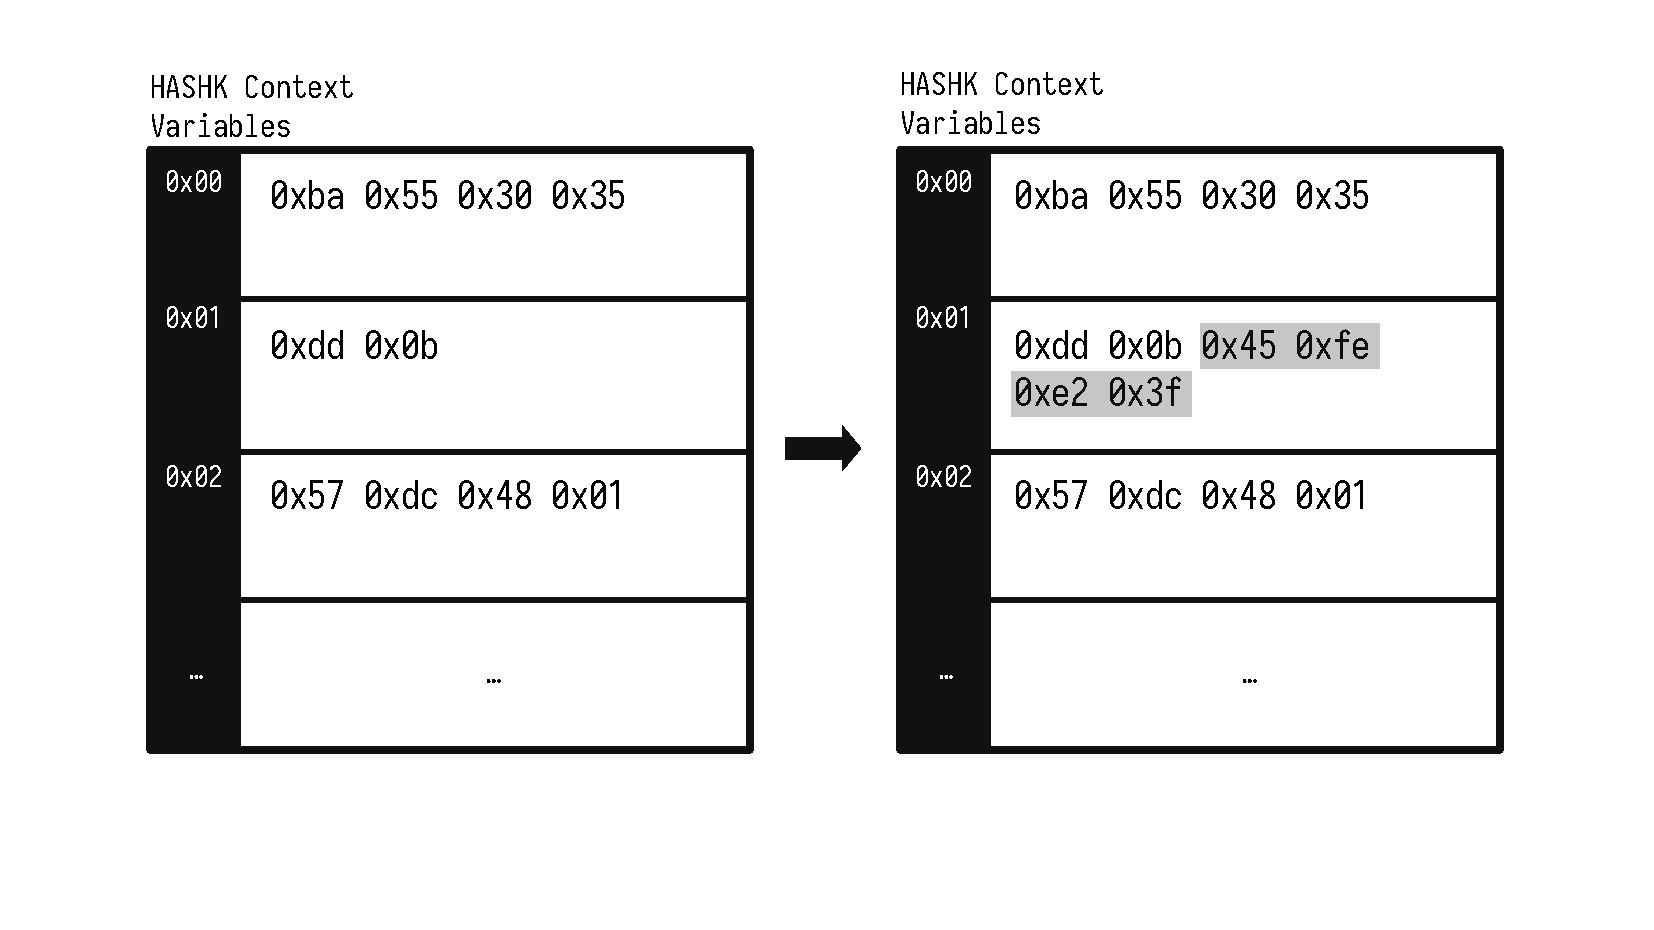
\includegraphics[width=0.6\columnwidth]{\assemblydir/figures/hashk-add-bytes}
    \caption{Schema of the \HASHK instruction.}
    \label{fig:hashk-add-bytes}
\end{figure}

The typical use of the \HASHK instruction in the zkASM language is the following one:

\begin{zkasm}
    op	:HASHK(addr)
\end{zkasm}

The \op placeholder will usually be a register or a register operation like the following one: 

\begin{zkasm}
    A + 1	:HASHK(addr)
\end{zkasm}

We can perform several hashes at the same time, each of them being stored in its corresponding address. Then, we can keep filling each of the addresses' bytes without perturbing the other ones. We can specify the address using the register \E, which is the one used to store addresses $256$-bits, or using a hard coded number. The value $0$ is usually used as an address, which is reserved for storing specific hashes. %TODO: what hashes?

\begin{zkasm}
    A + 1	:HASHK(E)
\end{zkasm}

The former instruction will append the bytes of the current value of \A + 1 into the input of the hash function we want to perform within the bytes attached to the address \E. 

To formalise what the \HASHK instruction does, let $(\op_0, \op_1, \dots, \op_{31})$ be the byte decomposition of the \op variable. We will denote $\mathtt{trunc_{D_0}}(\op)$ by the byte decomposition of \op truncated at the $\mathtt{D_0}$ position. More precisely, 
\[
\mathtt{trunc_{D_0}(\op)} = (\op_0, \op_1, \dots, \op_{\D_0-1}).
\]

Let $\mathtt{hashk}[\texttt{addr}] = (h_0, \dots, h_{\texttt{HASHPOS}})$ be the current array of bytes that we are willing to hash at a certain address \texttt{addr}. The \HASHK instruction will append the $\mathtt{trunc_{D_0}}(\op)$ array into the $\mathtt{hashk}$ one, so that the next state of the (temporal) input of the hash will become 
\[
\mathtt{hashk}[\texttt{addr}] \nextStep = (h_0, \dots, h_{\texttt{HASHPOS}}, \op_0, \op_1, \dots, \op_{\D_0-1})
\]

At the end of this operation, we increase the value of the \texttt{HASHPOS} register in $\mathtt{D_0}$:
\[
\mathtt{HASHPOS} \nextStep = \mathtt{HASHPOS} + \mathtt{D_0}.
\]

Let us propose the following simple example: suppose that we want to hash a single byte concatenated with the first $31$ bytes of a $32$-bytes integer, each of them contained in the registers $\A$ and $\B$ respectively. To that we will use the address \texttt{0x03} stored in the register \E. First of all, we should ensure that our current hash position is $0$, because we are actually starting a new hash.

\begin{zkasm}
    0x03 => E
    0 => HASHPOS
\end{zkasm}

At this moment
\[
\texttt{hashk}[\texttt{0x03}] = \emptyset.
\]

Later on, we will start adding the single byte of \A into the hash input. Observe that we should assign the length $1$ into the register \D because we need to specify the length value in bytes when using the \HASHK instruction. 

\begin{zkasm}
    1 => D
    A				:HASHK(E)
\end{zkasm}

Now, we update the array
\[
\texttt{hashk}[\texttt{0x03}] = (a)
\]
where $a$ denotes the current value of the register \A. Moreover, \texttt{HASHPOS} increased in $1$:
\[
\texttt{HASHPOS} \nextStep = \texttt{HASHPOS} + 1.
\]

Now, we do the same with the register \B

\begin{zkasm}
    31 => D
    B				:HASHK(E)
\end{zkasm}

Finally, the corresponding hash array is the following
\[
\texttt{hashk}[\texttt{0x03}] = (a, b_0, b_1, \dots, b_{30})
\]
where $(b_0, \dots, b_{30}) = \mathtt{trunc}_{31}(\B)$ are the first $31$ bytes of the register \B, which is actually the string we want to hash. Moreover, \texttt{HASHPOS} increased in $31$:
\[
\texttt{HASHPOS} \nextStep = \texttt{HASHPOS} + 31.
\]


\subsubsection{\HASHKONE}

The instruction \HASHKONE performs in the same way that \HASHK but the register $\D_0$ is not relevant here, because the size of the input string is always of $1$ byte. 


\subsubsection{\HASHKLEN}

As commented before, this instruction is actually the one that computes the hash digest and stores it internally, to later on be acquired via the \HASHKDIGEST instruction. This instruction also uses the first $32$ bytes of the \op intermediate value in order to specify the length within all the bytes stored in the specified address that will be hashed. Therefore, the total amount of bytes we can hash is $2^{32}$. 

\begin{figure}[H]
    \centering
    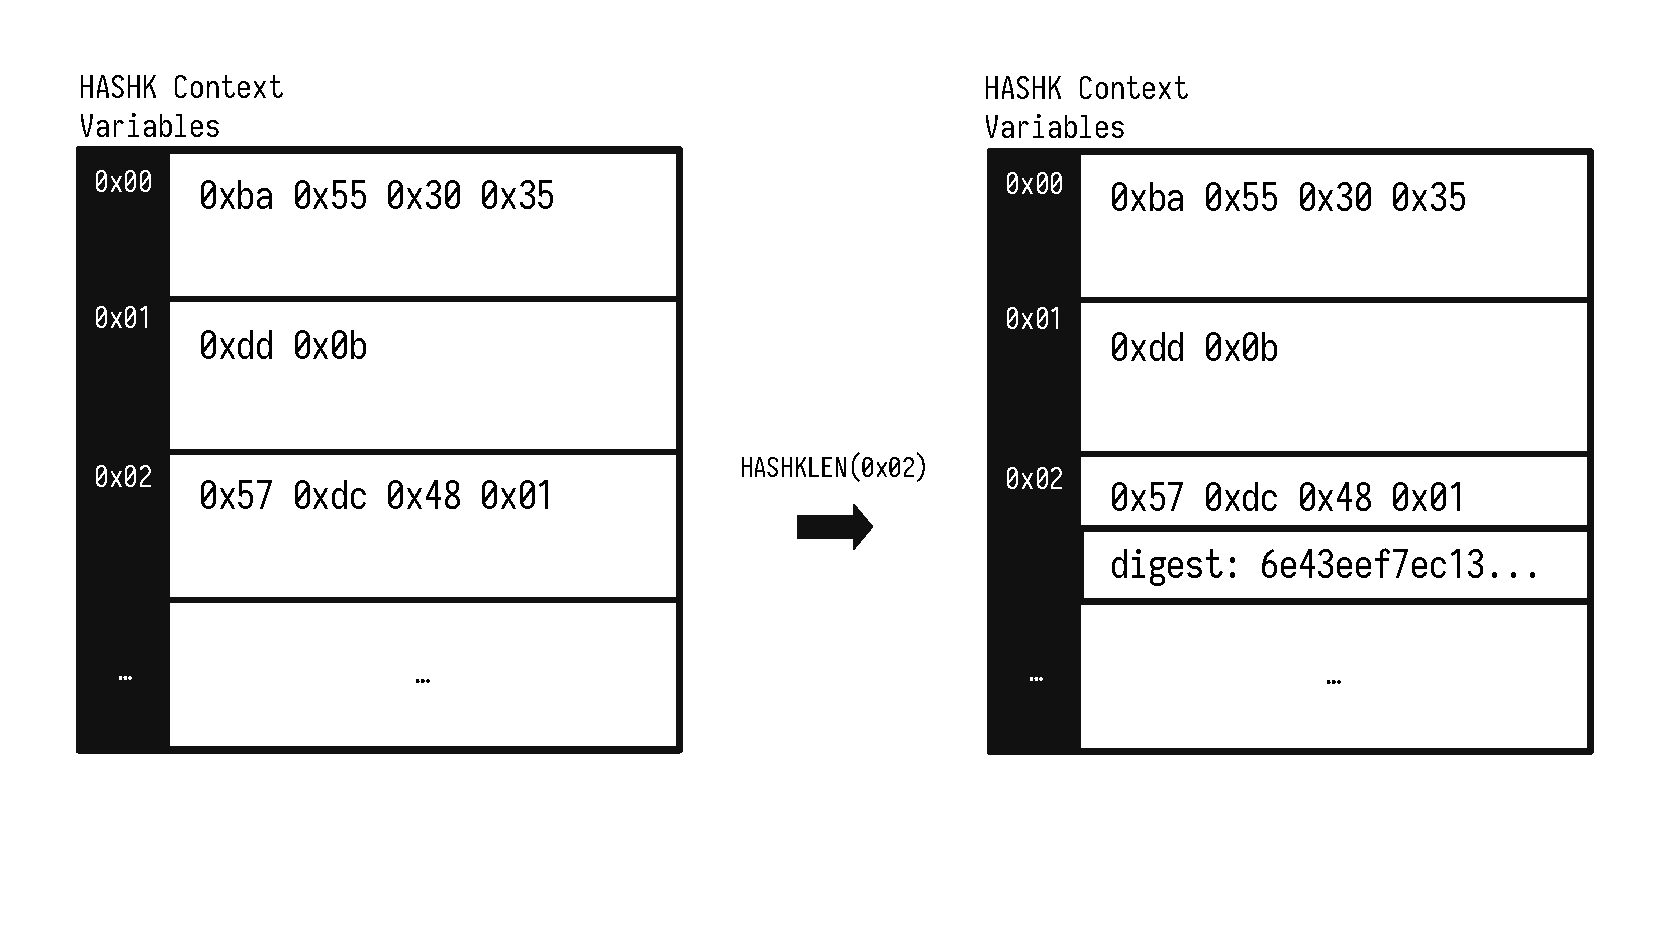
\includegraphics[width=0.6\columnwidth]{\assemblydir/figures/hashklen}
    \caption{Schema of the \HASHKLEN instruction.}
    \label{fig:hashklen}
\end{figure}


Following the previous example, the line of zkASM that we need to execute in this step is the following one:

\begin{zkasm}
    HASHPOS	:HASHKLEN(E)
\end{zkasm}

Recall that \texttt{HASHPOS} value at the current state is $32$ because we want to hash a total amount of $32$ bytes. 


More specifically, if $(h_1, \dots, h_k)$ is the input array attached to a specific address $\texttt{addr}$ (that is, $\mathtt{hashk}[\texttt{addr}] = (h_1, \dots, h_k)$ with the previous notation), the instruction

\begin{zkasm}
    len		:HASHKLEN(addr)
\end{zkasm}

internally stores the digest
\[
d = \texttt{KECCAK-256}(h_1, \dots, h_k).
\]

Observe that we should have that $k = \texttt{len}$. Otherwise, the \HASHKLEN instruction will get an error. % TODO: This checks are checking the integrity of the memory?




\subsubsection{\HASHKDIGEST}

This usual way we are invoking this instruction is the following 

\begin{zkasm}
    $ => REG	:HASHKDIGEST(E)
\end{zkasm}

Meaning that we are storing the digest of the hash attached to the address $\E$ into the register \texttt{REG}. The hash digest is introduced as a free input using the \texttt{\$ =>} operator. In our example, if we want to assign the digest of the hash to the register \D, we would use the following line

\begin{zkasm}
    $ => D		:HASHKDIGEST(E)
\end{zkasm}


%TODO: Counters needs to be incremented.





\newpage
\bibliographystyle{alpha}
\bibliography{../bib/bibliography}


\end{document}

